\documentclass[phd,electronic,oneside,letterpaper,chaptercenter,parttop,lof,lot,prettyheadings,duplexprinter]{byumsphd}

\usepackage[
    bookmarks=true,
    bookmarksnumbered=true,
    breaklinks=false,
    raiselinks=true,
    pdfborder={0 0 0},
    colorlinks=false,
    plainpages=false,
    ]{hyperref}
    
% This makes hyperlinks point to the tops of figures, not their captions
\usepackage[all]{hypcap}

% These packages allow the bibliography to be sorted alphabetically and allow references to more than one paper to be sorted and compressed (i.e. instead of [5,2,4,6] you get [2,4-6])
\usepackage[numbers,sort&compress]{natbib}
%Commented out by Jie
%\usepackage{hypernat}
%Added by Jie
\usepackage{graphicx}
\graphicspath{{../fig/}}
\DeclareGraphicsExtensions{.pdf,.jpeg,.png,.jpg,.eps}
\usepackage{caption}
\usepackage{subcaption}
%\usepackage{makeidx}
%\makeindex


%Added by Lanny
\usepackage{indentfirst}
\usepackage{amsmath}
\usepackage[titletoc]{appendix}
\usepackage{multirow}
\usepackage{array}
\usepackage{algpseudocode}
\usepackage{epstopdf}
\newcommand{\rr}{\raggedright}
\newcommand{\tn}{\tabularnewline}
\newcommand{\shortcite}[1]{\cite{#1}}
\newcommand{\degree}{\ensuremath{^\circ}}



% Because I use these things in more than one place, I created new commands for
% them.  I did not use \providecommand because I absolutely want LaTeX to error
% out if these already exist.
\newcommand{\Title}{Managing Autonomy by Hierarchically Managing Information: Autonomy and Information at the Right Time and the Right Place}
\newcommand{\Author}{Lanny Lin}
\newcommand{\GraduationMonth}{December}
\newcommand{\GraduationYear}{2013}

% Set up the internal PDF information so that it becomes part of the document
% metadata.  The pdfinfo command will display this.
\hypersetup{%
    pdftitle=\Title,%
    pdfauthor=\Author,%
    pdfsubject={PhD Dissertation, BYU CS Department: %
                Degree Granted \GraduationMonth~\GraduationYear, Document Created \today},%
    pdfkeywords={Unmanned Systems, Path Planning, Navigation, Human-Robot Interaction, Adjustable Autonomy, Bayesian Modeling},%
}

% Rewrite the itemize, description, and enumerate environments to have more
% reasonable spacing:
\newcommand{\ItemSep}{\itemsep 0pt}
\let\oldenum=\enumerate
\renewcommand{\enumerate}{\oldenum \ItemSep}
\let\olditem=\itemize
\renewcommand{\itemize}{\olditem \ItemSep}
\let\olddesc=\description
\renewcommand{\description}{\olddesc \ItemSep}

% Important settings for the byumsphd class.
\title{\Title}
\author{\Author}

\committeechair{Michael~A.~Goodrich}
\committeemembera{Bryan~S.~Morse}
\committeememberb{Mark~Colton}
\committeememberc{Kevin~Seppi}
\committeememberd{David~Embley}

\monthgraduated{\GraduationMonth}
\yeargraduated{\GraduationYear}
\yearcopyrighted{\GraduationYear}

\input{0Abstract.tex}

\documentkeywords{%
    Unmanned Systems, Path Planning, Navigation, Human-Robot Interaction, Adjustable Autonomy, Bayesian Modeling
}

\input{1Acknowledgments.tex}

\department{Computer~Science}
\graduatecoordinator{Quinn~Snell}
\collegedean{Thomas~W.~Sederberg}
\collegedeantitle{Associate~Dean}

% Customize the name of the Table of Contents section.
\renewcommand\contentsname{Table of Contents}

% Remove all widows and orphans.  This is not normally recommended, but in a
% paper dissertation there is no reasonable way around it; you can't exactly
% rewrite already-published content to fix the problem.
\clubpenalty 10000
\widowpenalty 10000

% Allow pages to have extra blank space at the bottom in order to accommodate
% removal of widows and orphans.
\raggedbottom

% Produce nicely formatted paragraphs. There is nothing additional to do.  In
% case you get some problems, surround your text with
% \begin{sloppy} ... \end{sloppy}. If that does not work, try
% \microtypesetup{protrusion=false} ... \microtypesetup{protrusion=true}
\usepackage{microtype}

\begin{document}

% Produce the preamble
\microtypesetup{protrusion=false}
\maketitle
\microtypesetup{protrusion=true}

\chapter{Background, Motivation, and Overview}
\label{chap:intro}

%=====================================================================================================
\section{Introduction}
\label{intro}
%About 5 pages answering questions 1 and 2 above, along with describing the broad research area. This section provides the reader with enough information to understand and appreciate the thesis statement. This includes giving the motivation for the research, defining terms and formulating the problem. Often, subsections labeled ``Background'' and ''Motivation'' will be included in this section. This section typically provides answers to the questions ``What problem do you want to solve'' and ''Who cares about this problem and why?'' The Background subsection could contain the discussion about the broader research area.

%===================================================
\subsection{Problem Motivation}
\label{motivation}

Because of rapid advancement in technology, more and more Artificial Intelligence (AI) and robotics systems are appearing in various aspects of people's lives. For example, there are systems that assist humans to schedule limousine services~\cite{Chun2010Limousine}, to evaluate and control the damage of an oil spill\footnote{http://spectrum.ieee.org/robotics/industrial-robots/the-gulf-spills-lessons-for-robotics}, to support search and rescue missions~\cite{Casper2003Human,Lin2010Supporting}, and to provide treatment to children with autism~\cite{Robins2009From}. Such abundant and rapidly growing applications increase the set of possible interactions between human users and autonomous systems. The humans in such interactions are not likely the designers of the autonomous systems, but these humans must still manage the autonomy.

Although AI and robotics systems have grown to be able to handle increasingly complex tasks in uncertain environments, human assistance and supervision are often needed~\cite{Bainbridge1983Ironies}. Even for fully autonomous systems, human input can potentially improve the system's performance and safety. Human experts can use domain-specific knowledge to assist an AI/robotics system when it deals with changing environments, uncertainty, and case-specific scenarios. Therefore, it is necessary to design tools and interfaces that enable human users working with an AI/robotics system to manage the autonomous behaviors of the system efficiently and effectively; such tools can improve task performance and the experience of a human partner in human-autonomy interaction. 

However, human users often do not understand how the internal mechanisms of an autonomous system work especially when the system is complicated or when complex algorithms are involved. Instead, humans must rely on their own mental models of the system during operation~\cite{Moray1999Mental}. Supporting human interaction requires a design approach that lets users understand how autonomous behaviors can be influenced without getting deeply into how autonomy really works. This requirement makes designing for autonomy management especially challenging.

%===================================================
\subsection{General Solution Approach}

We propose that autonomy management tools should let users hierarchically manage information provided to an AI/robotics system. Good information management tools should allow users to influence the autonomous behaviors of the system at multiple scales without the need for tedious direct/manual control. This dissertation presents autonomous algorithms/components and autonomy management tools/interfaces designed at different scales and show that this approach improves the performance of the human-autonomy team and the experience of the human-autonomy interaction.

The term ``information'' here covers a wide range of things including \textit{knowledge of the environment} (including other humans, equipment, and changes in the physical surroundings), \textit{knowledge of the task} at hand (including processes, procedures, rules, past experiences, etc.), and \textit{interactions among various entities} (task, environment, human, and the system). In theory, an AI/robotics system can obtain, process, and analyze information in order to complete the desired tasks. In practice, however, the system often has limited sensing and reasoning capabilities, and there is useful information the system is either not capable of obtaining or not able to understand/process. Such information can even be produced by the system itself. Often, the human users of such systems have much better ``information sensing'' capabilities. These capabilities allow humans to obtain information from their own resources such as past experiences, domain-specific training, external communications (with team members, external systems, etc.), or even the AI/robotics system itself. The human user is also capable of ``digesting'' various information and then feeding the ``filtered'' information to the system in forms the system can understand. In a sense, the human user acts as an ``intelligent sensor'' for the system. At the same time, by deciding what information to provide to the system, the human user has a way of influencing the system's autonomous behaviors without the need for tedious manual control.

%\begin{figure}
%\centering
%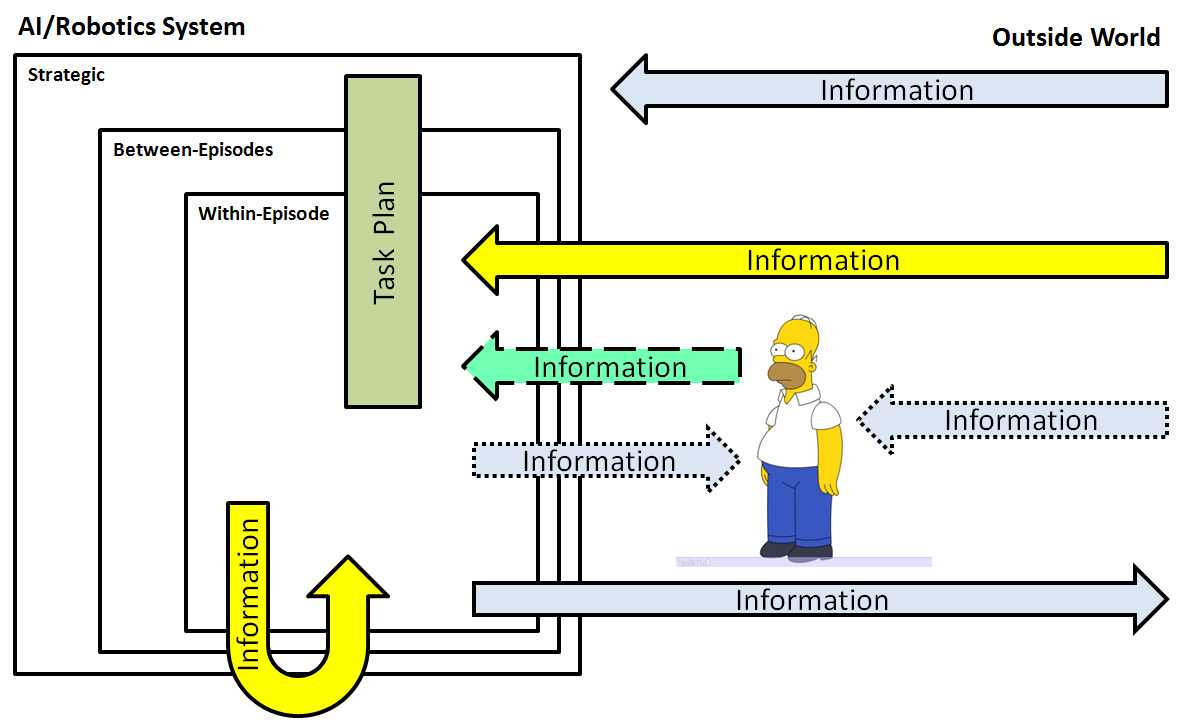
\includegraphics[width=4.5in]{System.png}
%\caption{Diagram showing relationship between the human user and the AI/robotics System with respect to information management.}
%\label{system}
%\end{figure}

%Figure~\ref{system} shows a diagram of the relationship between the human user and the AI/robotics system. The system must be capable of receiving the outside information at different scales (solid yellow arrow at the top). The system has some degree of sensor-processing, so it naturally uses internal information to make decisions (solid yellow arrow at the bottom). The human can sense and process information the system is not capable of handling. Such information can be directly from the outside world (dotted blue arrow on the right) or perceived through the system's sensors (dotted blue arrow on the left). The human processes the information and feeds filtered information to the system, in forms the system can understand (dashed green arrow), in order to influence the system's autonomous behaviors.

\begin{figure}
\centering
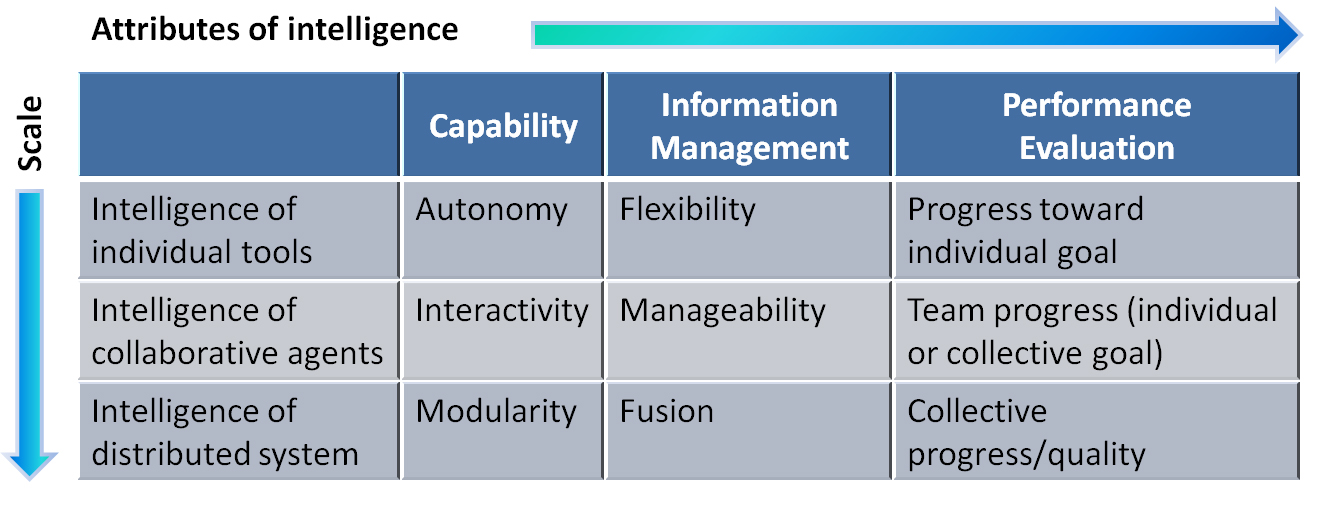
\includegraphics[width=6in]{IntegrationChallenges.JPG}
\caption{Autonomy integration challenges defined along two dimensions. Horizontal dimension: attributes of intelligence. Vertical dimension: scale.}
\label{challenges}
\end{figure}

In an overall integrated intelligent system, autonomy typically exists as component tools with the goal to offload portions of responsibility to autonomous algorithms. Figure~\ref{challenges} lists some key elements of the autonomy integration challenges we identified in~\cite{Lin2010Supporting} along two dimensions: \textit{attributes of an intelligent system} (capability, information management, performance evaluation) and \textit{scale} (individual versus group, expanded to include a new row for intelligence of collaborative agents). This table provides guidelines on what attributes should be designed into an autonomous component when it is part of a human-autonomy collaboration team and a much larger distributed intelligent system. 

As an individual tool, the autonomous component needs to be able to perform certain tasks (\textbf{autonomy}). It should be able to work with different scenarios and can be interrupted, temporarily aborted, and possibly resumed later depending on information available to the operator (\textbf{flexibility}). 

If a human agent is in a collaborative team with the autonomous agent, the autonomous component must provide ways of interaction (\textbf{interactivity}) so the human can manage how the autonomous component works based on information only the human can interpret (\textbf{manageability}). It is different from flexibility because the human agent can actually influence the behaviors of the autonomous component through information management. 

Then in order to integrate the autonomous component into the overall distributed system, the autonomous component has to be modular so it is easy for human operators to share responsibilities or (partially) take on responsibilities of different roles (\textbf{modularity}). Information from various sources (including information output from autonomous components) needs to be combined and presented intelligently in an efficient way to relevant users (\textbf{fusion}). Autonomous components presented in this dissertation all contain these important attributes. Specifically, we design our autonomous components with the capability to interact with information representations so the human agent can manage autonomy by hierarchically managing information. 

Good autonomy management tools will only let users manage information that allow them to develop a clear causal relationship between information management actions and the changes of the system's autonomous behaviors. Examples of such information include what data set to use to train the system and which tasks deserve more attention. Such causal relationships make developing correct mental models of the system easier leading to improved task performance~\cite{Moray1990Lattice}. 

Information can be managed at different temporal scales. 
%We use the term ``resolution'' to describe the levels of details involved. Working at a high resolution is like working with individual pixels in an image to achieve fine precision, whereas working at a low resolution is more like working on object attributes such as shapes or shadings that are viewed better when one takes a step back from the image and ignores the fine details. Similarly, managing autonomy at a high resolution involves managing the actions of the AI/robotics system in fine details (e.g., managing waypoints a UAV should follow), and at a low resolution autonomy management might deal with strategic planning following generate trend (e.g., predicting and identifying high priority areas in a WiSAR operation).
We propose a general hierarchical framework that focuses on the following three scales: \textbf{strategic}, \textbf{between-episodes}, and \textbf{within-episode}\footnote{The term ``episode'' we use is similar to the one Russell and Norvig define in Chapter 2 of~\cite{Russell2009Artificial} when they discussed episodic vs. sequential task environments. Our definition is more relaxed to include cases where actions taken in previous episodes might impact the current episode with respect to task objectives, but each episode is still by itself a separate and self-contained unit.}. 

When an AI/robotics system is given a task, the system can generate an initial plan based on its model(s) of how this kind of task is generally performed. This plan looks at the task as a whole from a high level, prioritizes areas of focus, and determines how resources should be allocated accordingly. Such a plan is normally used throughout the entire process. Therefore, this step is planning at the \textbf{strategic} scale (e.g., deciding where are likely places to find a missing person in a WiSAR scenario and what kind of search team to send to those areas). Since the same task can be performed in different case scenarios (such as different environments, constraints, or phases of the operation) or repeated (such as multiple sessions), case-specific attributes and requirements need to be evaluated, and the initial plan needs to be tailored to the specific case or episode. This step is planning at the \textbf{between-episodes} scale. (e.g., each time a manned/unmanned plane finishes a round of searching). During execution of the task, the plan is carried out, but as new information becomes available or when the environment changes due to uncertainty, the plan can be modified in real time to achieve better task performance. This step is planning at the \textbf{within-episode} scale (e.g., while a manned/unmanned plane is still in the air searching). If the user of the system can manage information provided to the system by selecting what information to provide at what scale, he/she can change the system plan at different scales and indirectly influence the autonomous behaviors of the system.

To evaluate the usefulness of the proposed autonomy management approach, we apply it to the application domain of using an Unmanned Aerial Vehicle (UAV) to support Wilderness Search and Rescue (WiSAR).

%===================================================
\subsection{Application Domain}

A small camera-equipped UAV can quickly and cheaply provide aerial imagery of a wilderness search area, especially hard-to-reach areas~\cite{Goodrich2008Supporting}. The MAGICC lab, the HCMI lab, and the Computer Vision Lab at BYU have been researching UAV technologies for several years and made great progress in UAV path-planning control, user interface design, and computer vision~\cite{Lin2010Supporting}. Figure~\ref{SystemComponents} shows the various components developed by the research group. This dissertation focuses on the three highlighted components that are related to the UAV path planning problem.

\begin{figure}
\centering
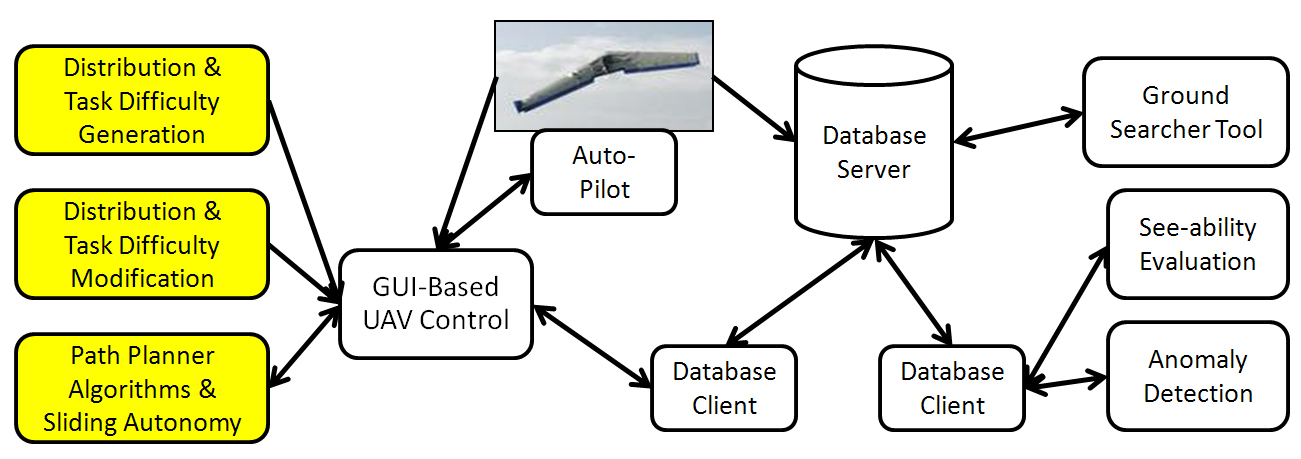
\includegraphics[width=6in]{UAVWiSARComponents.JPG}
\caption{Various components of the overall intelligent system (a distributed system) of using a UAV to support Wilderness Search and Rescue. The three highlighted components are related to UAV path planning.}
\label{SystemComponents}
\end{figure}

Past UAV field trials indicate that real WiSAR searchers like not having to worry about keeping the UAV in the air or setting waypoints manually. Autonomy that offloads or complements some search work is useful, but searchers also need to be able to manage where to send the UAV as new evidence is gathered or hard-to-reach areas are identified. Ideally, searchers need not understand the statistical models or complex algorithms used by the UAV. Rather, searchers should manage autonomy by managing information provided to the UAV system at different scales. We focus on two important representations of information: a \textit{probability distribution map} and a \textit{task-difficulty map} as shown in Figure~\ref{Scales}.

\begin{figure}
\centering
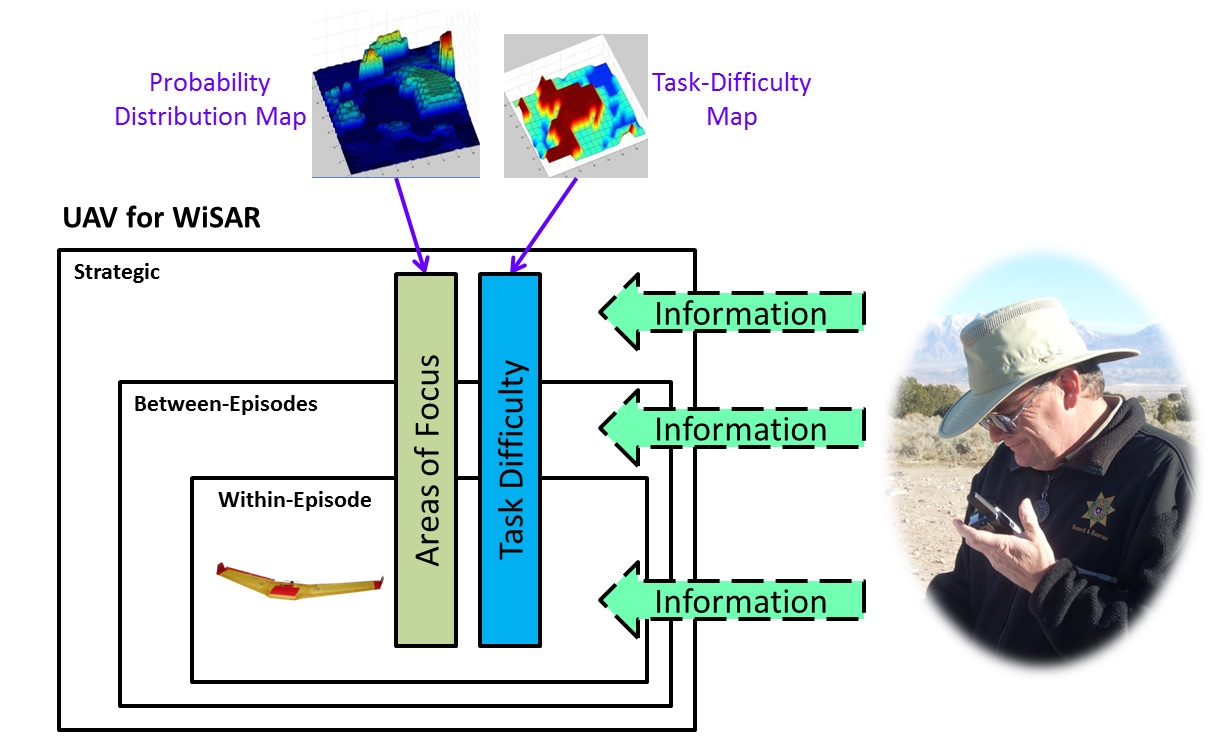
\includegraphics[width=6in]{scales.JPG}
\caption{WiSAR searchers can manage autonomy by managing a \textit{probability distribution map} and a \textit{task-difficulty map} at different scales of the system.}
\label{Scales}
\end{figure}

Following the guidelines in Figure~\ref{challenges}, we developed autonomous components/algorithms and management tools/interfaces that meet the challenges of an integrated system and also support collaboration between a human agent and an autonomous agent at different scales. At  the \textbf{strategic} scale, we developed the \textbf{DistCreate} and \textbf{DiffCreate} components. \textbf{DistCreate} (Chapter~\ref{chap:CMOT2010}) uses a Bayesian model to predict the probability distribution of the missing person's likely location, using terrain features of the search area and past human behavior data in the form of GPS track logs. Domain users can affect the model-generated probability distribution by changing prior beliefs parameters and by determining what human behavior data (data for selected regions, season, or missing person characteristics) to feed to the model. \textbf{DiffCreate} (Chapter~\ref{chap:SMCB2014}) is a simple tool that automatically generates a task-difficulty map, a representation marking areas with low probability of detection, based on vegetation coverage Landsat data from USGS satellite imagery servers\footnote{http://www.usgs.gov/pubprod/}. 

At the \textbf{between-episodes} scale, we developed two management tools: \textbf{DistEdit} (Chapter~\ref{chap:MapEdit}), a tool that lets the user modify the probability distribution to specify areas of focus with simple gestures, and \textbf{DiffEdit} (Chapter~\ref{chap:MapEdit}), a tool that lets the user use scribbles to modify the task-difficulty map. 

At the \textbf{within-episode} scale, we developed a bunch of path planning algorithms that support partial detection and real-time feedback. We also present a \textbf{SlidingAutonomy} interface (Chapter~\ref{chap:JHRI2014}) that lets a human agent manage UAV autonomy along two dimensions: a temporal dimension deciding how much time is granted to a UAV for each path segment, and a spatial dimension determining what  constraints (path segment ending points) to impose to the path planning task.


%=====================================================================================================
\section{Related Work}
\label{related}
%About 2 pages answering question 3 above. This section contains a survey of the literature directly related to the problem you are trying to solve (i.e., thesis statement) and should demonstrate to your readers that you understand the context of your work. This is a place for you to position your contribution to your specific research area relative to other work that has been done, and to state how your work builds on the previous work. In most cases there will be only a small overlap between the papers discussed in this section and the papers related to the broader research area. This section answers the question ``What have others done to solve the problem and why is this inadequate?''

In their in-depth survey paper~\cite{Goodrich2007HRISurvey}, Goodrich and Schultz define the HRI problem as ``understanding and shaping the interactions between one or more humans and one or more robots.'' They also specified robot-assisted search and rescue as a key area for HRI research. In this section we first present related work in the general research area, then discuss related research more specific to the domains of using UAVs to support Wilderness Search and Rescue.

%===================================================
\subsection{General Research Area}

When humans and robots work together as a team, balancing responsibilities between human and autonomy becomes a difficult challenge. Drucker defines automation as a ``concept of the organization of work~\cite{Drucker2006Practice}.'' In their 1978 seminal paper~\cite{Sheridan1978Human}, Sheridan and Verplank propose the idea of a \textit{level of autonomy} spectrum. At one end of the spectrum is full teleoperation and at the other is full autonomy. In the middle of this spectrum, the robot could suggest actions to humans or make decisions before informing humans. Parasuraman et al.\ \cite{Parasuraman2000Model} extended this one-dimensional spectrum to four different broad functions: information acquisition, analysis, decision selection, and action implementation. 

In~\cite{Sheridan1992Telerobotics} Sheridan proposes \textit{supervisory control}, in which a human divides the task into a sequence of subtasks that the robot is capable of performing, and the human then provides guidance when the autonomous system cannot solve a problem on its own. In contrast to the top-down philosophy of supervisory control, a \textit{mixed-initiative} approach advocates the idea of dynamically shifting tasks when necessary~\cite{Hearst1999Mixed}. \textit{Collaborative control}, which can be thought of as an instance of mixed-initiative interaction, is a robot-centric model; instead of the human always being in-charge, the robot is treated as a peer and can make requests to humans through dialogs~\cite{Fong1999Collaborative}. \textit{Adjustable autonomy}~\cite{Dorais2001Designing} (also referred to as \textit{sliding autonomy}~\cite{Dias2008SlidingAutonomy} or \textit{adaptive automation}~\cite{Rouse1988Adaptive}) is another type of mixed-initiative interaction, one that enables the human-autonomy team to dynamically and adaptively allocate functions and tasks among team members. Bradshaw et al.\ \cite{Bradshaw2004Dimensions} propose two dimensions of Adjustable Autonomy (descriptive  and prescriptive) to address the two senses of autonomy (self-sufficiency and self-directedness) and discuss how permissions, obligations, possibilities, and capabilities can be adjusted. Bradshaw et al.\ \cite{Bradshaw2013Seven} also summarized some widespread misconceptions on autonomy and listed seven deadly myths of ``autonomous systems.''

Scholtz defines in~\cite{Steinfeld2006Common} four roles for a human in human-robot interaction: supervisor, operator, mechanic, peer, and bystander. Goodrich and Schultz suggest two more roles: mentor and information consumer~\cite{Goodrich2007HRISurvey}. Humphrey and Adams add another role, abstract supervisor~\cite{Humphrey2009Information}. With our information management approach, users can act as ``intelligent sensors'' and manage what information to feed the system at different scales. Therefore, the human is taking on a smart ``information sensor'' role in HRI. 

The idea of using humans as sensors is not new. For example, Kaber et al.\ advocate using humans as active information processors in complex systems to support situation awareness and effective performance~\cite{Kaber2001Design}. Bourgault et al.\ include humans as augmented sensor nodes in a wilderness search task~\cite{Bourgault2008Human}. Other researchers have experimented with management at different resolution. Dias et al.\ \cite{Dias2008SlidingAutonomy} propose enabling interactions at different levels of granularity. However, using information as a control mechanism to manage autonomy at the three distinctive scales we identified is different from previously published approaches.

One component of our proposed solution, the \textbf{SlidingAutonomy} interface, falls under the category of \textit{Adjustable Autonomy}. Dorais et al.\ \cite{Dorais1998AdjustableAutonomy} discuss a framework for human-centered autonomous systems for a manned Mars mission. The system enables users to interact with these systems at an appropriate level of control but minimize the necessity for such interaction. Bradshaw et al.\ discuss principles and pitfalls of adjustable autonomy and human-centered teamwork, and then present study results on so-called ``work practice modeling'' and human-agent collaboration in space applications~\cite{Bradshaw2003AdjustableAutonomy}. In~\cite{Kaber2005Adaptive} Kaber et al.\ describe an experiment simulating an air traffic control task where manual control was compared to Adaptive Automation (AA). Results suggest that humans perform better with AA applied to sensory and psychomotor information-processing functions than with AA applied to cognitive functions; these results also suggest that AA is superior to completely manual control. Brookshire et al.\ present preliminary results for applying sliding autonomy to a team of robots performing coordinated assembling work to help the system recover from unexpected errors and to thereby increase system efficiency~\cite{Brookshire2004Preliminary}. Dias et al.\ identified six key capabilities that are essential for overcoming challenges in enabling sliding autonomy in peer-to-peer human-robot teams~\cite{Dias2008SlidingAutonomy}.

The human is an integral part of the human-autonomy team. When working with autonomy, the human often takes on the supervisor role. Bainbridge points out that automation requires the human operator to take additional management responsibilities~\cite{Bainbridge1983Ironies}, and Sartar identified in~\cite{Sarter1998Making} two automation management policies: \textit{management by consent} and \textit{management by exception}, defining whether the human always retain authority or can the system take initiative. 

For complex automation, the human tends to rely on his/her \textit{mental models} (defined by Norman in~\cite{Norman1983Some}) to manage the system. Moray~\cite{Moray1999Mental} provides a good summary of how mental models are used and proposes that mental models ``allow operators to think about causal structures and functions in systems which they must control....'' Goodrich and Boer present a case study of Adaptive Cruise Control design and explain how an automobile driver can switch among multiple mental models and use different management strategies~\cite{Goodrich2002Multiple, Goodrich2003Model}. 

Lee and See propose that because people respond to technology socially, trust guides reliance when unanticipated situations make it impractical or impossible to understand automation~\cite{Lee2004Trust}. Hoffman et al.\ \cite{Hoffman2013Trust} suggest ``active exploration for trusting''(AET) and hope this approach can promote both trust ``calibration'' and appropriate reliance. 

Moray also points out that the operator's internal model of the environmental and task dynamics can affect how the operator samples information from the environment, and display interfaces should be designed to attract the right amount of attention~\cite{Moray1990Designing}. In~\cite{Vicente1997Should} Vicente suggests to follow the ecological approach~\cite{Rasmussen1994Cognitive} and design interfaces compatible with the actual constraints of the environment so the operator's understanding corresponds to the actual behavior of the system. Given these principles of interaction, our information management approach and proposed tools are compatible with these principles because they allow a user to infer causal relationship between user actions and autonomous behavior changes. The user interface designs enable the user to develop mental models of the system that match how the system truly works and thereby improve the human-autonomy interaction experience.

Given the user interface and framework for interaction mentioned above, it is necessary to evaluate the usefulness of the resulting system. Properly evaluating human-robot interaction has always been a challenging problem due to the diversity of team setups, environmental contexts, and tasks involved. Many metrics have been proposed in the literature. Crandall and Goodrich proposed a metric called \textit{neglect time} to measure interaction efficiency~\cite{Crandall2002Principles}. Together with neglect time, Olsen and Goodrich later added \textit{task effectiveness}, \textit{robot attention demand}, \textit{fan out}, and \textit{interaction effort} to the list of metrics~\cite{Olsen2003Metrics}. Steinfeld and et al.\ suggest some common metrics for standardizing task-oriented human-robot interaction~\cite{Steinfeld2006Common}. In~\cite{Olsen2007Evaluating}, Olsen presents a set of criteria for evaluating new UI systems. Crandall and Cummings propose in~\cite{Crandall2007Ddentifying} a set of metric classes that can predict how many robots should be in the team and the system effectiveness for single-operator controlling multiple robots. We follow guidelines provided in these papers to validate our proposed solution.

%===================================================
\subsection{Supporting Wilderness Search and Rescue with a UAV}

The goal of our research is to support fielded missions in the spirit of Murphy's work~\cite{Casper2003Human}. UAV technology has emerged as a promising tool in supporting WiSAR~\cite{Murphy2008Cooperative,Bourgault2003Coordinated}. In~\cite{Bourgault2006Optimal, Bourgault2004Coordinated} Bourgault et al.\ describe how to use a Bayesian model to create paths for a single UAV or multiple coordinated UAVs to maximize the amount of probability accumulated by the UAV sensors. In~\cite{Bourgault2008Human} they also include scalable collaborative human systems as augmented sensor nodes and created paths for human ground searchers.

The BYU WiSAR research group has developed a variety of technologies to support Wilderness Search and Rescue with small fixed-wing UAVs~\cite{Beard2005Autonomous, Goodrich2008Supporting, Goodrich2009Towards, Lin2010Supporting}. The UAV system has many autonomous capabilities. The UAV's autopilot can stabilize the UAV during flight, support waypoint following and auto launch/land modes, and provide gimbaled camera control. Simple flight patterns and safety features are available when combining the autopilot with UAV control interfaces~\cite{Beard2005Autonomous, Lin2010Supporting}. These basic UAV capabilities have been greatly extended to provide better WiSAR support: A Bayesian model was developed by Lin and Goodrich~\cite{Lin2010Bayesian} that uses terrain features to predict the likely locations of finding a lost person. Then, Generalized Contour Search~\cite{Goodrich2008Supporting} and intelligent path planning algorithms~\cite{Lin2009UAV,Niedfeldt2010integrated} have been used to automatically generate flight paths for the UAV. A real-time temporally local mosaic technique~\cite{Morse2008Application} has been used to ``stitch'' multiple video frames to provide increased opportunity for detection and increased sense of relative spatial relationships for video analyst. Anomaly detection algorithms~\cite{Thornton2011Unusual} are also available that can mark objects with unnatural colors and alert the video analyst. A metric named ``see-ability''~\cite{Morse2010UAV} was also developed to understand search-related video quality and to index geo-tagged video frames. 

Many path planning algorithms in the literature address obstacle avoidance while planning a path to reach a destination using A*~\cite{Quigley2005Towards}, LRTA*~\cite{Howlett2006Learning}, D*~\cite{Stentz1997Optimal}, Voroni diagrams~\cite{Bortoff2000Path,Beard2005Autonomous}, or probability roadmaps and rapidly-exploring random tree (RRTs)~\cite{Pettersson2006Probabilistic}. Hierarchical heuristics approaches were also developed, such as Hierarchical A* (HA*) by Holte et al.\ ~\cite{Holte1996Hierarchical}, hierarchical task-based real-time path planning by Naveed et al.\ ~\cite{Meuleau2007Hierarchical}, and Hierarchical-AO* (HiAO*) by Meuleau and Brafman~\cite{Naveed2010Hierarchical}. The algorithms we present solve a different path planning problem by generating paths that make efficient use of the limited travel time and maximizing the probability of finding the missing person. This is similar to the Vehicle Routing Problem~\cite{Laporte1992Vehicle} and the Orienteering Problem (OP)~\cite{Golden1987Orienteering}, which is a variation of the Traveling Salesman Problem (TSP) (with names such as Prize-Collecting TSP (PCTSP)~\cite{Gutin2002Traveling} or TSP with profits~\cite{Feillet2005Traveling}), and is known to be NP-Hard~\cite{Sokkappa1990Cost}. Vansteenwegen et al.\ \cite{Vansteenwegen2011Orienteering} gives a good survey on the topic of OP, and listed various approaches such as exact methods~\cite{Laporte1990Selective,Fischetti1998Solving,Ramesh1992Optimal}, approximate heuristic approaches~\cite{Mittenthal1992Insert,Chao1996Fast,Ramesh1992Optimal}, a genetic algorithm approach~\cite{Tasgetiren2000Genetic}, and an ant colony optimization approach~\cite{Liang2006Ant}. These algorithms work well with OP problems that have a small number of nodes (21--100 nodes). However, our path planning problem requires up to 1800 nodes with added challenges of repeated visits and partial detection, which are defined later.
 
In order to intelligently plan paths for a UAV in a WiSAR context, it is necessary to understand missing person behaviors and generate a probability distribution of likely places to find the missing person. Many researchers analyzed past WiSAR cases in order to understand missing person behaviors~\cite{Setnicka1980Wilderness,Hill1998Lost,Syrotuck2000Analysis,Heth1998Characteristics,Koester2008Lost}.~\cite{Syrotuck2000Introduction} describes how to use mathematical models to calculate the probability of detection, probability of area and probability of success. The paper also describes an example search mission. Researchers also looked at systematically utilizing GIS (Geographic Information System) information for search and rescue applications~\cite{Ferguson2008GIS,Soylemez2006Utility}.

Due to factors such as lighting conditions, dense vegetation, or human observer cognitive workload, even when sensor footprint covers the location of the missing person, probability of detection can be less than 1. In the 1950's, Koopman discussed the uncertainties in the act of detecting hostile submarines with radars and proposed a concept called the \textit{instantaneous probability of detection by one glimpse}~\cite{Koopman1956Theory}. He presented simple search algorithms and demonstrated how search effort should be distributed given a prior probability distribution of the target and a known law of detection when only a limited total amount of search effort (or time) is available~\cite{Koopman1957Theory}. 

Over the years, search theory has evolved to be able to deal with more complex search problems. Stone~\cite{Stone1975Theory} presents various search plans with partial detection models using Lagrange multipliers and maximization of Lagrangians in finding stationary target in very basic search problems when no false targets are present. Washburn~\cite{Washburn1981Search} discusses how to construct optimal search paths for different search problems. The author also developed detection models based on radar/sonar and expanded the fundamentals of search theory to include moving targets. More recent work includes~\cite{Niedfeldt2010integrated} where Niedfeldt et al.\ present a UAV path planning algorithm that utilizes probability of detection and maximizes the probability of identifying an object using a N-step lookahead method, and~\cite{Ryan2010particle} where Ryan and Hedrick developed a control formulation for a fixed-wing UAV that minimizes the entropy of an estimate distribution over a receding horizon for searching a moving target over a fixed time horizon. Stone et al.\ used posterior probability maps and successfully located the wreckage of Air France Flight 447~\cite{Stone2011Search}. Metrics such as Koopman's instantaneous probability of detection by one glimpse~\cite{Koopman1956Theory}, ``seeability'' proposed by Morse et al.\ \cite{Morse2010UAV}, and terrain and vegetation information obtained from USGS~\cite{Lin2010Bayesian} can be used to build a task-difficulty map representing probability of detection in different search subregions.

In this dissertation, the UAV technology, human search experts, and associated user interfaces is treated as an intelligent system with the integration of many component autonomous algorithms and user interfaces. Integration at this level requires tremendous effort. Salas and Fiore~\shortcite{Salas2004Team} provide great insights on challenges across people and machines, and across time and space in distributed teams. Sycara and Lewis~\shortcite{Sycara2002Integrating} also asked the questions: 1) can a software agent perform the task? and 2) can the agent's assistance contribute toward team performance? Tso et al.\ ~\shortcite{Tso1999Multi} identified that integrating a UAV into the search task creates at least two roles: a pilot that controls the UAV and a sensor operator that analyzes the sensor outputs. Lessons from other search-related domains~\cite{Drury2003Awareness} show that multiple roles are required and these roles can be supported by autonomy algorithms and user interface technologies. These findings motivate and guide our research in developing UAV technology to support WiSAR operations.

%=====================================================================================================
\section{Thesis Statement}
\label{thesis}
%1 to 2 sentences stating what is to be demonstrated in your dissertation. A clear and concise statement of what is to be demonstrated or developed in your dissertation work. A good thesis statement makes a specific claim that your readers care about. Ideally, your introduction will give your readers the background they need to understand your thesis statement and to conclude that it matters.

Designing autonomous components and autonomy management tools that let users manage information provided to an intelligent system at different scales allow users to influence the autonomous behaviors of the system without the need for tedious direct/manual control. This approach improves both the human's experience during the human-autonomy interaction and the performance of the human-autonomy team.

%=====================================================================================================
\section{Project Description}
\label{project}

%About 5 pages answering question 4 above. This section describes your preliminary ideas on how you might solve the problem and the anticipated contribution your research will make to the field of Computer Science. This section should convince your committee that you are qualified to pursue the research and have high potential to eventually be able to objectively and convincingly defend your thesis statement. This section answers the question ``What is your proposed solution to this problem?''

We propose a new autonomy management approach that lets users manage the autonomous behaviors of an AI/robotics system by hierarchically managing information at different scales. In this section, we describe how we apply the approach to using a UAV to support WiSAR operations, and relate chapters of the dissertation to components of the hierarchical approach. At each scale, we briefly discuss what autonomous components and autonomy management tools we developed, what kind of information the user can manage, and direct readers to the related chapter for more details.
 
%===================================================
\subsection{Solution Overview}

%In this section we show how we apply the proposed autonomy management approach to using a UAV to support WiSAR operations. We describe the designs and requirements of autonomy management tools at each scale and resolution and how they enable users to manage the autonomy behaviors of the UAV system by managing information.

\begin{figure}
\centering
\begin{tabular}{cc}
	\begin{minipage}{0.45\textwidth}
	\centering
	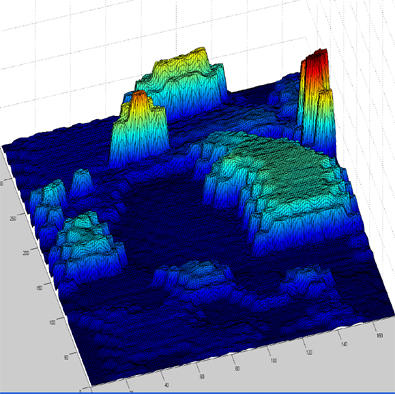
\includegraphics[width=2.8in]{3DMapDist.jpg}
	\caption{An example probability distribution map generated by a Bayesian model.}
	\label{3DMapDist}
	\end{minipage}
&
	\begin{minipage}{0.45\textwidth}
	\centering
	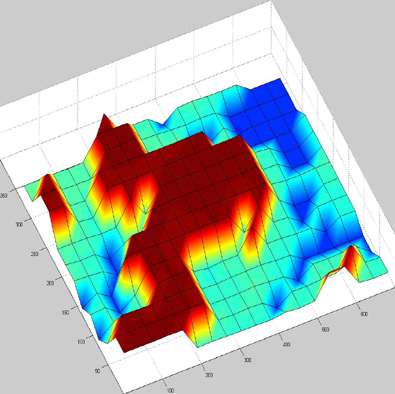
\includegraphics[width=2.8in]{3DMapDiff.jpg}
	\caption{An example task-difficulty map generated using vegetation coverage data with three difficulty levels.}
	\label{3DMapDiff}
	\end{minipage}
\end{tabular}
\end{figure}

When using a UAV to support WiSAR operations, there are two important representations of information: a \textit{probability distribution map} and a \textit{task-difficulty map}. The probability distribution map encodes information about the likely location of the missing person and is illustrated in Figure~\ref{3DMapDist}. In the figure, high values correspond to areas with high probability. The task-difficulty map encodes information about how likely it is for a searcher to detect the missing person if they were in a particular location. Figure~\ref{3DMapDiff} illustrates a task-difficulty map with high values arising from areas with, for example, dense vegetation or low visibility, indicating that likely detection is low in that area. 

From a Bayesian perspective, the probability distribution map encodes prior and posterior beliefs, and the task-difficulty map encodes (one minus) the likelihood of detection. Both maps are needed for effective resource allocation and task prioritization. Throughout the operation, domain experts can process information only available to them or not comprehensible by autonomous components and then incorporate such information into the \textit{probability distribution map} and the \textit{task-difficulty map} at different scales (hierarchies), thus managing autonomy by influencing the behavior of the autonomous components through information management. 

These two maps can be created systematically using statistical models at the strategic scale by using general trends from reliable sources, acting as the general plan for resource allocation used throughout the entire search operation. They can be easily modified by users at the between-episodes scale to incorporate additional case-specific information obtained from the previous episode of searching. They can then be used to facilitate resource allocation and UAV path planning at the within-episode scale while the UAV is in the current episode of searching. 

%\begin{table}
%\centering
%		\begin{tabular}{|l|c|c|}
%			\hline
%				& \multirow{2}{*}{\textbf{Probability Distribution Map}} & \multirow{2}{*}{\textbf{Task-Difficulty Map}}  \\
%				& & \\
%			\hline
%				\multirow{2}{*}{\textbf{Strategic}} & \textbf{TBMod} for map creation &  \\
%				& \textbf{ParamMod} for info management & \\
%			\hline
%				\multirow{2}{*}{\textbf{Between-Episodes}} & \textbf{DistMod} for map update &  \textbf{DiffMod} for map update \\
%				& and info management & and info management \\
%			\hline
%				\multirow{3}{*}{\textbf{Within-Episode}} & Extending algorithms to support & Extending algorithms to support\\
%				& real-time feedback &  partial detection \\ \cline{2-3}
%				& \multicolumn{2}{|c|}{\textbf{SlideMod} for info management} \\
%			\hline
%		\end{tabular}
%	\caption{Components of proposed work}	
%	\label{components}
%\end{table}

\begin{figure}
\centering
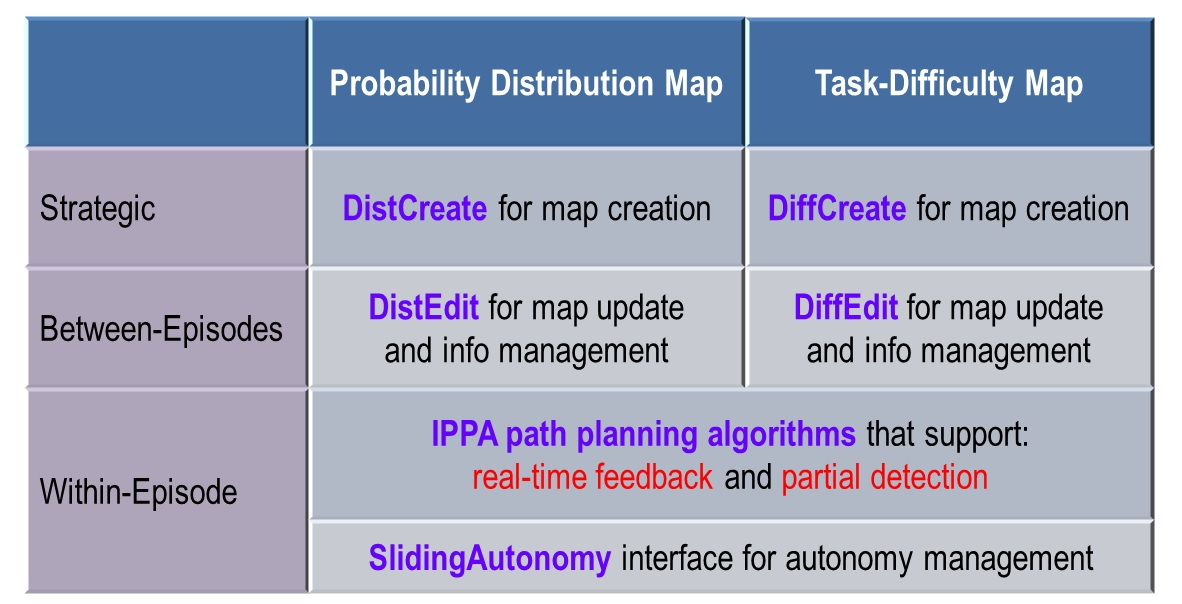
\includegraphics[width=6in]{ProjectComponents.JPG}
\caption{Autonomous components and autonomy management tools of the dissertation work at each scale/hierarchy.}
\label{ProjectComponents}
\end{figure}

Figure~\ref{ProjectComponents} lists the various components of the dissertation work as they relate to these two map representations. At the strategic scale, the \textbf{DistCreate} component uses a Bayesian model to systematically generate the probability distribution map, and the \textbf{DiffCreate} component uses Landsat data to automatically generate the task-difficulty map. At the between-episodes scale, the \textbf{DistEdit} tool and the \textbf{DiffEdit} tool enable the user to modify the probability distribution map and the task-difficulty map respectively. At the within-episode scale, we developed multiple intelligent path planning algorithms (\textbf{IPPA}) to support real-time feedback and partial detection. We also built an information management tool, \textbf{SlidingAutonomy}, that lets the user prioritize search regions and manage the amount of autonomy desired.

All the autonomous components and autonomy management tools were designed following autonomy integration guidelines we defined in~\cite{Lin2010Supporting} (Chapter~\ref{chap:AAAI2010} of the dissertation). Figure~\ref{challenges} lists the challenges along two dimensions: \textit{attributes of an intelligent system} (capability, information management, performance evaluation) and \textit{scale} (individual, collaborative, distributed). Specifically, all the autonomous components we designed allow interactivity through the \textit{probability distribution map} and the \textit{task-difficulty map}, which enables the human agent to manage the behavior of autonomy. Additionally, the \textbf{SlidingAutonomy} management tool lets the human agent interact and manage path planning autonomy through (temporal) time allocation and (spatial) constraints (Chapter~\ref{chap:JHRI2014} of the dissertation). Chapter~\ref{chap:AAAI2010} also describe in detail how the UAV path planning problem we are solving fits in the overall intelligent system of using UAVs to support Wilderness Search and Rescue. 

%===================================================
\subsection{At the Strategic Scale}

At the strategic scale, a probability distribution map and a task-difficulty map can be created systematically.

We established in~\cite{Lin2010Bayesian} (Chapter~\ref{chap:AAAI2010} of the dissertation) a Bayesian model (\textbf{DistCreate}) that can generate the probability distribution map systematically using three types of terrain features (topography, vegetation, and elevation) and past human behavior data. Searchers first specify transitional probabilities (Beta distributions) between two terrain features as inputs. Then the model produces the prior/posterior~\cite{Russell2009Artificial} predictive probability distribution(s), which can be used to allocate resources and plan UAV paths. Figure~\ref{3DMapDist} shows an example posterior predictive probability distribution map generated by \textbf{DistCreate}. The user can influence the model-generated probability distribution by managing two types of information: \textit{model parameters} and \textit{dataset}. 

We represent the probability distribution map in discretized form using a hexagonal tessellation of the search region. We use Monte Carlo methods to encode changes in the map, so \textit{model parameters} include the users prior belief of the transition probabilities (probability of a missing person moving from one hexagonal cell to a neighbor). This approach is based on the assumption that transition probabilities are easily interpreted by search experts, but algorithm parameters are not. 

Although the term ``dataset'' can broadly include many sources of data, here we refer to GPS track logs of past human behavior. The user can choose whether or not to use past human behavior data. If the user chooses not to use past human behavior dataset, the \textbf{DistCreate} model will output the prior predictive distribution (prediction based only on the model parameters); otherwise, the model will output the posterior predictive distribution (prediction also based on past observations). The user can also choose what subset of the dataset to use, filtering past human behavior data by categories such as season of the year, region, or missing person profile. The user's choice will indirectly affect the probability distribution map generated by the Bayesian model.

The \textbf{DistCreate} component at this scale can download terrain vegetation coverage Landsat data directly from the USGS satellite image servers in real time when provided with GPS coordinates. Then it generates a task-difficulty map based on the type of vegetation in the specified region using a lookup table. For example, grassland is categorized as sparse vegetation and marked as easy detection area; shrub is categorized as medium vegetation and marked as medium detection area; evergreen forest is categorized as dense vegetation and marked as difficult detection area. Therefore, this component only utilizes vegetation density information when considering the difficulty level in sensor detection. Figure~\ref{3DMapDiff} shows an example task-difficulty map generated by \textbf{DiffCreate}. It is a very simple model, and we include it for completeness. Since it is modular, it can be easily extended or replaced by a more advanced detection model where factors such as ``seeability''~\cite{Morse2010UAV} (lighting condition, viewing angle, etc.) and video observer cognitive workload can be incorporated.

%===================================================
\subsection{At the Between-Episodes Scale}

At the between-episodes scale, a searcher might have additional case-specific information (e.g, past experience, knowledge of the search area or weather conditions, or the profile of the missing person) and would like to modify the general plan produced at the strategic scale. Moreover, as search progresses, the search plan should change due to newly found evidence (or the lack of it) from either the ground searchers or previous UAV flights. We developed two autonomy management tools at this scale that allow the user to manage two types of information: \textit{areas of focus} and \textit{task difficulty}. Chapter~\ref{chap:MapEdit} explains how these two tools work in detail.

\begin{figure}
\centering
\begin{tabular}{cc}
	\begin{minipage}{0.45\textwidth}
	\centering
	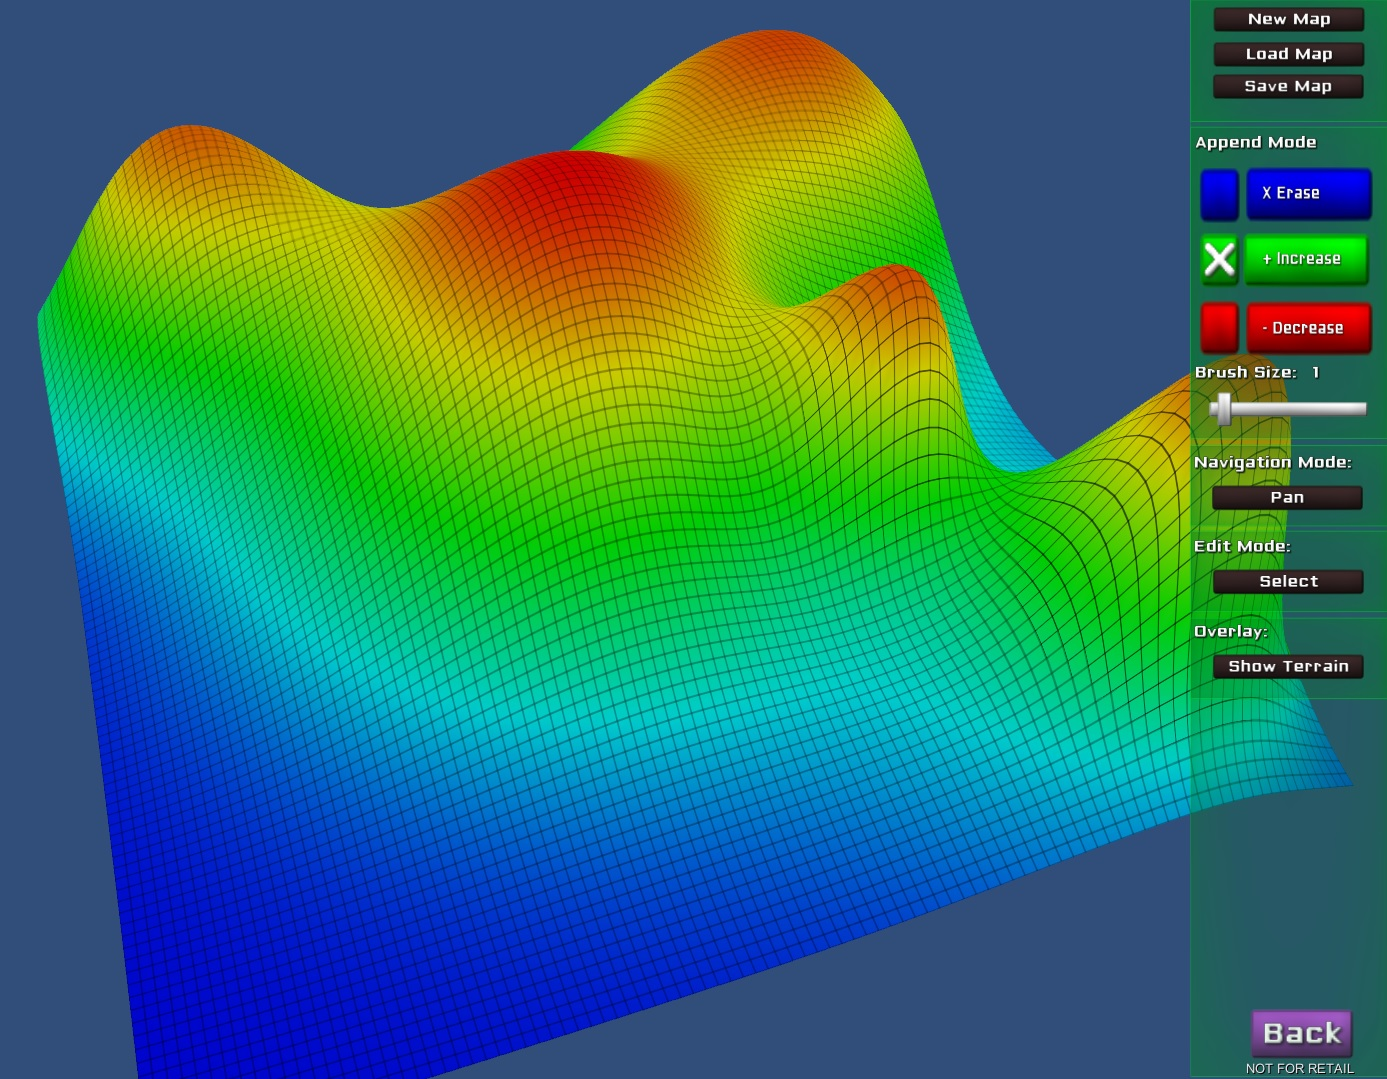
\includegraphics[width=2.8in]{DistEditExample.jpg}
	\caption{An example probability distribution map generated using the DistEdit tool.}
	\label{DistEditExample}
	\end{minipage}
&
	\begin{minipage}{0.45\textwidth}
	\centering
	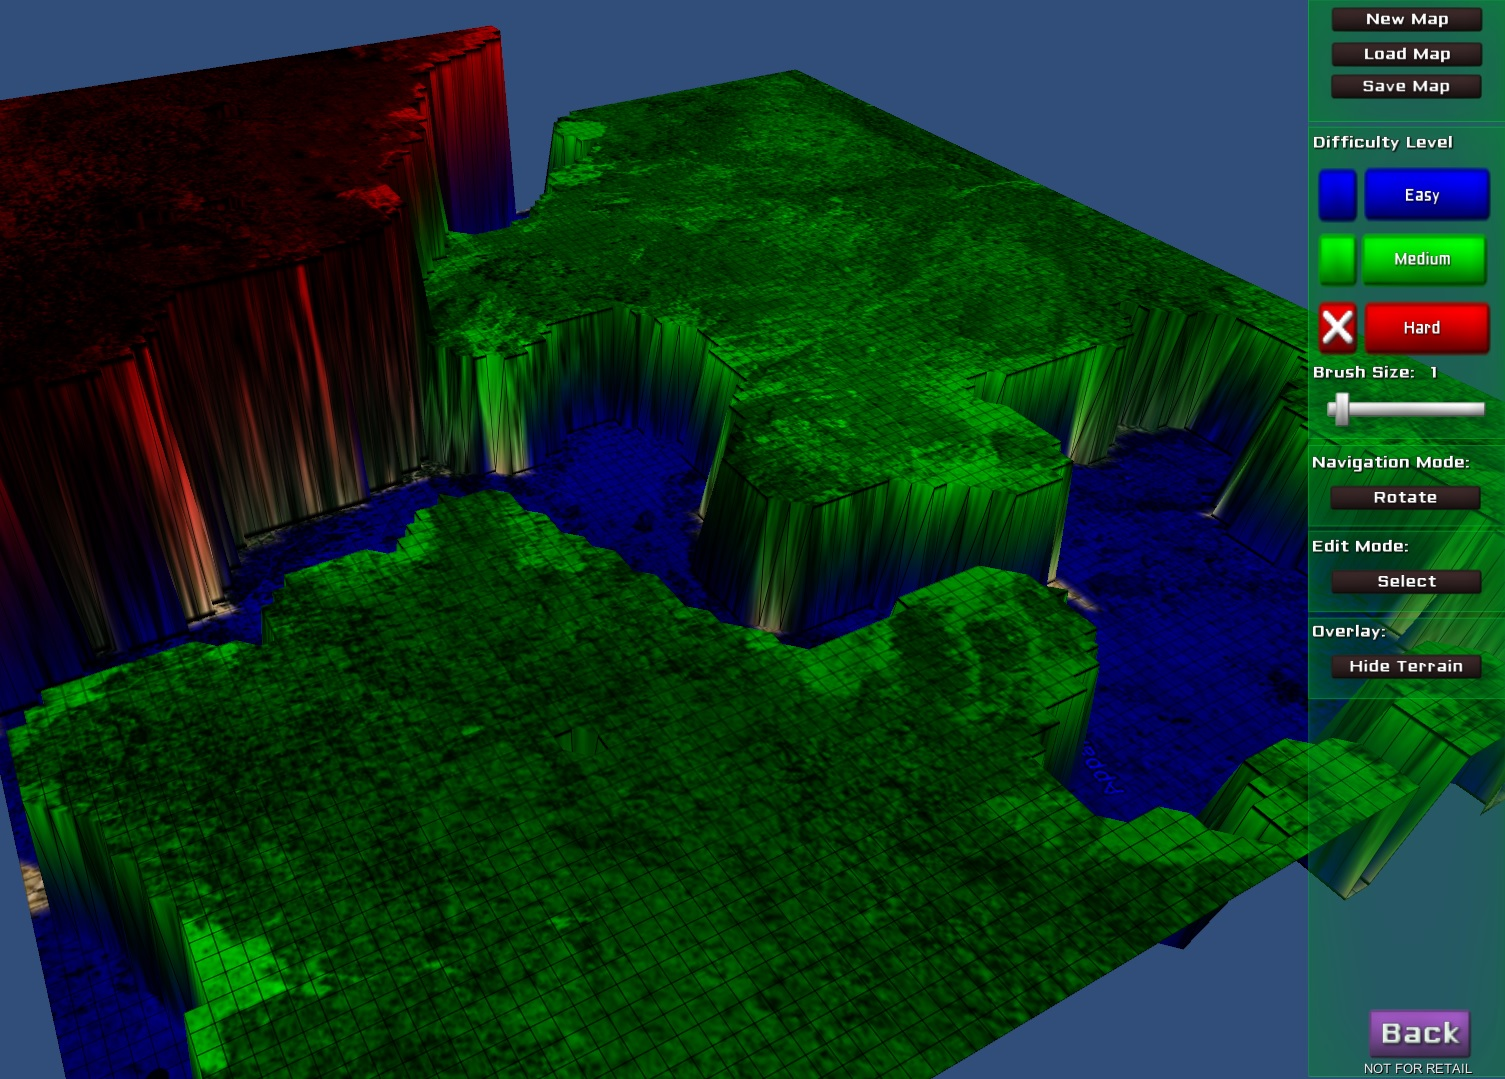
\includegraphics[width=2.8in]{DiffEditExample.jpg}
	\caption{An example task-difficulty map generated using the DiffEdit tool with a satellite image of the search region overlaid on top.}
	\label{DiffEditExample}
	\end{minipage}
\end{tabular}
\end{figure}

Searchers can use the \textbf{DistEdit} tool to modify a probability distribution map and use the \textbf{DiffEdit} tool to modify a task-difficulty map generated at the \textbf{strategic} scale. Both tools enable the user to view maps as 3D surfaces where a color map is applied for better distinction (red means high probability area or high task-difficulty level and blue means low vise versa). The user can use mouse and finger gestures to rotate/pan/zoom the respective map and edit the shapes of the maps in 3D to incorporate information that the autonomous components are unable to interpret. The user also has the option to overlay a satellite image of the search area on top of the maps for better alignment.

In \textbf{DistEdit} the user can paint Gaussian distributions onto the probability distribution map (in the form of a 3D surface) with a paintbrush tool to specify \textit{areas of focus}. The mouse click (or finger press gesture) position determines the mean of the Gaussian distribution; brush size determines the standard deviation (with a radius equivalent to three times the standard deviation); and the duration of the click (or finger press gesture) determines the scale of the Gaussian distribution. Using this tool the user can add or subtract Gaussian components to the map to create a mixture of Gaussians. The modified probability distribution can be used later to prioritize tasks and plan UAV paths. By marking an area as a high priority area, the searchers can indirectly manipulate the UAV to search the area before other areas without the need to manually specify waypoints. Figure~\ref{DistEditExample} shows an example probability distribution map generated using the \textbf{DistEdit} tool.

In \textbf{DiffEdit} the user can specify \textit{task difficulty} by using a paintbrush tool to paint on the task-difficulty map with scribbles. The user can also use a lasso tool to specify a region of irregular shape and then mark the region with selected task-difficulty level. By marking an area as a difficult area, the user can indirectly tell the UAV to make multiple passes over these areas to search more thoroughly. Figure~\ref{DiffEditExample} shows an example task-difficulty map generated using the \textbf{DiffEdit} tool with the satellite image of the search region overlaid on top.

If the user does not like the probability distribution map or task-difficulty map generated at the \textbf{strategic} scale, he or she can also use the \textbf{DistEdit} and \textbf{DiffEdit} tools to create new maps from scratch. Both tools enable the searchers to add additional information (especially the type of information autonomous components cannot interpret) to the intelligent system, relying on UAV path-planning to use the information to search more efficiently.

%===================================================
\subsection{At the Within-Episode Scale}

At the within-episode scale, given a probability distribution map marking likely places to find the missing person and a task-difficulty map indicating sensor detection probability in relationship to the spatial representation of the search area, efficient UAV flight paths need to be created quickly to support WiSAR operations. We have designed multiple path planning algorithms~\cite{Lin2009UAV,Lin2014Hierarchical} so given a starting point, (optionally) an ending point, and a desired flight duration, the Intelligent Path Planning Algorithms (IPPA) can generate flight paths that approximate the optimal path (see Figure~\ref{path} for an example) to maximize the probability of finding the missing person.

\begin{figure}
\centering
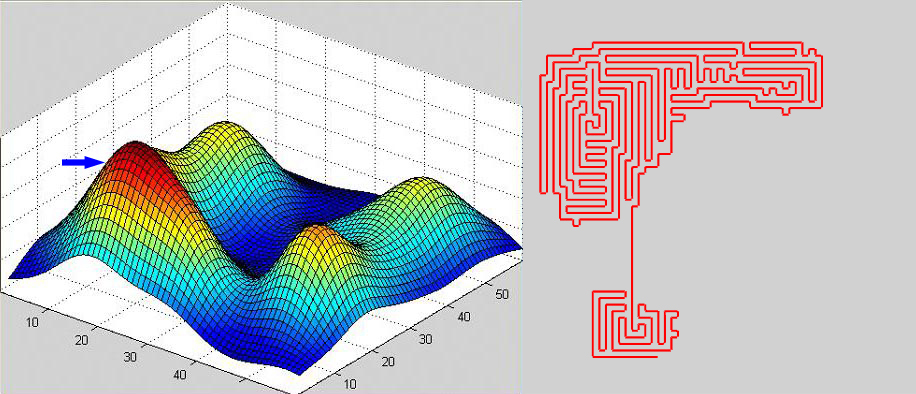
\includegraphics[width=6in]{ComplexMap.jpg}
\caption{Example UAV path generated for a complex multi-model distribution by a path planning algorithm. (The blue arrow indicates the starting point.)}
\label{path}
\end{figure}

We present in~\cite{Lin2009UAV} (Chapter~\ref{chap:IROS2009} of the dissertation) multiple intelligent path planning algorithms using Local-Hill Climbing, Potential Field, lawnmower patterns, and Evolutionary Algorithm techniques. We evaluate the performance of these algorithms against simple and complicated synthetic scenarios with the assumption of 100\% detection probability (no task-difficulty map is used). Then in~\cite{Lin2014Hierarchical} (Chapter~\ref{chap:SMCB2014} of the dissertation) we extended these algorithms to support partial detection by introducing the task-difficulty map, and also present two new (Top2 and TopN) algorithms, which utilize the \textit{Mode Goodness Ratio} heuristic we designed and enable a hierarchical search in the parameter space. We compare the performance of these algorithms against Bourgault's Algorithm~\cite{Bourgault2006Optimal} and the LHC-GW-CONV (which we present in Chapter~\ref{chap:IROS2009} and~\cite{Lin2009UAV} algorithm using three real WiSAR scenarios, and the Top2 and TopN algorithms outperformed both algorithms. To improve computation time of these algorithms, we implemented hierarchical coarse-to-fine search and hierarchical desicion making. Algorithms were also parallelized to take advantage of multi-core processor capabilities. More details of these techniques can be found in Appendix~\ref{chap:hierarchical}.

When new evidence is gathered (from UAV aerial imagery or from ground searchers) while the UAV is flying, the search plan might need to be changed in real-time. At this within-episode scale, the information management tools \textbf{DistEdit} and \textbf{DiffEdit} previously proposed can still be used to update the probability distribution and the task-difficulty maps. This provides flexibility in autonomy management. Additionally, we have designed an autonomy management interface, \textbf{SlidingAutonomy}, that enables the user to prioritize search regions and manage the desired amount of the autonomous local search along two new dimensions: changing the desired flight duration (temporal control) and adding constraints (endpoints, spatial control).

The \textbf{SlidingAutonomy} tool allows a searcher to specify a starting point and (optionally) an ending point on the terrain satellite image overlay. Then, by moving a slider, the user can control how much flight time is granted, and the IPPA algorithms generate UAV paths within the local region. Beginning from the ending point of the previous flight path segment, the searcher can plan the next path segment in the next search region. This way, the searcher can specify the order of different search regions and let the algorithm determine what paths the UAV should follow at each region. By setting flight duration and adding constraints, the searcher tells the UAV information about search priorities and at the same time, indirectly manages the local path planning based on his/her own judgment of how much the UAV can be trusted to cover a given area well. This autonomy management tool gives the user the flexibility of controlling the amount of autonomy desired without the burden of creating the entire flight path manually through waypoints. Figure~\ref{SlidingAutonomy} shows an example path depicting prioritized search regions and local paths. As the user moves the slider in the \textbf{SlidingAutonomy} tool, the system provide immediate visual feedback of what local path the system generates. This way, the searcher can easily infer the causal relationship between his/her actions (changes in flight duration) and the autonomous behaviors of the system (what path is generated). 

\begin{figure}
\centering
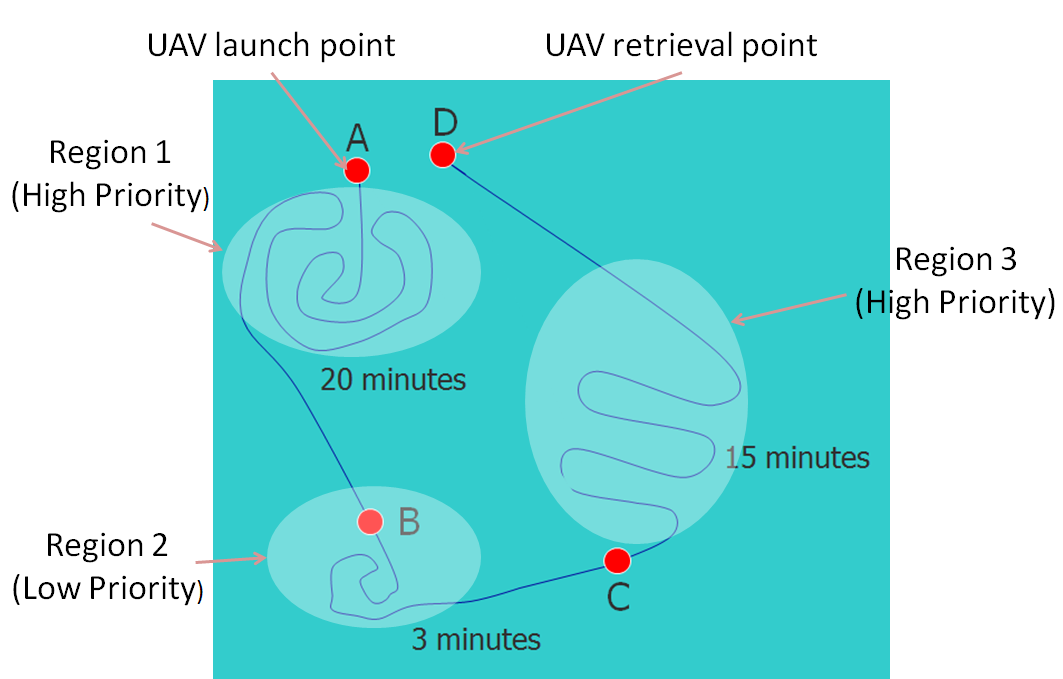
\includegraphics[width=6in]{SlidingAutonomyE.png}
\caption[An example scenario of path planning using sliding autonomy]{An example scenario of path planning using sliding autonomy: The UAV is launched at point A. Because region 1 is a high priority area, the searcher lets the UAV search for 20 minutes before arriving at point B, resulting in a longer flight path. Region 2 has low priority, so the searcher only gives the UAV 3 minutes before sending the UAV to point C, resulting in a short flight path. Region 3 is a high priority area, so the searcher gives the UAV 15 minutes. But the UAV also needs to reach Point D, the UAV retrieval point, at the end of the allocated 15 minutes. A medium length flight path is generated to meet the requirements.}
\label{SlidingAutonomy}
\end{figure}

We performed a user study to validate the usefulness of the approach. Experiment results show that the human-autonomy team outperforms human or autonomy working alone, reduces the human's cognitive workload, and improves the human experience in the human-autonomy interaction (Chapter~\ref{chap:JHRI2014} of the dissertation).


%=====================================================================================================
\section{Dissertation Chapters}

This dissertation consists of five papers, two of which are under review. This section gives a brief description of each chapter.

Chapter~\ref{chap:intro} gives an overview of our proposed autonomy management approach and provides an overall related literature review with respect to autonomy management approaches and path planning for UAV in the context of Wilderness Search and Rescue. It explains how all the components in our dissertation fit in the hierarchical structure and how they related to chapters of this dissertation.

Chapter~\ref{chap:AAAI2010}, which was published in~\cite{Lin2010Supporting}, presents autonomy integration guidelines we identified (see Figure~\ref{challenges}) when integrating UAV autonomy to the WiSAR system. We summarize the challenges along two dimensions: \textit{attributes of an intelligent system} (capability, information management, performance evaluation) and \textit{scale} (individual vs. group). The table was extended later (in Chapter~\ref{chap:JHRI2014}) to include a row for collaborative agents when a human agent works together with the autonomous agent. The paper emphasizes on how information management is an important attribute of an intelligent system, where users assign tasks to autonomous algorithms by matching capabilities of the autonomous agents based on information fusion from the overall distributed system. It also describes in detail how the UAV path planning problem fits in the overall intelligent system of using UAVs to support Wilderness Search and Rescue.

Chapter~\ref{chap:CMOT2010}, which was published in~\cite{Lin2010Bayesian}, presents a Bayesian model that uses publicly available terrain features data to help model lost-person behaviors. This approach enables domain experts to encode uncertainty in their prior estimations and also makes it possible to incorporate human behavior data collected in the form of posterior distributions. It also enables the searcher to influence the probability distribution map generated by changing prior beliefs in the transitional probabilities between terrain features and by selecting what subset of past human behavior data to feed to the model.

Chapter~\ref{chap:IROS2009}, which was published in~\cite{Lin2009UAV}, explores several path planning algorithms (with and without set destination) and describe some novel techniques in solving the problem of maximizing sensor (UAV onboard video camera) coverage within a set time to support Wilderness Search and Rescue. The task-difficulty map is not used and we assume 100\% detection probability. Performance of these algorithms are compared against typical WiSAR scenarios, and experiment results show that these algorithms yield high quality solutions that approximate the optimal solution.

Chapter~\ref{chap:SMCB2014}, which is under review in~\cite{Lin2014Hierarchical}, proposes a heuristic, \textit{Mode Goodness Ratio}, which uses a Gaussian Mixture Model to prioritize search subregions, and presents two path planning algorithms (Top2 and TopN) that utilize the heuristic and hierarchically search for effective paths through the parameter space at different levels of resolution. Performance of the new algorithms are compared against two published algorithms in simulated searches with three real search and rescue scenarios where both the probability distribution map and the task-difficulty map are used. Results show that the new algorithms outperform existing algorithms significantly when partial detection is considered, and can yield efficient paths that yield payoffs near the optimal. 

Chapter~\ref{chap:JHRI2014}, which is in preparation to be submitted to \textit{Journal of Human-Robot Interaction}, extends the autonomy integration guidelines we identified in Chapter~\ref{chap:AAAI2010} to include collaborative agents when a human agent works together with the autonomous agent. It proposes two additional dimensions for autonomy management: time allocation (temporal) and constraints (spatial), and presents a new autonomy management approach named \textbf{Sliding Autonomy} where the human agent in the human-autonomy team can assign different flight duration to the path planning algorithms to plan path segments and use endpoints to manage search region priorities. A user study was performed to validate the usefulness of the approach. Experiment results show that this approach enables the human-autonomy team to outperform human or autonomy working alone, reduces the human's cognitive workload, and improves the human experience in the human-autonomy interaction.

In Chapter~\ref{chap:MapEdit} we describe the \textbf{DistEdit} and \textbf{DiffEdit} tools at the \textbf{between-episodes} scale in detail, and demonstrate how the \textit{probability distribution map} and the \textit{task-difficulty map} generated at the \textbf{strategic} scale can be modified using mouse and finger gestures to incorporation additional information. The two tools can also create maps from scratch.

Chapter~\ref{chap:Conclusions} concludes findings of the dissertation work and summarizes the contribution of the dissertation. 
We also describe possible future work to extend the research at the three distinctive scales we proposed for our autonomy management approach.

In appendix~\ref{chap:complexity} we present the complexity analysis of the UAV path planning problem and why a heuristic approach is preferred to both dynamic programming and reinforcement learning approaches. Appendix~\ref{chap:result} presents the full experiment results for Chapter~\ref{chap:SMCB2014}. Appendix~\ref{chap:hierarchical} describes how hierarchical desicion making and hierarchical coarse-to-fine search techniques are used in algorithm design. Appendix~\ref{chap:modes} explains the algorithm to identify modes on a 3D surface, which is used in our Top2 and TopN algorithms.
\chapter[Paper: Supporting Wilderness Search and Rescue with Integrated Intelligence: Autonomy and Information at the Right Time and the Right Place]{Paper: Supporting Wilderness Search and Rescue with Integrated Intelligence: Autonomy and Information at the Right Time and the Right Place\footnote {Published in Twenty-Fourth AAAI 2010 (Association for the Advancement of Artificial Intelligence) conference. Authors are Lanny Lin, Michael Roscheck, Michael A. Goodrich, and Bryan S. Morse.}}
\label{chap:AAAI2010}

%=================================================================================
\begin{abstract}
%\begin{quote}
Current practice in Wilderness Search and Rescue (WiSAR) is analogous to an intelligent system designed to gather and analyze information to find missing persons in remote areas. The system consists of multiple parts --- various tools for information management (maps, GPS, etc) distributed across personnel with different skills and responsibilities. Introducing a camera-equipped mini-UAV into this task requires autonomy and information technology that itself is an integrated intelligent system to be used by a sub-team that must be integrated into the overall intelligent system. In this paper, we identify key elements of the integration challenges along two dimensions: (a) \textit{attributes of intelligent system} and (b) \textit{scale}, meaning individual or group. We then present component technology that offload or supplement many responsibilities to autonomous systems, and finally describe how autonomy and information are integrated into user interfaces to better support distributed search across time and space. The integrated system was demoed for Utah County Search and Rescue personnel. A real searcher flew the UAV after minimal training and successfully located the simulated missing person in a wilderness area.
%\end{quote}
\end{abstract}


%=================================================================================
\section{Introduction}
Wilderness Search and Rescue (WiSAR) can be thought of as an intelligent system designed to gather and analyze information to find and assist humans who are lost or injured in remote areas such as deserts and mountains. The system consists of multiple parts --- various tools for information management (maps, GPS, etc) distributed across personnel who have different skills. Using a camera-equipped mini-Unmanned Aerial Vehicle (UAV) to aid search can provide aerial imagery of a search area with the benefits of quick coverage of large areas, access of hard-to-reach areas, and lower cost than manned aircraft. 

Introducing a UAV into the WiSAR system requires autonomy and information technology that itself is an integrated intelligent system to be used by a WiSAR sub-team, and this sub-team and associated technology must be integrated into the overall intelligent system. This integration inevitably creates the need for new roles and responsibilities in order to manage the UAV and the aerial imagery~\cite{Adams2009Cognitive,Goodrich2007Using}. The task of creating a useful technology for supporting these roles is to make sure that these responsibilities are performed by appropriate people at an appropriate time with a satisfactory level of performance. Doing this requires the creation of algorithms that efficiently offload portions of responsibility to autonomous algorithms, creating an intelligent distributed system that facilitates the coordination and information management among roles. The need for efficiency creates the need to monitor and evaluate the performance of the system as a whole.

\begin{table}
\footnotesize
	\begin{center}
		\begin{tabular}{|p{3.4cm}|p{2cm}|p{4cm}|p{5cm}|}
			\hline
			 & \textbf{Capability} & \textbf{Information} & \textbf{Performance} \\
			 &  & \textbf{Management} & \textbf{Evaluation} \\
			 \hline
			 \rr \textbf{Intelligence of individual tools} & Autonomy & Flexibility & Progress toward individual goal \tn
			 \hline
			 \rr \textbf{Intelligence of distributed system} & Modularity & Fusion (Communication) & Collective progress/quality \tn
			\hline
		\end{tabular}
	\end{center}
\caption[Autonomy integration challenges]{Integration challenges defined along two dimensions. Horizontal dimension: attributes of intelligence. Vertical dimension: scale.}
\label{dimensions}
%\vspace*{-3ex}
\end{table}

In this paper we describe our efforts in developing autonomous algorithms and user interfaces that integrate components of machine and human intelligence with the goal of making UAV technology useful to real searchers in WiSAR. 
Thus, this paper is consistent with Drucker's definition of automation as a ``concept of the organization of work~\cite{Drucker2006Practice}.'' 
Intelligently organizing work requires that we identify key elements of the integration challenges organized along two dimensions: \textit{attributes of an intelligent system} (capability, information, performance evaluation) and \textit{scale} (individual versus group); see Table~\ref{dimensions}. We then present component algorithms  that augment or supplement search responsibilities. Next we describe how autonomy and information are integrated into user interfaces to better support distributed coordination of multiple searcher roles across time and space with respect to the integration challenges we identified.
%Then we use see-ability metrics to evaluate performances.

Validating an integrated system is always difficult. The goal of our research is to develop technology that provides help to real searchers; therefore, we believe a good way to validate our integrated system is to put it through a test in a real-world environment in front of real users. We summarize the experience of a recent field demo for Utah County Search and Rescue team representatives, where a real searcher acted as the UAV operator in a simulated search and rescue mission after minimal training.



%=================================================================================	
\section{Related Work}

The goal of our research is to support fielded missions in the spirit of Murphy's work~\cite{Casper2003Human}. UAV technology has emerged as a promising tool in supporting WiSAR~\cite{Bourgault2003Coordinated,Murphy2008Cooperative}. The UAV technology is an intelligent system with the integration of many component autonomous algorithms and user interfaces (related work for these components are referenced in their relative sections). Integration at this level requires tremendous effort. For example, building robots (GRACE and Spartacus) that are capable of attending a conference~\cite{Simmons2003Grace,Michaud2007Spartacus} required the integration of many technologies (e.g., localization/navigation, gesture/face recognition, and speech recognition/generation) and multiple modalities (e.g., mobility, vision, audition, and reasoning).

To integrate the UAV intelligent system into existing WiSAR practices --- which we argue is an intelligent system by itself~\cite{Setnicka1980Wilderness} --- creates additional challenges. Salas and Fiore~\shortcite{Salas2004Team} provide great insights on challenges across people and machines, and across time and space in distributed teams. Sycara and Lewis~\shortcite{Sycara2002Integrating} also asked the questions: 1) can a software agent perform the task? and 2) can the agent's assistance contribute toward team performance? Tso et al.\ ~\shortcite{Tso1999Multi} identified that integrating a UAV into the search task creates at least two roles: a pilot that controls the UAV and a sensor operator that analyzes the sensor outputs, and lessons from other search-related domains~\cite{Drury2003Awareness} show that multiple roles are required and these roles can be supported by autonomy algorithms and user interface technologies. These findings motivate and guide our research in developing UAV technology to support WiSAR operations.


\begin{figure}
\centering
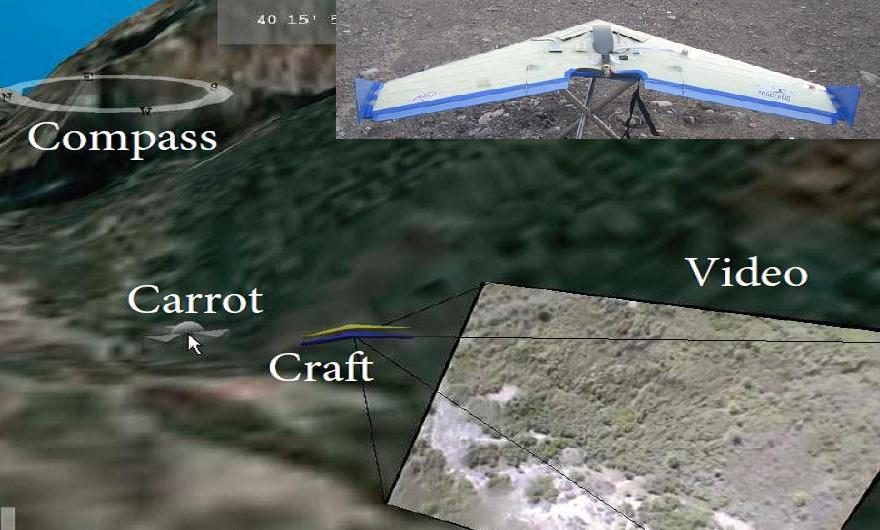
\includegraphics[width=6.0in]{UAVCarrot.jpg}
\caption[A screenshot of the UAV operator interface]{A screenshot of the UAV operator interface showing the position/orientation of the UAV, the orientation of the camera, and the projected video. (Top right: The UAV used in our research.)}
\label{UAVCarrot}
%\vspace*{-3ex}
\end{figure}


%=================================================================================	
\section{UAV Overview}

UAVs used in our research have wingspans of 42-50 inches, weigh approximately 2 lbs, and use lithium battery-powered propellers (see Figure~\ref{UAVCarrot}a). The airframes are designed so each UAV can stay aloft for up to two hours and travel at approximately 12-15 meters per second. The onboard sensors include three-axis rate gyroscopes, three-axis accelerometers, static and differential barometric pressure sensors, a GPS module, and a video camera on a gimbaled mount. An autopilot, designed by the BYU MAGICC lab~\cite{Beard2005Autonomous}, enables roll and pitch angle stabilization, attitude stabilization, altitude control, and waypoint following. The UAV uses a 900 MHz radio transceiver for data communication and an analog 2.4 GHz transmitter for video downlink. The typical operating height above ground is 60--100 meters so the UAV can avoid trees and slight terrain variations while still provide enough resolution so a human form can be discerned in the video~\cite{Goodrich2008Supporting}.

%=================================================================================	
\section{Integration Challenges}

We organize integration challenges along two dimensions: attributes (capability, information management, and performance evaluation) and scale (individual tool vs distributed system), as shown in Table~\ref{dimensions}. We assert that an intelligent system should display several attributes associated with intelligence across multiple scales. Capability pertains to the identification and development of specialized behaviors. Information management focuses on how information is presented, handled, and shared. Performance evaluation deals with monitoring the health of the system or progress toward the intended task goal. In this section we use this taxonomy to describe components of the UAV technology in the context of WiSAR. 

The individual tools were designed partly in response to a cognitive task analysis conducted on the WiSAR domain to inform the design of UAV technology~\cite{Adams2009Cognitive}.
 
The analysis identified four primary search tactics used in WiSAR: \textit{hasty search}, \textit{constrained search}, \textit{high priority search}, and \textit{exhaustive search}. Also, observations from several user studies~\cite{Cooper2008Towards} show that the best perspective (e.g., chase, north-up) for detecting and localizing a target depends on the type of search and the type of distribution (likely places to find the missing person). These findings suggest that multiple control modes, path planning methods, and perspectives are needed to support various search tactics and scenarios. These are examples of the capability for \textit{individual tools}. Since autonomous algorithms can replace or supplement searcher responsibilities, a wide range of capability is desired.

%Integrating a UAV into the search task creates at least two roles: a pilot that controls the UAV and a sensor operator that analyze the sensor outputs~\cite{tso1999multi}. The roles are really just groupings of responsibilities associated with intelligently using an airborne camera. The task of creating a useful technology for supporting these roles is to make sure that these responsibilities are performed by appropriate people at an appropriate time with a satisfactory level of performance. 
For the WiSAR system, the cognitive task analysis also identified two key WiSAR subsystems; information acquisition and information analysis. Combining this result with observations from past field trials, we see four roles emerge when a UAV is integrated into the search~\cite{Goodrich2008Supporting}. \textit{UAV operator}: responsible for guiding the UAV and the gimbaled camera to various locations and monitoring the UAV; \textit{video analyst}: responsible for scanning and analyzing imagery to detect potential clues; \textit{mission manager}: responsible for managing the search and prioritizing efforts based on information obtained; \textit{ground searcher}: (when supporting the UAV) responsible for investigating potential clues found in aerial imagery. Each role consists of a grouping of responsibilities. The task of creating useful technology for supporting these distributed roles is to make sure that these responsibilities are performed by appropriate people at an appropriate time with a satisfactory level of performance. Since people may take on (partial) responsibilities of other roles, the video analyst and the UAV operator might share responsibilities, these behaviors suggest that capabilities of individual systems should be modular to mix and match across roles. \textbf{Modularity} is a requirement for an intelligent distributed system -- it is the adaptable chunking of responsibility and capability.

\textbf{Flexibility}, in information management, is the ability to appropriately match capability to task according to the information available to the operator.
%For the HRI, this means that we have a usable interface that promotes situation awareness and allows a human to easily task autonomy.
The cognitive task analysis indicated that WiSAR search is an iterative process of gathering, analyzing evidence and planning for gathering more evidence, where probability refinement plays an important part during search. The analysis also identified that searches require considerable human judgment, especially as new evidence is collected. These findings suggest that tools and autonomy need to be flexible so they can be interrupted, temporarily aborted, and possibly resumed later. For example, if an object is spotted in the video, the UAV operator stops the current flight pattern and loiters around the Point Of Interest (POI) to gather more information. Once the UAV operator aborts the loiter mode, the UAV automatically resumes the previous flight pattern to continue to gather information.

For a distributed system, Information \textbf{Fusion} is an important element that efficiently combines and presents information from various sources to a user and also shares information among multiple users. For example, the user interface for the UAV operator includes the terrain map, an icon indicating the position and attitude of the UAV, an integrated video feed projected onto the terrain map showing the direction of the gimbaled camera, and various meters showing UAV status (e.g., speed, altitude, battery life); see Figure~\ref{UAVCarrot}. Another example is a video analyst helping to annotate clues in video imagery, and communicating the data to the mission manager who can update the search plan accordingly.

For each individual tool, the ability to evaluate the quality and the progress toward the individual goal can be useful and represents the importance of performance evaluation. A coverage map, for example, improves the UAV operator's situation awareness of how well an area has been covered. Morse et al.~\cite{Morse2010UAV} defined two see-ability metrics (described in the See-ability section). An \textit{instantaneous see-ability} evaluation helps the video analyst get a sense of the quality of a single frame of video. As for the distributed system, an overall, or group quality evaluation is more appropriate. A mission manager might want to know the \textit{collective see-ability} to understand how well the terrain is seen by all frames of video or combined coverage of the UAV and ground searchers.

In the following three sections we match components of our UAV system to the three attributes (columns) of our intelligent system taxonomy and show how they support various searcher roles at the right time and the right place.



%=================================================================================	
\section{Autonomy Components}

This section presents a wide breadth of \textbf{autonomy} components currently in place to support searcher roles and responsibilities. They map to the \textbf{Capability} column in our taxonomy (Table~\ref{dimensions}). The \textbf{modular} design allows mix and match of autonomy components to support the distributed system. Here we use the term ``low-level autonomy'' to describe components that only involve simple math calculations in contrast to the term ``advanced autonomy,'' where complex algorithms and interrelationships are required.

%==================================================
\subsection{Low-Level Autonomy}

%=============================
\subsubsection{Autopilot:} Pitch/roll/yaw and altitude stabilization, attitude controls, and waypoint following.
\subsubsection{Deploy and retrieve:} Two auto launch modes (take off to waypoint, spiral take off) and two auto land modes (rally land, deep stall).
\subsubsection{Gimbaled camera control:} A point can be set on the terrain map so the gimbaled camera constantly aims at the point independent of the UAV's flight path.
\subsubsection{Path planning:} Simple flight patterns include spiral, lawnmowing, and Zamboni.
\subsubsection{Safety:} If no waypoint is set or after reaching the end of set path, the UAV loiters around last waypoint. If the UAV loses communication with the base, it automatically returns to base and loiters.

\begin{figure}
\centering
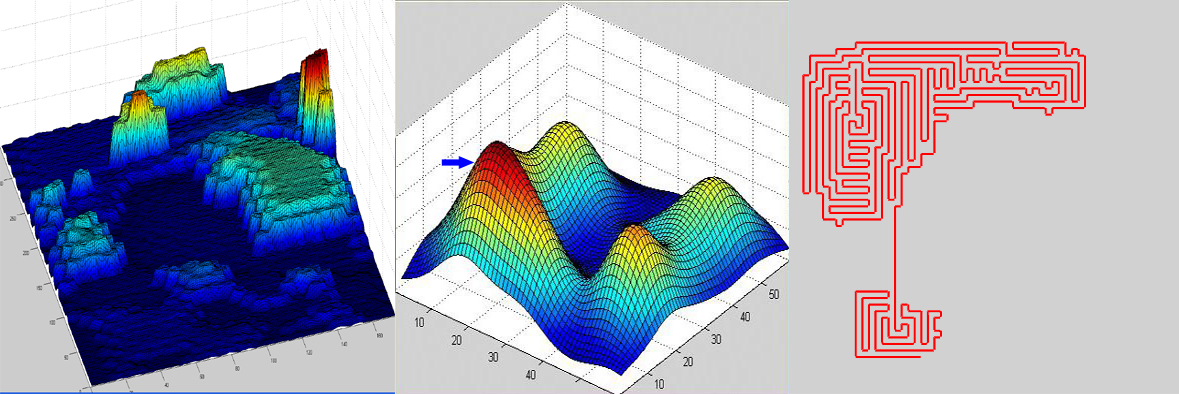
\includegraphics[width=6.0in]{maps.jpg}
\caption[Example posterior distributions and an algorithm-generated path]{Left: a posterior predictive distribution at 200th time step generated using the Bayesian model. Middle: a multimodal distribution used to test path planning (arrow marks starting point). Right: path generated using Intelligent Path Planning.}
\label{pathplanning}
%\vspace*{-3ex}
\end{figure}

%==================================================
\subsection{Advanced Autonomy}
%=============================
\subsubsection{Distribution Generation:}
A Bayesian model that incorporates past human behavior data and publicly available terrain data (topography, vegetation, and elevation) is used to automatically generate a posterior predictive distribution of the likely places of finding the missing person~\cite{Lin2009Bayesian}. The Markov chain Monte Carlo Metropolis-Hastings algorithm generates a temporal distribution showing how the distribution changes over time (Figure~\ref{pathplanning}). Given enough time, the distribution converges to a static state. The resulting distribution can be used by the search manager to prioritize search resources and develop search plans. It can also be used by the UAV operator for automatic path planning to maximize accumulated probability for a fixed flight duration.


%=============================
\subsubsection{Path planning:}
Two advanced path planning algorithms are described here: \textit{Generalized Contour Search}~\cite{Goodrich2008Supporting} and \textit{Intelligent Path Planning}~\cite{Lin2009UAV}. The ability to control the gimbaled camera to aim at a target point while orbiting enables a \textit{Generalized Contour Search} path planning algorithm. A queue of target points that follow the contours of the distribution of the missing person's likely locations can be created from which the algorithm interpolates (bicubic interpolation) and resamples at uniform distances. Lawnmower and spiral paths naturally emerge from the algorithm for uniform and Gaussian distributions respectively, and they are the optimal paths. It is also possible to use the algorithm to follow the contours of steep terrain by aiming the camera out the side of the UAV. The second path planning algorithm aims to maximize the accumulated probability for the path generated given a distribution, a starting point (optionally an ending point), and desired flight time. The camera footprint traverses a grid of probability nodes (enabled by the gimbaled camera) while the UAV approximates the path generated. Near optimal flight paths are generated using an evolutionary approach, where seed paths are generated using various hill-climbing and potential fields algorithms. Simulation results show the algorithm works well with a variety of probability distributions, including complicated multi-modal distributions (Figure~\ref{pathplanning}). These advanced algorithms enrich the autonomy tool set for the UAV operator and can potentially be useful for the \textit{high priority search} and \textit{exhaustive search} techniques when systematic coverage is desired.


%=============================
\subsubsection{Video mosaicing:}
The term \textit{mosaic} means to ``stitch'' together multiple frames of video of a static scene from a moving camera~\cite{Szeliski2006Image}. A real-time \textit{temporally local mosaic} technique~\cite{Morse2008Application} was developed using Harris corner detector to identify feature points and then using RANSAC~\cite{Fischler1981Random} to estimate the Euclidean transformation between each pair of frames. User studies using simulations and experience from field trials show that small mosaics of only the last few seconds of video is sufficient to provide both increased opportunity for detection and increased sense of relative spatial relationships. Figure~\ref{mosaic} shows an example of the local mosaic view where the same object is only visible in a few frames in original video but is visible for nearly one hundred frames using the technique.

\begin{figure}
\centering
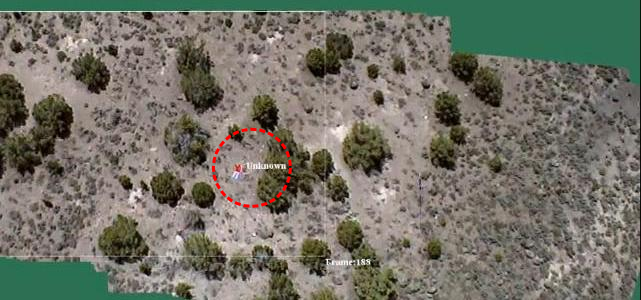
\includegraphics[width=6.0in]{mosaic.png}
\caption[Example of a video mosaic with an annotation]{Example of a video mosaic with an annotation (indicated by a red circle).}
\label{mosaic}
%\vspace*{-3ex}
\end{figure}


%=============================
\subsubsection{Anomaly detection (under development):}
A color anomaly detection algorithm is currently under development that adapts hyperspectral anomaly detection methods to find man-made objects in wilderness scenes. This algorithm adds another autonomy capability to the tool set and can recommend points of interest in the video imagery to the video analyst, potentially reducing mental workload. We mention this component in this paper for completeness.

%\begin{figure}
%\centering
%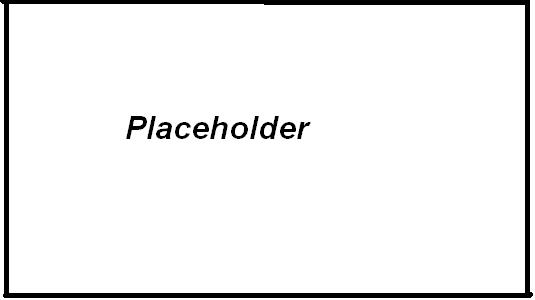
\includegraphics[width=3in]{Placeholder.jpg}
%\caption{Group of pictures showing GUI}
%\label{GUI}
%%\vspace*{-2ex}
%\end{figure}


%=================================================================================	
\section{User Interfaces}

In this section we describe the user interfaces developed to support various searcher roles with a focus on explaining how we integrate autonomy components (including control modes) and human intelligence. Interface techniques provides control \textbf{flexibility} with current information state, and information sharing and \textbf{fusion} improves the efficiency of the overall distributed system. They map to the \textbf{Information Management} column in our taxonomy (Table~\ref{dimensions}).

The UAV software consists of several components. \textbf{Phairwell} is the \textit{augmented virtuality} interface used to ``fly'' the UAV (see Figure~\ref{UAVCarrot}). The \textbf{Wonder Server} consists of central management software for capturing, storing, and retrieving video, UAV telemetry, annotations, and other related information. Finally, the \textbf{Wonder Client} is the GUI used by the video analyst and mission manager and provides video mosaic and annotation capabilities. Video and telemetry data are streamed from the Wonder Server.

%Control gimbaled camera separately from UAV path
%Various flying mode:
%- Manual 
%- Carrot and stick
%- Patterns
%- Contour following
%Break out of planned path and resume path afterwards


%=============================
%\vspace*{4 pt}
\noindent\textbf{Phairwell for UAV Operator:}
The UAV operator's main responsibilities include assigning the UAV a specific task, ensuring that it is properly performing that task while monitoring the UAV's ``health and safety,'' monitoring the live video, and interacting with the UAV when needed (e.g., once the video analyst spots a suspicious object, a change in the plan is made, or when the UAV needs attention). 

% Although the UAV has a high level of autonomy, another level of autonomy is used underneath Phairwell to manage things the UAV cannot. Since the UAV operator is provided with a vast range of autonomies, a high level of human intelligence is required to understand and select the right autonomies for each situation. In this section, we describe the different types of machine intelligence (autonomies) that are available to the operator.  

%HAG and automated altitude gain:
%It is important for the UAV to maintain a low, but safe, height above ground (HAG) so that objects in the video are large enough to be seen. However, the UAV is only aware of its current altitude and not the terrain around it. It would be a difficult and laborious task for the UAV operator to continually watch and adjust the UAV's altitude, especially with the rough terrain typical of WiSAR settings. This task is an ideal candidate for autonomy, completely freeing the operator of this responsibility. Phairwell continually monitors the geo-referenced terrain model simulation and looks forward in time along the UAVs flight path and instructs the UAV to adjust its altitude to maintain a consistent HAG.

%Flight modes and waypoints: 
Phairwell supports four flight modes while searching: \textit{manual}, \textit{carrot and camera}, \textit{flight plan}, and \textit{loiter now}. These modes represent autonomous behaviors that help the UAV operator efficiently assist the video analyst. \textit{Manual} mode commands the UAV to match a course and altitude set using the arrow keys. \textit{Carrot and camera} allows the operator to direct the UAV and camera with the mouse. \textit{Flight plan} mode commands the UAV to fly waypoints that the operator selects manually or that are generated automatically by one or more search patterns. The \textit{loiter now} mode interrupts the UAV's current behavior so the operator or UAV team can briefly ignore the UAV.

%Camera pointing: 
While directing the UAV is important, the primary goal is to manipulate the camera efficiently to provide the video analyst with the needed video. The speed of the UAV coupled with slow user response makes it impossible for the operator to manually track specific ground objects, a commonly required task. Instead, the UAV operator can select a terrain location in Phairwell and have the UAV fix the camera on the location. The UAV autonomy can maintain this lock, even when the UAV is turning rapidly or knocked about by gusts of wind. This allows the UAV operator to easily adjust the camera according to the needs of the video analyst.

%The ability to fix the camera on a specific location while loitering or flying around it is essential when investigating a point of interest (POI) or providing aerial support for ground searchers. When the terrain is sufficiently rough or the UAV is affected by wind, this camera pointing technique is also used to provide more stable and complete video coverage by briefly fixing the camera on discretized points along the flight path.

%Phairwell provides four perspective modes~\cite{goodrich2009lessons} (in addition to free-look) that automatically adjust the virtual camera to maintain the desired perspective. These are chase, track-up, north-up, and pilot perspectives. The ``best'' perspective depends on the task and the type of situation awareness the operator needs~\cite{cooper2008combine}. The chase perspective locks the virtual camera behind and above the UAV in order to provide visual information about the UAV's status and its local environment. The track-up and north-up perspectives both show the UAV from a satellite perspective where the UAV remains at the center of the screen. Track-up orients the map so that the UAV is always facing up while north-up fixes the map so north is always up. The pilot perspective shows provides a view from perspective of the UAV's camera. The operator must select the appropriate perspective mode based on their current task.

Although the UAV's autonomy allows it to fly a predefined flight plan, the UAV operator must often interrupt the autonomy and then resume it later. Phairwell allows the UAV operator to effortlessly change control modes, perform some task, and resume the previous control mode. This capability has been used routinely when the UAV is flying a search pattern and the video analyst sees something and wants the UAV to go back and take a closer look. This specific autonomy is described more fully in the next section.


%=============================
%\vspace*{4 pt}
\noindent\textbf{Wonder Client for Video Analyst:}
The Wonder Client interface serves as the video analyst's primary tool. They have the flexibility to select between either the live video or mosaiced views. The interface also provides tools to modify the brightness, contrast, and other image properties of the live video or mosaic, which often need to be adjusted to make objects more recognizable.

The video analyst also uses the Wonder Client to annotate the video. Annotations mark objects in the video with a timestamp and user notes so that they can be found quickly in the future. An example can be seen in Figure~\ref{mosaic}. When an annotation is placed on the video mosaic, it is tied to the geo-referenced coordinates of the underlying terrain. Therefore, annotations marked on previous video frames are automatically displayed on future frames, ensuring that the video analyst does not repeatedly identify the same object while also providing an efficient means of visually tracking the object. 

The video analyst can also indicate any geo-referenced location in the video as a POI that they want to immediately return to and investigate. The system then automatically communicates this information to Phairwell, giving the UAV operator the option of letting the autonomy redirect the UAV to investigate.


%=============================
%\vspace*{4 pt}
\noindent\textbf{Wonder Client for Mission Manager:}
The mission manager is responsible for assessing what has been searched and how well. This information is then used to plan further search efforts. While assessing ground searcher coverage is a common practice, UAV-assisted search adds a new and challenging aspect to this task. A coverage map showing the quality of the search is generated from the collective see-ability estimates to provide the mission manager with a complete view of the terrain the UAV video covered.

The Wonder Client gives the mission manager access to all the video analyst's POIs and annotations. The mission manager can then review the POIs and classify them as worth investigating or not. Those that are worth investigating are prioritized and placed in a pending search queue. The mission manager then assigns the UAV-team or ground searchers to investigate these points. Once the POI is located, the findings are reported back to the mission manager for assessment. However, investigations executed by the UAV-team will lead to this whole process being repeated.


%=============================
%\vspace*{4 pt}
\noindent\textbf{For Ground Searchers (under development):}
Successful search requires that ground searches quickly and thoroughly search their assigned area. We have begun development of a system that utilizes the concept of see-ability to support ground searchers in these efforts. A portable GPS device will be used to display a see-ability map, providing a visual representation of the thoroughness and quality of their search based on what they should have seen.

Communication between ground searchers and the UAV-team has proven limited and difficult. This same portable device will be used to bridge this communication gap. For example, when a ground searcher is assigned to investigate a POI, instead of radioing the GPS coordinates, the device will automatically receive the coordinates, overlay the UAV aerial imagery with the annotations, and provide the searcher with directions to the location.

%=============================
\section{See-ability Metrics}
\label{sec:seeability}
The ``see-ability'' metric~\cite{Morse2010UAV} was developed to address the challenge of understanding the search-related quality given by UAV video. This involves two different measures: \textit{instantaneous see-ability} measures the quality of a single video frame while \textit{collective see-ability} measures the overall quality provided by all video frames. They map directly to the \textbf{Performance Evaluation} column in our taxonomy (Table~\ref{dimensions}). 

The instantaneous see-ability computation uses the semi-accurate camera's location and pose information, terrain models, satellite imagery and computer vision techniques to geo-register each frame of video. The geo-registered frame is used to estimate the resolution with which each point in the video is seen. This metric could provide information about the quality of the video coverage for the video analyst. A user study showed that there was a moderately strong correlation between the instantaneous see-ability estimates and measured detection rates~\cite{Morse2010UAV}. Collective see-ability is determined by the number of times each point has been seen, from what distance, and from which and how many different angles. This is done by combining all of the instantaneous see-ability estimates available for a single point on the terrain. This metric provides the mission manager with information about the overall quality of the entire search.

%=================================================================================	
\section{Demonstration}

We believe a good way to validate our system is to demonstrate its usability in front of real searchers in a real-world environment. In the past several years, many field trials were operated by students pretending to be searchers. A demo to real searchers focuses more on the intended intelligence of the system. That led to a field demo on November 21, 2009 for representatives of the Utah County Search and Rescue team in a remote wilderness area in Elberta, Utah.

Three searchers participated in the demo. One searcher, R, acted as the UAV operator and flew the UAV in a simulated search and rescue mission while the other two searchers observed the mission and inquired about the capabilities of the system, the system structure, and the operation protocols. Professors and students of BYU volunteered as video analysts and ground searchers. R had received 30 minutes UAV operator training and also practiced in a simulated environment for a few hours. The mission objective was to locate a simulated missing person (a dummy placed in the wilderness) as quickly as possible in a team effort (UAV operator, video analyst, and ground searchers) utilizing the UAV technology. The responsibilities of the mission manager were split between the UAV operator and the video analyst. The missing person was successfully identified in the mosaic view, and the GPS location was radioed to the ground searchers, who successfully located the missing person. The entire mission completed in under 35 minutes.

The anomaly detection autonomy component and the GUI for ground searchers were not fully implemented and, therefore, were not included in the demo. Other than the distribution generation, intelligent path planning, and see-ability metric components (implemented and validated but not fully integrated), all other technologies described in this paper were available and functional.

We conducted an in-depth interview with R several weeks after the demo. Here we share only a portion of his feedback due to space limitations. R thinks the UAV operator interface is ``very easy to pick up'' and 30 minutes of training was plenty. His reason for practicing in the simulated environment was to explore and avoid silly mistakes. A few new features were available at the demo, but he was able to learn them quickly. He liked the video feed inside the UAV operator GUI because it helped him align the map with the video. One interesting incident was that he was able to identify the simulated missing person before the video analyst, probably the result of his trained eye. He also suggested that including ruler type tools in Phairwell could help him get a better perspective of the map. Feedback from his fellow searchers included comments such as ``That was cool!'' and ``This could work!''

Another key benefit of the demo is that it raises interest from the WiSAR community on technologies that can potentially assist WiSAR operations and opens the door for more direct collaboration between the WiSAR community and academic researchers in the near future.

%=================================================================================	
\section{Conclusions and Future Work}

To make UAV technology useful for WiSAR requires the integration of an intelligent UAV system into the existing intelligent WiSAR system. The autonomy components of the UAV technology also need to be integrated to support both individual searcher roles and the distributed system as a whole. We analyze and identify key elements of the integration challenges along two dimensions: attributes of intelligent system and scale. Component technologies are presented and matched to responsibilities of different searcher roles. Then we describe how components of autonomy are integrated into the user interfaces to support the integration of human intelligence for each search role in order to address the integration challenges we identified. Finally we validate the usefulness of the integrated system via a demonstration to Utah County Search and Rescue team representatives. A real searcher acted as the UAV operator and successfully located the simulated missing person using the intelligent UAV system through a team effort. Positive feedback from real searchers about the demonstration give us high hopes that research efforts in designing the UAV intelligent system can really help real WiSAR operations in the near future.

Immediate future work includes implementing and integrating system components identified in this paper but not included in the demo. Research is also planned for providing more flexibility for the existing tool set (e.g., interactive distribution modification and sliding autonomy for intelligent path planning). Long term goals focus on better integration of ground search situation awareness to improve system situation awareness and overall planning.
\chapter[Paper: A Bayesian approach to modeling lost person behaviors based on terrain features in Wilderness Search and Rescue]{Paper: A Bayesian approach to modeling lost person behaviors based on terrain features in Wilderness Search and Rescue\footnote {Published in CMOT 2010 (Computational and Mathematical Organization Theory) journal. Authors are Lanny Lin, and Michael A. Goodrich.}}
\label{chap:CMOT2010}

\begin{abstract}
In Wilderness Search and Rescue (WiSAR), the Incident Commander (IC) creates a probability distribution map of the likely location of the missing person. This map is important because it guides the IC in allocating search resources and coordinating efforts, but it often depends almost exclusively on prior experience, subjective judgment, and a missing-person profile,. We propose a Bayesian model that uses publicly available terrain features data to help model lost-person behaviors. This approach enables domain experts to encode uncertainty in their prior estimations and also makes it possible to incorporate human behavior data collected in the form of posterior distributions. These distributions are used to build a first-order Markov transition matrix for generating a temporal, posterior predictive probability distribution map. The map can then be augmented as desired by search and rescue workers to incorporate additional information. Using a Bayesian $\chi^2$ test for goodness-of-fit, we show that the model fits a synthetic dataset well. This model also serves as a foundation for a larger framework that allows for easy expansion to incorporate additional factors, such as season and weather conditions, that affect the lost-person's behaviors.
\end{abstract}

%=====================================================================================================
\section{Introduction}
\label{3intro}

In the priority search phase\footnote{Four qualitatively different types of search strategies are used in WiSAR: hasty search, constraining search, priority search, and exhaustive search. See~\cite{Goodrich2008Supporting} for more details.} of Wilderness Search and Rescue (WiSAR), a probability distribution map for the likely place to find the missing person is created using terrain features, a profile of the missing person, weather conditions and subjective judgment of expert searchers (see~\cite{Koester2008Lost}). The Incident Commander (IC) uses this map to allocate resources, to direct the search, and to coordinate rescue workers. Search and rescue resources are typically limited, meaning only a small portion of the area can be covered in the first few hours of the search. However,~\cite{Setnicka1980Wilderness} and \cite{Syrotuck2000Introduction} show that as time progresses, the survivability of the missing person decreases and the effective search radius increases by approximately 3km/hour. Therefore, areas with high probabilities are searched first in hope of finding the missing person quickly. The probability distribution map created by the IC can also be used by manned or unmanned aerial vehicles for path planning purposes, thus facilitating effective aerial search. The quality of the probability distribution map is critical to the WiSAR operations and can mean the difference between life and death for the missing person.

We propose a Bayesian approach in modeling lost-person behaviors to generate such a probability distribution map automatically. The search and rescue workers can then augment this base map to incorporate their own beliefs to generate the final probability distribution map. We argue that using the Bayesian approach to automatically generate the map can be beneficial in the following ways: 

1) The Bayesian approach easily allows the inclusion of prior data (in the form of subjective judgment of the SAR volunteers), the profile (travel direction and dispersion characteristics) of the missing person, etc.

2) This approach allows the search and rescue workers to naturally incorporate their uncertainty by specifying a mean and a variance, which we will then incorporate into a Beta distribution to facilitate a robust Bayesian model.

3) This approach allows the incorporation of actual human behavior data collected to generate posterior beliefs.

4) The map generated using the Bayesian model means that the search and rescue workers do not have to build the probability distribution map from scratch and it reduces the chance that the search and rescue workers might overlook a certain area that should have been allocated higher probability.

5) The probability distribution map can be dynamically updated as time progresses. Assuming a first-order Markov process, the Bayesian model can easily incorporate the time element and thereby allow the search and rescue workers to observe how the proposed probability distribution map changes over time, especially as information is collected. Such capability can be useful if the search and rescue operation takes an extended period of time.

Many factors affect how the probability distribution map might turn out. Examples include the season of the year, the weather conditions, the profile of the missing person (age, gender, professions, intention, etc., which translate into direction, distance, and dispersion of travel), and the terrain features of the area. The Bayesian model proposed here mainly focuses on the terrain features, specifically, the topography type, vegetation coverage, and local slope. However, the model is designed so that it can be easily extended to take other factors into consideration.

The proposed Bayesian model has the following components: The search area is first discretized into a honeycomb pattern hexagonal tessellation where each cell represents a state with topography type, vegetation type, and elevation information, which are treated independently. Local slope can then be calculated using elevation differences between the current cell and its neighbors. Expert opinions in human behaviors, experience in past search and rescue incidents, and past statistical data are incorporated to specify the terrain feature transition probability from one topography type (or vegetation or slope, respectively) to another in the form of a mean and a variance. Using samples generated from such priors, a state transition matrix is built to specify the transition probabilities from each state to all other states, which can be used to generate the prior predictive probability distribution map for any given number of time steps. Data in the form of GPS track logs\footnote{A GPS (Global Positioning System) tracking unit can log the position of the device at regular intervals with time stamps. The sequence of these position points make up a GPS track log.} are then incorporated into the model as observations so posterior beliefs can be calculated. Using the posterior beliefs, a new state transition matrix is built and used to generate the posterior predictive probability distribution map for any given number of time steps.

The rest of paper is organized as follows: In Section 2 we discuss related work. We describe the proposed model in detail in Section 3 and analyze the experiment results in Section 4. In Section 5 we evaluate the model using the Bayesian $\chi^2$ test for goodness-of-fit by~\cite{Johnson2004Bayesian}. Section 6 presents conclusions and future work.

%=====================================================================================================
\section{Related Work}
\label{sec:2}

Many search and rescue researchers have worked on analyzing historical search and rescue cases and have tried to understand and explain missing person behaviors. ~\cite{Setnicka1980Wilderness} re-told accounts of various rescue situations by the authors and others to describe wilderness search and rescue techniques and lost-person behaviors. ~\cite{Hill1998Lost} discusses a number of reorientation strategies such as random traveling, direction traveling, route sampling, direction sampling, backtracking, using folk wisdom, and staying put. ~\cite{Syrotuck2000Introduction} describes how to use mathematical models to calculate the probability of detection, probability of area and probability of success. He also describes an example search mission. In~\cite{Syrotuck2000Analysis}, he also presents a series of case studies. ~\cite{Heth1998Characteristics} tabulate crow's-flight distance traveled and dispersion of travel by different categories of wilderness users using data from between 1987 and 1996 for 162 lost-person incidents near Peter Lougheed Provincial Park in Alberta, Canada. \cite{Koester2008Lost} described the International Search \& Rescue Incident Database (ISRID), which contains 50,692 SAR incidents at the time the book was written. Chapter 8 of the book presents important statistical content of lost person behavior by subject categories. Conclusions drawn from these publications are good resources for specifying priors with our proposed model.

As more geographical information is available to the public via the Internet, researchers have begun looking at systematically utilizing such information for search and rescue applications. ~\cite{Ferguson2008GIS} discusses the application of GIS (Geographic Information System) to manage the search for a missing autistic youth in the Dolly Sods Wilderness area of West Virginia. GIS provides a platform to integrate data from various sources, allowing the search to be segmented into probability regions based on statistical analysis and a behavioral profile of the missing subject. ~\cite{Soylemez2006Utility} present a case study about a plane crash near Kutahya, Turkey and demonstrate how probability distribution maps can be generated that shrink the incident area and enable the search team to reach the area in an optimal way. Both papers show great examples of how to use GIS information to build probability distribution maps that can be used to facilitate search and rescue operations. However, they do not allow the experts to specify their uncertainty and also do not incorporate existing human behavior data into the model in a meaningful way.

Once the probability distribution map is generated, computer algorithms can take advantage of it to perform path planning for Unmanned Aerial Vehicles (UAV). ~\cite{Goodrich2008Supporting} present field reports on how UAV technology can be integrated into existing WiSAR teams. In~\cite{Bourgault2006Optimal} and a series of related papers, Bourgault et al.\ describe how to use a Bayesian model to create paths for one or multiple coordinated UAVs to maximize the amount of probability accumulated by the UAV sensors. ~\cite{Bourgault2008AugmentedNodes} also include scalable collaborative human systems in the loop and generated paths for human operators. ~\cite{Lin2009UAV} present a series of path-planning algorithms for a UAV used in WiSAR operations, which yield high-quality solutions that approximate an optimal path using a given probability distribution map.

Bayesian modeling has been used in many aspects of human behavior modeling. \cite{Tenenbaum1999Bayesian} proposes a Bayesian model for human concept learning that gives precise fits to human behavior data. \cite{Gorman2006Bayesian} present a Bayesian-based approach to extract a human player's strategic behavior and movement patterns in interactive computer games. \cite{Oliver2000Bayesian} describes a Bayesian computer vision system for modeling and recognizing human interactions in a visual surveillance task. \cite{Sanborn2008Markov} describe a method that uses correspondence between a model of human choice and the choices made by the Markov chain Monte Carlo (MCMC) algorithm.

%=====================================================================================================
\section{Terrain-Based Bayesian Model}
\label{sec:3}

In this section we describe the proposed Bayesian model in detail. First we present an overview of the model and explain how Bayes' Theorem is used to update beliefs.

%---------------------------------------------------
\subsection{Model Overview}
\label{sec:3.1}

The Bayesian model has two distinctive parts. The first part uses previously collected human behavior data (observations of how people actually traveled in various terrains) to update prior beliefs on how the lost person would transition between different terrain features. The update is achieved using the Gibbs Sampling and Metropolis-Hastings flavor of the MCMC class of algorithms shown in~\cite{Gelman2004Bayesian}. The second part then uses posterior beliefs (updated beliefs from first part) to construct a state transition matrix based on the terrain features of the search area. Using a generative approach and assuming a first-order Markov process, we can predict how the lost person might have traveled from the point last seen as time progresses.

In the first part of the model, we ask domain experts to specify the probability that the lost person would travel from one terrain feature to another. The probability is a continuous distribution and we only ask for transitional probabilities within the same category of terrain features. Therefore, specifying the probability of traveling from topography feature ``plain'' to topography feature ``hill'' would make sense while from topography feature ``plain'' to vegetation density feature ``sparse'' would not.

We use $\theta_i$ to denote each probability distribution specified by domain experts, meaning each $\theta_i$ is a prior belief and a parameter in the model. $\underline{\theta}$ represents a vector containing all the parameters of the model. We also use $\underline{F}$ to denote the set of terrain features for the search area. Following standard Bayesian notations, we use $\pi(\underline{\theta})$ to denote the joint prior belief of the entire parameter space, and $f(z|\underline{\theta}, \underline{F})$ to denote the likelihood that the lost person traveled toward various directions given the terrain feature based transitional probabilities and the known terrain features. If we already have multiple observations of what directions a lost person traveled given various terrain features, by applying Bayes' Theorem, we can write the posterior beliefs of our parameters:
\begin{align}
\label{BayesTherom}
\pi(\underline{\theta}|\underline{z})=\frac{f(\underline{z}|\underline{\theta})\pi(\underline{\theta})}{\displaystyle\displaystyle\int^{1}_{0} f(\underline{z}|\underline{\theta})\pi(\underline{\theta})d\underline{\theta}}
\end{align}
where $\underline{z}$ is a vector containing multiple observations. Here we can drop $\underline{F}$ from our equation because $\underline{F}$ is known.

In the second part of the model, since we already have the posterior beliefs (in continuous form) of how the lost person would transition from one terrain feature to another, we can sample from the posterior beliefs and then construct a state transition matrix based on the terrain features of the search area. Each state is a cell in a hexagonal tessellation, and each row of the state transition matrix consists of the transitional probabilities of traveling from one cell to every cell in the tessellation (including itself). Therefore, the state transition matrix is an $n \times n$ matrix where $n$ is the total number of cells in the tessellation, or the total number of possible states.

At the time when the lost person was last seen (indicated by the point last seen), the probability of the lost person being in the cell containing the point last seen is 1. At the next time step, with the help of the state transition matrix, we can compute the probability of the lost person being in each cell of the tessellation. Using the same method, we can predict the probability distribution of where the lost person will be at any time interval $t$, where $t$ is the number of time steps since the time the lost person was last seen. This probability distribution is called the posterior predictive probability distribution, and this is the probability distribution map we really care about in Wilderness Search and Rescue.

Note that in each time interval, we re-sample from the posterior beliefs (from the first part of the model) because they are continuous probability distributions. It is also worth mentioning that if we build the state transition matrix by sampling from prior beliefs then we are not taking advantage of the observed human behavior data. The corresponding probability distribution of where the lost person will be at time interval $t$ is called the prior predictive probability distribution.

%---------------------------------------------------
\subsection{Hypothetical Scenario}
\label{sec:3.2}

To illustrate how the model works, it is helpful to use an exercise scenario as an example. Figure~\ref{satellite} shows the satellite imagery of an area by Payson Lake in the Uinta National Forest, Utah, obtained through Google Earth by specifying longitude and latitude between ($39\degree$55'56.67" N, $111\degree$38'27.82" W) and ($39\degree$55'45.58" N, $111\degree$38'05.68" W). The lake is in the northwest corner, and there is a campground in the southwest region. The three small plots in Figure~\ref{satellite} are generated using real terrain feature data downloaded from the USGS web site\footnote {http://seamless.usgs.gov/index.php} using the exact longitude and latitude range. The topography dataset was discretized into three types: lake, plain, and hill. The vegetation dataset was also discretized into three types: sparse, medium and dense. Let us imagine a 14-year-old scout is reported missing. He was last seen in the forest on the hill (marked by the white arrow in Figure~\ref{satellite}) 3 hours and 20 minutes ago, where he took off on his own after a quarrel with his fellow scouts. Now let us assume we have some track log data from past scouts who also became lost in the area but happened to be carrying a GPS unit. The objective is to build a probability distribution map for the area by combining our knowledge of the terrain features with domain experts' estimations of how the child might travel given the terrain features and historical human behavior data.

\begin{figure}
\centering
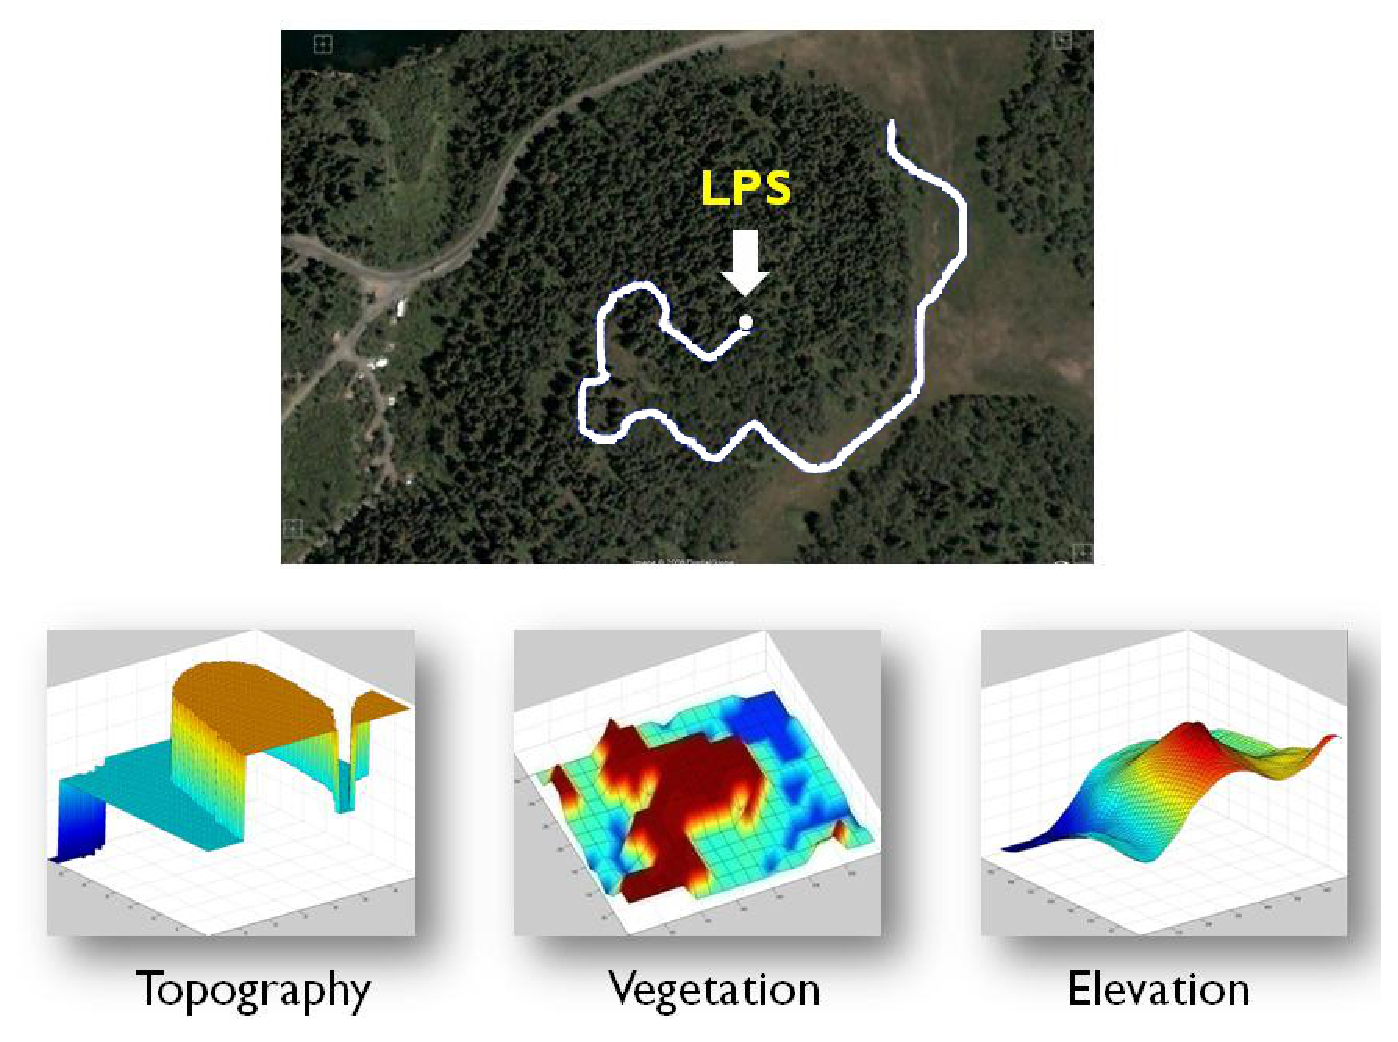
\includegraphics[width=5in]{satellite.eps}
\caption[Satellite imagery and terrain data of area by Payson Lake, Utah]{Satellite imagery of area by Payson Lake, Utah together with relative topography, vegetation, and elevation data downloaded from USGS web site. The topography and vegetation plots are discretized into (lake, plain, hill), and (sparse, medium, dense) respectively.}
\label{satellite}
\end{figure}

%---------------------------------------------------
\subsection{Hexagonal Tessellation Discretization}
\label{sec:3.3}

The first step in the model is to discretize the area into a hexagonal tessellation as shown in Figure~\ref{hexgrid}. The reason we use a hex tessellation is because the hex tessellation ensures the distance from the center of one cell to the center of any neighboring cell is always the same. The width of each hex cell is 24 meters. We picked this number because we believe such a granularity allows us to have enough detailed information about the terrain features without going into excessive details to burden the amount of computation. Future work should systematically explore how changing this granularity affects the tradeoffs between computational complexity and precision. In a real WiSAR scenario, the width can also be determined by the level of detail available for the terrain feature data at hand.

\begin{figure}
\centering
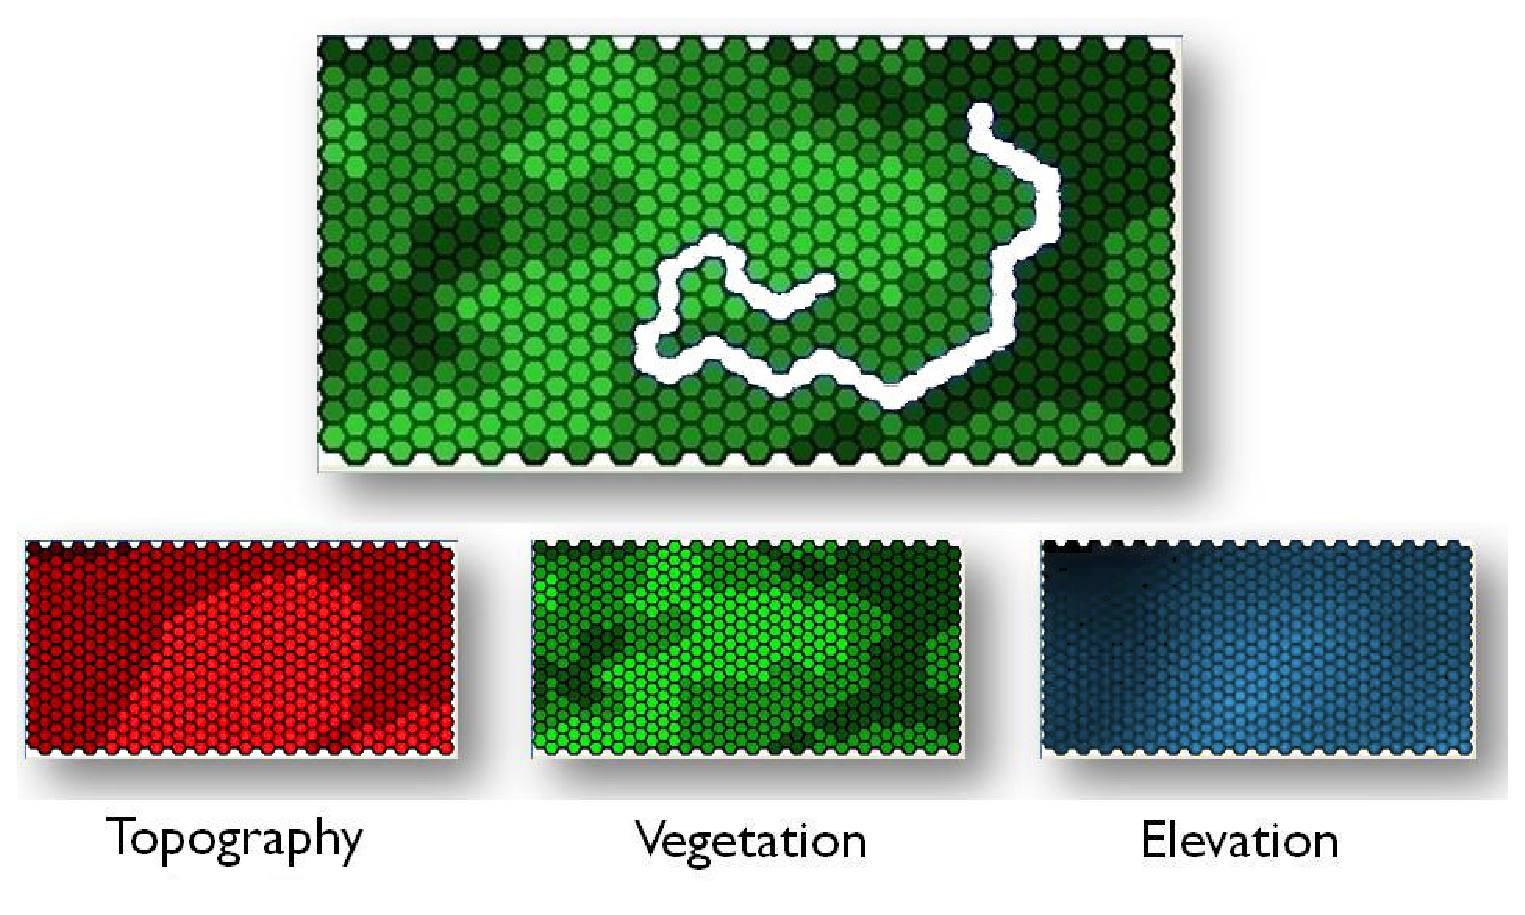
\includegraphics[width=5.5in]{hexgrid.eps}
\caption[Hexagonal discretized tessellation showing past historical data]{Hexagonal discretized tessellation showing past historical data (the path marked by the white cells in the main image) together with topography, vegetation, and elevation information in hexagonal tessellation.}
\label{hexgrid}
\end{figure}

The resulting tessellation is a $16 \times 38$ tessellation with 608 distinct states. Using the terrain feature data we have, each state is really a 3-tuple of (topography type, vegetation type, elevation). When we transition from one state to another neighboring state (including remaining in the same state), we can identify whether the topography type and vegetation type change. By calculating the elevation difference between the two states, we can find out whether the local slope is going uphill, downhill, or neither. Here we decide whether there is a local slope by calculating the angle of the elevation difference. If the difference is more than 20 degrees, we mark it as a local slope. We subjectively picked the threshold of 20 because we want to emphasize the extra effort of going uphill (as might be representative of a typical missing person such as a 14-year-old scout). Future work should systematically evaluate the impact of this threshold on usefulness of the probability distribution function.

%---------------------------------------------------
\subsection{Model Representation}
\label{sec:3.4}

In this sub-section, we define the Bayesian model in terms of the prior, the state transition, and the likelihood, and discuss each component in detail.

%*****************************
\subsubsection{The Prior}
\label{sec:3.4.1}

With the knowledge of past WiSAR incidents and expert opinion on human behavior, we can ask domain experts to specify their prior beliefs on how the missing person would behave with respect to different terrain features (e.g., a transition from a medium vegetation type to a dense vegetation type). For example, since we have three different topography types, we need a $3 \times 3$ transition matrix as shown in Equation~(\ref{matrix}), representing the probability of transitioning from one topography type to another. The rows and columns are both indexed by the different topography types, and it is possible to remain in the same topography, yielding
\begin{equation}
\left[
\begin{array}{ccc}
T_{00}' & T_{01}' & T_{02}'\\
T_{10}' & T_{11}' & T_{12}'\\
T_{20}' & T_{21}' & T_{22}'\\
\end{array}
\right]
\label{matrix}
\end{equation}
For example, $T_{00}'$ is the transitional probability for remaining in the lake type topography, and $T_{00}'$ is a number between 0 and 1 inclusive. The definition of the transition matrix requires that the values in each row of the matrix sum up to 1.

However, we would also like to enable the domain experts to incorporate uncertainty in their beliefs. Therefore, for each topography transition, instead of a number, a continuous Beta distribution is used, and a probability value, such as $T_{00}'$, can be generated by sampling from the Beta distribution. We use a Beta distribution because the domain of a Beta distribution's probability density function is $x \in [0; 1]$, which matches the parameter space of probability values. The curves of the Beta distribution also have the shape we desire because the mean and the mode of the curve can shift between 0 and 1 with various variances depending on what parameters we pick (illustrated in Figure~\ref{BetaPDF}). To specify uncertainty, for each topography transition probability, we ask the domain experts to provide a mean and a variance because these parameters are much easier to understand for non-statisticians compared to the $\alpha$ and $\beta$ parameters for the Beta distribution. Then we solve for the $\alpha$ and $\beta$ parameters automatically.

\begin{figure}
\centering
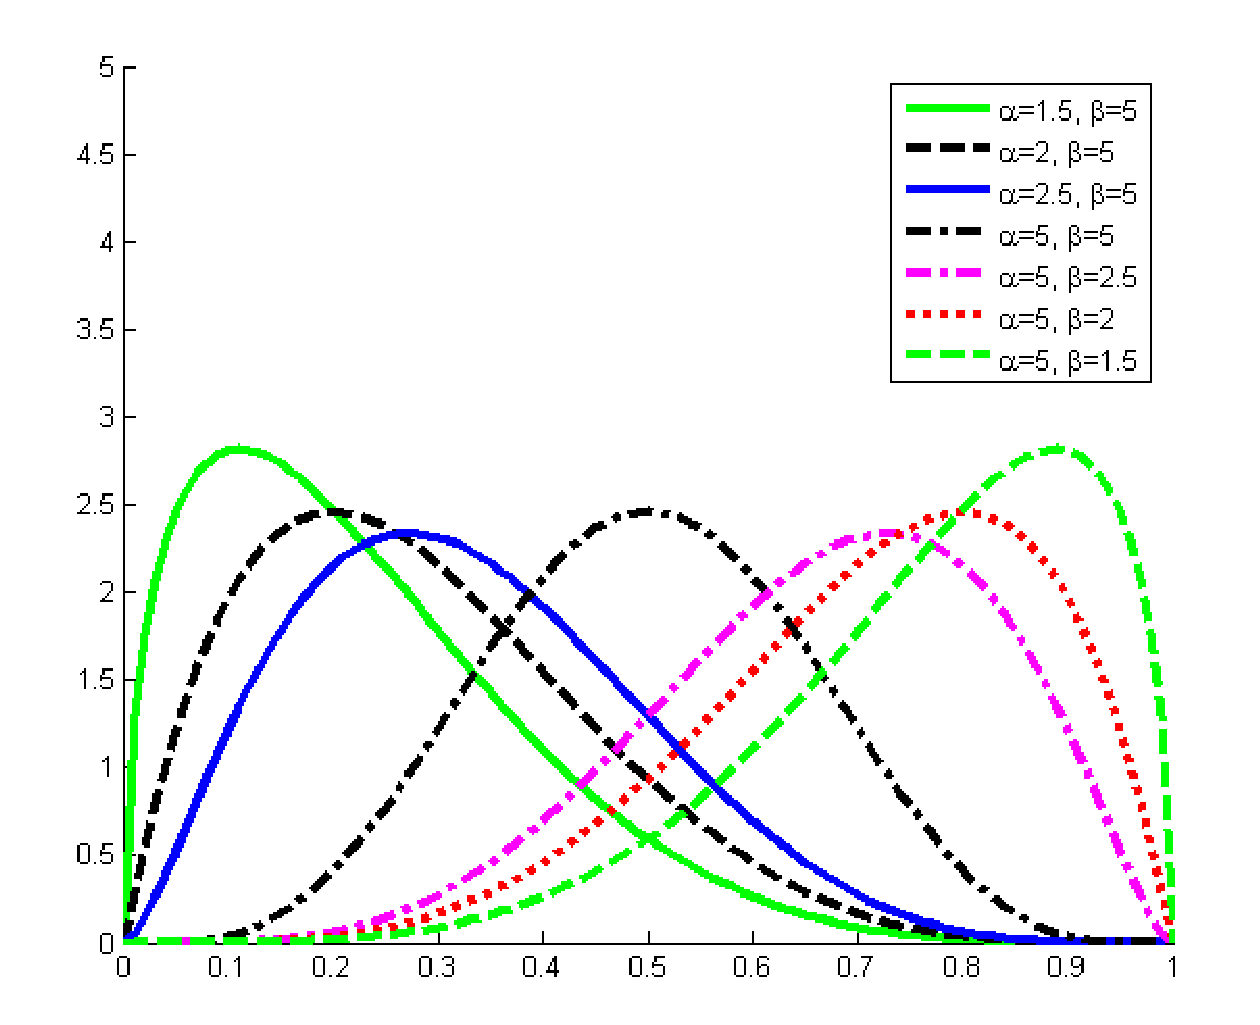
\includegraphics[width=5in]{BetaPDF.eps}
\caption[Beta Distribution probability density function]{Beta Distribution probability density function}
\label{BetaPDF}
\end{figure}

We have to be careful here to make sure the transition matrix, shown in Equation~(\ref{matrix}), is still valid. For example, the domain experts can specify means for Beta distributions relating to transitioning from topography type ``plain'' to all three topography types as 0.5, 0.3, and 0.2. These numbers sum up to 1. Unfortunately when we sample from the three Beta distributions, the values we get could possibly be something like 0.5, 0.35, and 0.22, which do not sum up to 1. That means these numbers are not true probability values, and we have to normalize them so they become true probability values. Therefore, we use $T_{ij}$ to denote the value we generate from the Beta distribution corresponding to transitioning from topography feature $i$ to topography feature $j$, and use $T_{ij}'$ to denote the true probability value (after normalization) for the transition. The probability distributions of $T_{ij}$ are the domain experts' prior beliefs with respect to topography terrain features, and there are 9 of them.

Similarly, since we have three different vegetation density types, we also need a $3 \times 3$ transition matrix to represent the probability of transitioning from one vegetation density type to another. This adds 9 vegetation density related priors to the model. With respect to local slopes, since there are only three possible transitions (uphill, no slope, and downhill), there are only 3 more priors to specify.

Therefore, our model has a total of 21 priors (9 related to topography, 9 related to vegetation density, and 3 related to local slope). For simplicity, we denote the joint distribution of all the priors as $\pi(\underline{\theta})$, where 
\begin{align}
\label{21}
\underline{\theta} &=T_{00},T_{01},...,T_{22},V_{00},V_{01},...,V_{22},S_0,S_1,S_2
\end{align}
and each prior follows a Beta distribution with known $\alpha$ and $\beta$ values (solved using the mean and variance values provided by domain experts). Thus
\begin{align}
\label{BetaT}
T_{ij} \sim Beta(\alpha_{T_{ij}}, \beta_{T_{ij}})\\
\label{BetaV}
V_{ij} \sim Beta(\alpha_{V_{ij}}, \beta_{V_{ij}})\\
\label{BetaS}
S_{i} \sim Beta(\alpha_{S_{i}}, \beta_{S_{i}})
\end{align}
where $T_{ij}$ represents the probability of transitioning from topography type $i$ to $j$ (possibly $i=j$) where $i=0,1,2$ and $j=0,1,2$. Similarly, $V_{ij}$ represents the probability of transitioning from vegetation type $i$ to $j$, and $S_{i}$ represents the probability of following a certain local slope type $i$.

%*****************************
\subsubsection{State Transition}
\label{sec:3.4.2}

In an earlier part of the paper we described how the search area is discretized into a hexagonal tessellation. Each cell becomes a state. Let $X$ represent a state, then $X$ can be defined as a vector containing information about the hexagonal cell:\\

\indent{}$X$ = [topography, vegetation density, elevation, index of tessellation]\\

With our model, we assume the state transition follows a first-order Markov process, meaning that the next state the lost-person (LP) will be in is only dependent on the current state the LP is in.
\begin{align}
\label{FirstOrder}
P(X_t|X_0, X_1, ..., X_{t-1}) = P(X_t|X_{t-1})
\end{align}

This is a strong assumption and it might not hold. For example, the amount of time traveled following the same direction (e.g., 20 minutes) could affect whether the LP wants to turn around and backtrack; similarly, the intended destination might affect which path the LP chooses while looking for the way. However, we argue that because the LP is in a disoriented state (although the LP might think otherwise) in the wilderness, the direction the LP follows could very well not be the direction the LP thinks he/she is following. Therefore, this assumption should not prevent the model from having useful predictive power. However, we also plan to extend the model in future work that will take into consideration the intended destination and incorporate that information into the representation of the current state.

When we compute $P(X_t|X_{t-1})$, it is necessary to combine the topography transition probability with vegetation density and local slope so we can borrow strength from each of the terrain features. We denote $T(Y|X)$ as the probability of transitioning from the topography of state $X$ to the topography of state $Y$, and $V(Y|X)$ as the probability of transitioning from the vegetation density type of state $X$ to the vegetation density type of state $Y$. Using the elevation difference between state $X$ and state $Y$, we can identify the local slope of going from state $X$ to state $Y$. We denote $S(Y|X)$ as the probability of transitioning from state $X$ to state $Y$ only based on local slope information. $T(X|Y)$, $V(X|Y)$, and $S(X|Y)$ are all true probability values, and they correspond to the relevant entries in the terrain features transition matrices such as Equation~(\ref{matrix}). Assuming the three terrain features are independent of each other we can combine the three probabilities by taking the product of the three,
\begin{align}
\label{product}
P(X_t|X_{t-1}) \propto T(X_t|X_{t-1})V(X_t|X_{t-1})S(X_t|X_{t-1}),
\end{align}
where $P(X_t|X_{t-1})$ is the entry in the row indexed by $X_t$ and the column indexed by $X_{t-1}$ in the state transition matrix describing the probability of transitioning from any state to any other state (including transitioning into the same state). Here $P(X_t|X_{t-1})$ is a true probability value.

Because a person can only travel from one hexagonal cell to its neighboring cells (or remain in the original cell), in each row of the state transition matrix, the transitional probabilities for all $X_t \notin N(X_{t-1})$ will be 0, where $N(X_{t-1})$ is the set of neighboring states of state $X_{t-1}$ (including $X_{t-1}$). That means the sum of $P(X_t|X_{t-1})$ for all $X_t \in N(X_{t-1})$ is 1 (elements in each row of the state transition matrix should sum to 1). 

If we look at each hex cell closely, we can see that from each cell a person can travel to one of the six neighboring cells or remain in the same cell. 
\begin{align}
\label{sub}
\mathrm{Let}~\underline{\phi'} &= P(X_t|X_{t-1}) ~\mathrm{where}~ X_t \in N(X_{t-1})\\
\mathrm{Let}~\underline{\phi} &= T(X_t|X_{t-1})V(X_t|X_{t-1})S(X_t|X_{t-1}) ~\mathrm{where}~ X_t \in N(X_{t-1})
\end{align}

We know $\underline{\phi}$ and $\underline{\phi'}$ each have 7 elements, and $\sum_{i=1}^7 \phi_i' = 1$, where
\begin{align}
\label{phi}
\phi_i' = \dfrac{\phi_i}{\sum_{j=1}^7 \phi_j}
\end{align}

Equation~(\ref{phi}) normalizes the products of terrain feature transition probabilities to compute the $P(X_t|X_{t-1})$ entries for all neighbors of state $X_{t-1}$.

%*****************************
\subsubsection{The Likelihood}
\label{sec:3.4.3}

Because from each cell a person can travel to one of the six neighboring cells or remain in the same cell, the likelihood of one observation (how the lost person traveled from one cell to one of the neighboring cells), denoted as $f(z|\underline{\theta})$, follows a categorical distribution with 7 dimensions. Relating to the previous section, $z$ can be defined as
\begin{align}
z = (X_t, X_{t-1}), ~\mathrm{where}~ X_t \in N(X_{t-1}).
\end{align}
In other words, $z$ is really a vector in the form of a 7-tuple, but to avoid notation confusion, we will only use $\underline{z}$ to denote multiple observations in a later section when we discuss posteriors. If we use $z_i$ to represent each element in vector $z$, then $z_i$ is constrained by
\begin{align}
\label{}
z_i \in \{0,1\} ~\mathrm{and}~ \sum_{i=1}^7 z_i=1,
\end{align}
meaning exactly one element in the 7-tuple is 1 and the others are all 0s. For example, an observation can be of the form of (0,0,0,0,1,0,0), meaning the person traveled to the fifth neighboring cell. Thus, our observation given all the prior beliefs is governed by
\begin{align}
\label{CAT}
z|\underline{\theta} &\sim CAT(\underline{\phi'}), ~\mathrm{where}\\
\underline{\phi'} &= \phi_1', \phi_2', ..., \phi_7', ~\mathrm{and}\\
%\end{align}
%\begin{align}
\label{likelihood}
f(z|\underline{\theta}) &= \prod_{i=1}^7 \phi_i'^{z_i},~\mathrm{where}\\
\underline{\theta} &= T_{00},T_{01},...,T_{22},V_{00},V_{01},...,V_{22},S_0,S_1,S_2.
\end{align}

Note that in order to compute the likelihood for $z$ using Equation~(\ref{likelihood}), we need to identify $X_{t-1}$, the state the person is in, and all neighboring states $X_t \in N(X_{t-1})$. We also need to sample from our priors $\pi(\underline{\theta})$ in order to construct terrain features transition matrices, which are then used in Equations~(\ref{sub}) --~(\ref{phi}) to compute $\underline{\phi'}$.

Figure~\ref{BN} illustrates the process of computing the likelihood graphically. The top row shows the 21 priors we sample from to generate $\underline{\theta}$ (9 for topography, 9 for vegetation density, and 3 for local slope). After normalization, we obtain all the entries for the terrain features transition matrices as shown in the second row (9 priors from the $3 \times 3$ topography transition matrix: $T_{00}', T_{01}', ..., T_{22}'$, 9 from the $3 \times 3$ vegetation density transition matrix: $V_{00}', V_{01}', ..., V_{22}'$, and 3 local slope probabilities: $S_0, S_1, S_2$). Depending on the $X_{t-1}$ and $X_{t}$ states associated with $z$, relevant $T(X_t|X_{t-1})$, $V(X_t|X_{t-1})$, and $S(X_t|X_{t-1})$ probability values are identified and multiplied to compute $\underline{\phi}$ (third row). The elements of the $\underline{\phi}$ vector are further normalized to produce $\underline{\phi'}$ (fourth row), which are the probabilities of the lost person traveling from state $X_{t-1}$ to all the neighboring states.

\begin{figure}
\centering
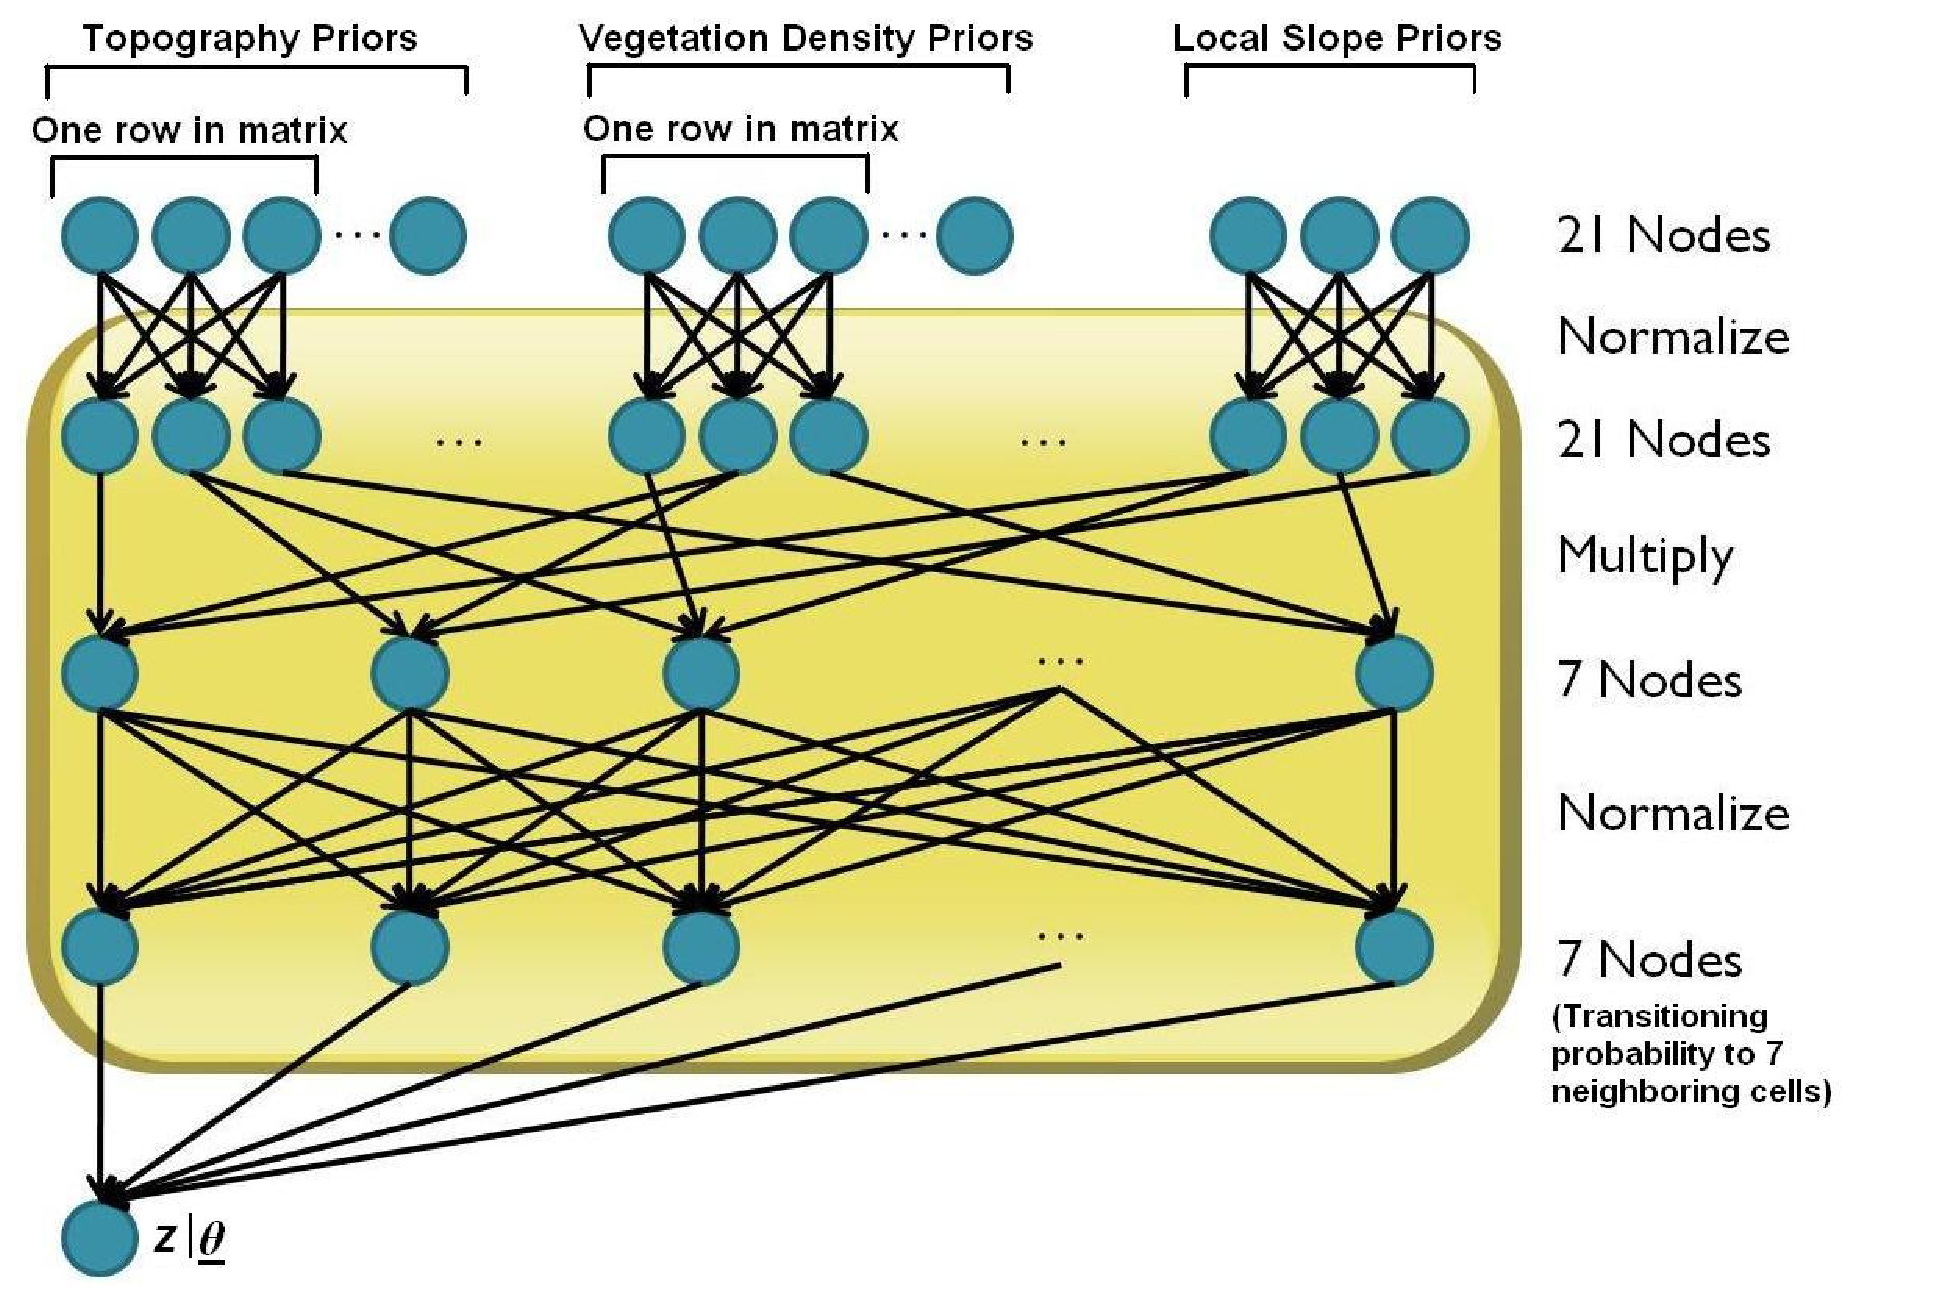
\includegraphics[width=6in]{BN.eps}
\caption{A graphical illustration of the proposed model. Top row: probability distribution for each prior belief. Fourth row: probability of transitioning into a neighboring cell in the hex tessellation. Bottom row: an observation indicating possible travel directions for the lost person.}
\label{BN}
\end{figure}

Once samples are generated from the priors $\pi(\underline{\theta})$, we can deterministically compute the values for the middle layers --- they are simply delta functions. Therefore, when we build the Bayesian network to compute the posteriors, we collapse all the middle layers and only keep the top and bottom layers.

%---------------------------------------------------
\subsection{Using the Model to Compute the Posterior}
\label{sec:3.5}

A great benefit of using a Bayesian model is that we can incorporate existing observations to update prior beliefs. The updated beliefs are the posterior beliefs.

Existing observations in the model are in the form of sections of GPS track logs (also discretized to a hexagonal tessellation) together with the terrain features associated with the track logs. By combining existing human behavior data with prior beliefs, we can reduce the domain experts' uncertainty.

To incorporate multiple observations, we simply add multiple $z|\underline{\theta}$ nodes in the bottom row of the Bayesian network (illustrated in Figure~\ref{BNPost}). The network is dynamically built with appropriate parent nodes identified and linked to the observation nodes dynamically.
\begin{figure}
\centering
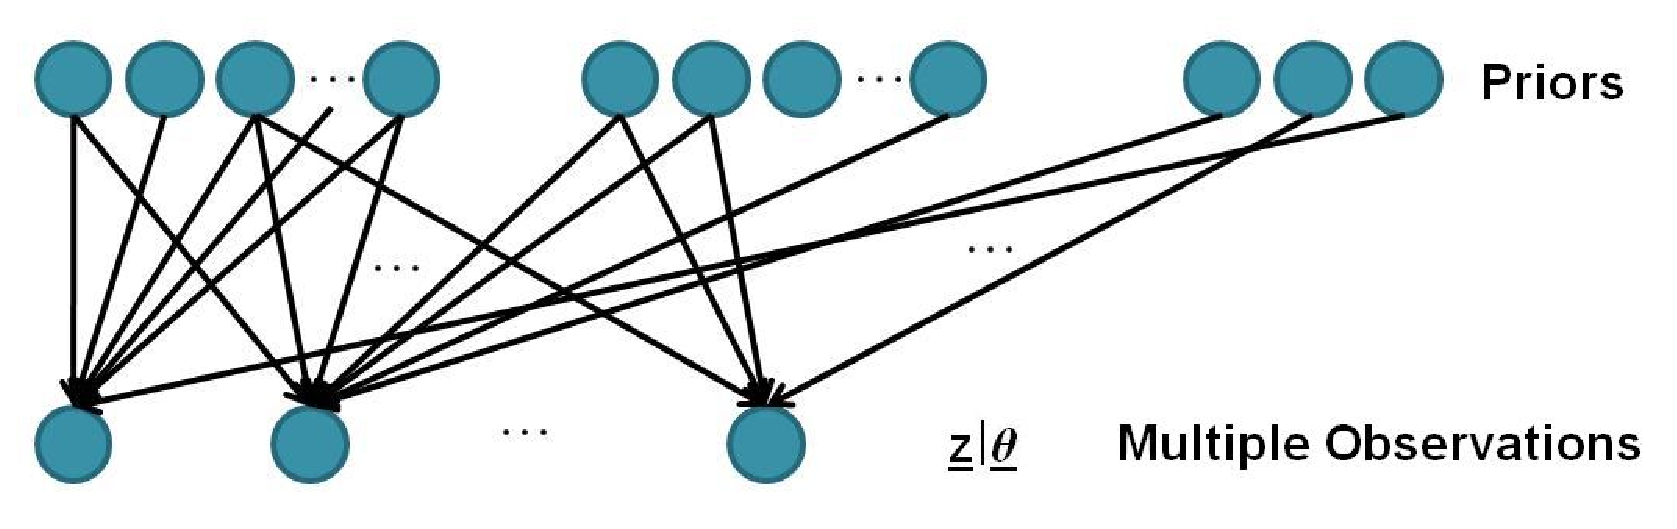
\includegraphics[width=6in]{BNPost.eps}
\caption{Bayesian network with multiple observations. Top row: probability distribution for each prior belief. Bottom row: multiple observations from previously collected human behavior data in the form of segments of GPS track logs together with terrain features associated with the track logs.}
\label{BNPost}
\end{figure}

Because of the complexity of the model, it is impossible to solve for the posterior distribution $\pi(\underline{\theta}|\underline{z})$ in closed form. That is why we used an MCMC approximation algorithm as the generation tool. Specifically, we used a random walk flavor of MCMC that uses the Gibbs Sampling algorithm, shown in~\cite{Gelman2004Bayesian}, on the outside loop, with Metropolis-Hastings algorithm, shown in~\cite{Gelman2004Bayesian}, inside each iteration of the Gibbs Sampling. Gibbs sampling is an algorithm for generating samples from a joint probability distribution of multiple random variables when the conditional distribution of each variable is known. It generates samples from the distribution of each variable in turn, conditioned on the current values of other variables. The Metropolis-Hastings algorithm generates a first-order Markov chain in each state and uses a proposal density, which depends on the current state, to generate a new proposed sample. This value is accepted if a value drawn from a uniform distribution between 0 and 1 meets certain requirements. Otherwise, the current value is retained. In our implementation, we used a Gaussian function as the proposal density.

In our implementation, we used 500 iterations for burn (throwaways) and kept 10,000 samples for each parent node. In each iteration, the Gibbs Sampling algorithm tries to sample from the distribution of each parent node in turn, conditioned on the current values of other parent nodes. However, Gibbs Sampling relies on the Metropolis-Hastings algorithm to really generate samples from the posterior distribution by using a proposal density function (a Gaussian distribution in our case). These samples approximate the posterior distribution for each of our 21 priors. 

Figure~\ref{Approximation} illustrates how the Monte Carlo method approximates the posterior distribution of one parameter (a parent node). In each iteration, the Metropolis-Hastings algorithm probabilistically generates a sample for the node based on the complete conditional constructed by Gibbs sampling (points inside smaller graphs in the upper portion where each point represents a probability value generated from a Beta distribution). If we combine all these samples into one graph and bin the points into small clusters (bigger graph in lower portion where the y axis is the count), we can connect the top of the bins and draw a curve. This curve is an approximation of the posterior distribution of the node, and as the number of samples approaches infinity, the curve matches the actual posterior distribution.

\begin{figure}
\centering
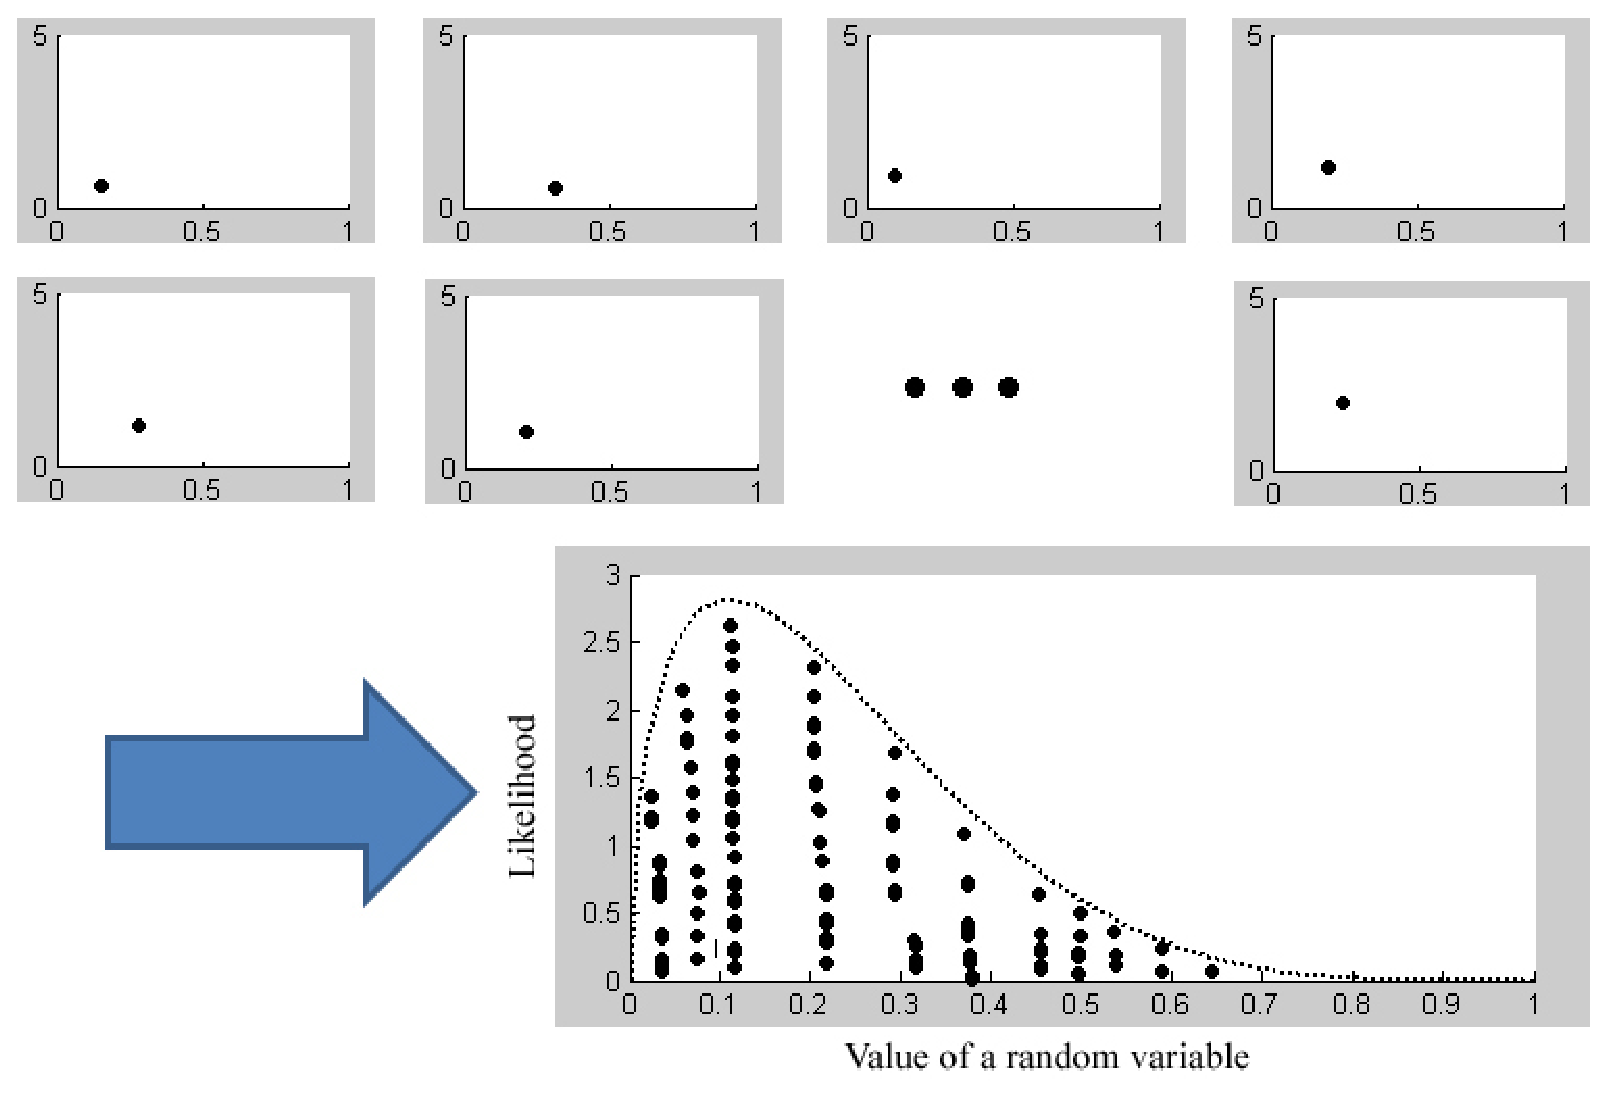
\includegraphics[width=5.5in]{Approximation.eps}
\caption{Graphical illustration of how the Monte Carlo method approximates the posterior distribution of one parameter. Upper: multiple iterations of sampling. Lower: samples clustered to approximate the real distribution.}
\label{Approximation}
\end{figure}

In our experiments, the MCMC algorithm completed in 220~seconds on a Dual-core AMD 3800+ PC with 3GB of memory.

%---------------------------------------------------
\subsection{Using the Model to Compute the Predictive Probability Distribution}
\label{sec:3.6}

Using the model described above, once we have the priors specified, we can build our $608 \times 608$ state transition matrix. In our implementation, we sample once from each Beta distribution for each time step. Starting from the lost person's point last seen, we can generate the prior predictive probability distribution by multiplying the state transition matrix in each time interval. This method allows the search and rescuers to see how the predictive probability distribution changes as time progresses.

~\cite{Setnicka1980Wilderness} and~\cite{Syrotuck2000Introduction} show that in WiSAR scenarios, as time progresses, the effective search radius increases by approximately 3km/hour, which is equivalent to 50m/minute. Because the age of the lost-person affects the speed the person travels, we can adjust the size of the time interval accordingly. With our lost scout scenario, because children generally travel slower than adults, we assume the lost scout travels at roughly 24m/minute; therefore, we define each time step as 1 minute. When we multiply the state transition matrix (sampled once from the prior distributions at each time step) 200 times (3 hours and 20 minutes = 200 minutes), we have the prior predictive probability distribution map as shown in the upper row of Figure~\ref{priorvspost}.

Once we combine previously collected human behavior data and approximate the joint posterior distribution of all the parameters, we can sample from the posterior beliefs instead of the prior beliefs. Following the same state transition matrix multiplication, we can also generate the posterior predictive probability distribution. The lower row of Figure~\ref{priorvspost} shows this distribution. In the Wilderness Search and Rescue case, the posterior predictive probability distribution is the 2D probability distribution map we are seeking.

\begin{figure}
\centering
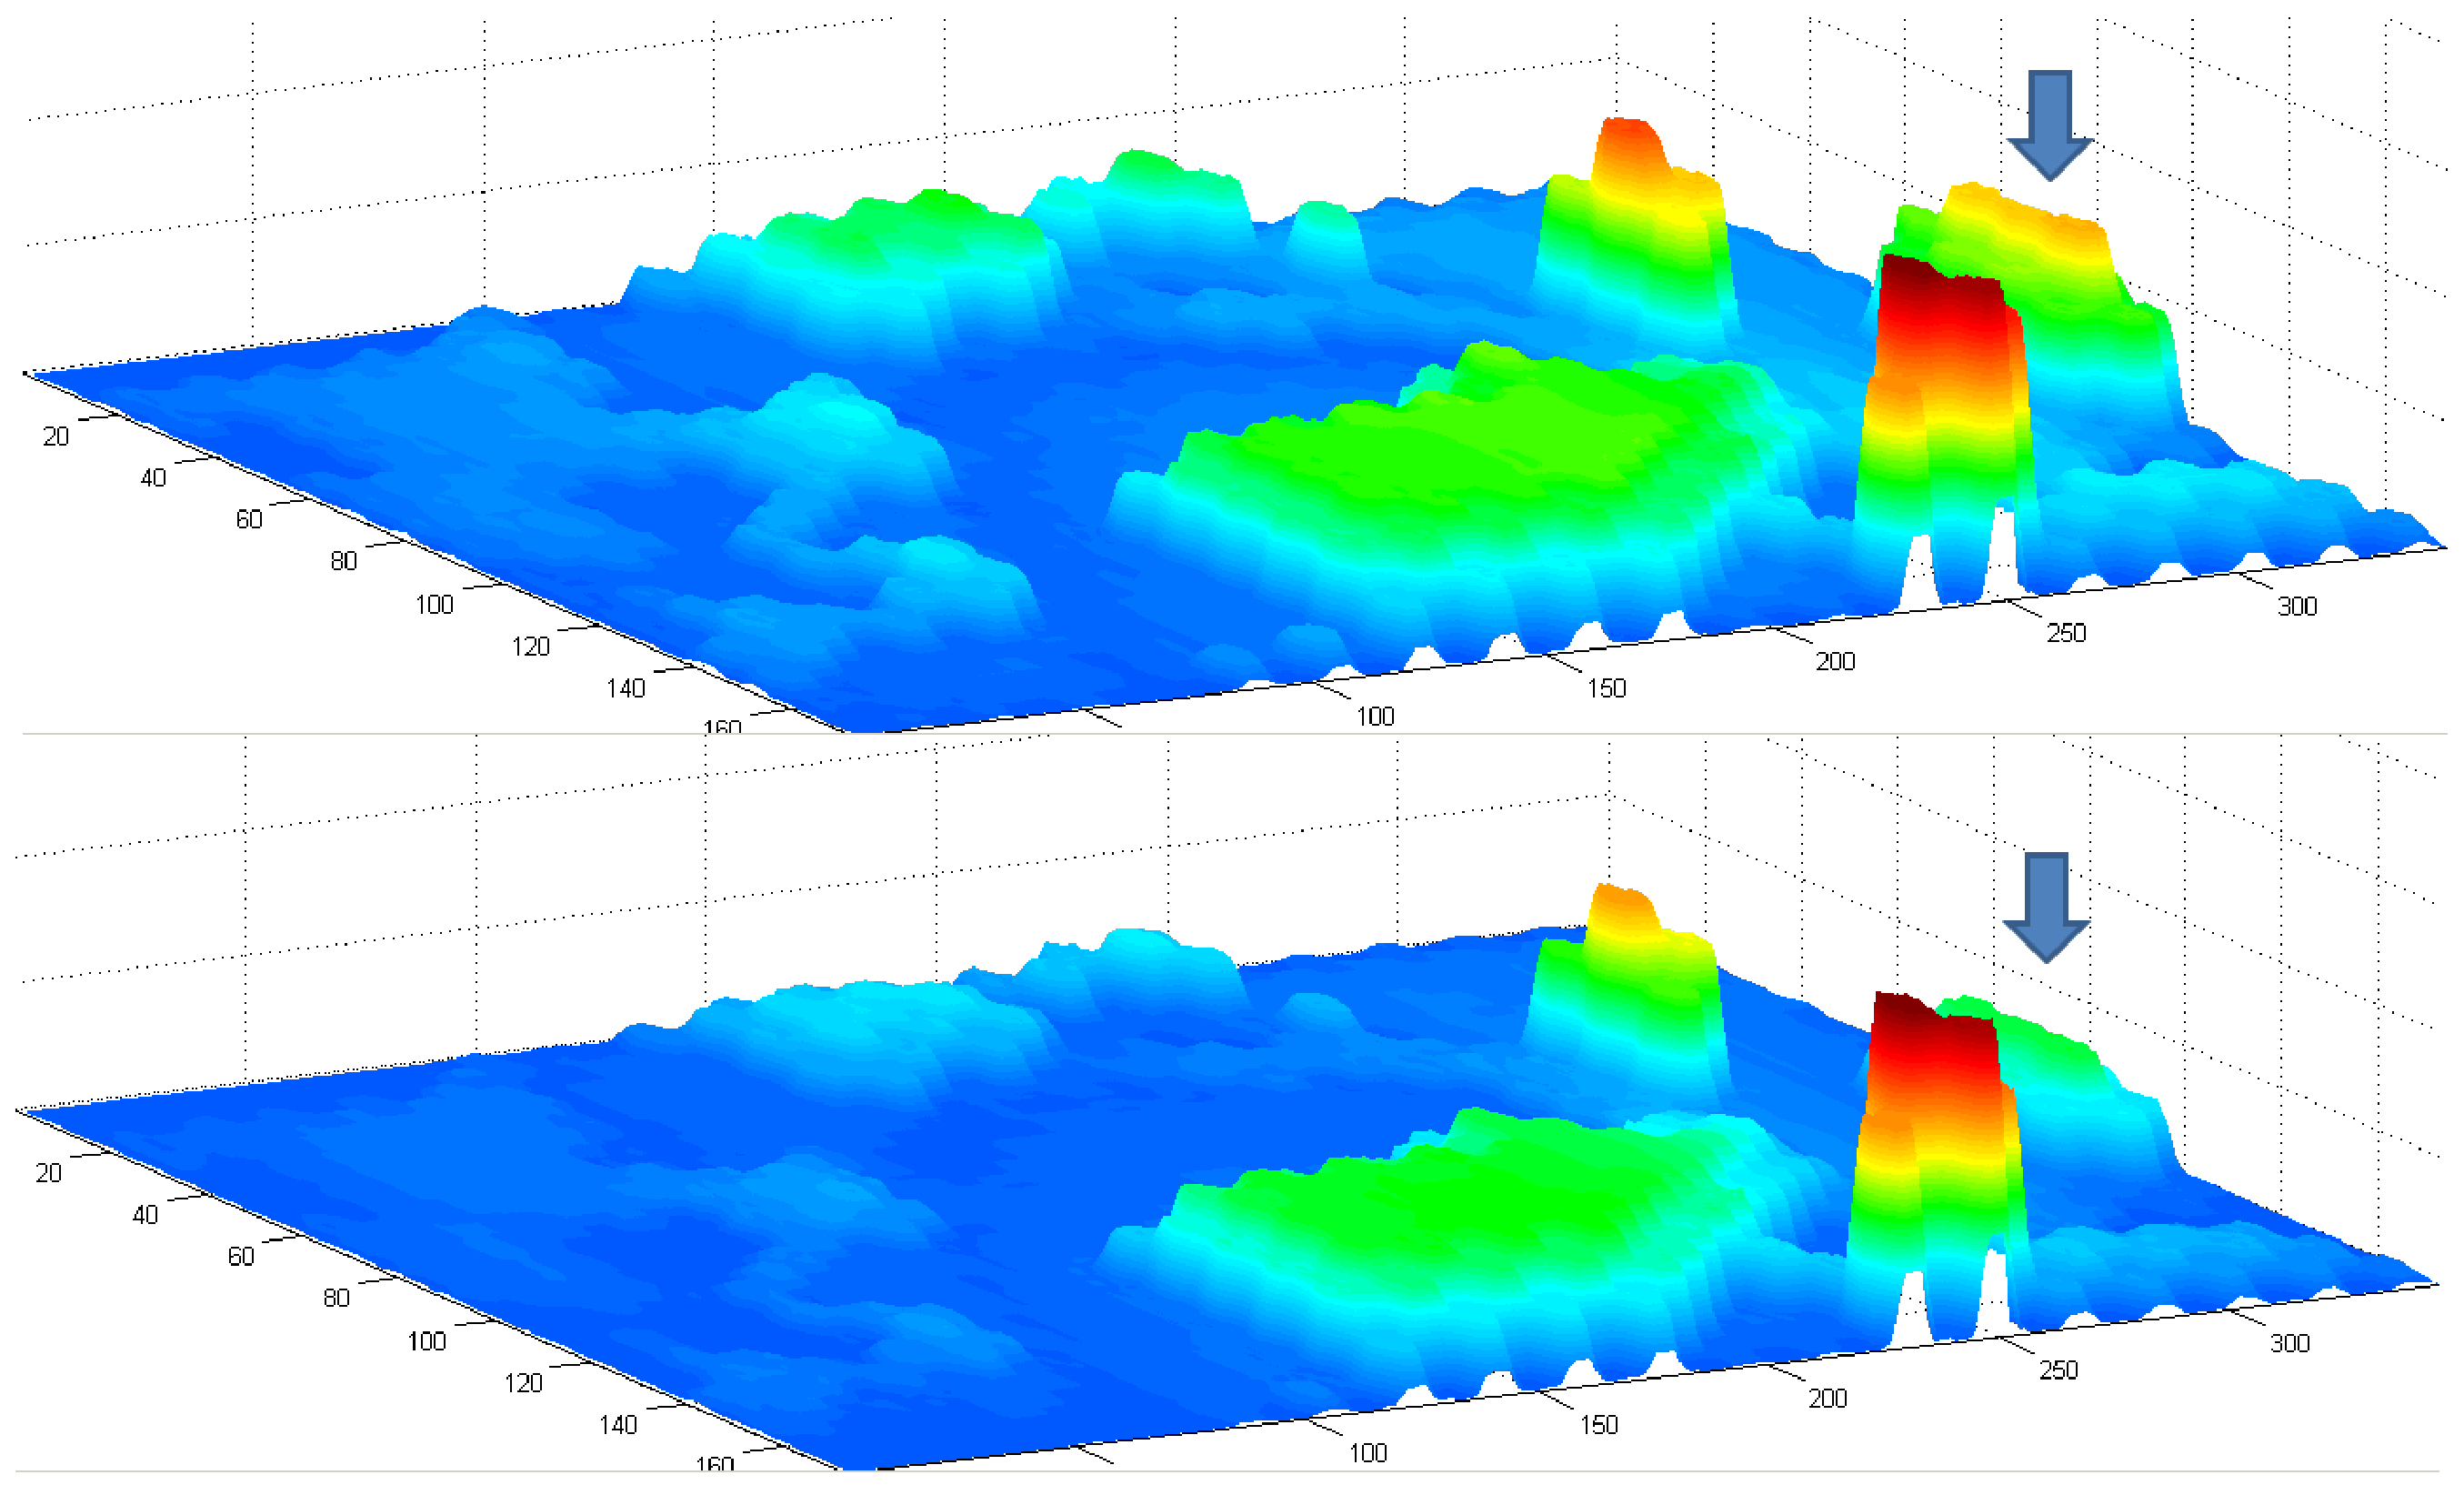
\includegraphics[width=6in]{priorvspost.eps}
\caption[Comparing prior predictive distribution against posterior predictive distribution]{Comparing prior predictive distribution (upper row) against posterior predictive distribution (lower row)}
\label{priorvspost}
\end{figure}

%=====================================================================================================
\section{Evaluation of the Model}
\label{sec:4}

%---------------------------------------------------
\subsection{Synthetic Data}
\label{sec:4.1}

Pretending to be domain experts, we specified all the prior distributions by setting the means and the variances. The matrices below show the prior distributions we set for the vegetation type transition matrix. The first matrix shows the means and the second matrix shows the variances.
\begin{equation}
\centering
\left[
\begin{array}{ccc}
\mu_{V_{00}}=0.6 & \mu_{V_{01}}=0.25 & \mu_{V_{02}}=0.15  \\
\mu_{V_{10}}=0.5 & \mu_{V_{11}}=0.3 & \mu_{V_{12}}=0.2  \\
\mu_{V_{20}}=0.4 & \mu_{V_{21}}=0.4 & \mu_{V_{22}}=0.2  \\
\end{array}
\right]
\end{equation}
\begin{equation}
\centering
\left[
\begin{array}{ccc}
\sigma^2_{V_{00}}=0.14^2 & \sigma^2_{V_{01}}=0.15^2 & \sigma^2_{V_{02}}=0.1^2 \\
\sigma^2_{V_{10}}=0.15^2 & \sigma^2_{V_{11}}=0.15^2 & \sigma^2_{V_{12}}=0.15^2 \\
\sigma^2_{V_{20}}=0.15^2 & \sigma^2_{V_{21}}=0.15^2 & \sigma^2_{V_{22}}=0.15^2 \\
\end{array}
\right]
\end{equation}

We set these values following common sense. For example, we believe a lost scout is more likely to remain in sparse vegetation type ($\mu_{V_{00}}=0.6$) and unlikely to transition from a sparse vegetation type to a dense vegetation type ($\mu_{V_{02}}=0.15$). We also believe a lost scout is more likely to transition from a dense vegetation type to a medium or sparse vegetation type and from a medium vegetation type to a sparse vegetation type ($\mu_{V_{21}}=0.4$, $\mu_{V_{20}}=0.4$, $\mu_{V_{10}}=0.5$). However, for most of these Beta distributions, we are not certain about our estimation, which is why we specified large variances for most of the parameters. For example, $\sigma^2_{V_{10}}=0.15^2$ means we believe the probability to transition from vegetation type medium to sparse could be as low as 0.05 and as high as 0.95. In real WiSAR scenarios, the priors should come from past statistical analysis of lost-person behaviors, such as~\cite{Heth1998Characteristics} and~\cite{Syrotuck2000Analysis}, combined with domain experts' opinions.

Each observed data point is a transition from one cell to another neighboring cell (including remaining in the same cell) in previously collected GPS track logs. The track logs do not even have to be in the same search area of the current incident. What we really care about is how terrain features affect a person's behavior in the wilderness. If the track logs contain this kind of information, we can use it to update our prior beliefs. These posterior beliefs can then be used in a generative approach to predict how the lost person might travel from the point last seen as time progresses. For the lost scout scenario, our observed data is partly shown in Figure~\ref{hexgrid} as the path of white cells. We use the word ``partly'' because during the travel, the person sometimes stayed in the same state during the 1-minute time interval. To test the robustness of the model, we intentionally designed the data set so that the person remained in the same vegetation type most of the time. We also repeated the same path three times in our synthetic dataset to simulate three different past GPS track logs. By repeating these we are basically adding more strength to the data and we expect the data to have a much stronger effect on the posterior distributions for the parameters. Each path consists of 45 transitions; therefore, our dataset has 135 data points.



%We are currently in the process of collecting real human behavior data in the form of GPS track logs from hikers\footnote{http://alltrails.com/}, hunters, and geocachers\footnote{http://tanglefoot.cs.byu.edu/~amy/index.html}. Note that historical datasets from different areas can be used together to generate posterior distributions for the same set of parameters, but samples generated from the posterior distributions will be used on the same search area in order to generate predictive distributions.

%---------------------------------------------------
\subsection{Prior vs. Marginal Posterior}
\label{sec:4.2}

Using the posterior samples, we can compare the marginal prior distribution with the marginal posterior distribution for each of our parameters. Figure~\ref{posts} shows the comparison for some of the parameters. The dotted lines represent the prior distributions and the solid lines represent the posterior distributions.

The plot in the upper left is for parameter $T_{02}$, the terrain feature transition probability from lake to hill. Since we do not have any data point in our dataset that transitioned from lake to hill, here we see the posterior is almost identical to the prior. The plot in the upper right is for parameter $T_{12}$, the terrain feature transition probability from plain to hill. In our dataset, a good segment of the path basically followed the contour line but stayed in the plain states. This characteristic of the dataset explains why the posterior distribution is much narrower and had a much lower mean---because the data did not show many changes from plain to hills, the posterior probability of this transition is much lower with less variance. The plot in the lower left is for parameter $V_{01}$, the terrain feature transition probability from vegetation type sparse to medium. The plot in the lower right is for parameter $S_1$, the terrain feature transition probability from no slope to no slope. Both of these posteriors are only slightly different from the priors.
\begin{figure}
\centering
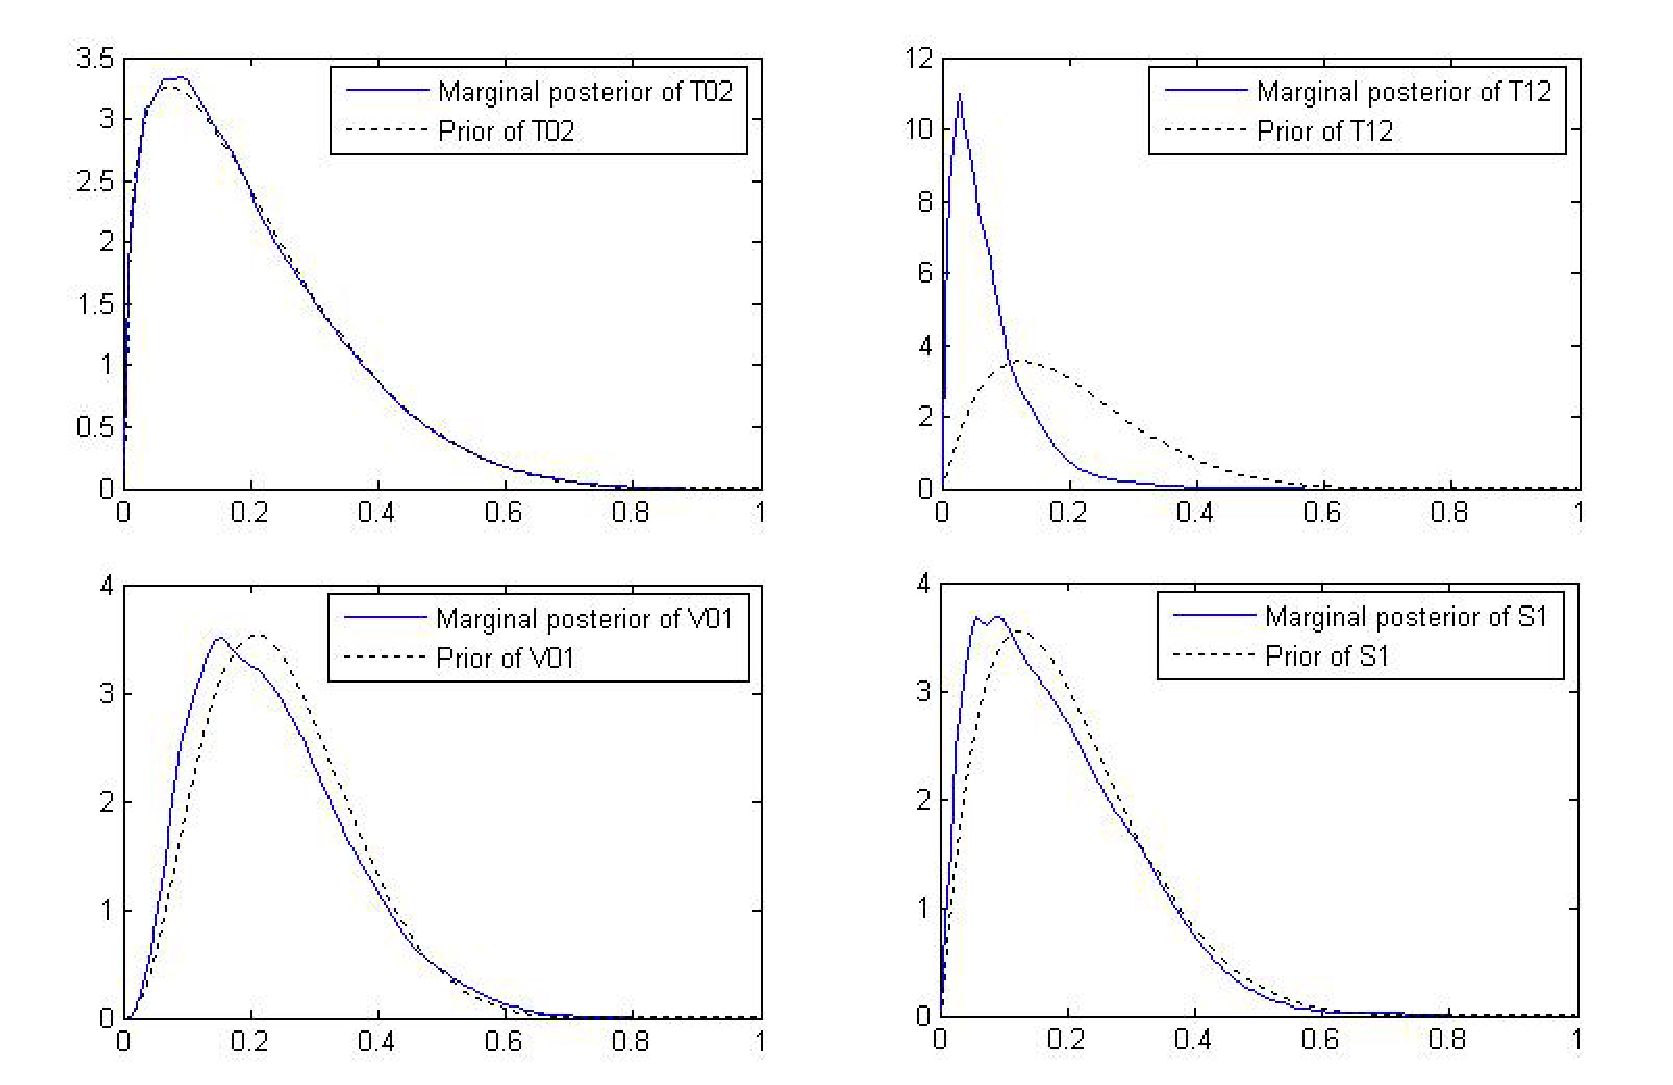
\includegraphics[width=6in]{posts.eps}
\caption[Comparing prior distribution with marginal posterior distribution]{Comparing prior distribution with marginal posterior distribution. Upper Left: $T_{02}$ Upper Right: $T_{12}$ Lower Left: $V_{01}$ Lower Right: $S_1$.}
\label{posts}
\end{figure}

%---------------------------------------------------
\subsection{Correlation of Parameters}
\label{sec:4.3}

When we ask the domain experts to specify the priors, we assume the parameters are independent. Because we have 21 parameters, the joint posterior distribution in the parameter space is really a distribution with 21 dimensions, which is impossible to plot. Instead, we use a correlation image to show whether there exist correlations between pairs of parameters.

Figure~\ref{correlation} shows a graphical representation of the correlation between each pair of parameters. A grey value, such as cell(1,21) in the lower left corner, indicates that there is no correlation between the two parameters. A white cell, such as cell(1,1) in the upper left corner, means the two parameters are fully positively correlated, and a black cell means the two parameters are fully negatively correlated. Here we see that the vegetation parameters $V_{20}$ (dense to sparse), $V_{21}$ (dense to medium), and $V_{22}$ (dense to dense) showed positive correlation. Other positive correlations also mostly appear between neighboring parameters. There is also a clear positive correlation between $V_{22}$ (Vegetation: dense to dense) and $S_{0}$ (uphill). These positive correlations are marked by the big circle in Figure~\ref{correlation}.

The results of the correlation analysis indicate that there is likely a correlation among different terrain features. Interestingly, from this figure we can see that parameter $V_{12}$ (Vegetation: medium to dense) and $T_{11}$ (Topography: plain to plain) are clearly, negatively correlated (marked by the upper small circle in Figure~\ref{correlation}). Parameter $V_{22}$ (Vegetation: dense to dense) and $T_{11}$ (Topography: plain to plain) are also clearly, negatively correlated (marked by the lower small circle in Figure~\ref{correlation}). A closer look at the terrain features of the area shows that dense vegetation is mostly located on the hill topography type and medium vegetation is mostly located on the plain topography type. This explains why we see such a negative correlation. This emergence of correlations that are compatible with terrain features suggests that the process of combining prior information with observed track logs is useful. However, when we let the domain experts specify the prior distributions, it is much more intuitive for them to assume independence instead of specifying conditional probabilities (to specify how the parameters are correlated), and we rely on data to identify the dependence relationship.
\begin{figure}
\centering
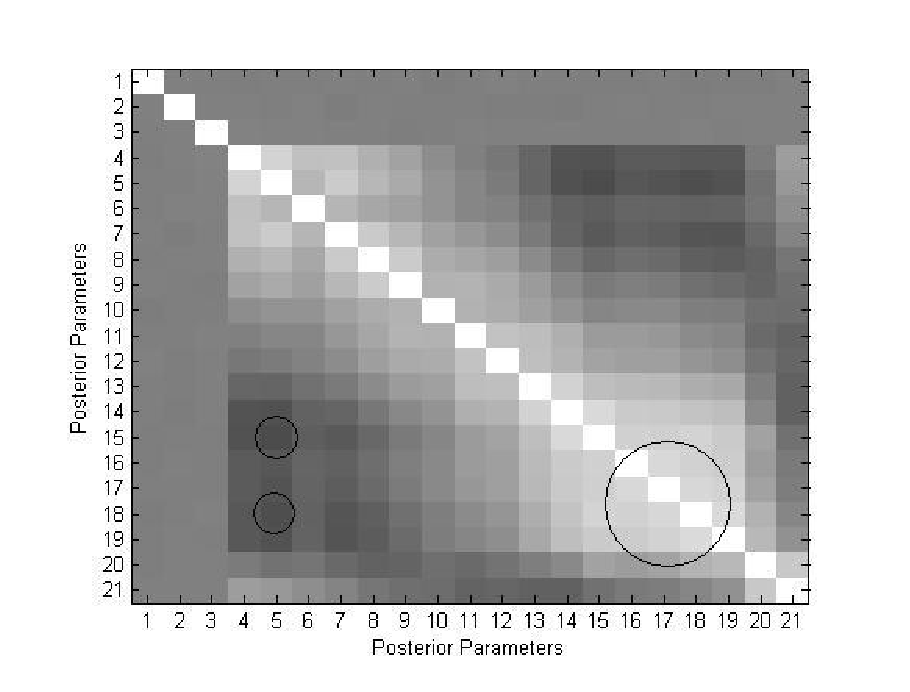
\includegraphics[width=6in]{correlation.eps}
\caption[Parameter correlation]{Parameter correlation: a grey value of 128, such as (1,21) in the lower left corner, represents no correlation. A white cell, such as (1,1) in the upper left corner, represents a correlation of 1. A black cell represents a correlation of -1. Parameters are in the following order: $T_{00},T_{01},...,T_{22},V_{00},V_{01},...V_{22},S_{0},S_{1},S_{2}.$ The big circle marks a positive correlation between parameters, and the small circles mark a negative correlation between parameters.}
\label{correlation}
\end{figure}

%---------------------------------------------------
\subsection{Prior Predictive vs. Posterior Predictive}
\label{sec:4.4}

In this section we compare the prior predictive probability distribution and the posterior predictive probability distribution. The prior predictive is generated by sampling from the prior beliefs specified in the first part of the model. The posterior predictive is generated by sampling (using MCMC) from the posterior beliefs generated from the first part of the model. If no previous human behavior data is available, then the prior predictive can still be used to show likely places to find the missing person; otherwise, the posterior predictive should be used because combining existing human behavior data enables the model to reduce uncertainty in the posterior beliefs.

Both probability distributions use a generative approach to predict how the lost person might travel from the point last seen as time progresses. The 2D probability distribution map generated is the final product of the model and can be used by Incident Commanders in WiSAR operations.

The lower row of Figure~\ref{priorvspost} shows the posterior predictive distribution created using the samples generated for all the parameters through MCMC. After 200 time steps (equivalent to 3 hours and 20 minutes), we can see that near the right side of the map, clearly much less probability mass is allocated compared with the prior predictive distribution (indicated by arrows). The center of the northern region also has lower probability compared with the prior predictive distribution, but the difference is not dramatic. Therefore, with our lost scout scenario, this posterior predictive probability distribution map suggests that we should send search and rescue workers to the regions marked by the two highest peaks first to maximize the likelihood of finding the missing scout.

%=====================================================================================================
\subsection{Bayesian \texorpdfstring{$\chi^2$}{Chi-squared} Test for Goodness-of-Fit}
\label{sec:4.5}

We used the Bayesian $\chi^2$ test for goodness-of-fit proposed by~\cite{Johnson2004Bayesian} to evaluate the  quality of posterior beliefs in the proposed model. This test is closely related to the classical $\chi^2$ goodness-of-fit statistic, but different in many aspects. The classical $\chi^2$ goodness-of-fit test computes a single $p$-value. The Bayesian version, however, computes the goodness-of-fit at each iteration of the MCMC, conditional on the current set of model parameter values sampled from the posterior distribution of all the model parameters. The posterior distribution of the resulting $p$-values converges to a $\chi^2$ distribution with $k-1$ degrees of freedom as the number of iterations approaches infinity. \cite{Johnson2004Bayesian} defined the Bayesian $\chi^2$ test for goodness-of-fit using the following equation:
\begin{align}
R^B(\vec{\tilde{\theta}}) = \sum_{k=1}^K {\left [\dfrac{(m_k(\vec{\tilde{\theta}})-n p_k)}{\sqrt{n p_k}}\right ]}^2
\end{align}
where $\vec{\tilde{\theta}}$ is a set of model parameters sampled from the posterior distribution in a single iteration, $m_k(\vec{\tilde{\theta}})$ represents the number of observations that fell into the $k$th bin, $n$ is the total number of observations, and $p_k$ is the probability assigned by the null model to this interval. Values of $p_k$ are held fixed while the bin counts $m_k(\vec{\tilde{\theta}})$ are considered as random quantities.

Because our likelihood function is a categorical distribution with 7 parameters (a discrete distribution) we used 7 bins, so $k=7$. It is worth mentioning that $p_k$ is different for each data point in our case. For each set of model parameters, we calculate the probability values (for each neighbor of the cell, into which the data point fell) for the 7 bins for each observed data point, and then sum up all the probability values for each bin across all data points. By dividing the sum for all bins, we normalize the probability value, and the result is the probability for that bin.

With $k-1=6$ degrees of freedom, we computed the $\chi^2$ distribution and then computed the quantiles (the $p$-values) for each of the 10,000 $R^B(\vec{\tilde{\theta}})$ values. The results show that only 6 out of 10,000 $p$-values are smaller than 0.05, the statistical significance value we selected. The Bayesian $\chi^2$ test of goodness-of-fit suggests that our model fits the synthetic dataset well.

%=====================================================================================================
\section{Discussions and Limitations}
\label{sec:5}

First we summarize some of the assumptions made throughout the development of the model and our rationale behind them. We assume that the state transition follows a first-order Markov process. Our argument is that the lost person is likely in a disoriented state, therefore, the assumption should not be a big problem (see section~\ref{sec:3.4.2} for more details). Another assumption is that the three terrain features are independent. Although correlation analysis shows possible dependence between terrain features, we believe it is more intuitive for domain experts to assume independence instead of specifying conditional probabilities, and we rely on data to identify the dependence relationship (see section~\ref{sec:4.3} for more details). We also assume that the Markov process is stationary with homogeneous time steps (see section~\ref{sec:3.6} and section~\ref{sec:4.4}). However, we argue that the flexibility of specifying finer time intervals and the possibility to stay in the same state can ``simulate'' a non-stationary process with various time durations, thus alleviating the restriction.

After analyzing 162 lost-person incidents near Peter Lougheed Provincial Park in Alberta, Canada, \cite{Heth1998Characteristics} come to the conclusion that there is a close correlation between a lost-person's intended destination and the angle of dispersion (calculated from the lost-person's point last seen and the point the person was eventually found). This finding suggests that it might be a good idea to incorporate the missing person's intended destination into our existing model.

One limitation of this paper is that we are using synthetic data for our evaluation. To address this, we recently collected all the GPS track logs within the US that were uploaded to the popular web GPS track log repository, everytrail.com. We were able to identify 329 GPS track logs that contained the word ``geocache'' (or ``geocaching''). Because most of the geocache ``treasures'' are hidden in the wilderness off of a designated trail, we believe that GPS track logs created by geocachers are likely to contain behavior data indicating how a human might react to different terrain features. After closer examination of these track logs, we see a clear trend that the locations of the geocache ``treasures'' play an important role in the person's behavior in the wilderness in addition to terrain features. If we want to use this kind of GPS track log data as existing human behavior data, our model has to take into consideration the intended destination.

Another trend we observed from these GPS track logs is that a majority of the geocachers first followed some trails to get closer to the ``hidden treasure''. When the trail starts to clearly lead the person further away from the geocache, or when the person decides to take a shortcut somewhere along the trail, the geocacher then abandons the trail and creates a new path.

During the summer of 2009, a student in our research lab went for a geocache hunt near Box Elder Peak in Utah. After successfully finding the ``hidden treasure'', he decided to not return the same way he came from, but to try some alternative route. Soon he found himself lost and struggled for several hours to reorient himself. Eventually he stumbled onto a hiking trail, a different one from what he took before completing the geocache mission, then he followed the trail and found his way back. Figure~\ref{BoxElderPeak} shows the GPS track log displayed in Google Earth for the period when he was off-trail and lost in the wilderness. The point we want to make here is that after running into another unknown hiking trail, he immediately decided to stay on the trail. This kind of behavior can only be predicted by models that handle trail-following, and our present model clearly lacks this capability.

We plan to extend our model to support intended destination and trail-following. Doing so would allow us to take advantage of abundant GPS track logs and incorporate such human behavior data into the posterior distribution. Once we have the newer model, we can also take advantage of the existing Bayes factor analysis methods, such as Akaike Information Criterion (AIC) proposed by~\cite{Akaike1974AIC}, Bayesian Information Criterion (BIC) presented in~\cite{Schwarz1978BIC}, and Deviance Information Criterion (DIC) described in~\cite{Spiegelhalter2002DIC}, to perform extended validation.

In the present model, for every time step, only one sample is generated from each Beta distribution. A possible improvement is to use the idea of particles. At each time step, the model would generate, for instance, 100 examples from each Beta distribution, and then compute 100 sets of categorical distributions (each has 7 discrete values representing probabilities of transitioning to 7 directions), which can then be averaged to produce a final categorical distribution with better quality and a better representation of the experts' uncertainty. Because the added computation is outside of the MCMC algorithm and the matrix multiplications, the added execution time should be minimal.

Another important question we should ask is: How well would an experienced IC trust the probability distribution map generated using the proposed model? We strongly believe that the predictive probability distribution generated using the proposed model should only be used as a base onto which domain expertise can be further projected. The objective of the model is to provide a tool that reduces the IC's workload and supports the IC's operation, but not to replace the IC's responsibilities. With abundant experience, training, and the ability to incorporate much richer information (e.g., lost person profile, weather), the IC is responsible for validating the probability distribution suggested by the model and also for coming up with the final distribution map. To really make the tool useful for ICs in WiSAR operations, two additional elements are necessary: 1) a human factors analysis (user study) of the users' trust of the algorithms and automation in the WiSAR domain, and 2) an interface component/tool that enables the IC to easily modify the probability distribution generated by the model. The ability for the IC to modify the probability distribution both at the beginning and during the search can potentially improve how (much) users trust the system and make the proposed model more acceptable to users. Future work should develop an interface tool that enables a user to modify a probability distribution map. We believe results from such research can help improve the usability and usefulness of the proposed model.

\begin{figure}
\centering
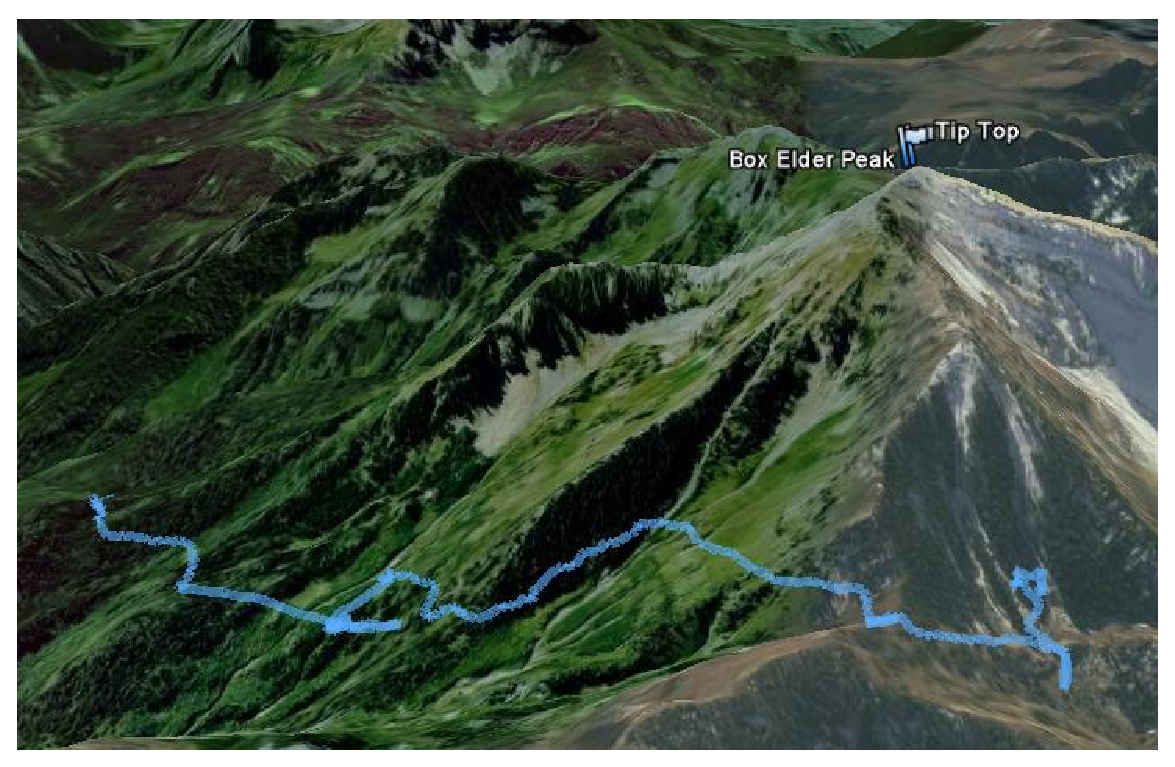
\includegraphics[width=5.5in]{BoxElderPeak.eps}
\caption[Satellite imagery of Elder Box Peak in Utah]{Satellite imagery of Elder Box Peak in Utah. The GPS track log shows the path taken by a hiker in summer 2009 when he went off the hiking trail and became lost for several hours before stumbling into another hiking trail.}
\label{BoxElderPeak}
\end{figure}



%=====================================================================================================
\section{Conclusions and Future Work}
\label{sec:6}

In WiSAR operations, the Incident Commander typically has limited resources and relies on a probability distribution map to allocate resources, to direct the search, and to coordinate rescue workers. Because as time progresses, the survivability of the missing person decreases and the effective search radius increases by approximately 3km/hour, it is critical to find the missing person quickly. That is why areas with high probabilities are searched first, and the quality of the probability distribution map can have a great impact on the search and rescue operations. We proposed a Bayesian approach to help generate such a probability distribution map by modeling lost-person behaviors based on three terrain features: topography, vegetation, and local slope. Our objectives are to ease the generation of probability distribution maps for the search and rescuers and to improve the quality of these maps.

Our proposed model uses publicly available geographic information and enables domain experts to specify uncertainty in their prior beliefs of how the missing person will transition from one terrain feature to another. Using the Bayesian model, past human behavior data in wilderness can be incorporated into the model to generate posterior beliefs. Following a first-order Markov process, the posterior beliefs can be used to build a temporal state transition matrix that allows the generation of the posterior predictive probability distribution map for any given time interval. We evaluated our model using the Bayesian $\chi^2$ test of goodness-of-fit from~\cite{Johnson2004Bayesian} because it allows the evaluation of multiple $p$-values for samples generated from the posterior parameter space. Results from the test suggest that our model fits the synthetic dataset well. The proposed Bayesian approach is promising, but we also acknowledge that the present model is limited to the proposed terrain features and could benefit from incorporating additional factors such as intended destination and trail-following.

In future experiments, we plan to let search and rescue experts specify terrain-based transitional probabilities so the prior predictive probability distribution can be generated using our model. Then we also let the experts directly specify a probability distribution on the regional map (with and without the restriction of only considering how terrain features would affect the lost-person's behavior). It would be very interesting to compare the resulting distributions and analyze the causes of any differences. However, because there is no ``ground truth'' with respect to the ``correct'' probability distribution, such comparisons will not be used as a form of validation. Instead, such information can be used to enrich prior beliefs in our model.

Future work should also explore how the generated probability distribution map can be used as a base by the search and rescue workers to reduce workload and also reduce the chance that the search and rescue workers might overlook certain areas that should have been allocated higher probabilities. It is also worth investigating what effect different spatial resolution (granularity) when sampling GPS track logs might have on the quality of the predicted probability distributions. The temporal model enables the search and rescue workers to view the dynamic changes of the probability distribution map over time. It will be beneficial to investigate further how search and rescuers can take advantage of this kind of information to improve search efficiency.

Most importantly, the proposed terrain feature-based Bayesian model is only the foundation of a larger framework. Future work should include incorporating more factors that affect lost-person behaviors into the network. Such factors include but are not limited to direction of travel, missing person profile, panicking factor, weather conditions and season of the year. The framework should allow incorporating observed data, such as a piece of clothing or candy wrapper, into the model as the search and rescue operation progresses. Our ultimate goal is to provide tools that will improve the efficiency and effectiveness of each search and rescue operation so the search and rescue workers can locate the missing persons in the minimum amount of time required, so lives can be saved.

\chapter{3D Tree Modeling Using Motion Capture}
\label{chap:treeparticles}

\noindent
Jie Long and Michael Jones. 3D Tree Modeling using Motion Capture. \emph{IEEE The Fourth International Symposium on Plant Growth Modeling, Simulation, Visualization and Application (PMA '12)}, to appear.

\begin{abstract}
Recovering tree shape from motion capture data is a first step toward efficient and accurate animation of trees in wind using motion capture data. Existing algorithms for generating models of tree branching structures for image synthesis in computer graphics are not adapted to the unique data set provided by motion capture. We present a method for tree shape reconstruction using particle flow on input data obtained from a passive optical motion capture system. Initial branch tip positions are estimated from averaged and smoothed motion capture data. Branch tips, as particles, are also generated within bounding space defined by a stack of bounding boxes or a convex hull. The particle flow, starting at branch tips within the bounding volume under forces, creates tree branches. The resulting shapes are realistic and similar to the original tree crown shape. Several tunable parameters provide control over branch shape and arrangement.
\end{abstract}

\section{Introduction}

Reconstruction of tree shape from motion capture data is an important step in replaying motion capture of trees under external forces, such as natural wind. Motion capture provides a fast and easy way to collect the locations over time of retroreflective marker locations placed on an object. In this paper, we address the problem of creating 3D tree shape from motion capture data. We also discuss best practices for collecting motion data from a tree. This research focuses on reconstructing static 3D tree shape with branching skeletons from data collected by a motion capture system.

\begin{figure*}[!t]
\centering
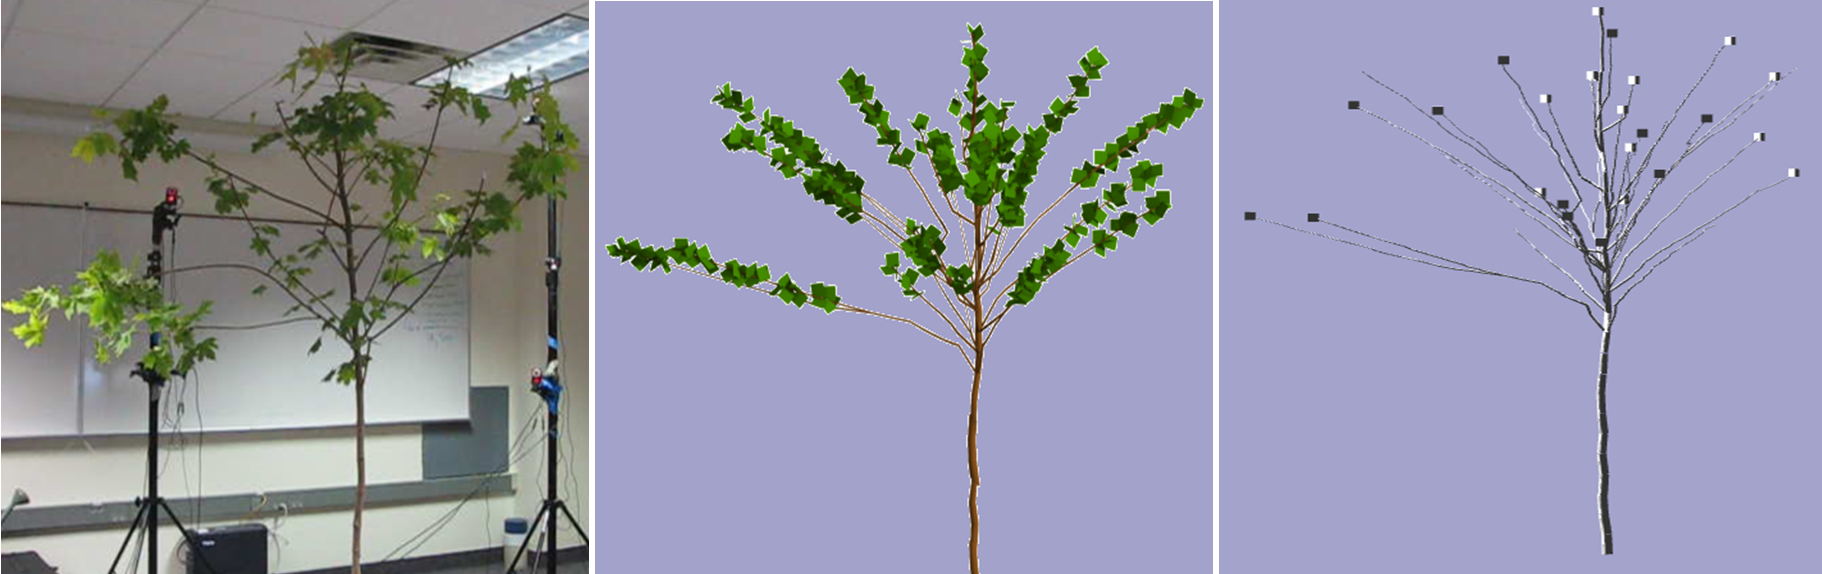
\includegraphics[scale=0.27]{Maple}
\caption{Maple model.}
\label{fig:treemodelssubfig2}
\end{figure*}

\begin{figure*}[!t]
\centering
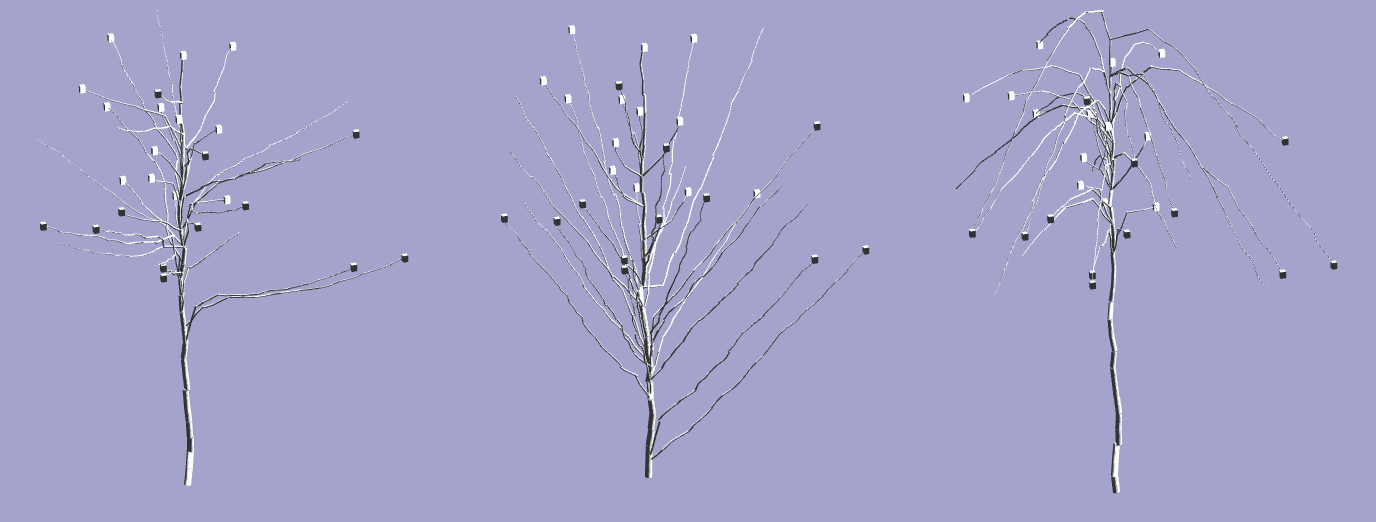
\includegraphics[scale=0.36]{varTree}
\caption{Various tree shapes generated from the same set of motion capture data. }
\label{fig:varTree}
\end{figure*}

Solutions to the motion capture problem for trees can be applied to problems in visual effects and the study of tree motion. Motion capture is a potential solution because motion capture data includes effects that are difficult to model in simulation, such as variable branch stiffness, non-uniform variation in size, and emergent effects due to leaf deformation.

Tree shape modeling has long been studied in computer graphics.  Past methods include particle systems \cite{Reeves83particlesystems,Runions07,palubicki:siggraph09,neubert:acmtg07}, L-systems \cite{lindenmayer68,Lintermann1999,Prusinkiewicz:2001}, parametric models \cite{Weber1995}, photographs \cite{RecheMartinez2004,neubert:acmtg07,Tan:2007:ITM}, and videos \cite{Li:2011:MGM,Diener:2006}. Most of these methods result in satisfying tree shapes but do not leverage the 3D positions of motion capture markers, which are recorded as part of a motion capture session but require a different set of inputs. Image- or video-based approaches convert a set of 2D input images into 3D tree models by filling in the missing dimension.  Motion capture systems can record tree shape in 3D with high precision (using similar techniques for converting a set of 2D images to a 3D model). Prior work in reconstructing tree shape from motion capture data using either exact measurements or markers placed within the crown does not scale and does not apply when leaves occlude the branching structure.

We reconstruct 3D tree shape using particle flow with motion capture data as input. Passive optical motion capture\footnote[1]{http://www.naturalpoint.com/optitrack/} records locations of reflective markers in the capture arena. We place markers only at branch tips on the edge of the tree crown. Approximately 30 markers cover the crown shape of a medium-sized tree. We do not put markers on each branch tip because passive optical motion capture systems cannot reliably track more than 70 markers. A particle flow algorithm generates branching structures starting at the recorded tip positions. Additional starting points are defined within the estimated volume of the tree crown using a vertical stack of bounding boxes or a convex hull. The bounding space approximates the tree crown and bounds particle flow and creation. The step length of a particle's flow varies with the distance to the nearest trunk point. The direction of particle motion is a combination of three forces: gravity, shape-format, and wind. The shape-format guides the particles to preserve the original tree shape. The dominant wind direction is recorded during the motion capture process. We also introduce two vectors with one pointing to the nearest trunk point and the other pointing to a constant predefined attractor point. These vectors are factors for the direction and magnitude of the forces.

In this paper, we propose a new particle flow method for reconstructing tree shape from only motion capture data. Our primary contributions are 
\begin{itemize}
	\item {a simplified particle flow algorithm for constructing tree shapes from a sparse set of branch tip positions as collected as part of motion capture and}
	\item {a method for deploying passive optical motion capture to reconstruct the shape and motion of trees in the laboratory. }
\end{itemize}

The combination of motion capture with a particle flow method provides a fast and easy approach for creating complex 3D tree shapes. The resulting tree shapes are similar to the original trees, as shown in Figure \ref{fig:treemodelssubfig2}, and can be used to replay motion similar to the captured motion. With the flexibilities of tuning the forces, we can produce several tree shapes besides the original shape. Figure \ref{fig:varTree} shows various tree shapes generated from the same set of motion capture data and demonstrates the flexibility of our forces for guiding particle flow.

\section{Related Work}

Our work is most closely related to prior work in tree modeling and applied motion capture. Our purpose is to investigate methods for creating tree shapes on which motion capture data can be replayed. Compared to prior work in modeling trees, we use motion capture as our equipment to collect partial information of tree shape and run particle flow to complete the modeling. Compared to prior work in motion capture, we design a new data collection process for non-rigid bodies and reconstruct realistic 3D models out of the data.

\subsection{Tree Modeling}

L-systems \cite{lindenmayer68} generate a tree's branching structure using axioms and rules in a concurrent context-free rewriting system. L-systems have been extended in many ways. The extension most relevant to our work is \cite{Prusinkiewicz:2001}, in which L-systems are enriched with partial differential equations and can be parameterized to reconstruct the shape of a specific tree or plant.  We chose not to investigate L-systems, or Weber and Penn's parametric tree model \cite{Weber1995}, for this application because particle flow from recorded branch tip positions closely matches the data collected in motion capture.  

More recent work in tree shape modeling involves particle systems. With the exception of Palubicki's work \cite{palubicki:siggraph09}, particle systems approximate tree shapes obtained from photographs \cite{RecheMartinez2004,neubert:acmtg07,Tan:2007:ITM}. Palubicki et al . devised a particle flow which approximates bud fate models. These methods are not directly applicable to motion capture data because these methods use photographs or environmental conditions that are not collected during motion capture.  Photographs of the tree could be taken during motion capture (and indeed are taken during optical motion capture), but we only take marker positions as input because this simplifies data collection and processing by reusing the background removal and image alignment performed as part of marker position calculation.

\subsection{Applied Motion Capture}

Motion capture has been mainly used in rigid bodies, such as human motion. It produces positions for points on an object over time with very small measurement errors.

Motion capture systems have been widely used for human or animal motion capture \cite{Lou:EHM2010,Rajko:2007:RAK,Wen:2006:MCD}. Kirk \cite{Kirk:2005:SPE} automatically generates rigid skeletons from optical motion capture systems by preserving a constant distance for each rigid part. These algorithms assume that the distance between markers on the same bone is invariant and cannot be directly applied to non-rigid bodies, such as natural trees, because the distance between markers is not invariant as the object deforms. 

Prior work in motion capture for non-rigid bodies includes several approaches to facial motion (including \cite{Ma:FPS2008,SifakisEftychios2005}). These methods are based on domain-specific features of the facial structure or patterns. Obviously these domain-specific features do not apply to tree shape reconstruction or motion capture.

The uniform branching structure of human bodies has led to well-understood processes for deploying markers on a human. The number and placement of markers is a critical part of successful motion capture using a passive optical system. Trees have a more complex and less predictable topology and require a different approach to marker placement. Previously \cite{Long:MCN2010}, researchers attempted to directly replay the motion of a tree in wind following the exact motion paths collected for all branches by putting markers on every branch of the tree. Leaves on the tree create marker occlusion, which results in poor data. In addition, manually defining branch topology to exactly match the subject tree is labor intensive. In this paper, we design a data collection and tree modeling process to overcome these difficulties by building a similar, but not exact, copy of the branching structure from a partial collection of branch tip positions. Ongoing work focuses on replaying collected motion such that the motion looks natural on an approximate copy of the branching structure.

\section{Motion Capture of Trees}
\label{sec:Motioncapturetrees}

In this section, we describe how to collect data from trees using a motion capture system such that the data supports reconstruction of tree shape. The data is collected indoors on trees with heights less than 2.5 meters. The data collection process results in an unindexed set of marker locations over time for a small set of instrumented tree branch tips. 

We use a passive optical motion capture system (Optitrack V100 by NaturalPoint)\footnote[1 ]{http://www.naturalpoint.com/optitrack/} to collect data. The passive optical capture system strikes a balance between conflicting features. Passive optical systems can reliably track up to 70 markers, and some markers weigh only a few grams. This is ideal for working with tree crowns. Active optical and active magnetic systems use heavier markers and cannot track more than 20 markers at once. The magnetic systems have the advantage of not having visibility occlusions and being able to track position and rotation, but they are more expensive than passive optical systems and can track fewer branch tips. Magnetic system markers are heavier and may alter branch tip motion.

Collecting data from natural trees is challenging for passive optical motion capture systems because trees are non-rigid bodies and are partially self-occluding. The following method for deploying passive optical motion capture systems collects data from which tree shape and motion can be inferred. 

Twelve or more cameras are arranged in a circle around the tree with six cameras located approximately 0.8 meters above the ground and another six cameras are located 3.3 meters above the ground. For each camera, the field of view is adjusted to include the entire tree. About 30 markers are placed on branch tips throughout the crown. Markers are square retroreflective markers with a surface area of about 1 cm and adhesive backing. Markers are placed to cover branch tips on each major branch from the stem and to provide nearly uniform coverage of the crown. On these branch tips, the square-shaped markers are wrapped to cover the whole tip so these markers are visible to most of the cameras from different view angles. Uniform coverage improves both shape reconstruction and motion capturing. Placing markers such that their motion paths overlap complicates algorithms for extracting motion paths from unindexed marker positions. For a medium-sized tree, the number of branch tips exceeds the number of markers so that not every branch tip is covered by a marker. Leaves around the marker are removed to improve marker visibility so the resulting 3D tree shape preserves the shape of the original tree crown. While recording tree motion we use an electric fan to create wind around the tree because data is collected indoors. The wind direction is inferred from where the fan sits relative to the tree. Other statistic methods, such as PCA (principle component analysis) can also compute the dominant wind direction after motion data of branch tips are processed.

Photographs in Figure \ref{fig:mocap} show the arrangement of the motion capture cameras and the reflective markers as deployed on an indoor pine tree. Markers are placed at branch tips shown as white dots in the image. The right side image shows marker locations in the red box on the left side image. 

\begin{figure}[!t]
\centering
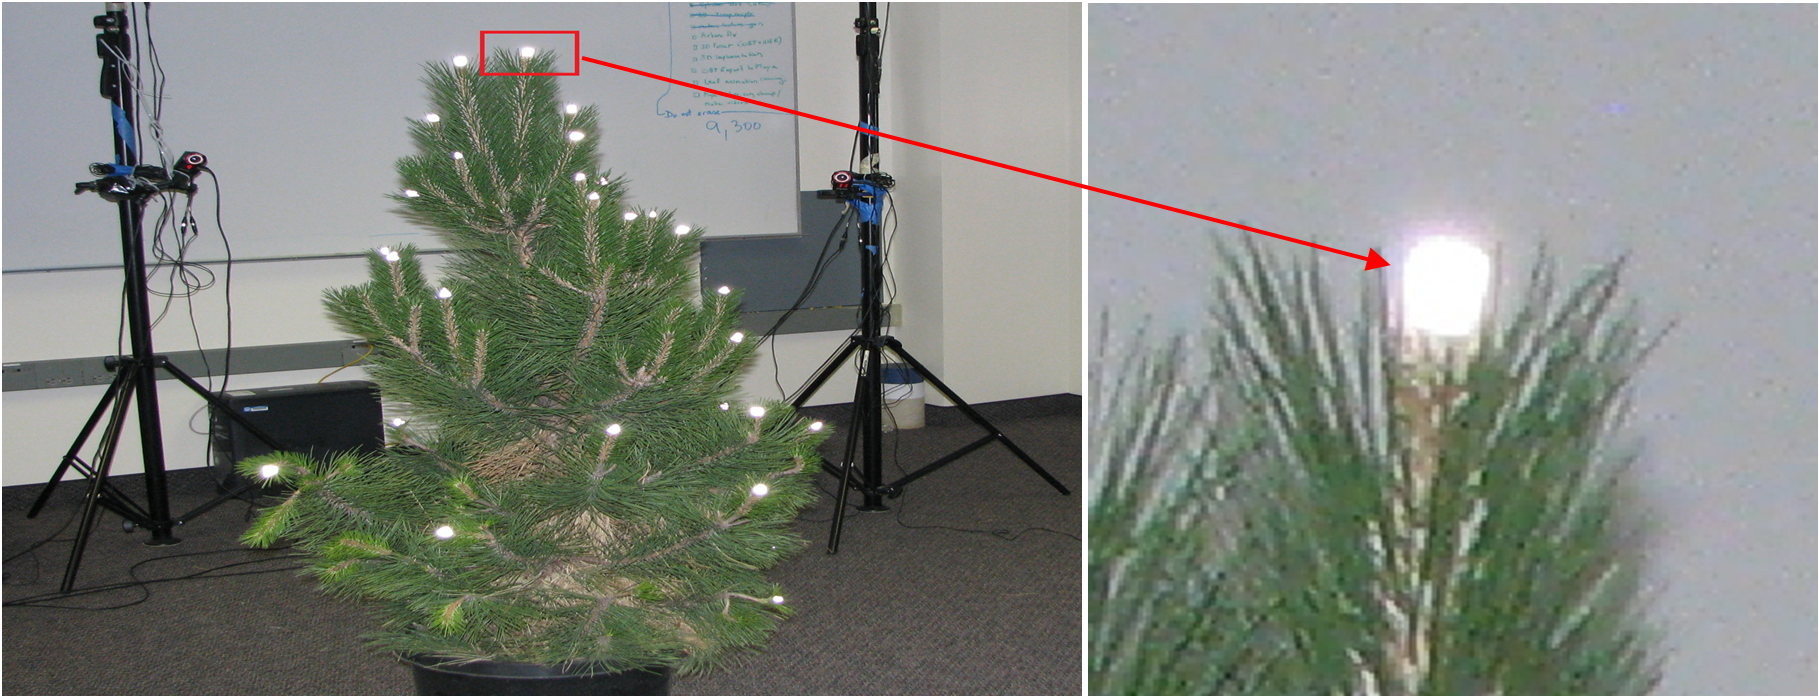
\includegraphics[width=5.0in]{Mocap}
\caption[Marker placement on the crown periphery.]{Marker placement on the crown periphery avoids occlusion while generating data that can be used to generate crown structure.}
\label{fig:mocap}
\end{figure}

Our design requires less user intervention, produces cleaner motion capture data , and may support animation of tree motion.

\section{Data Processing}
\label{sec:Dataprocessing}

Simply inferring positions from one frame of captured data is not adequate due to noise. These branch tips with markers are called "recorded" or "captured" tips. However, the initial locations of recorded branch tips may contain errors due to noise in either the system or the capture environment. 

A clustering algorithm approximates a single initial position from a collection of captured initial positions for recorded branch tips while minimizing error from the motion capture system. The clustering algorithm analyzes positions over many frames of motion capture data and eliminates gaps and noise. Gaps occur when a marker is not present in a frame. This algorithm uses forward differencing to predict a position for a marker at frame $M$ based on positions in previous frames. The closest marker in the next frame is added to the motion trace for the marker if there is a marker located close enough to the predicted position. If there is no marker position recorded close enough to the predicted position, that marker is marked with no data, i.e. a gap, for that frame. Gaps are repaired using interpolation over the motion path for a marker. If the number of marker positions recorded for a marker over time is less than $1/4$ of the total frames, that partial marker trace is marked as noise and eliminated.

If the capture process includes several hundred frames of data in which the tree is not moving, averaging branch tip positions over these frames results in precise estimates of initial positions. In most cases, the number of markers inferred from the clustering process matches the number of markers placed on the tree.

\section{Generating 3D Tree Shape}

Particle flow is a well-studied approach to generating 3D branching structure for trees \cite{Reeves83particlesystems,Runions07,palubicki:siggraph09,neubert:acmtg07}. We adapt the method to motion capture data. The 3D tree crown boundary inferred from motion capture data constrains the particle range and preserves the original 3D tree silhouette. We use a stack of bounding boxes or convex hulls to represent the crown boundary. Particles, either generated randomly in the boundary or locations of branch tips recorded by motion capture, are moving towards trunk nodes. Three forces---gravity, internal force, and external force---drive the particle flow process. The paths of the particle flow produce branching structure. By attaching leaves to the branching structure, we generate a 3D tree model that has similar appearance as the natural tree shape. 

We synthesize a trunk in the center of the crown shape, as shown in Figure \ref{fig:PineTrunk}. Figure \ref{fig:PineTrunksubfig1} shows a photograph of a pine tree with markers placed on its crown. Figure \ref{fig:PineTrunksubfig2} contains a bounding box of these marker locations and a straight vertical line representing trunk shape. The length of the line is scaled by the crown height of the bounding box. On this line segment, we generate about 10 trunk nodes. Random offsets to these nodes in the x and z direction are added as shown in Figure \ref{fig:PineTrunksubfig3}.

\begin{figure}
\centering
        \begin{subfigure}[b]{0.22\textwidth}
                \centering
                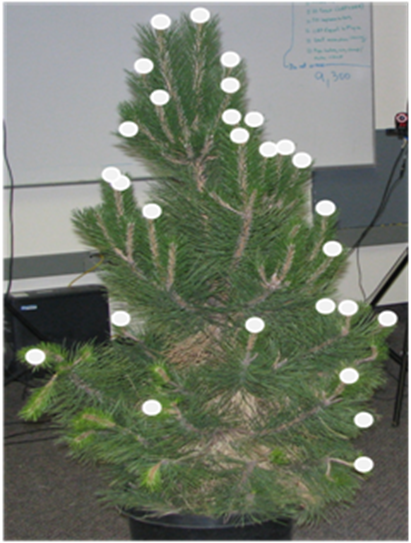
\includegraphics[width=\textwidth]{PineTrunk1}
                \caption{A pine tree with markers.}
                \label{fig:PineTrunksubfig1}
        \end{subfigure}
        ~
        \begin{subfigure}[b]{0.31\textwidth}
                \centering
                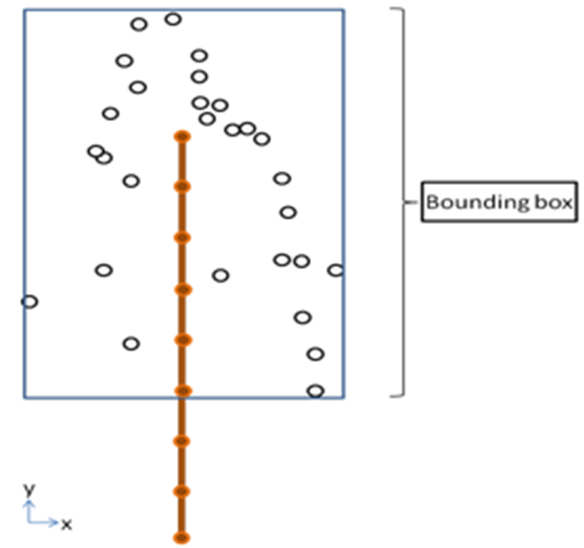
\includegraphics[width=\textwidth]{PineTrunk2}
                \caption{A straight line represents the trunk.}
                \label{fig:PineTrunksubfig2}
        \end{subfigure} 
        ~
        \begin{subfigure}[b]{0.30\textwidth}
                \centering
                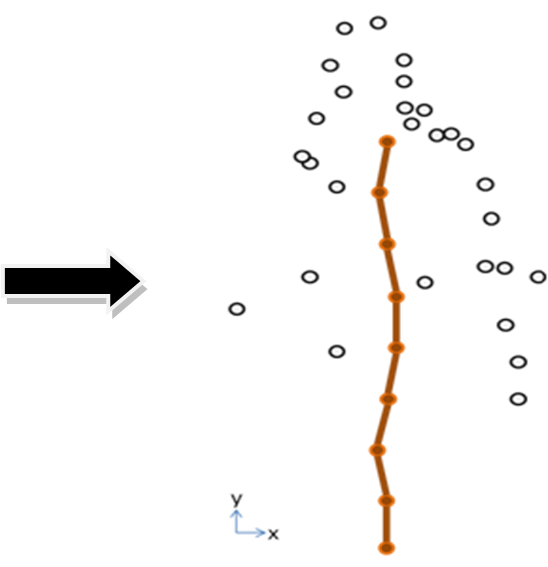
\includegraphics[width=\textwidth]{PineTrunk3}
                \caption{Adding random offsets looks more natural.}
                \label{fig:PineTrunksubfig3}
        \end{subfigure}             
\caption{A simple trunk model is added to the collection of branch tip positions.}
\label{fig:PineTrunk}
\end{figure}

A particle represents a branch tip. One group of particles is 3D positions of branch tips recorded from motion capture, which is described in Section \ref{sec:Dataprocessing}. Figure \ref{fig:PineTrunksubfig1} shows a photograph of a pine tree with markers placed on the crown. All the branch tip locations recorded by motion capture are labeled with white dots. These particles are shown in black circles in Figure \ref{fig:boundboxsubfig3} and Figure \ref{fig:ConvexHullPoints}. 

Because of motion capture's limited capability, we cannot record locations for every branch tip on the tree. Another group of particles is randomly generated within the bounded space of all the recorded branch tip positions. In Figure \ref{fig:boundboxsubfig3} and Figure \ref{fig:ConvexHullPoints}, these particles are green. 

Instead of using one single bounding box for the whole tree crown, we create a vertical stack of bounding boxes as shown in Figure \ref{fig:boundbox}. The new bounding boxes more closely match the tree shape. In Figure \ref{fig:boundboxsubfig3}, the crown height is evenly divided into four parts. Particles are randomly generated inside the smaller bounding boxes, as shown using green dots in Figure \ref{fig:boundboxsubfig3}. The total number of branch tips, including motion capture branch tips and randomly generated particles, is set to be similar to the original tree. The number of green dots in each box is proportional to the number of black dots. Therefore, we maintain a similar total amount and distribution of natural tree branch tips.

\begin{figure}
\centering
        \begin{subfigure}[b]{0.2\textwidth}
                \centering
                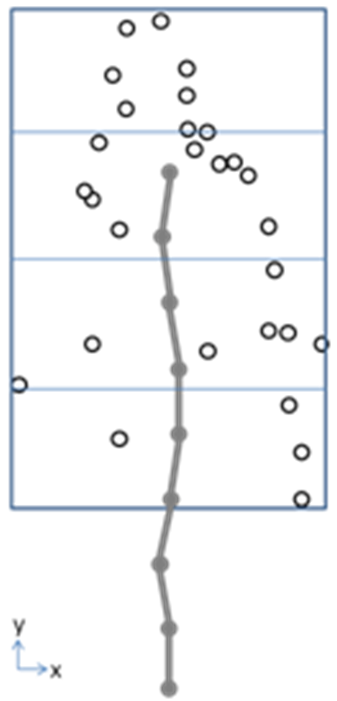
\includegraphics[width=\textwidth]{boundbox1}
                \caption{}
                \label{fig:boundboxsubfig1}
        \end{subfigure}
        ~
        \begin{subfigure}[b]{0.27\textwidth}
                \centering
                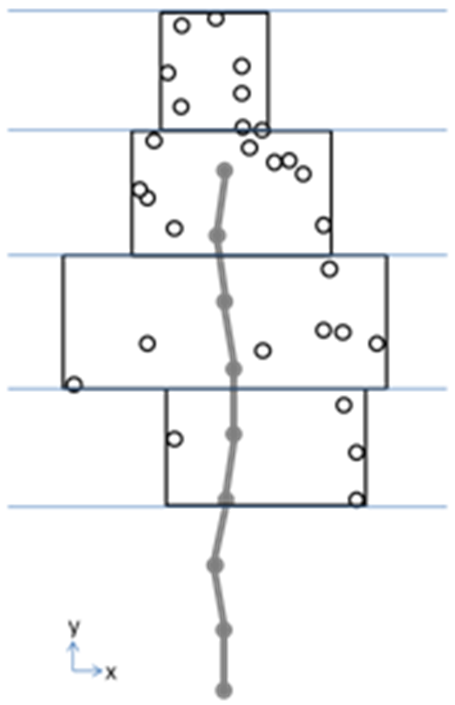
\includegraphics[width=\textwidth]{boundbox2}
                \caption{}
                \label{fig:boundboxsubfig2}
        \end{subfigure} 
        ~
        \begin{subfigure}[b]{0.2\textwidth}
                \centering
                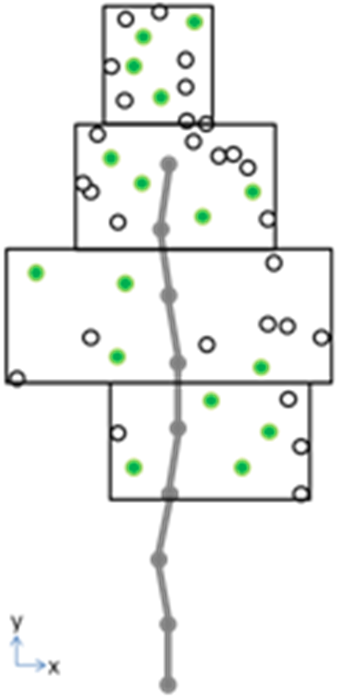
\includegraphics[width=\textwidth]{boundbox3}
                \caption{}
                \label{fig:boundboxsubfig3}
        \end{subfigure}             
\caption{New particles are added within a vertical stack of bounding boxes.}
\label{fig:boundbox}
\end{figure}

Alternatively, we use a convex hull for all the particles, as shown in Figure \ref{fig:ConvexHullPoints}. A convex hull provides more precise bounding space than the stack of bounding boxes. However, it requires a (slightly) more complex boundary detection scheme and more implementation details. Because of the precision that a convex hull brings, we recommend this approach for building a bounding volume.

\begin{figure}[!t]
\centering
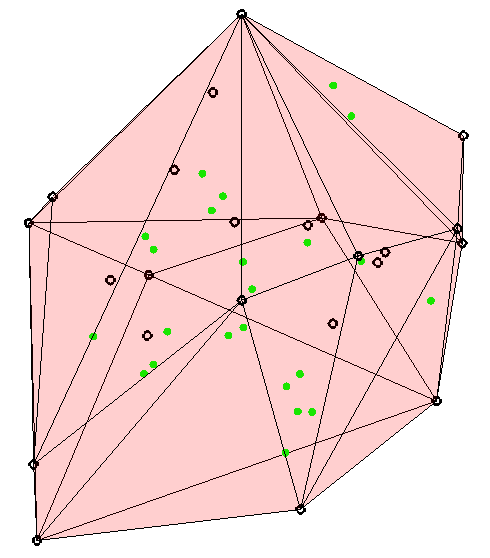
\includegraphics[scale=0.5]{ConvexHullPoints}
\caption[A convex hull for all the particles.]{A convex hull for all the particles. Particles in black color are from motion capture and particles in green color are randomly generated inside the convex hull.}
\label{fig:ConvexHullPoints}
\end{figure}

For the pine tree's trunk, we generate nine nodes in a straight vertical line and add random offsets in the x and z directions to these trunk nodes. The length of the line is scaled about 1.2 times the pine tree's crown height.

Trunk nodes contain a root attractor point and a nearest trunk point, as shown in Figure \ref{fig:flow}. The root attractor point, shown in green, is the trunk node closest to the lower bound of the bounding box for the entire crown. The nearest trunk point, which is shown in blue for the red particle in Figure \ref{fig:flowsubfig1}, is the closest trunk node to a single particle.

\begin{figure}
\centering
        \begin{subfigure}[b]{0.2\textwidth}
                \centering
                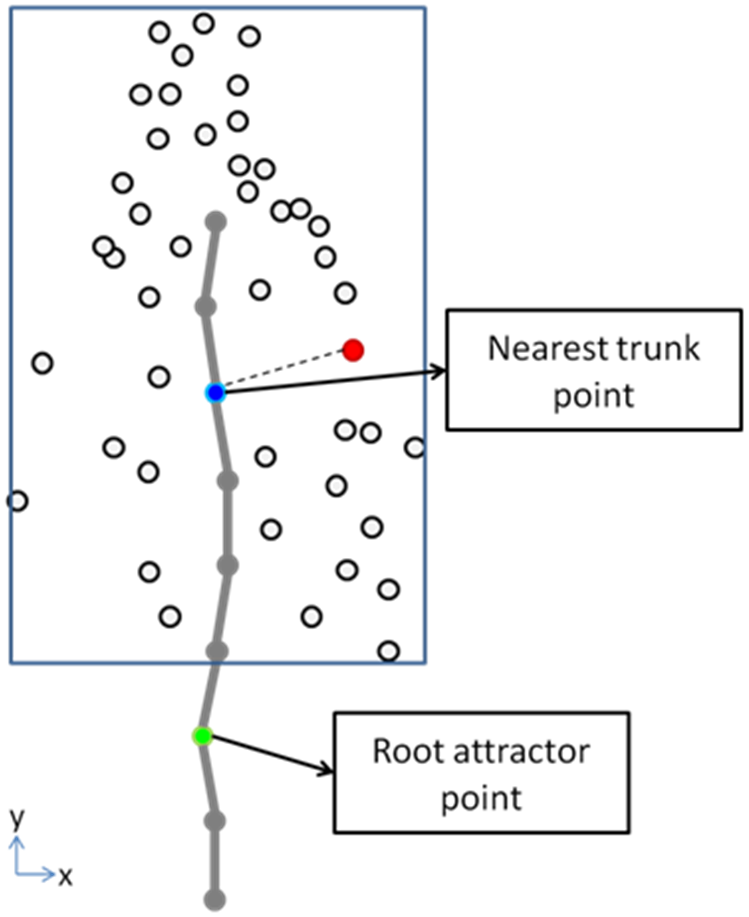
\includegraphics[width=\textwidth]{flow1}
                \caption{Flow direction depends on root attractor and nearest trunk point positions.}
                \label{fig:flowsubfig1}
        \end{subfigure}
        ~
        \begin{subfigure}[b]{0.3\textwidth}
                \centering
                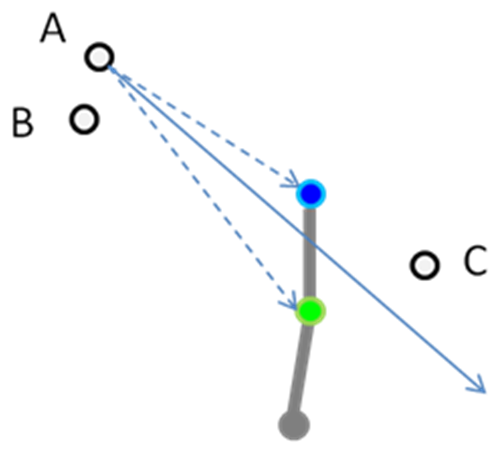
\includegraphics[width=\textwidth]{flow2}
                \caption{Root attractor point $S_r$ and nearest trunk point $S_t$.}
                \label{fig:flowsubfig2}
        \end{subfigure} 
        ~
        \begin{subfigure}[b]{0.3\textwidth}
                \centering
                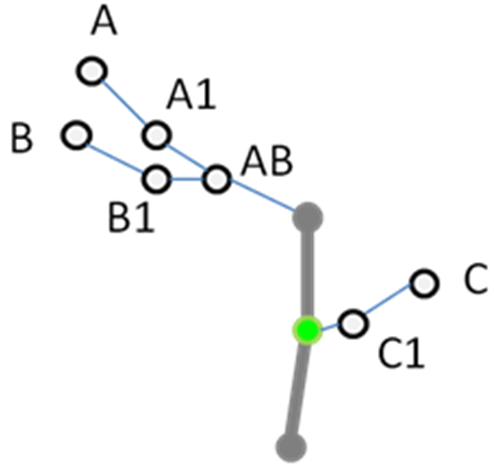
\includegraphics[width=\textwidth]{flow3}
                \caption{Particle flow ends when a particle merges with a neighbor or with the trunk.}
                \label{fig:flowsubfig3}
        \end{subfigure}             
\caption{A simple particle flow results in crown branching structure.}
\label{fig:flow}
\end{figure}

Particles move under directions of three forces: gravity, shape-format, and dominant wind. In Figure \ref{fig:forceTable}, we describe the direction and magnitude of each force. Gravity points vertically down to the ground. We assume that a particle has higher mass when it is closer to the trunk. This assumption follows the observation that when closer to the trunk, a branch has a larger radius. For a particle with higher mass, it has a larger magnitude of gravity and moves faster in the vertical downwards direction. Under this assumption, we set the magnitude of gravity proportional to the distance between a particle position $S_p$ and nearest trunk point $S_t$. 

We call the second force shape-format. Arborists distinguish styles of growth habit of trees using different classifications, such as excurrent and decurrent. The force tries to guide particle flow to follow the growth pattern of the original tree. Simulating different growth patterns requires different definitions of the shape-format force. In this research, we provide a simple example of shape-format definition. The shape-format force, shown in Figure \ref{fig:forceTable}, guides the particle flow process by height and depth of a tree crown. The direction of the force is pointing to the root attractor point $S_r$ from particle location $S_p$. The magnitude of the force is the average height of all the particles with a weight parameter $\alpha$. The higher the center of all the particles, the stronger the shape-format force points to the root attractor point $S_r$. This force is a pre-computed global force, which is a constant for all the particles. The direction of the force ensures that a particle finally merges to trunk nodes, and therefore all the branches grow towards the trunk.

The dominant wind direction is recorded from the motion capture setup, as described in Section \ref{sec:Motioncapturetrees}. Wind force is a special case of external force acting on the tree's branching shapes and structures. While doing motion capture, we record the location of the electrical fan. Because we only use one fan to create wind, that is the only source of explicit external force. Alternatively, the dominant wind direction can be inferred from tree movements recorded in motion capture data. Statistic methods, such as PCA , can estimate the dominate wind direction.

\begin{figure}[!t]
\centering
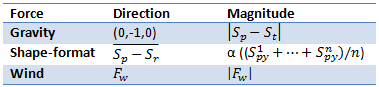
\includegraphics[scale=1.2]{forceTable}
\caption[Definition of three forces. ]{Forces: gravity, shape-format, and dominate wind. 
$S_p$: position of a particle. $S_{py}$ is position of a particle in $y$ direction.
$S_t$: position of the nearest trunk point.
$S_r$: position of the root attractor point.
$F_w$: wind measured from motion capture setup.
$\alpha$: scaling weight in range of [0, 1].
$n$: number of particles.
}
\label{fig:forceTable}
\end{figure}

The flow of particles starts at branch tips. Some particles merge in the flow process while others eventually reach and merge to the trunk. At each time step, we compute for step size and direction of a particle. The step size $L$ is:

\begin{equation}
\label{eqn:model1}
			L = \beta * ||S_p, S_t||,
\end{equation}

where $\beta$ is a tunable parameter in range of [0.1, 0.5] for most of our tree models. The step direction combines all the three forces. Figure \ref{fig:flowsubfig2} shows the computation of the direction for particle $i$, which is shown as particle $A$ in Figure \ref{fig:flowsubfig2}. Each force has a weighting parameter $\omega$ that tunes the relative importance of each vector and provides flexibility in creating branching shapes. The particle step direction $\vec{D_i}$ is given by

\begin{equation}
\label{eqn:model2}
	\vec{D_i} = (\omega_1*\vec{G_i} + \omega_2*\vec{S_i} + \omega_3*\vec{W_i} )/3,
\end{equation}

where $\omega$ is the weight of the direction, $\vec{G_i}$ is direction of gravity, $\vec{S_i}$ is direction of shape-format, and $\vec{W_i}$ is the wind direction for particle $i$ where $i\in[1,...,n]$.

Using step size $L$ and direction $\vec{D}$, the new particle position $V(m)$ is given by

\begin{equation}
\label{eqn:model3}
 V(m) = V(m-1) + L*\vec{D_i},
\end{equation}

where $m$ is current time step and $V(m-1)$ is the particle position at the last time step.

At each time step, after updating all the particle positions, particles might be merged. When the distance between a pair of particles is less than a predefined merging threshold, those particles are combined. When the distance between a particle and a trunk point falls below a predefined merging threshold, that particle is merged with the trunk. In Figure \ref{fig:flowsubfig3}, we demonstrate the paths of particle flow. Particle $A$, $B$, and $C$ are moved using the step and direction. Particle $A$ and $B$ are merged at point $AB$ and finally merged to the trunk. Particle $C$ merged to the trunk point after two time steps of movement.

\section{Adding Leaves}

Tree leaves are visually important to 3D tree models. After the branching structure is generated, leaves are attached. We use predefined leaf shapes, growth patterns, densities, and sizes. Also, because leaves do not always start growing at the beginning of a branch, we set a parameter called the leaf starting point. This parameter is proportional to a branch length. For example, when the parameter is $0.3$, it starts leaves after the point that is $0.3$ times the branch length away from the branch starting point. 

\section{Results}

Results are given for multiple trees, including maple and pine trees. The maple tree is instrumented with 24 markers placed on the periphery of the crown at branch tips and the pine tree is instrumented with 35 markers also located on branch tips. We collect the stationary locations of these markers for about 20 seconds at the capture rate of 100 frames/sec.

Figure \ref{fig:clustersubfig1} shows all the recorded locations as red dots for a single frame, and Figure \ref{fig:clustersubfig2} shows averaged locations from each cluster of marker positions for clusters in which the number of frames with a position in that cluster is $1/4$ of the total frame count. The data is recorded when the tree is stationary. Notice that a point in the blue box in Figure \ref{fig:clustersubfig1} is identified as noise and removed by the clustering algorithm. For the maple tree, after clustering and averaging only 24 markers remain and this matches the actual number of markers placed on the tree.

\begin{figure}
\centering
        \begin{subfigure}[b]{0.4\textwidth}
                \centering
                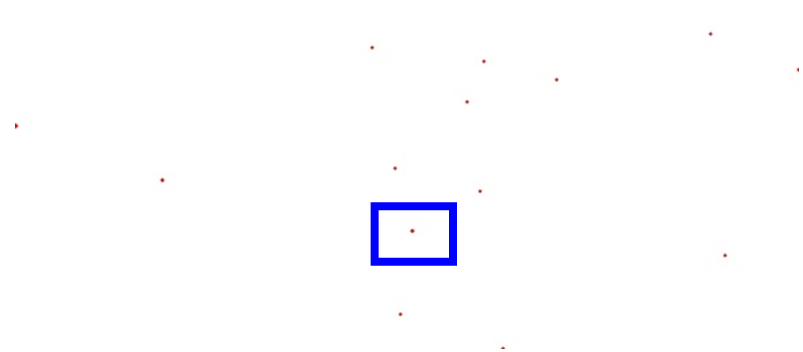
\includegraphics[width=\textwidth]{cluster1}
                \caption{Original collected data.}
                \label{fig:clustersubfig1}
        \end{subfigure}
        ~
        \begin{subfigure}[b]{0.4\textwidth}
                \centering
                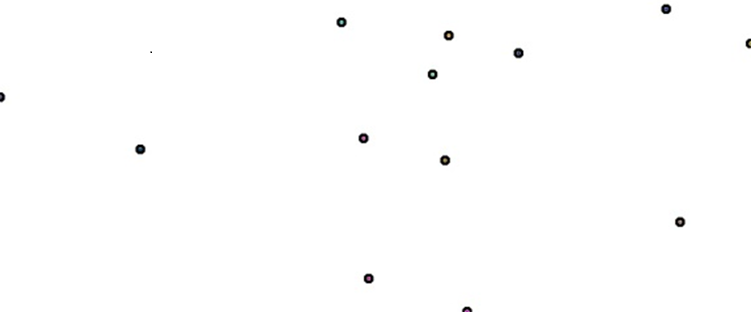
\includegraphics[width=\textwidth]{cluster2}
                \caption{Remaining branch tip locations after clustering.}
                \label{fig:clustersubfig2}
        \end{subfigure}     
        \caption{Clustering that removes noise that leads to spurious marker positions.}
        \label{fig:cluster}
\end{figure}

Although initial marker positions are collected before wind is applied when the tree is stationary, the data contain a small amount of noise, which can be removed to create a single initial marker position. In Figure \ref{fig:markerPath}, we show marker positions over time for two markers during the stationary phase. The horizontal axis shows time while the vertical axis shows a marker location in 3D space. In the first image, movement in each direction spans $10^{-3}$ meters. In addition, in the second image there is apparently a small periodic motion for the stationary branch tip. The range of motion is also within $10^{-3}$ meters. In both cases, averaging removes this small motion and estimates initial marker positions based on the average rather than a single position in a single frame.

\begin{figure}
\centering
        \begin{subfigure}[b]{0.42\textwidth}
                \centering
                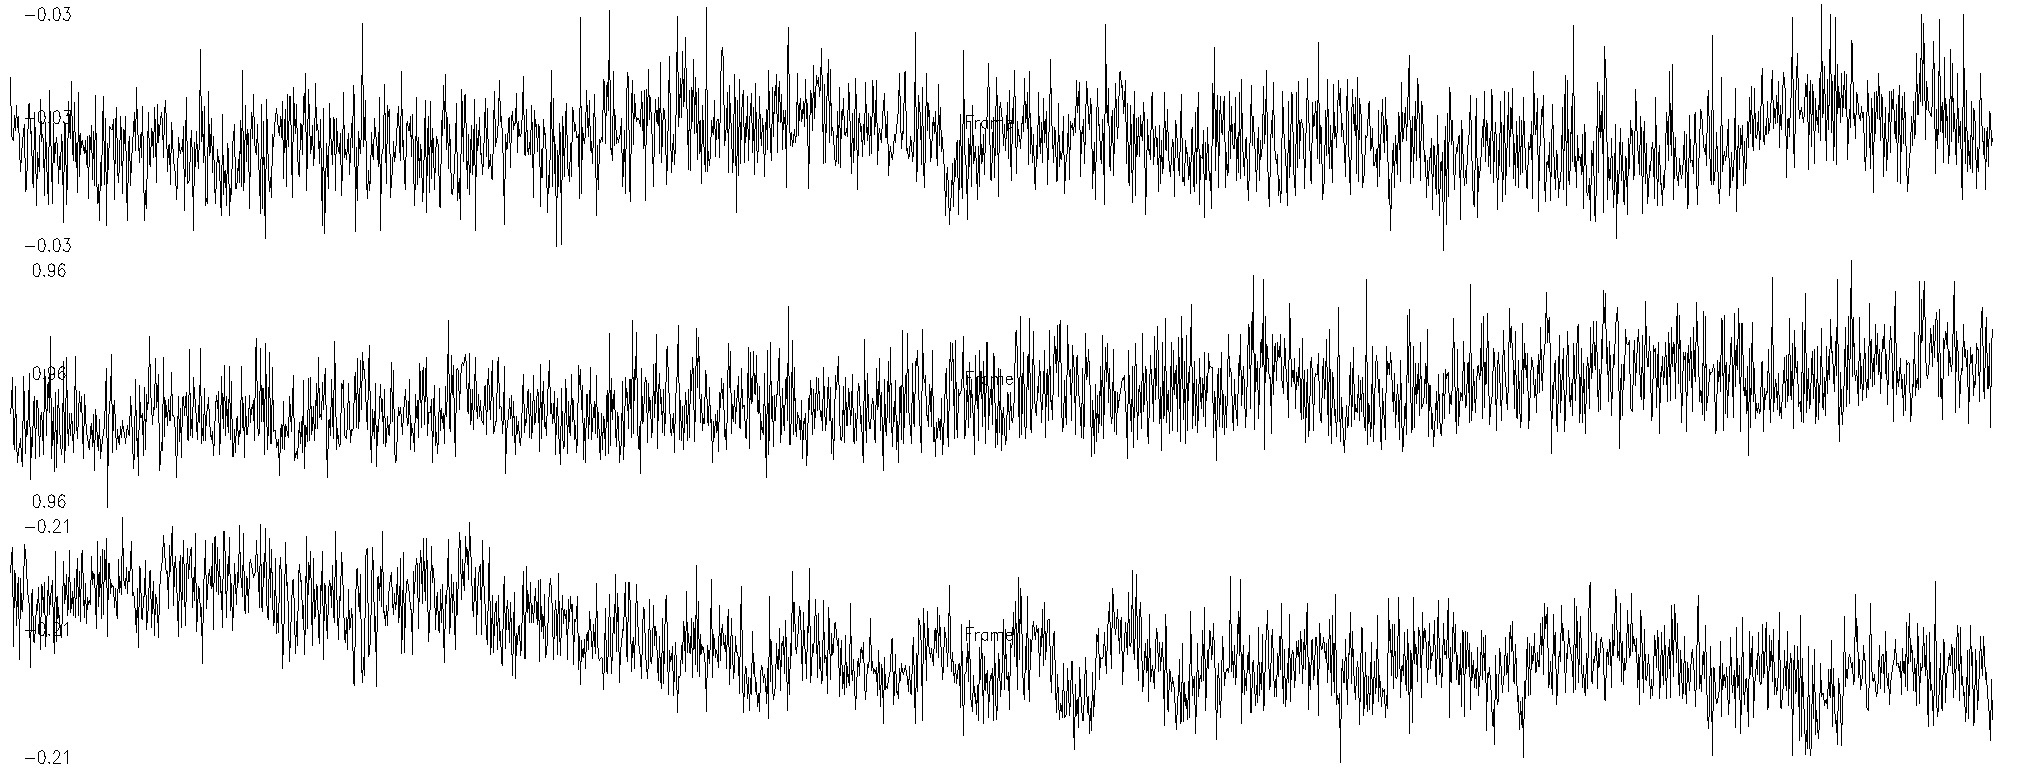
\includegraphics[width=\textwidth]{Marker0orig}
                \caption{Close to white noise.}
                \label{fig:markerPathsubfig1}
        \end{subfigure}
        ~
        \begin{subfigure}[b]{0.42\textwidth}
                \centering
                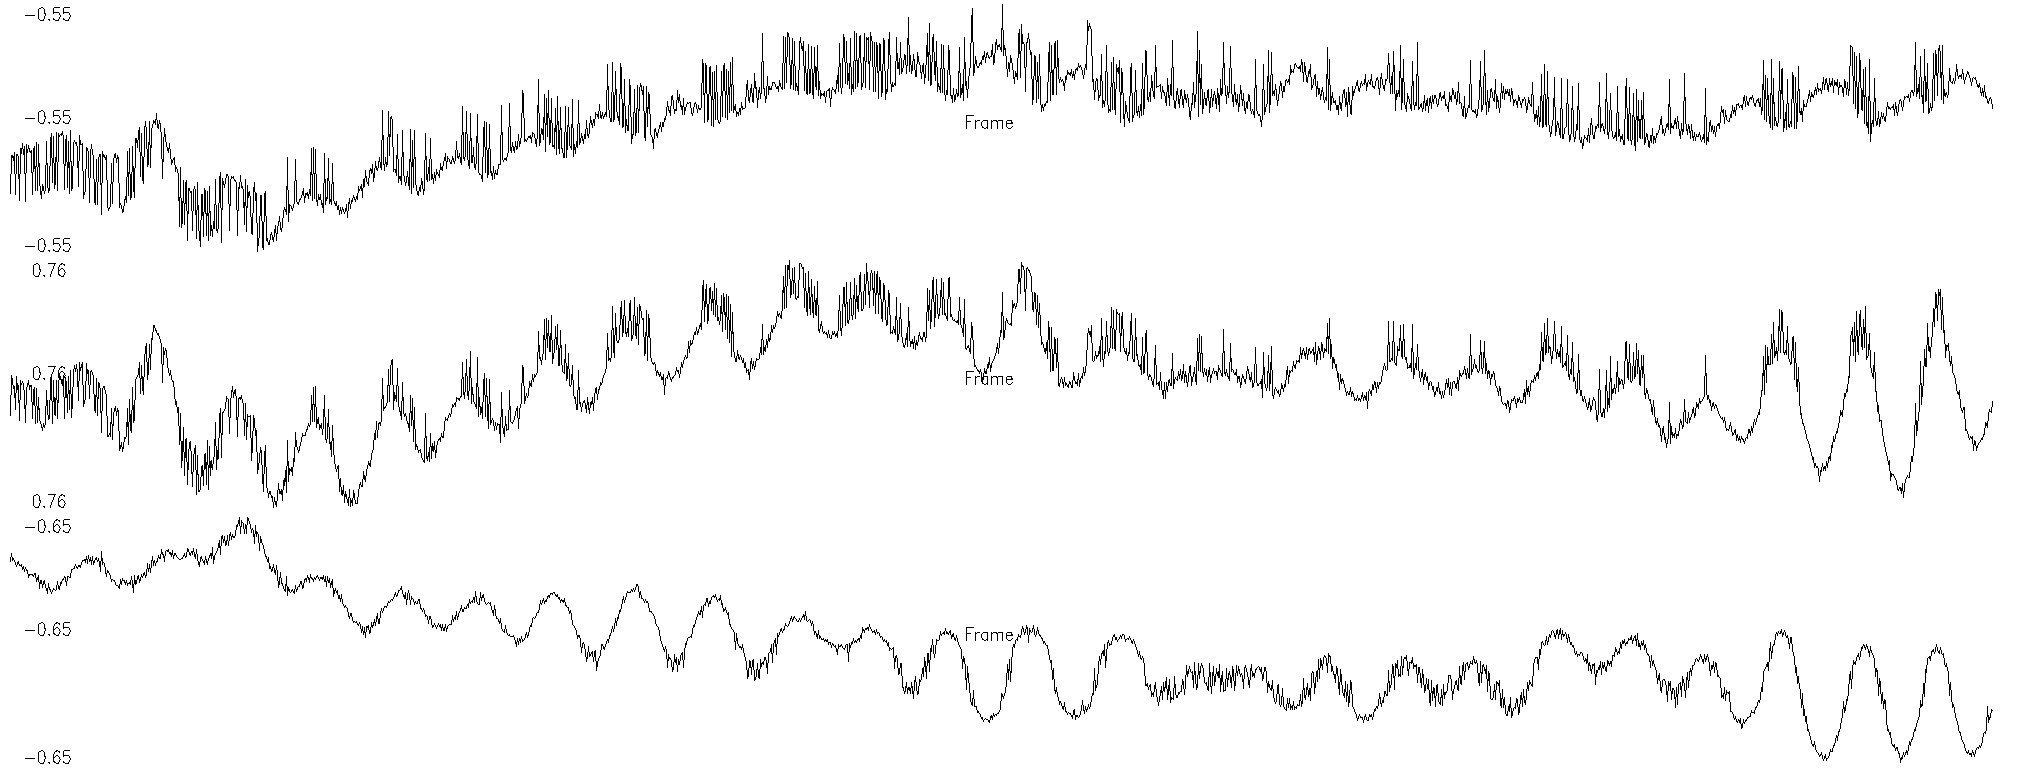
\includegraphics[width=\textwidth]{Marker5orig}
                \caption{Noise with apparent periods.}
                \label{fig:markerPathsubfig2}
        \end{subfigure}     
        \caption[Remove spurious motion. ]{Marker positions over time contain a small amount of spurious motion that is removed by averaging.}
        \label{fig:markerPath}
\end{figure}

A vertical stack of bounding boxes is a better approximation for the crown volume than a single bounding box and results in better crown shapes. Each bounding box contains branch tips and additional branch tips are added to each box. Figure \ref{fig:boundboxsizesubfig1} and Figure \ref{fig:boundboxsizesubfig2} illustrate the difference between tree crowns created with and without a stack of bounding boxes for a pine tree. Random particles placed uniformly within a single bounding box result in a cube shaped tree. Placing particles in a vertical stack of bounding boxes better approximates the original crown shape. Future work might include investigating non-uniform distributions of randomly inserted points instead of using bounding boxes. 

In Figure \ref{fig:boxTree} and Figure \ref{fig:convextTree}, we demonstrate the difference between tree shapes using stacked box bounding volumes and those using convex hull bounding volumes. The bounding box approach provides a looser bounding condition and allows more random factors in the final tree shape. The convex hull approach more closely approximates the original tree crown shape.

\begin{figure}
\centering
        \begin{subfigure}[b]{0.33\textwidth}
                \centering
                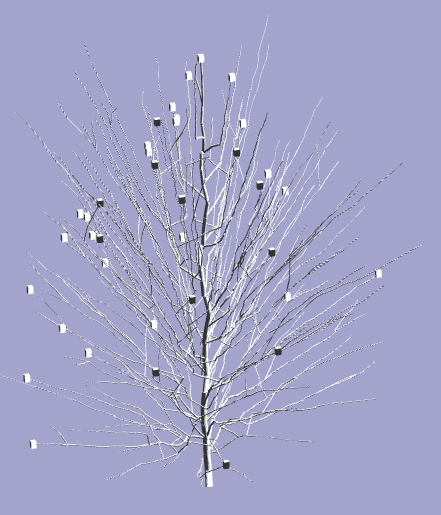
\includegraphics[width=\textwidth]{ResultBoundPine2}
                \caption{}
                \label{fig:boundboxsizesubfig1}
        \end{subfigure}
        ~
        \begin{subfigure}[b]{0.34\textwidth}
                \centering
                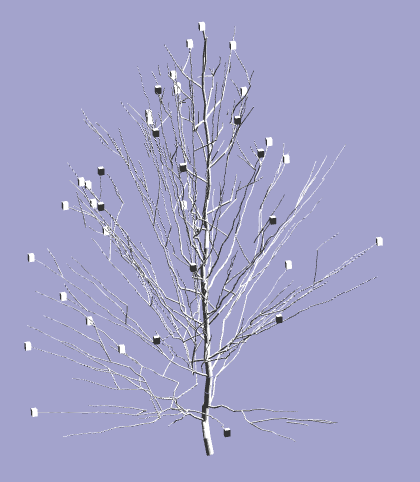
\includegraphics[width=\textwidth]{ResultBoundPine1}
                \caption{}
                \label{fig:boundboxsizesubfig2}
        \end{subfigure}
        ~
        \begin{subfigure}[b]{0.34\textwidth}
                \centering
                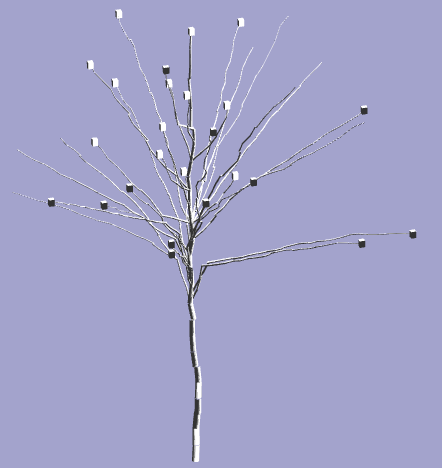
\includegraphics[width=\textwidth]{boundBoxTree}
                \caption{}
                \label{fig:boxTree}
        \end{subfigure}
        ~
        \begin{subfigure}[b]{0.33\textwidth}
				        \centering
				        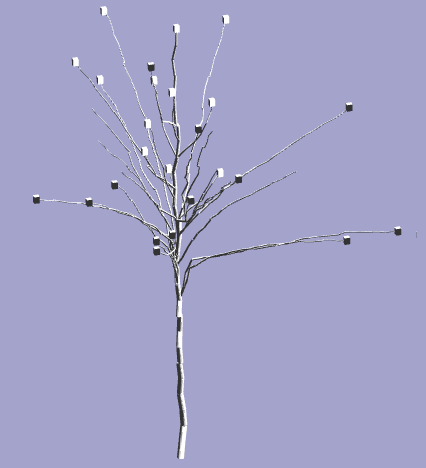
\includegraphics[width=\textwidth]{boundConvexTree}
				        \caption{}
				        \label{fig:convextTree}
        \end{subfigure}
\caption{Bounding volumes affect tree shape.}
\label{fig:boxConvex}
\end{figure}

Particle flow starting from branch tips and using our simplified algorithm results in tree crown shapes that mimic the shape of the tree from which data were collected. In the Figure \ref{fig:treemodelssubfig1}, we show the results from reconstructing a pine tree. 

\begin{figure*}[!t]
\centering
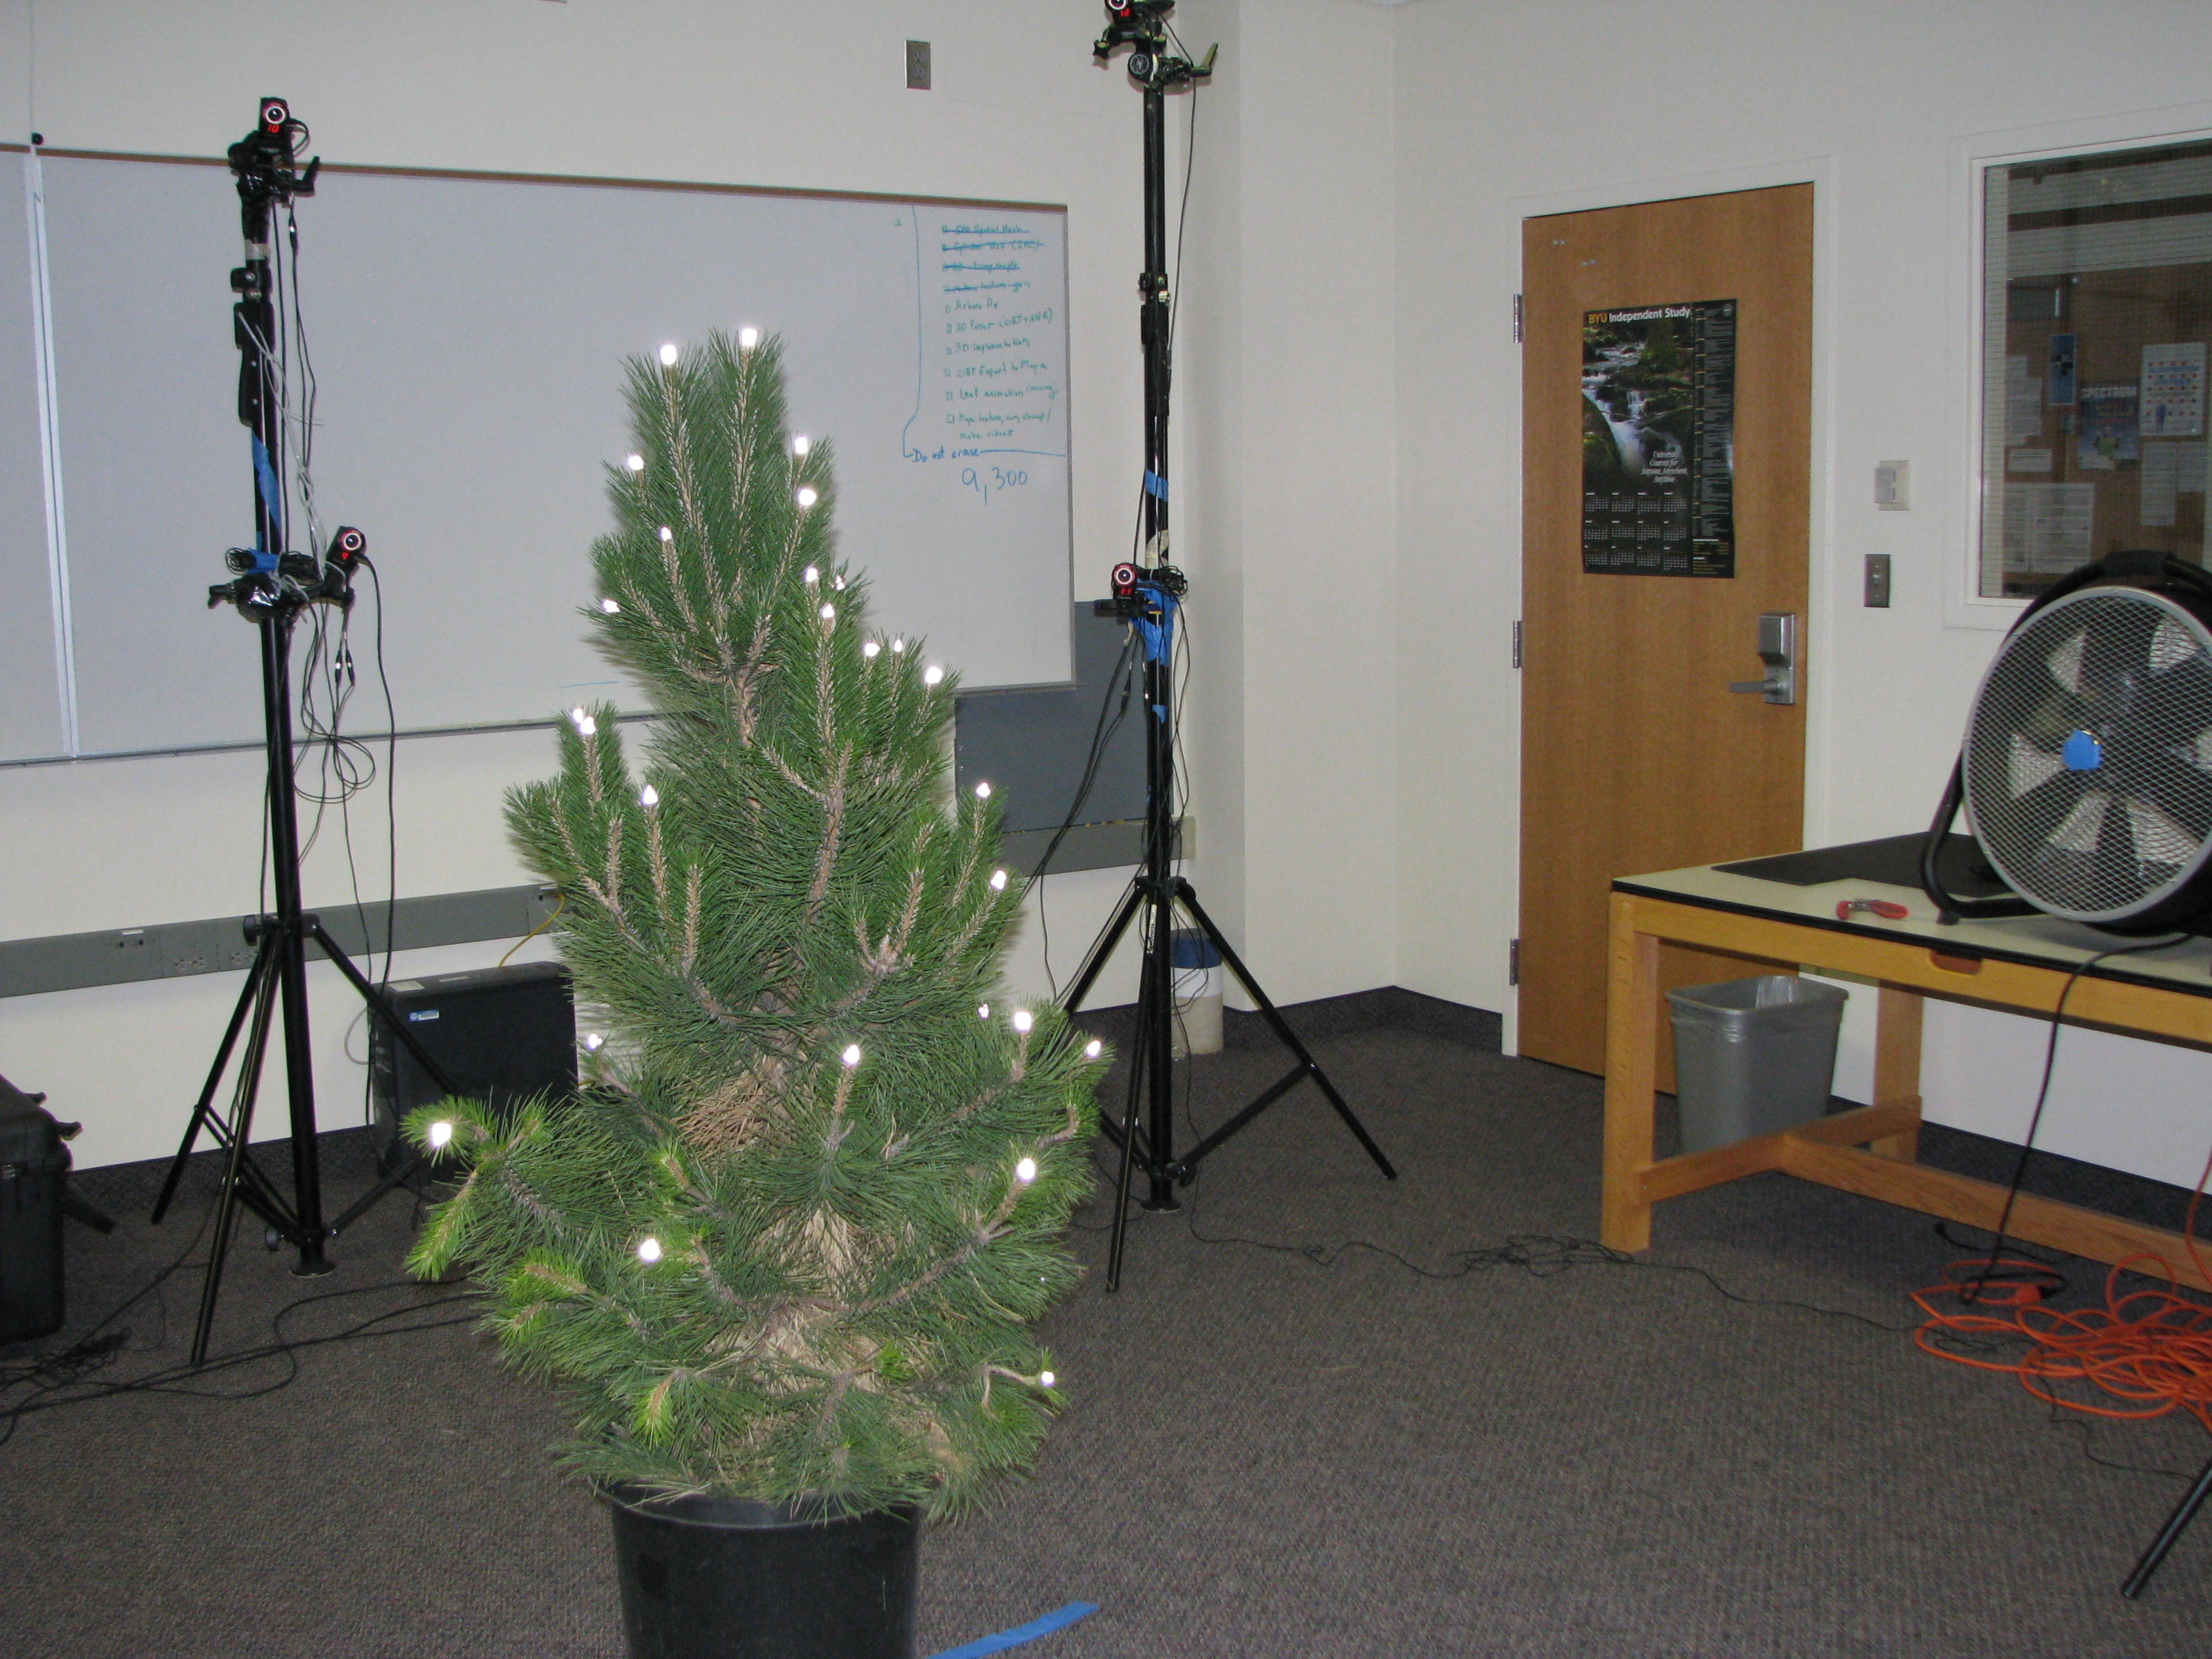
\includegraphics[scale=0.36]{Pine}
\caption[Pine tree model.]{Pine tree model. 3D tree models created from branch tip positions are similar to the shapes of the trees from which branch tip positions were collected.}
\label{fig:treemodelssubfig1}
\end{figure*}

Besides replaying the original tree shape, our approach has enough flexibility to produce different tree shapes based on the same set of motion capture data. Three forces with their scales create particles' moving paths, which represents branching structures. Figure \ref{fig:currency} demonstrates that shape-format force sets the global attracting trunk node, which controls the converging direction of particle flow. The resulting tree models display trees' growth styles in terms of excurrent and decurrent.

\begin{figure}
\centering
        \begin{subfigure}[b]{0.33\textwidth}
                \centering
                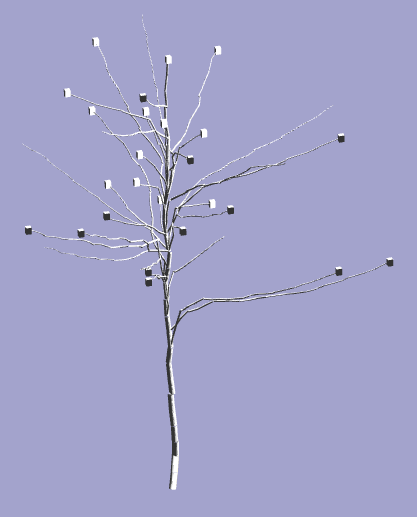
\includegraphics[width=\textwidth]{currency1}
                \caption{}
                \label{fig:currency1}
        \end{subfigure}
        ~
        \begin{subfigure}[b]{0.33\textwidth}
                \centering
                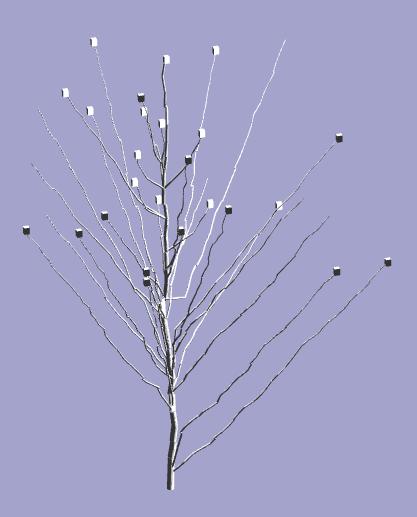
\includegraphics[width=\textwidth]{currency2}
                \caption{}
                \label{fig:currency2}
        \end{subfigure}
\caption{Shape-format force.}
\label{fig:currency}
\end{figure}

Figure \ref{fig:gravityTree} shows the impact of gravity on trees' shapes with various values for the weighting factor. When the factor is set to be negative, we create a special willow-like tree shape. 

\begin{figure}
\centering
        \begin{subfigure}[b]{0.3\textwidth}
                \centering
                \includegraphics[width=\textwidth]{gravity001}
                \caption{weighting factor: 0.01}
                \label{fig:gravity001}
        \end{subfigure}
        ~
        \begin{subfigure}[b]{0.3\textwidth}
                \centering
                \includegraphics[width=\textwidth]{gravity020}
                \caption{weighting factor: 0.20}
                \label{fig:gravity020}
        \end{subfigure}
        ~
        \begin{subfigure}[b]{0.3\textwidth}
                \centering
                \includegraphics[width=\textwidth]{gravityNeg020}
                \caption{weighting factor: -0.20}
                \label{fig:gravityNeg020}
        \end{subfigure}
\caption{Tree shapes with different weight factors for gravity.}
\label{fig:gravityTree}
\end{figure}

Figure \ref{fig:windFactor} shows tree models with different weighting factors of wind force. Bigger values of the factor produces branches bending more toward the wind direction. Notice that the differences among these tree models are small, especially when compared to the influence from the other two forces. This is because the value of force for a global wind direction is set to be much smaller than that of the other two forces. Otherwise, when wind force dominates the direction of particle movement, the particles might not be able to merge to a tree's trunk and might violate natural tree's shape. 

\begin{figure}
\centering
        \begin{subfigure}[b]{0.3\textwidth}
                \centering
                \includegraphics[width=\textwidth]{wind001}
                \caption{Weighting factor: 0.01.}
                \label{fig:wind001}
        \end{subfigure}
        ~
        \begin{subfigure}[b]{0.3\textwidth}
                \centering
                \includegraphics[width=\textwidth]{wind007}
                \caption{Weighting factor: 0.07.}
                \label{fig:wind007}
        \end{subfigure}
        ~
        \begin{subfigure}[b]{0.3\textwidth}
                \centering
                \includegraphics[width=\textwidth]{wind015}
                \caption{Weighting factor: 0.15.}
                \label{fig:wind015}
        \end{subfigure}
\caption{Tree shapes with different weighting factors for wind force.}
\label{fig:windFactor}
\end{figure}

In Figure \ref{fig:moreShapes}, we generate 3D tree models with different parameters for particle flow with the same set of motion capture data. These results demonstrate that our approach produces visually plausible tree shapes, which becomes scalable for more extended shapes through tweaking parameters of the three forces. 

\begin{figure}
\centering
        \begin{subfigure}[b]{0.3\textwidth}
                \centering
                \includegraphics[width=\textwidth]{treediff1}
                \caption{}
                \label{fig:treediff1}
        \end{subfigure}
        ~
        \begin{subfigure}[b]{0.3\textwidth}
                \centering
                \includegraphics[width=\textwidth]{treediff2}
                \caption{}
                \label{fig:treediff2}
        \end{subfigure}
        ~
        \begin{subfigure}[b]{0.3\textwidth}
                \centering
                \includegraphics[width=\textwidth]{treediff3}
                \caption{}
                \label{fig:treediff3}
        \end{subfigure}
\caption{Various tree shapes.}
\label{fig:moreShapes}
\end{figure}

\section{Discussion and Future Work}

Placing retroreflective markers on branch tips evenly spaced throughout the crown on trees located in a passive optical motion capture arena results in data that can be used to reconstruct tree shape and which may be usable for replaying branch motion.  This can be done using a simplified particle flow system starting from recorded branch tip positions supplemented with additional random branch tip positions within a horizontal stack of bounding boxes and by setting two control parameters.  A new data collection process designed for trees may extend the use of motion capture to include trees and eventually other networks of non-rigid bodies. 

Future work includes extending the process to large trees outdoors as well as improving methods for animating the resulting tree models using the motion capture data.   We have reconstructed an approximate tree crown branching structure.  Replaying the captured motion data will require care to ensure that the motion of the approximate branching structure does not include uncorrelated motion for branch tips who share a common parent.
\chapter[Paper: Hierarchical Heuristic Search Using A Gaussian Mixture Model for UAV Coverage Planning]{Paper: Hierarchical Heuristic Search Using A Gaussian Mixture Model for UAV Coverage Planning\footnote {Submitted to SMC-B (IEEE Transactions On Systems, Man And Cybernetics Part B, Cybernetics) journal and under 3rd round of review. Authors are Lanny Lin, and Michael A. Goodrich.}}
\label{chap:SMCB2014}

\begin{abstract}
During UAV search missions, efficient use of UAV flight time requires flight paths that maximize the probability of finding the desired subject. The probability of detecting the desired subject based on UAV sensor information can vary in different search areas due to environment elements like varying vegetation density or lighting conditions, making it likely that the UAV will only be partially able to detect the subject. This adds another dimension of complexity to the already difficult (NP-hard) problem of finding an optimal search path. We present a new class of algorithms that account for partial detection in the form of a task difficulty map and produce paths that approximate the payoff of optimal solutions. The algorithms use the \textit{Mode Goodness Ratio} heuristic, which uses a Gaussian Mixture Model to prioritize search subregions. The algorithms search for effective paths through the parameter space at different levels of resolution. We compare the performance of the new algorithms against two published algorithms (Bourgault's algorithm and LHC-GW-CONV algorithm) in simulated searches with three real search and rescue scenarios, and show that the new algorithms outperform existing algorithms significantly and can yield efficient paths that yield payoffs near the optimal.  
\end{abstract}


%\begin{IEEEkeywords}
%Unmanned aerial vehicles, path planning, navigation, hierarchical systems, heuristic algorithms
%\end{IEEEkeywords}
%
%\IEEEpeerreviewmaketitle

%=================================================================================
\section{Introduction}
\label{sec:Introduction}

%\IEEEPARstart

Mini-UAVs (Unmanned Aerial Vehicles) are becoming useful tools in many reconnaissance, remote-sensing, surveillance, and search operations thanks to advances in UAV technologies. They can help firefighters map forest fires, help news crews provide coverage, help police monitor crowds, and help wilderness search and rescue workers locate a missing person. In these applications, the UAV uses its on-board cameras to provide useful visual information in support of the specific operation.

This paper focuses on using mini-UAVs to support Wilderness Search and Rescue (WiSAR). The aerial view from a UAV enables WiSAR workers to survey large areas of importance in real time~\cite{Goodrich2008Supporting}. Search efficiency is very important in WiSAR because, as time progresses, the survivability of the missing person decreases and the effective search radius increases by approximately 3km/hour~\cite{Syrotuck2000Introduction}. Therefore, a good flight path should rapidly maximize the probability of finding the missing person to make efficient use of the limited flying time.

Each UAV path accumulates information over time as the UAV's sensors scan the ground. As illustrated in Fig.\ref{TwoApproaches}, various paths do so in different ways depending on how information is distributed in the environment. The goal is to maximize the total probability of detection. There are two quality metrics for the probability-maximizing path planning problem~\cite{Koopman1957Theory, Stone1975Theory, Washburn1981Search}. First, find the path that maximizes the Cumulated Detection Probability (CDP) after a specific flight time (blue vertical dotted line). Out of the three example paths in Fig.
\ref{TwoApproaches} path 3 becomes the winner. Second, find the path that achieves a desired CDP in the shortest amount of time (red horizontal dotted line). Path 1 would become the winner out of the three, instead. We model the problem following the first approach.
\begin{figure}
\centering
\includegraphics[width=3.0in]{Approaches.jpg}
\caption{Two approaches to the probability-maximizing path planning problem. With three paths generated by various algorithms, the first approach prefers the path maximizing the Cumulated Detection Probability (CDP) given a specific flight time (Path 3 is the winner) and the second approach prefers the path achieving a specified CDP in the shortest amount of time (Path 1 is the winner)}. 
\label{TwoApproaches}
%\vspace*{-3ex}
\end{figure}

When using a UAV's on-board camera to assist WiSAR operations, factors such as dense vegetation, lighting conditions, shadows, or distance between the camera and the ground can lower the quality of the UAV aerial view and decrease the probability of detection~\cite{Morse2010UAV}. This can be attributed to both sensor and human limitations (such as limited attention span and cognitive workload). We propose to represent \textit{partial detection} in the form of a task difficulty map, where a more difficult subregion on the map has lower probability of detection. Using a task difficulty map enables us to integrate geo-referenced and spatial-related sensor constraints into the problem formulation, which supplements traditional sensor modeling methods (e.g.,~\cite{Bourgault2006Optimal}) and potentially improves search performance in real world search scenarios. Because detection difficulties vary in different search subregions, flying patterns such as lawnmower and Zamboni don't guarantee optimal coverage. Integrating the task difficulty map into path planning adds another dimension of complexity to the already difficult problem and causes the performance of existing greedy-type algorithms (Bourgault's Algorithm~\cite{Bourgault2006Optimal} and LHC-GW-CONV~\cite{Lin2009UAV}) to suffer.

We model the path planning problem as a discrete combinatorial optimization problem, and propose a new heuristic, the \textit{Mode Goodness Ratio}. This heuristic uses a Gaussian Mixture Model to identify and prioritize search subregions. We then present two new algorithms (\textit{Top2} and \textit{TopN}) that utilize the heuristic in hierarchical path planning by forcing the UAV to visit high priority subregions. The hierarchical structure enables the algorithms (a) to cluster probability volumes and (b) to prioritize search subregions at different levels of resolution. It also makes it easy to parallelize the two new algorithms and improve computation speed. We compare the performance of the new algorithms against two published algorithms (Bourgault's Algorithm~\cite{Bourgault2006Optimal} and LHC-GW-CONV algorithm~\cite{Lin2009UAV}) in simulated searches based on three real search and rescue scenarios. Results show that the new algorithms outperform existing algorithms significantly and can yield efficient paths that approximate the payoff of the optimal path.

The contributions of the paper are (a) the introduction of Gaussian Mixture Model (GMM) to compute the Mode Goodness Ratio heuristic, which can be used to prioritize search subregions in a hierarchical planner, (b) two new path planning algorithms that utilize the Mode Goodness Ratio heuristic to improve path-planning performance, and (c) the use of a spatial representation (task-difficulty map) in modeling sensor detection probability with terrain and vegetation information and incorporating that into UAV path planning.

Section~\ref{sec:ProblemFormulation} defines the problem and the metrics used to evaluate algorithm performance. Section~\ref{sec:RelatedWork} discusses related literature. Section~\ref{sec:PathPlanningAlgorithms} first reviews two existing algorithms and then demonstrates the weakness of these algorithms with a synthetic scenario. This section then presents the \textit{Mode Goodness Ratio} heuristic and the two new algorithms (\textit{Top2} and \textit{TopN}). Section~\ref{sec:ExperimentResultsAndAnalysis} compares algorithm performance with three real search and rescue scenarios. Section~\ref{sec:LimitationsAndDiscussion} discusses the limitations of the approach, and Section~\ref{sec:Summary} presents the summary.


%=================================================================================
\section{Problem Formulation}
\label{sec:ProblemFormulation}

%=============================
\subsection{Problem Framework}

Typical UAVs (fixed-wing or rotorcraft) are highly mobile and variable, but we will assume a set of useful constraints on their capabilities: they have a gimbaled camera, can maintain a constant height above ground and can travel at constant speed. A gimbaled camera enables the camera to aim straight down even when the UAV is performing roll or yaw maneuvers. We assume that the UAV's speed is much higher than the speed of the missing person and treat the missing person as stationary. At every UAV flight time step, we treat the camera footprint of the search area as a glimpse. This way we can discretize the search area, and model the UAV path planning problem as a discrete combinatorial optimization problem with respect to probability accumulated and define it following the framework described in~\cite{Trummel1986Technical}.

The search space is represented as a finite, connected graph $G = (V, E)$. $V$ denotes the set $\{v_1, ..., v_n\}$ of vertices of $G$, and $E$ denotes the set of edges. Each edge in $E$ can be viewed as an unordered pair of vertices $\{v_i, v_j\}$. The missing person is located at one of the vertices of $G$. A given probability distribution map for the missing person is discretized to match graph $G$, with $p_i$ being the probability that the missing person is located at vertex $v_i$. It is obvious that
\begin{equation}
\sum_{i=1}^{n}p_i = 1.
\label{totalP}
\end{equation}

The UAV search is conducted in discrete time. During each time step, the UAV camera footprint can cover one vertex. For a desired flight with $T$ time steps, let $S$ denote the set $\{0,1,2,...,T\}$. The UAV's motion is constrained by the structure of the graph $G$. Let $\Psi$ be the set of functions $\psi:S \mapsto V$ with the property that for any two consecutive integers $t$ and $t+1$ in $S$, either $\psi(t)=\psi(t+1)$ or $\{\psi(t),\psi(t+1)\}\in E$. Here $\Psi$ represents all possible paths, and under path $\psi$, vertex $\psi(t)$ is searched during step $t$. The conditions on the set $\Psi$ guarantee that at each time step the UAV camera footprint will either remain at the current vertex (only possible for a rotorcraft) or move to a neighboring vertex.

Even when the UAV camera footprint covers the vertex occupied by the missing person, it is not certain that a detection will occur. The probability of detection is described by a glimpse probability function $g$, which is defined by a given task difficulty map. The task difficulty map is a spatial representation of sensor detection probability and defines areas where it is difficult to detect the missing person (with lower probability of detection), with $d_i$ being the task difficulty level at vertex $v_i$. Let $d_{max}$ be the maximum task difficulty level in the given map. If at time step $t$ the UAV camera footprint covers vertex $v$, then let $g(v,t)$ be the probability that a detection will occur, given that the missing person is at vertex $v$. We model this as
\begin{equation}
g(v_i,t) = 1 - \frac{d_i}{d_{max}+1}.
\label{g}
\end{equation}
so that more difficult tasks (higher $d_i$ values) have lower glimpse detection values, $g$.

Let $P_T(\psi)$ represent the Cumulative Detection Probability (CDP) for path $\psi \in \Psi$ with $T$ time steps. For each (cell, time) pair $(i,t)$ with $1 \leq i \leq n$ and $0 \leq t \leq T$, we define the probability of failure $f(i,t,\psi)$ by 
\begin{equation}
f(i,t,\psi) = 
	\left\{
	\begin{array}{ll}
		1-g(v_i,t) & \mbox{if~} \psi(t)=v_i \\
		1 & \mbox{otherwise.}
	\end{array}
	\right.
\label{OneVertex}
\end{equation}
Let $D_j$ represent a detection on the $j$th observation so $\overline{D}_j$ is a detection failure. Then the probability of failing to detect the the missing person after $N$ observations of vertex $v_i$ given the missing person is at vertex $v_i$ is the joint probability $P(\overline{D}_1, \overline{D}_2, ..., \overline{D}_N|v_i)$. Assuming each observation is conditionally independent of each other (typical in the WiSAR literature), we can rewrite the joint probability as
\begin{equation}
P(\overline{D}_{1:N}|v_i) = \prod_{j=1}^{N}P(\overline{D}_j|v_i),
\label{NoDetection}
\end{equation}
and the probability of detecting the missing person after $N$ observations is
\begin{equation}
P(D_{1:N}|v_i) = 1 -  P(\overline{D}_{1:N}|v_i),
\label{Detection}
\end{equation}
which is equivalent to
\begin{equation}
P(D_{1:N}|v_i) = 1 -  \prod_{t=0}^{T}f(i,t,\psi),
\label{Detection2}
\end{equation}
where $N$ is how many times $v_i$ shows in path $\psi$. Then $P_T(\psi)$ can be computed by
\begin{equation}
P_T(\psi) = \sum_{i=1}^{n}p_i\Big(1 - \prod_{t=0}^{T}f(i,t,\psi)\Big),
\label{CDP}
\end{equation}
where $p_i$ is the probability that the missing person is located at vertex $v_i$. Define $\exists\psi^* \!{\in} \Psi$ such that for any alternate path $\psi' \!{\in} \Psi, P_T(\psi^*) \!{\geq} P_T(\psi')$. Our goal is to find the optimal path $\psi^*$ that produces the maximum CDP (path 3 in~Fig.\ref{TwoApproaches} at $T=600$ if there are only three possible paths) or find an efficient path $\psi'$ that produces payoff approximating the payoff of the optimal path within reasonable computation time.

When the path needs to end at an operator-specified vertex (for easy UAV retrieval or to join with other path segments), we simply add the constraint to the problem formulation (only add edges to a path that does not violate the constraint so the UAV has enough time to reach the end point). Also for fixed-wing UAVs, additional motion constraints (such as not allowing the UAV to fly backward) are also introduced as velocity constraints affecting edges $\{\psi(t), \psi(t_1)\}$, effectively creating a directed graph. Both proposed path planning algorithms satisfy these constraints.

%=============================
\subsection{Performance Metrics}

%Let $\mathit{Efficiency_{LB}}$ (Efficiency Lower Bound) and algorithm Run Time producing path $\psi'$ denote metrics to measure the performance of the algorithms. 
We will use two measures of algorithm performance: the quality of the path and the run-time of the algorithm. Run-time is self-explanatory, but we need a measure of path quality. Ideally the efficiency of an algorithm should be computed with the following equation:
\begin{equation}
\mathit{Efficiency}(\psi') = \frac{P_T(\psi')}{P_T(\psi^*)},
\label{Efficiency}
\end{equation}
where $\psi^*$ is the optimal path. However, because we do not know what $\psi^*$ is, we bound the efficiency. Let $\psi_{teleport}$ be defined as the path constructed as follows: (a) deduct the time needed to move from the start vertex to the nearest vertex with non-zero $p_i$ (plus time for doing the same with the end vertex if specified), and (b) at each step the UAV teleports to the vertex that allows the UAV to collect the highest amount of probability after considering the task difficulty at that vertex. Then, all the probability collected during the teleport flight is summed, giving $\mathit{Efficiency_{LB_i}}$ for path $i$:
\begin{equation}
\mathit{Efficiency_{LB_i}} = \frac{P_T(\psi_i)}{P_T(\psi_{teleport})}
\label{EfficiencyLB}
\end{equation}
Since $P_T(\psi^*) \leq P_T(\psi_{teleport})$, $\mathit{Efficiency}$ can be no worse than $\mathit{Efficiency_{LB}}$, so the latter sets a lower bound for the true efficiency. Note that the majority of the teleport path $\psi_{teleport}$ is made up of disjointed points because the UAV would be ``jumping'' (teleporting) from vertex to vertex, always landing on the vertex that promises highest amount of probability collectable.

%=================================================================================
\section{Related Work}
\label{sec:RelatedWork}

Many path planning algorithms in the literature address obstacle avoidance while planning a path to reach a destination using A*~\cite{Quigley2005Towards}, D*~\cite{Stentz1997Optimal}, Voroni diagrams~\cite{Bortoff2000Path}, or probability roadmaps and rapidly-exploring random tree (RRTs)~\cite{Pettersson2006Probabilistic}. Hierarchical heuristics approaches were also developed, such as Hierarchical A* (HA*) by Holte et al.\ ~\cite{Holte1996Hierarchical}, hierarchical task-based real-time path planning by Naveed et al.\ ~\cite{Meuleau2007Hierarchical}, and Hierarchical-AO* (HiAO*) by Meuleau and Brafman~\cite{Naveed2010Hierarchical}. The algorithms we present solve a different path planning problem by generating paths that make efficient use of the limited travel time and maximizing the probability of finding the missing person. This is similar to the Vehicle Routing Problem~\cite{Laporte1992Vehicle} and the Orienteering Problem (OP), which is a variation of the Traveling Salesman Problem (TSP) and is known to be NP-Hard~\cite{Sokkappa1990Cost}. However, our path planning problem is even more difficult with added challenges of repeated visits and partial detection. 
%A good analogy would be thinking of the UAV as a vacuum cleaner sucking up probabilities as it flies over a search area. However the sucking efficiency might vary from carpet to hardwood floor. 
Tasgetiren and Smith propose a Genetic Algorithm in~\cite{Tasgetiren2000Genetic} to solve OP. Liang and Smith present an Ant Colony Optimization approach that uses an unusual sequenced local search and a distance-based penalty function for path planning~\cite{Liang2006Ant}. These algorithms work well with OP problems with few nodes (21--100) but can be slow with many nodes. Unfortunately, they do not allow repeated visits and do not support partial detection. Dynamic programming~\cite{Sniedovich2010Dynamic} is a known method that solves TSP problems, and requires two key attributes: optimal substructure and overlapping subproblems. Both do not apply with our path planning problem. Reinforcement learning~\cite{Russell2009Artificial} can also solve TSP, but when repeated visits is allowed and algorithm speed is a concern, the algorithm does not scale well, and heuristics algorithms perform better.

In the 1950's, Koopman discussed the uncertainties in the act of detecting hostile submarines with radars and proposed a concept called the instantaneous probability of detection by one glimpse~\cite{Koopman1956Theory}. He presented simple search algorithms and demonstrated how search effort should be distributed given a prior probability distribution of the target and known law of detection when only a limited total amount of search effort (or time) is available~\cite{Koopman1957Theory}. Stone~\cite{Stone1975Theory} presents various search plans with partial detection models using Lagrange multipliers and maximization of Lagrangians in finding stationary target in very basic search problems when no false targets are present. Washburn~\cite{Washburn1981Search} discusses how to construct optimal search paths for different search problems. The author also developed detection models based on radar/sonar and expanded the fundamentals of search theory to include moving targets. In~\cite{Bourgault2006Optimal} Bourgault et al.\ describe a Bayesian framework for UAV trajectory planning to maximize the chances of finding the target given restricted time. Partial detection was modeled based on a downward-looking millimeter wave radar, and a one-step lookahead method was used for path planning using posterior distributions obtained from Bayes filter~\cite{Thrun2005Probabilistic} updates. More recent work includes~\cite{Niedfeldt2010integrated} where Niedfeldt et al.\ present a UAV path planning algorithm that utilizes probability of detection and maximizes the probability of identifying an object using a N-step lookahead method, and~\cite{Ryan2010particle} where Ryan and Hedrick developed a control formulation for a fixed-wing UAV that minimizes the entropy of an estimate distribution over a receding horizon for searching a moving target over a fixed time horizon. N-step lookahead and receding horizon methods are greedy-type algorithms that run into scalability bounds and generate sub-optimal paths in situations when a complicated detection model is used, such as a task difficulty map.

Koester compiled statistics from large set of past WiSAR incidents~\cite{Koester2008Lost}. These statistics can be used to construct probability distribution maps. Ferguson describes how GIS can be used to segment search areas into probability subregions~\cite{Ferguson2008GIS}. Goodrich et al.\ ~\cite{Goodrich2008Supporting} describe how a probability distribution of likely places to find the missing person can be useful for UAV path planning. Lin and Goodrich~\cite{Lin2010Bayesian} propose a Bayesian model to create such a distribution based on terrain features and past human behavior data. The model has been evaluated using real search and rescue scenarios at George Mason University's MapScore web portal~\cite{Twardy2012MapScore}
%\footnote{George Mason University's MapScore Lost Person Model Rating System by Dr. Charles Twardy at http://mapscore.sarbayes.org:8000/main/}
and performed well compared to other statistical models. Stone et al.\ used posterior probability maps and successfully located the wreckage of Air France Flight 447~\cite{Stone2011Search}. Metrics such as Koopman's instantaneous probability of detection by one glimpse~\cite{Koopman1956Theory}, ``seeability'' proposed by Morse et al.\ \cite{Morse2010UAV}, and terrain and vegetation information obtained from USGS~\cite{Lin2010Bayesian} can be used to build a task difficulty map representing probability of detection in different search subregions.

The \textit{Mode Goodness Ratio} heuristic is used to evaluate the ``peakedness'' of a bivariate Gaussian. The traditional way to evaluate the peakedness of a distribution uses kurtosis~\cite{Balanda1988Kurtosis}. Mardia~\cite{Mardia1970Measures} extends the concept to multivariate distributions. Because multivariate kurtosis is difficult to compute and may show inconsistency in the meaning the peakedness
of a distribution, Khurshid et al.\ ~\cite{Khurshid2007Note} extend Horn's measure of peakedness~\cite{Horn1983Measure} into a measure for bivariate normal distributions. The heuristic we propose is an even simpler method to measure the peakedness and is well-adapted to support hierarchical search algorithms.

%=================================================================================
\section{Path Planning Algorithms}
\label{sec:PathPlanningAlgorithms}

In this section we review two existing path planning algorithms, Bourgault's Algorithm~\cite{Bourgault2006Optimal} (referred to as BA from here on) and LHC-GW-CONV~\cite{Lin2009UAV}, and demonstrate the weakness of these algorithms with a synthetic scenario. Next we formally define the Mode Goodness Ratio heuristic. Then we present the Top2 \& TopN algorithms.

%=============================
\subsection{BA and LHC-GW-CONV algorithms review}
\label{BALHCReview}


The BA algorithm~\cite{Bourgault2006Optimal} is a Bayesian approach to the UAV path planning problem. Given a prior probability distribution of the missing person, it uses the Bayes filter as described in~\cite{Thrun2005Probabilistic} to compute the posterior probability distribution at every time step. 
%The Bayes filter includes a prediction step (Equation~\ref{prediction}) and an update step (Equation~\ref{update}) using the UAV's sensor observation. 
The probability of detection follows an active model of a downward looking millimeter wave radar where signal power is determined by factors such as emitted power, antennae footprint, and sensor distance to the target. Distributions are discretized into a grid for calculation and a (greedy) one-step lookahead method is used to determine which cell the UAV should fly to next (the grid cell with the highest posterior probability). 
%In Equation~\ref{prediction} and~\ref{update}, $\textbf{x}_k^t$ is the probability distribution of the target $t$ at time $k$; this is equivalent to the graph $G$ we defined in Section~\ref{sec:ProblemFormulation} where $p_i$ is the probability that the missing person is located at vertex $v_i$. $p(\textbf{z}_k|\textbf{x}_k^t)$ is the probability of detection, and is similar to $g(v_i,t)$ in Equation~\ref{OneVertex}.
%\begin{equation}
%p(\textbf{x}_k^t|\textbf{z}_{1:k-1}) = \int{p(\textbf{x}_k^t|\textbf{x}_{k-1}^t|\textbf{z}_{1:k-1})d\textbf{x}_{k-1}^t}
%\label{prediction}
%\end{equation}
%\begin{equation}
%\begin{split}
%p(\textbf{x}_k^t|\textbf{z}_{1:k}) &= Kp(\textbf{x}_k^t|\textbf{z}_{1:k-1})p(\textbf{z}_k|\textbf{x}_k^t), \\
%\mbox{~~where~~} K &= 1 / \int{[p(\textbf{x}_k^t|\textbf{z}_{1:k-1})p(\textbf{z}_k|\textbf{x}_k^t)]d\textbf{x}_k^t}
%\end{split}
%\label{update}
%\end{equation}

Our formulation in Section~\ref{sec:ProblemFormulation} can be viewed as a Bayes filter with the following assumptions: $p_i$ is the prior probability, $g(v_i,t)$ is the detection likelihood, and we assume a stationary object of interest. Instead of using a greedy approach, we look ahead much further down the path. In order to address the increased computational complexity, we use a heuristic (introduced in the next section) and rely on a hierarchical approach to improve the search for efficient paths. Because the speed of our algorithms is very fast, our algorithms can turn into a ``greedy'' algorithm with extended horizon when dealing with moving object or changing environment.

The sensor model in BA uses target distance and signal strength, which implicitly considers the spatial information of the environment. We use a task difficulty map to take advantage of explicit prior knowledge of the environment and how it affects the detection probability spatially. For a fair comparison, we used the same downward-looking camera visual sensor model when we implemented the BA algorithm, and we note that our algorithm can use detection models similar to the one used in~\cite{Bourgault2006Optimal}.

The LHC-GW-CONV algorithm~\cite{Lin2009UAV} is a combinatorial optimization approach to the UAV path planning problem. It discretizes the given probability distribution of the missing person and the task difficulty map into a grid and uses a Local Hill-Climbing algorithm to select the next cell to fly to (the grid cell with the highest one glimpse detection probability). Spatial averaging is performed by convolving the combined probability distribution and the task-difficulty map using box filters. This serves as the tie-breaker, enabling the algorithm to look beyond local neighbors in order to plan paths toward broader areas with high probability. Even with spatial smoothing a typical problem of LHC is that it favors local maxima, resulting in the UAV getting stuck in a local probability hill for too long before it can move to another probability hill. To overcome the problem, a ``Global Warming'' technique is used\footnote{The name ``Global Warming'' comes from the metaphor where the ``ocean surface'' represents all the grid cells with zero probability and the ``islands'' represent probability hills with non-zero grid cells; as the ``ocean'' rises the volume of probability hills above the water decreases.}. After each ``ocean rise'', a new path is created, and the best path is returned as the final path found. Equation~\ref{GW} shows how the probability $p_i$ that the missing person is at vertex $v_i$  changes when the ``ocean'' rises.
\begin{equation}
p_i' \leftarrow
	\left\{
	\begin{array}{ll}
		p_i - nC, & \mbox{if~~} p_i > nC \\
		0, & \mbox{otherwise}
	\end{array}
	\right.
\label{GW}
\end{equation}
where $C$ is a constant height of each ``ocean rise'' and $n$ is how many times the ``ocean'' will rise.

Both BA and LHC-GW-CONV are greedy algorithms. The advantages of greedy algorithms include low computational cost and flexibility in quickly adapting to changes (e.g., a changing environment or a moving target). A major drawback is that such algorithms tend to get stuck in local maxima. We can demonstrate this using the synthetic scenario in Fig.\ref{SyntheticCase}, which shows a multi-modal distribution of the missing person location and a simple task difficulty map with three difficulty levels. 

For a UAV path where $T=900$, if the UAV starts from a subregion with low task difficulty (upper left corner), the BA algorithm achieved 65.99\% $\mathit{Efficiency_{LB}}$ and the LHC-GW-CONV algorithm achieved 96.28\% (averaged for 10 runs); Fig.\ref{SyntheticCasePaths1} shows the paths generated by the two algoirthms. The BA algorithm's performance is okay but not great, while the LHC-GW-CONV algorithm performed really well (actually slightly better than the performance of the Top2 and TopN algorithms, which we will discuss in detail in section~\ref{sec:LimitationsAndDiscussion}). But if the UAV starts from a subregion with high task difficulty (lower right corner), both algorithms perform poorly (much worse than the performance of the Top2 and TopN algorithms), with BA scoring 41.91\% and LHC-GW-CONV scoring 53.71\% (averaged for 10 runs) in $\mathit{Efficiency_{LB}}$; Fig.\ref{SyntheticCasePaths2} shows the paths generated by the two algoirthms. This is because both greedy algorithms fail to move the UAV quickly out of the local probability hill. The Top2 and TopN algorithms we propose address this problem by forcing the UAV to visit other search subregions and also allocate more flight time to subregions where the UAV can be more efficient. In order to identify better subregions, we propose the Mode Goodness Ratio heuristic.
\begin{figure}
\centering
\includegraphics[width=3.5in]{Multimodal1.jpg}
\caption{A synthetic WiSAR scenario. Left: Multi-modal probability distribution. Middle: A simple task difficulty map. Right: Probability collectible on first visit (combining probability distribution and task difficulty map).}
\label{SyntheticCase}
%\vspace*{-1ex}
\end{figure}

\begin{figure}
\centering
\includegraphics[width=2.5in]{TestCaseTopLeft.jpg}
\caption{Paths found at $T=900$ when the UAV starts from a subregion with low task difficulty (upper left corner). Left: Path created by BA. Right: Path created by LHC-GW-CONV.}
\label{SyntheticCasePaths1}
%\vspace*{-3ex}
\end{figure}

\begin{figure}
\centering
\includegraphics[width=2.5in]{TestCaseBottomRight.jpg}
\caption{Paths found at $T=900$ when the UAV starts from a subregion with high task difficulty (lower right corner). Left: Path created by BA. Right: Path created by LHC-GW-CONV.}
\label{SyntheticCasePaths2}
%\vspace*{-3ex}
\end{figure}

%=============================
\subsection{Mode Goodness Ratio}

The Mode Goodness Ratio heuristic prioritizes search subregions, where each subregion represents a cluster of probability volume that can be ``collected'' by the UAV sensor. Compute the heuristic as follows: First, combine the probability distribution map and the task difficulty map to construct a new grid/surface $G'$. The value of each cell in $G'$ represents how much probability can be collected the first time the cell is visited (e.g., the right part of Fig.\ref{SyntheticCase}). Second, use a Gaussian Mixture Model (GMM) to partition $G'$ into high quality clusters/subregions. We subjectively set the maximum number of subregions to 5 to reduce computational complexity.
%($1\!{<}k\!{\leq}5$)\footnote{Note that probability models for missing person location in a manageable search area are unlikely to be at high enough resolution to exceed this threshold; see section~\ref{sec:ExperimentResultsAndAnalysis}}.

A GMM is a probabilistic model for finding sub-populations within an overall population and is often used for data clustering. We choose the GMM method for two reasons: 1) We can take advantage of the resulting Gaussian parameters and coefficients to estimate the peakedness of the probability hills. 2) A GMM is a parametric method, so we can define subregions by cluster probability volume hierarchically and search through the parameter space.

It is important to point out that when a task difficulty map (especially a complicated one) is applied, the resulting grid/surface $G'$ is unlikely to resemble a mixture of Gaussians and we only use GMM to approximate the probability hills.

We used the Accord.MachineLearning library in the Accord.NET framework\footnote{http://code.google.com/p/accord/} to estimate GMM parameters. We generate data points to approximate $G'$ (create a 2D histogram of $G'$ and generate number of points proportional to each bin count) and then feed these points to the Accord library, which first uses the K-Means algorithm to generate $k$ initial clusters, and then uses the Expectation Maximization (EM) algorithm to iteratively fit data to a mixture of Gaussians. Gupta and Chen provide detailed description on how to use EM to learn a GMM model in~\cite{Gupta2011Theory}. The results are a set of ($k$) scaled Bivariate Gaussian distributions with their means, covariance matrices, and the coefficient (scale) for each Gaussian. For completeness, Equation~\ref{multivariate} shows the density function for a multivariate Gaussian distribution.
\begin{equation}
P(\mathbf{x}) = \frac{1}{\sqrt{(2\pi)^n|\mathbf{\Sigma}|}} e^{-\frac{1}{2}\left( (\mathbf{x}-\mathbf{\mu})^{\top}\mathbf{\Sigma}^{-1} (\mathbf{x}-\mathbf{\mu}) \right)} ,
\label{multivariate}
\end{equation}

Next we identify all modes in the grid/surface $G'$ (using simple local hill-climbing with verification for plateaus and ridges), and match the mean of each Gaussian to the closest mode centroid (in case the mode has a flat peak) and then use that centroid, $C_i$, to represent the subregion. Note that the number of modes in $G'$ can be more than the number of modes in the probability distribution after a task difficulty map is applied. If there are fewer than 5 modes in $G'$, we reduce $k$ accordingly to reduce computation.

We evaluate three factors when computing Mode Goodness, $MG_i$, for subregion $i$: distance ratio $D_i$, probability volume $V_i$, and subregion area $A_i$. 

The first factor, the \textit{distance ratio} $D_i$, is defined as:
\begin{equation}
D_i = \log\Big(\frac{T}{\alpha_i+1}\Big),
\label{DistanceRatio}
\end{equation}
where $T$ is the total UAV flight time (in time steps) and $\alpha_i$ is the L1 norm distance from the start location of the path to the centroid of the subregion, $C_i$. If an end location is specified for the path, then that distance is also added:
\begin{equation}
\alpha_i = 
	\left\{
	\begin{array}{ll}
		||\mbox{Start}-C_i||_1, & \mbox{no End} \\
		||\mbox{Start}-C_i||_1 + ||\mbox{End}-C_i||_1, & \mbox{otherwise}
	\end{array}
	\right.
\label{Alpha}
\end{equation}
We add 1 to the denominator in Equation~\ref{DistanceRatio} to make sure it will never be 0, and use the log scale to reduce wide-ranging quantities to a smaller range. 

The idea behind the distance ratio is that a subregion is less attractive when it takes a large percentage of the total flight time to reach the center of the subregion because the trip to get there might not be very efficient. Therefore, higher $D_i$ values indicate closer subregions.

The second factor, the \textit{probability volume} $V_i$, is defined as:
\begin{equation}
V_i = V_{3\sigma_{x'_i}3\sigma_{y'_i}}w_i,
\label{Volume}
\end{equation}
where $V_{3\sigma_{x'_i}3\sigma_{y'_i}}$ is a constant (roughly 99.46\%) representing the volume of probability under a standard bivariate Gaussian surface within 3 standard deviations, and $w_i$ is the weight of each Gaussian component $G_i$, which is the coefficient of the Gaussian in the mixture as shown below with the property of $\sum_{i=1}^k w_i = 1$.
\begin{equation}
p(\mathbf{x}) = \sum_{i=1}^k w_i G_i
\label{Alphas}
\end{equation}
The idea behind the probability volume is that a subregion is more attractive when the volume of probability within the subregion is high, meaning visiting the subregion has the potential of collecting a large amount of probability. Therefore, higher $V_i$ values indicate subregions with more probability.

After rotating the axes of the bivariate Gaussian to align with the eigenvectors of the covariance matrix $\mathbf{\Sigma}_i$, the area under the surface within 3 standard deviations in both axes can be estimated using a rectangle with width $3\sigma_{y'_i}$ and height $3\sigma_{x'_i}$ where $\sigma_{x'_i}$ and $\sigma_{y'_i}$ are the square roots of the eigenvalues of the Gaussian's covariance matrix. The \textit{area} of the rectangle $A_i$ is the third factor in the heuristic. A larger $A_i$ means it takes more time steps for a UAV to cover the area. Therefore, the lower $A_i$ is, the better the subregion.
\begin{equation}
A_i = (3\sigma_{x'_i})(3\sigma_{y'_i}) = 9\sigma_{x'_i}\sigma_{y'_i}.
\label{Area}
\end{equation}

When we divide $V_i$ by $A_i$, we are basically estimating the peakedness of the Gaussian. Then assuming the peakedness is independent of the distance ratio $D_i$, we can multiply them together to compute the Mode Goodness of the subregion $i$:
\begin{equation}
MG_i = D_i V_i {A_i}^{-1}.
\label{Goodness}
\end{equation}

Since all we really care about is the priority order of the search subregions, we can simplify computation by computing the Mode Goodness Ratio, $\mathit{MGR}_i$, for subregion $i$ with respect to subregion 1 as the following:
\begin{align}
\mathit{MGR}_i &= \frac{MG_i}{MG_1} = \frac{D_i V_i {A_i}^{-1}}{D_1 V_1 {A_1}^{-1}} \\
&= \frac{D_i V_{3\Sigma} S_i (9\sigma_{x'_i}\sigma_{y'_i})^{-1}}{D_1 V_{3\Sigma} S_1 (9\sigma_{x'_1}\sigma_{y'_1})^{-1}} \\
&= \frac{D_i S_i (\sigma_{x'_i}\sigma_{y'_i})^{-1}}{D_1 S_1 (\sigma_{x'_1}\sigma_{y'_1})^{-1}}
\label{GoodnessRatio}
\end{align}

Naturally, $\mathit{MGR}_1$, the Mood Goodness Ratio for subregion 1 with respect to subregion 1 will always be 1 and $\mathit{MGR}_i$ for other subregions can be less or greater than 1. By sorting the Mode Goodness Ratios of all the subregions, we have a way of prioritizing them according to their mode goodness.


%=============================
\subsection{Top2 Algorithm}

The Top2 algorithm is designed to generate paths that force the UAV to visit the top 2 subregions in the search area. This way the heuristic-based path planner can escape from a probability hill where task difficulty is high and probability of detection is low. First the Mode Goodness Ratio heuristic is used to identify the top 2 search subregions (represented by centroids). Then, local hill climbing is used to create the shortest path segment from the start location to the nearest centroid. If an end location is specified in the path planning request, another path segment is created similarly from the end location to the other centroid. 

The algorithm then identifies a point (vertex) equidistant from the two centroids (the green square) and launches two path planning tasks to plan path segments from each centroid to that point using local hill climbing. By allocating different percentages of the remaining flight time to these two path planning tasks, the Top2 algorithm can effectively search within a new dimension of time allocation. The subregion with more flight time allocated ends up with a longer path segment. Note that it is possible for the path to cover other subregions (other than the top 2) when a lot of flight time is allocated. Fig.\ref{Top2} shows three time allocation examples. 

A coarse-to-fine search is performed starting from a low resolution (large chunks of flight time transfered from one path planning task to the other) and gradually increasing the resolution (smaller chunks) until the best path is found. Then the path segments are joined together to form a full flight path. Fig.\ref{Code1} shows the pseudo-code for the Top2 algorithm.

Because we can specify how many Gaussians to fit during the GMM step, we can actually cluster the probability hills hierarchically, and this structure enables us to search through different hierarchy layers with different $k$ values (e.g., top 2 out of 5, top 2 out of 4, etc.). These path planning tasks at different layers can each run the Top2 algorithm in parallel, taking advantage of the computing power of a multi-processor system; the path with the best performance is returned as the final result.
\begin{figure}
\centering
\includegraphics[width=3.2in]{Top2.jpg}
\caption{Illustrations of the Top2 algorithms where the top is subregion 1 and the bottom is subregion 2. Left: More flight time allocated to subregion 1. Middle: Equal flight time allocated to both subregion 1 and 2. Right: More flight time allocated to subregion 2.}
\label{Top2}
%\vspace*{-3ex}
\end{figure}

\begin{figure}
\noindent\fbox{%
\begin{minipage}{\dimexpr\linewidth-2\fboxsep-2\fboxrule\relax}
%\begin{algorithmic}[1]
Path Top2(Point start, int T, ArrayList centroids, ProbabilityMap map, int tChunk) \{ \\
\setlength\parindent{20pt}
1. Find closest centroid to start c1 and time needed t1  \\
2. Plan straight path from start to c1 and store in path1 \\
3. Find point center equidistant from c1 and c2 \\
\indent map.VacuumProbability(path1); \\
\indent t2min = L1dist(c1, center); \\
\indent t3min = L1dist(c2, center); \\
\indent double efficiency = 0; \\
\indent int t2 = T-t1-t3min; \\
\indent int t3 = T-t1-t2; \\
\indent while (t2 $\geq$ t2min) \{  \\
\indent \indent t2 -= tChunk;\\
\indent \indent t3 += tChunk;\\
\indent \indent (e2, path2) = LHC(c1, center, t2); \\
\indent \indent (e3, path3) = LHC(c2, center, t3); \\
\indent \indent if (e2 + e3 $>$ efficiency) \{ \\
\indent \indent \indent efficiency = e2 + e3; \\
\indent \indent \indent pathRest = JoinPaths(path2, path3) \\
\indent \indent \} \\
\indent \} \\
\indent return JoinPaths(path1, pathRest);\\
\}
\end{minipage}% 
}
\caption{Pseudo-code for the Top2 Algorithm when no end point is specified at one layer of the hierarchy (e.g., top 2 Gaussians out of 5) and one coarse-to-fine level defined by tChunk.}
\label{Code1}
\end{figure}

%=============================
\subsection{TopN Algorithm}

The TopN algorithm forces the UAV to visit $N$ subregions ($5\!\geq\!N\!>\!1$). The algorithm first selects the top $N$ search subregions using the Mode Goodness Ratio heuristic. Then, similar to the Top2 algorithm, it plans the two shortest path segments connecting the start and end locations of the path with the nearest centroids (mode A and D respectively). Next, the algorithm starts multiple path segments from the $N$ centroids as shown in Fig.\ref{TopN} ($N=4$ in this example), one from the centroid nearest to the start (segment 1 from mode A), one from the centroid nearest to the end (segment 2 from mode D), and two segments for each other centroid (segment 3--6 in mode B and C). Segment 3 and 4 are connected at the center of mode B and segment 5 and 6 are connected at the center of mode C. The four segments spiral outward from the center. This technique allows the UAV to fly to the desired centroid in a ``spiral in'' fashion and then leave the centroid in a ``spiral out'' fashion without any overlaps, thus heuristically minimizing unnecessary revisits and still providing a good coverage of the probability hill. Six path segments perform local hill climbing at the same time and at each one-step lookahead, only the path segment with the maximum gain gets to add the neighboring vertex to the path. This process continues until the remaining flight time is just enough to connect all six segments in the shortest way possible. In the last step, path segments are connected into one continuous path using local hill climbing. In the example shown, segment 3 and 1 join to connect mode A and B; similarly segment 4 and 5 connect mode B and C and segment 6 and 2 connect mode C and D. Note that by planning two path segments from the center of the same Gaussian mode, this allows the UAV to spiral in to the center of the mode and then spiral out without crossing paths and revisit nodes, approximating a Fermat's spiral (a special type of Archimedean Spiral), and improve the search efficiency (especially for an area with relatively uniform detection probability). Fig.\ref{Code2} shows the pseudo-code for the TopN algorithm.

Similar to the Top2 algorithm, the algorithm can specify how many Gaussians to fit during the GMM step and, in addition, search through different $N$ values (e.g., 4 out of 5, 3 out of 5, 2 out of 5, etc.). The TopN algorithm for each hierarchy layer is run in parallel and returns the path with the best performance as the final result.

Although the Top2 algorithm might appear similar to a special case of the TopN algorithm where $N=2$, it is not. First, the Top2 algorithm would force a path to go through the vertex (the green square in Fig.\ref{Top2}) equidistant from the two centroids; The TopN algorithm does not have this constraint. Secondly, although both algorithms would plan two path segments and join them together to form the final path, Top2 algorithm actually generates multiple final paths (by allocating different portion of flight time to the two path segments) at the current hierarchy and then searches for the one with the best turnout. The TopN algorithm, however, only generates one final path at the current hierarchy. At each time step, only the segment with the maximum gain in the next move grows (deducting a time step from the remaining flight time), until the remaining flight time is just enough to connect the two path segments. And with only one path generated, there's no need to search further at the current hierarchy.

Although simple, the Top2 and TopN algorithms become powerful when combined with the MGR heuristic and a hierarchical structure.
\begin{figure}
\centering
\includegraphics[width=3.2in]{TopN.jpg}
\caption{Illustrations of the TopN algorithms with top 4 subregions ($k=5$ and $N=4$).}
\label{TopN}
%\vspace*{-3ex}
\end{figure}

\begin{figure}
\noindent\fbox{%
\begin{minipage}{\dimexpr\linewidth-2\fboxsep-2\fboxrule\relax}
%\begin{algorithmic}[1]
Path TopN(Point start, Point end, int T, ArrayList centroids, ProbabilityMap map) \{ \\
\setlength\parindent{20pt}
1. Find closest centroid to start c1 and time needed t1  \\
2. Remove c1 from ArrayList centroids \\
3. Plan straight path from start to c1 and store in path1 \\
\indent map.VacuumProbability(path1); \\
4. Find closest centroid to end cN and time needed tN \\
5. Remove cN from ArrayList centroids \\
6. Plan straight path from end to cN and store in path2N \\
\indent map.VacuumProbability(path2N); \\
\indent int TLeft = T - t1 - tN; \\
\indent Path path2 = new Path(); \\
\indent Path path2.add(BestNeighbor(c1)); \\
\indent Path path2NMinus1 = new Path(); \\
\indent Path path2NMinus1.add(BestNeighbor(cN)); \\
\indent ArrayList segments = new ArrayList(); \\
\indent ArrayList segments.add(path2); \\
\indent ArrayList segments.add(path2NMinus1); \\
\indent foreach (Point c in centroids) \{ \\ 
\indent \indent	Path p1 = new path(); \\
\indent \indent p1.add(c); \\
\indent \indent Path p2 = new path(); \\
\indent \indent p2.add(BestNeighbor(c));\\
\indent \indent segments.add(p1); \\
\indent \indent segments.add(p2); \\
\indent \} \\
\indent while (EnoughTimeToJoinAllSegments(TLeft)) \{  \\
\indent \indent Path path = SegmentWithBestNeighbor(segments); \\
\indent \indent Point p = BestNeighbor(p.lastPoint()); \\
\indent \indent path.add(p); \\
\indent \indent map.VacuumProbability(p); \\
\indent \indent TLeft--; \\
\indent \} \\
\indent return JoinPaths(path1, path2N, segments);\\
\}
\end{minipage}% 
}
\caption{Pseudo-code for the TopN Algorithm with end point specified at one layer of the hierarchy (e.g., top 4 Gaussians out of 5).}
\label{Code2}
\end{figure}

%=================================================================================	
\section{Experiment Results and Analysis}
\label{sec:ExperimentResultsAndAnalysis}

%=============================
\subsection{Experiment Set Up}

We selected three real WiSAR scenarios to test the performance of the proposed algorithms for ecological validity. All three scenarios were obtained from George Mason University, and all came from the International Search and Rescue Incident Database (ISRID)~\cite{Koester2008Lost}. In each scenario, the missing person's Last Know Position (LKP) is at the center of a 2.4km$\times$2.4km search area, therefore, we always start the UAV path from the center of the map. The probability distribution map of the missing person for each scenario is generated using the Bayesian model presented in~\cite{Lin2010Bayesian}. These probability distribution maps have been evaluated at George Mason University's MapScore web portal~\cite{Twardy2012MapScore} and performed better than most other models evaluated\footnote{Scoring 0.8184, 0.9858, and 0.9892 on a [-1,1] scale where the higher the score the better. http://sarbayes.org/projects/}. The task difficulty map for each scenario is built using vegetation density data downloaded from the USGS web site and categorized into three difficulty levels (sparse, medium, and dense). Although this method only considers the vegetation density, it gives us a reasonable task difficulty map and serves well for the purpose of demonstrating algorithm performances\footnote{In real wilderness search and rescue operations, these maps would be further improved by domain experts before they are used for path planning.}. The probability distribution maps and the task difficulty maps are discretized into 100$\times$100 grids. 

For each scenario, we compare the performance of the BA, LHC-GW-CONV, Top2, and TopN algorithms in $\mathit{Efficiency_{LB}}$ and running time for three flight durations ($T=300,600,900$, equivalent to 10, 20, and 30 minutes). Because we re-implemented the BA algorithm in MATLAB and the rest algorithms in C\#, for a fair comparison we omit the running time for the BA algorithm. We also present the performance of the Top2 and TopN algorithms for just one hierarchy layer to demonstrate that the two algorithms can achieve much better $\mathit{Efficiency_{LB}}$ in comparable running time with even arbitrary parameters ($k=5$ Gaussians and $N=3$ for top 3 subregions). In all the experiments we did not specify the ending location for the UAV because the BA algorithm does not support this feature. All the other algorithms, however, do support this feature.

Experiments were performed in simulated searches and not on-board real UAVs. All paths generated in the experiments were for a hexacopter although the algorithms also work for fixed-wing UAVs. All experiments were run on a Intel 4-core i7-2600 PC with 16GB of memory. For each scenario we ran 10 experiments and recorded the mean and standard deviation of $\mathit{Efficiency_{LB}}$ and running time. Due to space limitations, only a subset of the experiment results are presented.

%=============================
\subsection{Experiments Results and Analysis}

\begin{figure}
\centering
\includegraphics[width=3.5in]{HikerPaulSAT.jpg}
\caption{Satellite imagery of the search area for the HikerPaul scenario (near the Grayson Highlands State Park in Virginia) showing the vegetation density. The Last Known Position (LKP) of the missing person is at the center of the image.}
\label{HikerPaulSAT}
%\vspace*{-1ex}
\end{figure}

%=============
% HikerPaul
%=============
%In the first WiSAR scenario (HikerPaul), an elderly couple was reported missing near the Grayson Highlands State Park in Virginia. Fig.\ref{HikerPaulSAT} shows a satellite imagery of the search area for the scenario where the Last Known Position (LKP) of the missing person is in the center of the image. Fig.\ref{HikerPaulMaps} shows the probability distribution map (left) and the task difficulty map (middle) for the scenario. The right part of the figure shows the resulting surface when we combine the probability distribution map and the task difficulty map, which is the amount of probability the UAV can collect on its first visit to each vertex (or grid cell). The task difficulty map indicates that large areas of the search area were covered with dense vegetation, but there are also many small subregions with sparse vegetation (higher probability of detection).
%
%Fig.\ref{HikerPaulPaths} shows the paths generated by the BA, LHC-GW-CONV, Top2, and TopN algorithms. Both the BA and LHC-GW-CONV greedy-type algorithms generated paths that centered around the starting point and could not break away from the probability hills near the center of the search area. The Top2 algorithm, on the other hand, directed the UAV to cover the tall probability hill on the left side of the search area, and the TopN algorithm additionally directed the UAV to cover subregions in the lower right of the search area where more probability can be accumulated. Table~\ref{HikerPaul} shows the performance of the four algorithms and also the Top2 and TopN algorithms with specific parameters (Number of Gaussians to fit: $k=5$ and top $N$ subregions for TopN algorithm: $N=3$). The Top2 and TopN algorithms clearly outperform the BA and LHC-GW-CONV algorithms (whether using arbitrary parameters or search through the hierarchy) with significantly better $\mathit{Efficiency_{LB}}$. Searching through the hierarchy obviously generated more efficient paths than only working with one layer of the hierarchy. The TopN algorithm also achieved slightly better $\mathit{Efficiency_{LB}}$ than the Top2 algorithm. When using arbitrary parameters (only generating path for one layer of the hierarchy), both the Top2 and TopN algorithms are faster than the LHC-GW-CONV algorithm. When searching through the hierarchy, the Top2 and TopN algorithm did take a little bit longer, but still completed within 2 seconds.

In the first WiSAR scenario (HikerPaul), an elderly couple was reported missing near the Grayson Highlands State Park in Virginia (Fig.\ref{HikerPaulSAT} shows a satellite imagery of the search area for the scenario). In the second WiSAR scenario (NewYork53), a 46 year old male camper was reported missing near Adirondack Park in upper state New York. In the third WiSAR scenario (NewYork108), two teenage female hikers were reported missing near West Chesterfield in Massachusetts. For each scenario the Last Known Position (LKP) of the missing person is in the center of the search region. Fig.\ref{HikerPaulMaps}, \ref{NewYork53Maps} and \ref{NewYork108Maps} show the probability distribution map (left) and the task difficulty map (middle) for these scenarios. The right part of the figure shows the resulting surface for each scenario when we combine the probability distribution map and the task difficulty map, which is the amount of probability the UAV can collect on its first visit to each vertex (or grid cell). The task difficulty maps indicate that large areas of these search regions were covered with dense vegetation, which makes detecting the missing person more difficult. There are also small subregions with sparse vegetation (higher probability of detection). Fig.\ref{HikerPaulPaths}, \ref{NewYork53Paths} and \ref{NewYork108Paths} show the paths generated by the BA, LHC-GW-CONV, Top2, and TopN algorithms for each scenario, respectively. The teleport paths for these scenario are not shown because they are mostly made up of disjointed points. Note that the paths sometimes revisit vertices that have already been visited (path segments cross with previous segments), but the combined surfaces we show in Fig.\ref{HikerPaulMaps}, \ref{NewYork53Maps} and \ref{NewYork108Maps} (right) only represent the amount of probability the UAV can collect on its first visit. Each surface is updated after each vertex visit to reflect the amount of probability collectable on the next visit.

%=============

\begin{figure}[!ht]
\centering
\includegraphics[width=3.5in]{HikerPaulMaps.jpg}
\caption{The HikerPaul scenario. Left: Probability distribution map. Middle: Task difficulty map. Right: Surface after combining the probability distribution map and the task difficulty map.}
\label{HikerPaulMaps}
%\vspace*{-2ex}
\end{figure}
\begin{figure}[!ht]
\centering
\includegraphics[width=3.5in]{HikerPaulPaths.jpg}
\caption{Paths generated for HikerPaul scenario with $T=900$ a) BA b) LHC-GW-CONV c) Top2 d) TopN}
\label{HikerPaulPaths}
%\vspace*{-2ex}
\end{figure}
\begin{figure}[!ht]
\centering
\includegraphics[width=3.5in]{GMM.jpg}
\caption{The Gaussian Mixture identified for the HikerPaul scenario with $T=900$ and $k=5$. The numbers show the ranking of the Gaussians using Mode Goodness Ratio. Left: Gaussians in 2D. Right: Gaussians in 3D.}
\label{GMMRanking}
%\vspace*{-2ex}
\end{figure}
\begin{table}[!ht]
\caption{Algorithms $\mathit{Efficiency_{LB}}$ and running speed comparison for the HikerPaul scenario. All numbers shown are averages of 10 runs. All $\mathit{Efficiency_{LB}}$ standard deviations are below 0.1.}
%\small
	\centering
		\begin{tabular}
			{|l|c|c|c|c|c|c|}
			\hline
			 & \multicolumn{3}{|c|}{$\mathit{Efficiency_{LB}}$ (\%)} & \multicolumn{3}{|c|}{Speed (seconds)} \\
			\hline
			$T$ & 300 & 600 & 900	& 300 & 600 & 900 \\
			\hline
			BA & 56.95 & 60.07 & 57.11 & - & - & - \\
			\hline			
			LHC-GW-CONV & 60.18 & 56.76 & 55.18 & 0.30 & 0.47 & 0.98 \\
			\hline			
			Top2 (1 layer)	& 66.68 & 65.21 & 66.08 & \textbf{0.24} & 0.30 & 0.41 \\ 
			\hline
			TopN (1 layer)	& 76.19 & 71.02 & 68.26 & 0.25 & \textbf{0.24} & \textbf{0.22} \\ 
			\hline
			Top2 (Hierarchy) & 78.67 & 73.81 & 72.75 & 0.73 & 0.84 & 1.19 \\ 
			\hline
			TopN (Hierarchy) & \textbf{81.43} & \textbf{75.48} & \textbf{74.13} & 1.52 & 1.73 & 1.68 \\ 
			\hline			
		\end{tabular}
%\vspace*{2ex}
\label{HikerPaul}
%\vspace*{-2ex}
\end{table}

For the HikerPaul scenario, Fig.\ref{HikerPaulPaths} shows that both the BA and LHC-GW-CONV greedy-type algorithms generated paths that centered around the starting point and could not break away from the probability hills near the center of the search area. The Top2 algorithm, on the other hand, directed the UAV to cover the tall probability hill on the left side of the search area, and the TopN algorithm additionally directed the UAV to cover subregions in the lower right of the search area where more probability can be accumulated. Fig.\ref{GMMRanking} demonstrates how a GMM can be used to prioritize search subregions and shows the 5 Gaussians identified when we performed the Gaussian fitting for the HikerPaul scenario with $T=900$ and $k=5$. The Gaussians are ranked using the Mode Goodness Ratio heuristic values (1.39, 1.01, 1, 0.87, and 0.46 respectively). Table~\ref{HikerPaul} shows the performance of the four algorithms and also the Top2 and TopN algorithms with specific parameters (Number of Gaussians to fit: $k=5$ and top $N$ subregions for TopN algorithm: $N=3$). The Top2 and TopN algorithms clearly outperform the BA and LHC-GW-CONV algorithms (whether using arbitrary parameters or search through the hierarchy) with significantly better $\mathit{Efficiency_{LB}}$. Searching through the hierarchy generated more efficient paths than only working with one layer of the hierarchy. The TopN algorithm also achieved slightly better $\mathit{Efficiency_{LB}}$ than the Top2 algorithm. When using arbitrary parameters (only generating a path for one layer of the hierarchy), both the Top2 and TopN algorithms are faster than the LHC-GW-CONV algorithm. When searching through the hierarchy, the Top2 and TopN algorithm did take a little bit longer, but still completed within 2 seconds.

%=============
% NewYork53
%=============

%In the second WiSAR scenario (NewYork53), a 46 year old male camper was reported missing near Adirondack Park in upperstate New York. Fig.\ref{NewYork53Maps} shows the probability distribution map (left) and the task difficulty map (middle) for the scenario, and the surface when we combine the probability distribution map and the task difficulty map together (right), which is the amount of probability the UAV can collect on its first visit to each vertex (or grid cell). The task difficulty map indicates that the majority of the search area is covered by dense vegetation, which makes detecting the missing person more difficult.
%
%Fig.\ref{NewYork53Paths} shows the paths generated by the BA, LHC-GW-CONV, Top2, and TopN algorithms. Both the BA and LHC-GW-CONV greedy-type algorithms generated paths that spent a good amount of time right at the center of the search area around the starting point before sending the UAV to two other subregions on the right. The Top2 and TopN algorithms, however, did not waste any time at the center subregion and immediately directed the UAV to cover the two subregions on the right side of the search area. The TopN algorithm also directed the UAV to cover a subregion in the upper right part of the search area. Table~\ref{NewYork53} shows the performance of the four algorithms and also the Top2 and TopN algorithms with specific parameters ($k=5$ and $N=3$). The results show the same trend as with the first scenario where the Top2 and TopN algorithms outperform the BA and LHC-GW-CONV algorithms significantly in $\mathit{Efficiency_{LB}}$. Even with arbitrary parameters, the Top2 and TopN algorithms generated much more efficient paths (e.g., 59.15\% for TopN with one layer vs. BA with 39.95\%). The TopN algorithm also outperformed Top2 algorithm in $\mathit{Efficiency_{LB}}$. When looking at the algorithm completion time, LHC-GW-CONV algorithm is the clear winner in this scenario. When arbitrary parameters are used, the Top2 and TopN algorithms both completed within 1 second, but when searching through the hierarchy, both algorithms took much longer (about 2 seconds for TopN and 6 seconds for TopN) to complete.

%=============

\begin{figure}[!ht]
\centering
\includegraphics[width=3.5in]{NewYork53Maps.jpg}
\caption{The NewYork53 scenario. Left: Probability distribution map. Middle: Task difficulty map. Right: Surface after combining the probability distribution map and the task difficulty map.}
\label{NewYork53Maps}
%\vspace*{-2ex}
\end{figure}
\begin{figure}[!ht]
\centering
\includegraphics[width=3.5in]{NewYork53Paths.jpg}
\caption{Paths generated for NewYork53 scenario with $T=900$ a) BA b) LHC-GW-CONV c) Top2 d) TopN}
\label{NewYork53Paths}
%\vspace*{-2ex}
\end{figure}
\begin{table}[!ht]
\caption{Algorithms $\mathit{Efficiency_{LB}}$ and running speed comparison for the NewYork53 scenario. All numbers shown are averages of 10 runs. All $\mathit{Efficiency_{LB}}$ standard deviations are below 0.07.}
%\small
	\centering
		\begin{tabular}
			{|l|c|c|c|c|c|c|}
			\hline
			 & \multicolumn{3}{|c|}{$\mathit{Efficiency_{LB}}$ (\%)} & \multicolumn{3}{|c|}{Speed (seconds)} \\
			\hline
			$T$ & 300 & 600 & 900	& 300 & 600 & 900 \\
			\hline
			BA & 39.95 & 54.27 & 65.08 & - & - & - \\
			\hline			
			LHC-GW-CONV & 38.47 & 56.91 & 67.38 & \textbf{0.01} & \textbf{0.02} & \textbf{0.02} \\
			\hline			
			Top2 (1 layer)	& 54.42 & 66.61 & 72.79 & 0.75 & 0.92 & 0.81 \\ 
			\hline
			TopN (1 layer)	& 59.15 & 68.78 & 74.54 & 0.70 & 0.77 & 0.69 \\ 
			\hline
			Top2 (Hierarchy) & 57.18 & 69.29 & 74.44 & 1.87 & 2.06 & 1.92 \\ 
			\hline
			TopN (Hierarchy) & \textbf{65.39} & \textbf{71.47} & \textbf{77.36} & 5.01 & 5.76 & 5.32 \\ 
			\hline			
		\end{tabular}
%\vspace*{2ex}
\label{NewYork53}
%\vspace*{-2ex}
\end{table}

For the NewYork53 scenario, Fig.\ref{NewYork53Paths} shows that both the BA and LHC-GW-CONV greedy-type algorithms generated paths that spent a good amount of time right at the center of the search area around the starting point before sending the UAV to two other subregions on the right. The Top2 and TopN algorithms, by contrast, did not waste any time at the center subregion and immediately directed the UAV to cover the two subregions on the right side of the search area. The TopN algorithm also directed the UAV to cover a subregion in the upper right part of the search area. Table~\ref{NewYork53} shows the performance of the four algorithms and also the Top2 and TopN algorithms with specific parameters ($k=5$ and $N=3$). The results show the same trend as with the first scenario where the Top2 and TopN algorithms outperform the BA and LHC-GW-CONV algorithms significantly in $\mathit{Efficiency_{LB}}$. Even with arbitrary parameters, the Top2 and TopN algorithms generated much more efficient paths (e.g., 59.15\% for TopN with one layer vs. BA with 39.95\%). The TopN algorithm also outperformed Top2 algorithm in $\mathit{Efficiency_{LB}}$. When looking at the algorithm completion time, LHC-GW-CONV algorithm is the clear winner in this scenario. When arbitrary parameters are used, the Top2 and TopN algorithms both completed within 1 second, but when searching through the hierarchy, both algorithms took much longer (about 2 seconds for Top2 and 6 seconds for TopN) to complete.

%=============
% NewYork108
%=============

%In the third WiSAR scenario (NewYork108), two teenage female hikers were reported missing near West Chesterfield in Massachusetts. Fig.\ref{NewYork108Maps} shows the probability distribution map (left) and the task difficulty map (middle) for the scenario, and the surface when we combine the probability distribution map and the task difficulty map together (right). The task difficulty map shows that large areas of the search area are covered by dense vegetation, which makes the search more difficult.
%
%Fig.\ref{NewYork108Paths} shows the paths generated by the BA, LHC-GW-CONV, Top2, and TopN algorithms. Both the BA and LHC-GW-CONV greedy-type algorithms generated paths that spent a good amount of time at the center of the search area around the starting point before moving on to the upper right subregion of the search area to cover the probability ridge. The Top2 and TopN algorithms, however, did not waste any time at the center subregion and immediately directed the UAV to cover the probability ridge at the upper right subregion of the search area. Both of them also sent the UAV to another subregion at the lower left part of the search area where a good amount of probability can be collected. Table~\ref{NewYork108} shows the performance of the four algorithms and also the Top2 and TopN algorithms with specific parameters ($k=5$ and $N=3$). The results show the same trend as with the previous two scenarios where the Top2 and TopN algorithms outperform the BA and LHC-GW-CONV algorithms significantly in $\mathit{Efficiency_{LB}}$. Even with arbitrary parameters, the Top2 and TopN algorithms generated more efficient paths (e.g., 58.37\% for Top2 with one layer vs. BA with 39.92\%). In this scenario, the Top2 algorithm performed slighly better than the TopN algorithm in $\mathit{Efficiency_{LB}}$ at $T=300$ (60.73\% for Top2 and 59.60\% for TopN), but the TopN algorithm performed much better than the Top2 algorithm for the other two cases. When looking at the algorithm completion time, LHC-GW-CONV algorithm is still the clear winner in this scenario. When arbitrary parameters are used, the Top2 and TopN algorithms both completed in about 1 second, but when searching through the hierarchy, both algorithms took much longer (about 2.5 seconds for TopN and 7 seconds for TopN) to complete.

%=============

\begin{figure}[!ht]
\centering
\includegraphics[width=3.5in]{NewYork108Maps.jpg}
\caption{The NewYork108 scenario. Left: Probability distribution map. Middle: Task difficulty map. Right: Surface after combining the probability distribution map and the task difficulty map.}
\label{NewYork108Maps}
%\vspace*{-2ex}
\end{figure}
\begin{figure}[!ht]
\centering
\includegraphics[width=3.5in]{NewYork108Paths.jpg}
\caption{Paths generated for NewYork108 scenario with $T=900$ a) BA b) LHC-GW-CONV c) Top2 d) TopN}
\label{NewYork108Paths}
%\vspace*{-2ex}
\end{figure}
\begin{table}[!ht]
\caption{Algorithms $\mathit{Efficiency_{LB}}$ and running speed comparison for the NewYork108 scenario. All numbers shown are averages of 10 runs. All $\mathit{Efficiency_{LB}}$ standard deviations are below 0.07.}
%\small
	\centering
		\begin{tabular}
			{|l|c|c|c|c|c|c|}
			\hline
			 & \multicolumn{3}{|c|}{$\mathit{Efficiency_{LB}}$ (\%)} & \multicolumn{3}{|c|}{Speed (seconds)} \\
			\hline
			$T$ & 300 & 600 & 900	& 300 & 600 & 900 \\
			\hline
			BA & 39.92 & 45.34 & 49.39 & - & - & - \\
			\hline			
			LHC-GW-CONV & 41.38 & 52.88 & 52.61 & \textbf{0.01} & \textbf{0.01} & \textbf{0.02} \\
			\hline			
			Top2 (1 layer)	& 58.37 & 54.18 & 57.33 & 0.98 & 0.90 & 1.44 \\ 
			\hline
			TopN (1 layer)	& 54.03 & 53.91 & 57.91 & 0.92 & 0.83 & 0.97 \\ 
			\hline
			Top2 (Hierarchy) & \textbf{60.73} & 55.91 & 57.94 & 2.42 & 2.52 & 2.50 \\ 
			\hline
			TopN (Hierarchy) & 59.60 & \textbf{60.26} & \textbf{60.99} & 6.81 & 6.59 & 7.42 \\ 
			\hline			
		\end{tabular}
%\vspace*{2ex}
\label{NewYork108}
%\vspace*{-2ex}
\end{table}

For the NewYork108 scenario, Fig.\ref{NewYork108Paths} shows that both the BA and LHC-GW-CONV greedy-type algorithms generated paths that spent a good amount of time at the center of the search area around the starting point before moving on to the upper right subregion of the search area to cover the probability ridge. The Top2 and TopN algorithms, however, did not waste any time at the center subregion and immediately directed the UAV to cover the probability ridge at the upper right subregion of the search area. Both of them also sent the UAV to another subregion at the lower left part of the search area where a good amount of probability can be collected. Table~\ref{NewYork108} shows the performance of the four algorithms and also the Top2 and TopN algorithms with specific parameters ($k=5$ and $N=3$). The results show the same trend as with the previous two scenarios where the Top2 and TopN algorithms outperform the BA and LHC-GW-CONV algorithms significantly in $\mathit{Efficiency_{LB}}$. Even with arbitrary parameters, the Top2 and TopN algorithms generated more efficient paths (e.g., 58.37\% for Top2 with one layer vs. BA with 39.92\%). In this scenario, the Top2 algorithm performed slighly better than the TopN algorithm in $\mathit{Efficiency_{LB}}$ at $T=300$ (60.73\% for Top2 and 59.60\% for TopN), but the TopN algorithm performed much better than the Top2 algorithm for the other two cases. When looking at the algorithm completion time, LHC-GW-CONV algorithm is still the clear winner in this scenario. When arbitrary parameters are used, the Top2 and TopN algorithms both completed in about 1 second, but when searching through the hierarchy, both algorithms took much longer (about 2.5 seconds for Top2 and 7 seconds for TopN) to complete.

%=============

Note that the performance metric $\mathit{Efficiency_{LB}}$ is computed using Equation~\ref{EfficiencyLB}, which assumes that the UAV can teleport within the search area. Because the amount of probability accumulated following this teleporting path can be much better than the optimal path, the true search efficiency is likely much better than the value of the $\mathit{Efficiency_{LB}}$. Fig.\ref{CDPGraph} shows the comparison of the algorithms performance with respect to CDP collected over time for the NewYork53 scenario when $T=900$. The dotted red line represents CDP accumulated over time if the UAV could teleport from vertex to vertex. Therefore this line represents the theoretical CDP upperbound. If we know the optimal path and can plot the performance, that line would most likely be somewhere below the teleport path line. The TopN algorithm (black solid line) performed the best (highest CDP value at time step 900), and the Top2 algorithm (blue dash line) ranked second. Both the Top2 and TopN algorithms outperformed the BA and LHC-GW-CONV algorithms (the bottom two dashed lines) significantly.

Across experiments, results show that by taking advantage of the Mode Goodness Ratio heuristic, the Top2 and TopN algorithms (even when arbitrary parameters, $k=5$ Gaussians to fit and $N=3$ for top 3 subregions, are used) always generated more efficient paths than those generated by the BA and LHC-GW-CONV algorithms. When hierarchical search is performed, the improvement from Top2 and TopN algorithms is significant. In most cases, the TopN algorithm outperformed the Top2 algorithm. However, when hierarchical search is performed, the Top2 and TopN algorithms did take a little longer to complete.
\begin{figure}
\centering
\includegraphics[width=3.0in]{CDPGraph.jpg}
\caption{Paths CDPs comparison at $T$=900 with partial detection.}
\label{CDPGraph}
%\vspace*{-3ex}
\end{figure}


%For example, Fig.\ref{GaussianFitting} Middle shows the Gaussian fitting result for the multimodal distribution map. At $T$=900, mode 1, 2, and 3 have the best Mode Goodness Ratio (at 1.796, 1, and 0.757 respectively). The path created by the TopN algorithm focus on these three subregions and outperformed the other two algorithms with a $\mathit{Efficiency_{LB}}$ at 89.53\%.

%\begin{figure}
%\centering
%\includegraphics[width=3.2in]{GaussianFitting.jpg}
%\caption{Left: Multimodal probability distribution. Middle: Result of Gaussian fitting. Right: Path created by TopN at $T$=900.}
%\label{GaussianFitting}
%\end{figure}

%=================================================================================	
\section{Limitations and Discussion}
\label{sec:LimitationsAndDiscussion}

In our problem formulation, we treat the missing person as stationary because the speed of the missing person in wilderness is relatively low when compared with the speed the UAV travels in. False detection is not an issue because the UAV can simply follow the path generated to continuously collect detection probability while human operators verify the accuracy of the detection. For other application domains where the target might be moving or the probability distribution might be changing during search, by setting $T$ to a small value, we can easily adapt the Top2 and TopN algorithms to handle these situations. The two algorithms effectively turn into greedy (a $T$-step look ahead approach compared to the one-step look ahead method in~\cite{Bourgault2006Optimal}) algorithms with flexible time horizons and scalability. We leave the evaluation of the two algorithms in such scenarios to future work.

In Equation~\ref{NoDetection}, we assume that each observation at vertex $v_i$ is conditionally independent of each other. This assumption certainly has its limitation. If the environment features remain the same (e.g., lighting conditions, vegetation density) and the sensor platform (e.g., camera) has stable performance, then a high probability of no detection on the first visit might indicate high probability of no detection on future visits. However, in practical applications, a sensor operator's ability to recognize the missing person from video footprint is affected by many factors such as his fatigue level and his cognitive workload~\cite{Goodrich2008Supporting}, especially when the sensor operator might also be in charge of flying the UAV. In this case, the operator's chance performance can be regarded as independent trials (as in successive coin tosses).

The detection model used in our experiments is a simple decay model only parameterized by a difficulty factor. In SAR (Search and Rescue) literature, the parameters of the decay factor could be affected by environment features and sensor properties (e.g., distance to radar, signal strength~\cite{Bourgault2006Optimal}). Also we only consider vegetation density when we constructed the task difficulty maps. Because we use a camera sensor and keep the UAV flying at the same height above ground, we believe this model is sufficient to show the algorithms' capability in handling partial detection, and we intentionally kept the sensor model and environment model simple for demonstration purposes. However, a more complicated sensor model and environement model can easily be applied to the system. 

Although GMM is a statistically mature method for clustering, it has several limitations. First, convergence is not guaranteed for the iterative EM algorithm used to estimate the Gaussian mixture. In our implementation, we re-run GMM multiple times if convergence is not achieved to overcome the problem. Second, how many Gaussians should we fit? There is the possibility that the Gaussians might not fit the data very well. We arbitrarily set the maximum Gaussians to 5 to reduce computational complexity. Experiment results show that we were still able to generate good paths. Since the Mode Goodness Ratio is only a heuristic, as long as it provides useful information to our search most of the time, it serves its purpose.

Another limitation is that the algorithms do not handle tough terrains where the UAV might not be able to climb fast enough to fly over the terrain. Future work should explore how to modify the algorithms to consider such constraints and actual flight dynamics.

When defining the goodness of a subregion, $MG_i$, we considered three factors: distance ratio, probability volume, and subregion area. The last two factors, when combined, give us a sense of the peakedness of a probability hill. Then we multiply the peakedness with the distance ratio in order to compare the Mode Goodness of subregions. Here we assume the two measures are independent of each other, which is a limitation of the heuristic. It also creates a trade off problem. For example, when subregion A's distance ratio is half of that of subregion B but A's peakedness is twice in size compared to B. A and B would still have identical $MG_i$ values. Should they be? We leave this to future work.

Going back to the synthetic scenario we presented in section~\ref{BALHCReview}, Table~\ref{Synthetic} shows the performance of the BA, LHC-GW-CONV, Top2, and TopN algorithms in two different scenarios: starting from a subregion with low task difficulty (upper left) and starting from a subregion with high task difficulty (lower right). When starting from a high task difficulty area, the BA and LHC-GW-CONV algorithms tend to get stuck in a local probability hill, while the Top2 and TopN algorithms force the UAV to visit other subregions, therefore achieving better paths with significant improvement. One interesting observation we noticed is that if an ending position is specified for the desired UAV path and the ending point is in a subregion with low task difficulty, the LHC-GW-CONV algorithm also forces the UAV to visit other subregions, and by doing so, improve the efficiency of the path. Fig.\ref{SyntheticCasePaths3} shows an example where the path on the right achieved 93.60\% in $\mathit{Efficiency_{LB}}$ (computed within 0.01 second), which is slightly better than the Top2 algorithm but not as good as the TopN algorithm. Another thing to note with this scenario is that the LHC-GW-CONV algorithm actually did slightly better than the Top2 and TopN algorithms when the UAV starts from a low task difficulty area. We have noticed from various experiments that after combining the probability distribution map and the task-difficulty map, if the resulting surface is not a complicated one (meaning it only has a few distinctive probability hills), the LHC-GW-CONV algorithm generally performs well. For more complicated surfaces (such as the three real WiSAR scenarios we tested the algorithms with), the Top2 and TopN algorithms are more reliable in generating good UAV paths. 

%For scenarios where the probability distribution map is a mixture of Gaussians to start with and when the task difficulty map is uniform (with only 1 task difficulty level), the LHC-GW-CONV algorithm makes a good candidate. 

\begin{figure}
\centering
\includegraphics[width=2.5in]{TestCaseBottomRightWithEnd.jpg}
\caption{Paths found for the synthetic scenario at $T=900$ when the UAV starts from a subregion with high task difficulty (lower right corner). Left: Path created by LHC-GW-CONV without specifying end point. Right: Path created by LHC-GW-CONV with specified end point at upper left corner.}
\label{SyntheticCasePaths3}
%\vspace*{-3ex}
\end{figure}

%In real WiSAR operations, if additional computation time is available, then the Top2 and TopN algorithms can search through the hierarchy to generate the best paths possible. If intant feedback is required in path planning, then Top2 and TopN algorithms with arbitrary parameters can be used, which still generate better paths than the BA and LHC-GW-CONV algorithms. Wolpert and Macready's famous No Free Lunch Theorem~\cite{wolpert1997no} basically states that no algorithm will always perform well in all state spaces. Therefore, a better approach is actually to run multiple algorithms in the same path planning task and then pick the one that performed the best. Since all these algorithms can finish within a few seconds, we can make them all seed algorithms in the Evolution Algorithm described in~\cite{lin2009uav} and try to come up with even better paths. 

In the current implementation, we used a grid representation for the probability distribution map, task difficulty map, and the path generated. However, the algorithms also support other tessellation methods such as a hexagonal tessellation.
\begin{table}[!ht]
\caption{Algorithms $\mathit{Efficiency_{LB}}$ comparison for the multi-modal synthetic scenario at $T=900$}
%\small
	\centering
		\begin{tabular}
			{|l|c|c|c|c|c|}
			\hline
			(\%) & BA & LHC-GW-CONV & Top2 & TopN \\
			\hline
			Start from upper left & 65.99 & \textbf{96.28} & 94.96 & 95.82 \\
			\hline			
			Start from lower right & 41.91 & 53.71 & 93.46 & \textbf{95.29} \\			\hline			
		\end{tabular}
%\vspace*{2ex}
\label{Synthetic}
%\vspace*{-3ex}
\end{table}

%=================================================================================	
\section{Summary} 
\label{sec:Summary}

We proposed a new heuristic, the Mode Goodness Ratio, which uses Gaussian Mixture Model to prioritize search subregions, and presented two new algorithms that utilize the heuristic in hierarchical path planning. The hierarchical structure enables searching for better paths through the parameter space at different scales and enables us to parallelize the two algorithms for better performance. The probability of detecting the desired subject based on UAV sensor information can vary in different search areas due to factors such as varying vegetation density or lighting conditions. We represented this type of partial detection in the form of a task difficulty map, a spatial representation of sensor detection probability, and incorporate it into UAV path planning. We compared the performance of the new algorithms against two published algorithms BA and LHC-GW-CONV in simulated searches with three real search and rescue scenarios. Experiment results showed that by using the Mode Goodness Ratio heuristic, the two new algorithms Top2 and TopN consistently outperform the BA and LHC-GW-CONV algorithms, yielding efficient paths that produce payoff approximating the payoff of the optimal path.  

\chapter[Paper: Sliding Autonomy for UAV Path Planning: Adding New Dimensions to Autonomy Management]{Paper: Sliding Autonomy for UAV Path Planning: Adding New Dimensions to Autonomy Management\footnote {To be submitted to JHRI (Journal of Human-Robot Interaction) journal. Authors are Lanny Lin, and Michael A. Goodrich.}}
\label{chap:JHRI2014}

\begin{abstract}
Increased use of autonomy also increases human-automation interaction and the need for humans to manage autonomy. We propose a new autonomy management approach, sliding autonomy, where the user can influence the behavior of the automous system along two new dimensions: a temporal dimension for how much time to allocate to the subtask, and a spatial dimension for where to set task constraints. We apply the approach to the task of UAV (Unmanned Aerial Vehicle) path planning to support Wilderness Search and Rescue (WiSAR), and evaluate the usefulness of the approach against manual and simple pattern path planning modes in a user study. Results show that the sliding autonomy approach performs significantly better than the other two modes, and the performance of the human-automation team outperforms either human or automation working alone. And the users' mental workload, measured by a secondary task performance and NASA TLX, 
\end{abstract}



%=================================================================================
\section{Introduction}
\label{sec:Introduction6}

With the rapid advancement in technology, people are seeing increased use of autonomy to augment human abilities and support human decision-making in many application domains (e.g.,~\cite{Chun2010Limousine,Casper2003Human,Lin2010Supporting,Robins2009From}). At the same time, increased use of autonomy also means increased human-automation interaction and increased need for human to manage autonomy~\cite{Bainbridge1983Ironies}. The managerial responsibilities include monitoring the safety of the autonomous system, supervising autonomy to achieve acceptable performance, and making sure autonomy is working toward the collective goal of the overall system. The human operators are domain experts who can use domain-specific knowledge to assist the autonomous system when it deals with changing environments, uncertainty, and case-specific scenarios. However, the humans in such interactions are not likely the designers of the autonomous systems, but these humans must still manage the autonomy, because ``only people are held responsible for consequences (that is, only people can act as problem holders) and only people decide on how authority is delegated to automata''~\cite{Woods2006Joint,Bradshaw2013Seven}. Therefore, it is necessary to design tools and interfaces that enable human users to manage the autonomous behaviors of the system efficiently and effectively; such tools can improve task performance and the experience of the human operator in human-automation interaction.

In our previous work~\cite{Lin2010Supporting} we organized the challenges of autonomy integration design along two dimensions: \textit{attributes of an intelligent system} (capability, information management, performance evaluation) and \textit{scale} (individual versus group), which can serve as a guideline in designing autonomous components. Here we extend this table by adding a row in the middle describing what attributes are needed when multiple agents work collaboratively (see Figure~\ref{IChallenges}). A human-automation team working on the same task falls within this category. As an individual tool, an autonomous component needs to be able to perform a task (\textbf{Autonomy}); the operator can match capability to task according to the information available to the operator, which requires that antonomy can be interrupted, paused, aborted, and resumed (\textbf{Flexibility}); the performance is evaluated to match individual task goal. When a human-automation team work on the same task collaboratively, the autonomous component needs to provide interfaces so the human can influence the autonomous behavior with human inputs (\textbf{Interactivity}); the human agent should be able to manage how autonomy works in order to jointly find a solution by utilizing information only available to the human agent and/or feed information to autonomy in a representation that autonomy can understand (\textbf{Manageability}); and when performance is evaluated, the human operator can judge whether the individual goal aligns with the collective goal of the system. As part of a larger distributed system, the autonomous component needs to be modular (\textbf{Modularity}); information from various sources need to be combined and presented to one or multiple users in a \textbf{Fusion}; and performance of the system needs to be evaluated as a whole. This paper focuses on the middle row of this guideline: intelligence of collaborative agents (human-automation team).

\begin{figure}
\centering
\includegraphics[width=6in]{IntegrationChallenges.JPG}
\caption{Autonomy integration challenges defined along two dimensions. Horizontal dimension: attributes of intelligence. Vertical dimension: scale.}
\label{IChallenges}
\end{figure}

Many approaches to autonomy management exist, such as \textit{Supervisory Control}, \textit{Mixed-initiative}, \textit{Collaborative Control}, \textit{Adjustable Autonomy}~\cite{Dorais1998AdjustableAutonomy,Dorais2001Designing} (also referred to as \textit{Sliding Autonomy}~\cite{Dias2008SlidingAutonomy} or \textit{Adaptive Automation}~\cite{Rouse1988Adaptive,Kaber2001Design}). The approach we propose falls under the category of \textbf{Adjustable Autonomy}. However with our approach the user can influence the behavior of the automous system along two new dimensions: a temporal dimension for how much time to allocate to the subtask, and a spatial dimension for where to set task constraints. These two dimensions are in addition to dimensions of \textit{Adjustable Autonomy} identified in the literature~\cite{Bradshaw2004Dimensions}. We apply the proposed autonomy management approach to the task of UAV (Unmanned Aerial Vehicle) path planning to support Wilderness Search and Rescue (WiSAR). We argue that 

  and evaluate the usefulness of the approach against manual control and simple pattern path planning methods in a user study.



By managing autonomy along these two new dimensions, the user can 






 Results show that the sliding autonomy approach performs significantly better than the other two modes, and the performance of the human-automation team outperforms either human or automation working alone. And the users' mental workload, measured by a secondary task performance and NASA TLX, 









What if feedback
quick feedback
Human strategic, autonomy tactic




Ideally humans should be doing what humans are good at, and autonomy should be doing what autonomy is good at.


``Humans, though fallible, are functionally rich in reasoning strategies and their powers of observation, learning, and sensitivity to context.'' ~\cite{Bradshaw2013Seven}

David Woods and Eric Hollnagel summarized this phenomenon as the law of stretched systems: ''every system is stretched to operate at tits capacity; as soon as there is some improvement, for example in the form of new technology, it will be exploited to achieve a new intensity and tempo of activity.''  ~\cite{Woods2006Joint}





Although AI and robotics systems have grown to be able to handle increasingly complex tasks in uncertain environments, human assistance and supervision are often needed~\cite{Bainbridge1983Ironies}. 



Even for fully autonomous systems, human input can potentially improve the system's performance and safety. 




Human understands manual and pattern.
They don't really know how autonomy works.


In~\cite{Vicente1997Should} Vicente suggests to follow the ecological approach~\cite{Rasmussen1994Cognitive} and design interfaces compatible with the actual constraints of the environment so the operator's understanding corresponds to the actual behavior of the system. 

Our information management approach and proposed tools are compatible with these principles because they allow a user to infer causal relationship between user actions and autonomous behavior changes. The user interface designs enable the user to develop mental models of the system that match how the system truly works and thereby improve the human-automation interaction experience.




%=================================================================================
\section{Related Work}
\label{sec:RelatedWork6}

Drucker defines automation as a ``concept of the organization of work~\cite{Drucker2006Practice}.'' Goodrich and Schultz~\cite{Goodrich2007HRISurvey} define the HRI problem as ``understanding and shaping the interactions between one or more humans and one or more robots.'' They also specified robot-assisted search and rescue as a key area for HRI research.

In their 1978 seminal paper~\cite{Sheridan1978Human}, Sheridan and Verplank propose the idea of a \textit{Level of Autonomy} spectrum, with full teleoperation at one end and full autonomy at the other. In the middle, the robot could suggest actions to humans or make decisions before informing humans. Parasuraman et al.\ \cite{Parasuraman2000Model} extended this one-dimensional spectrum to four different broad functions: information acquisition, analysis, decision selection, and action implementation. In~\cite{Sheridan1992Telerobotics} Sheridan proposes \textit{Supervisory Control}, in which a human divides the task into a sequence of subtasks that the robot is capable of performing, and the human then provides guidance when the autonomous system cannot solve a problem on its own. In contrast to the top-down philosophy of supervisory control, a \textit{Mixed-initiative} approach advocates the idea of dynamically shifting tasks when necessary~\cite{Hearst1999Mixed}. \textit{Collaborative Control}, which can be thought of as an instance of mixed-initiative interaction, is a robot-centric model; instead of the human always being in-charge, the robot is treated as a peer and can make requests to humans through dialogs~\cite{Fong1999Collaborative}. \textit{Adjustable Autonomy}~\cite{Dorais2001Designing} (also referred to as \textit{Sliding Autonomy}~\cite{Dias2008SlidingAutonomy} or \textit{Adaptive Automation}~\cite{Rouse1988Adaptive}) is another type of mixed-initiative interaction, one that enables the human-automation team to dynamically and adaptively allocate functions and tasks among team members. Bradshaw et al.\ \cite{Bradshaw2004Dimensions} propose two dimensions of Adjustable Autonomy (descriptive and prescriptive) to address the two senses of autonomy (self-sufficiency and self-directedness) and discuss how permissions, obligations, possibilities, and capabilities can be adjusted. Bradshaw et al.\ \cite{Bradshaw2013Seven} also summarized some widespread misconceptions on autonomy and listed seven deadly myths of ``autonomous systems.''

Dorais et al.\ \cite{Dorais1998AdjustableAutonomy} discuss a framework for human-centered autonomous systems for a manned Mars mission. The system enables users to interact with these systems at an appropriate level of control but minimize the necessity for such interaction. Bradshaw et al.\ discuss principles and pitfalls of adjustable autonomy and human-centered teamwork, and then present study results on so-called ``work practice modeling'' and human-agent collaboration in space applications~\cite{Bradshaw2003AdjustableAutonomy}. In~\cite{Kaber2005Adaptive} Kaber et al.\ describe an experiment simulating an air traffic control task where manual control was compared to Adaptive Automation (AA). Results suggest that humans perform better with AA applied to sensory and psychomotor information-processing functions than with AA applied to cognitive functions; these results also suggest that AA is superior to completely manual control. Brookshire et al.\ present preliminary results for applying sliding autonomy to a team of robots performing coordinated assembling work to help the system recover from unexpected errors and to thereby increase system efficiency~\cite{Brookshire2004Preliminary}. Dias et al.\ identified six key capabilities that are essential for overcoming challenges in enabling sliding autonomy in peer-to-peer human-robot teams~\cite{Dias2008SlidingAutonomy}.

Human is an integral part of the human-automation team. When working with automation, the human often takes on the supervisor role. Bainbridge points out that automation requires the human operator to take additional management responsibilities~\cite{Bainbridge1983Ironies}, and Sartar identified in~\cite{Sarter1998Making} two automation management policies: \textit{management by consent} and \textit{management by exception}, defining whether the human always retain authority or can the system take initiative. For complex automations, the human tends to rely on his/her \textit{mental models} (defined by Norman in~\cite{Norman1983Some}) to manage the system. Moray~\cite{Moray1999Mental} provides a good summary of how mental models are used and proposes that mental models ``allow operators to think about causal structures and functions in systems which they must control....'' Goodrich and Boer present a case study of Adaptive Cruise Control design and explain how an automobile driver can switch among multiple mental models and use different management strategies~\cite{Goodrich2002Multiple, Goodrich2003Model}. Lee and See propose that because people respond to technology socially, trust guides reliance when unanticipated situations make it impractical or impossible to understand automation~\cite{Lee2004Trust}. Hoffman et al.\ \cite{Hoffman2013Trust} suggests ``active exploration for trusting''(AET) and hope this approach can promote both trust ``calibration'' and appropriate reliance. Moray also points out that the operator's internal model of the environmental and task dynamics can affect how the operator samples information from the environment, and display interfaces should be designed to attract the right amount of attention~\cite{Moray1990Designing}.

Properly evaluate human-robot interaction has always been a challenging problem due to the diversity of team setups, environmental contexts, and tasks involved. Many metrics have been proposed in the literature. Crandall and Goodrich proposed a metric called Neglect Time to measure interaction efficiency~\cite{Crandall2002Principles}. Together with Neglect Time, Olsen and Goodrich later added Task Effectiveness, Robot Attention Demand, Fan Out, and Interaction Effort to the list of Metrics~\cite{Olsen2003Metrics}. Steinfeld and et al.\ suggest some common metrics for standardizing task-oriented human-robot interaction~\cite{Steinfeld2006Common}. In~\cite{Olsen2007Evaluating}, Olsen presents a set of criteria for evaluating new UI systems. Crandall and Cummings propose in~\cite{Crandall2007Ddentifying} a set of metric classes that can predict how many robots should be in the team and the system effectiveness for single-operator controlling multiple robots. We follow guidelines provided in these papers to validate our proposed solution.

The goal of our research is to support fielded missions in the spirit of Murphy's work~\cite{Casper2003Human}. UAV technology has emerged as a promising tool in supporting WiSAR~\cite{Murphy2008Cooperative,Bourgault2003Coordinated}. In~\cite{Bourgault2006Optimal, Bourgault2004Coordinated} Bourgault et al.\ describe how to use a Bayesian model to create paths for a single UAV or multiple coordinated UAVs to maximize the amount of probability accumulated by the UAV sensors. In~\cite{Bourgault2008Human} they also include scalable collaborative human systems as augmented sensor nodes and created paths for human ground searchers.


Many path planning algorithms in the literature address obstacle avoidance while planning a path to reach a destination using A*~\cite{Quigley2005Towards}, LRTA*~\cite{Howlett2006Learning}, D*~\cite{Stentz1997Optimal}, Voroni diagrams~\cite{Bortoff2000Path,Beard2005Autonomous}, or probability roadmaps and rapidly-exploring random tree (RRTs)~\cite{Pettersson2006Probabilistic}. Hierarchical heuristics approaches were also developed, such as Hierarchical A* (HA*) by Holte et al.\ ~\cite{Holte1996Hierarchical}, hierarchical task-based real-time path planning by Naveed et al.\ ~\cite{Meuleau2007Hierarchical}, and Hierarchical-AO* (HiAO*) by Meuleau and Brafman~\cite{Naveed2010Hierarchical}. The algorithms we present solve a different path planning problem by generating paths that make efficient use of the limited travel time and maximizing the probability of finding the missing person. This is similar to the Vehicle Routing Problem~\cite{Laporte1992Vehicle} and the Orienteering Problem (OP)~\cite{Golden1987Orienteering}, which is a variation of the Traveling Salesman Problem (TSP) (with names such as Prize-Collecting TSP (PCTSP)~\cite{Gutin2002Traveling} or TSP with profits~\cite{Feillet2005Traveling}), and is known to be NP-Hard~\cite{Sokkappa1990Cost}. Vansteenwegen et al.\ \cite{Vansteenwegen2011Orienteering} gives a good survey on the topic of OP, and listed various approaches such as exact methods~\cite{Laporte1990Selective,Fischetti1998Solving,Ramesh1992Optimal}, approximation heuristic approaches~\cite{Mittenthal1992Insert,Chao1996Fast,Ramesh1992Optimal}, Genetic Algorithm approach~\cite{Tasgetiren2000Genetic}, and Ant Colony Optimization approach~\cite{Liang2006Ant}. These algorithms work well with OP problems of small number of nodes (21--100 nodes). However, our path planning problem requires up to 1800 nodes with added challenges of repeated visits and partial detection.
 
In order to intelligently plan paths for a UAV, it is necessary to understand missing person behaviors and generate a probability distribution of likely places to find the missing person. Many researchers analyzed past WiSAR cases in order to understand missing person behaviors~\cite{Setnicka1980Wilderness,Hill1998Lost,Syrotuck2000Analysis,Heth1998Characteristics,Koester2008Lost}.~\cite{Syrotuck2000Introduction} describes how to use mathematical models to calculate the probability of detection, probability of area and probability of success. He also describes an example search mission. Researchers also looked at systematically utilizing GIS (Geographic Information System) information for search and rescue applications~\cite{Ferguson2008GIS,Soylemez2006Utility}.

Due to factors such as lighting conditions, dense vegetation, or human observer cognitive workload, even when sensor footprint covers the location of the missing person, probability of detection can be less than 1. In the 1950's, Koopman discussed the uncertainties in the act of detecting hostile submarines with radars and proposed a concept called the instantaneous probability of detection by one glimpse~\cite{Koopman1956Theory}. He presented simple search algorithms and demonstrated how search effort should be distributed given a prior probability distribution of the target and known law of detection when only a limited total amount of search effort (or time) is available~\cite{Koopman1957Theory}. Stone~\cite{Stone1975Theory} presents various search plans with partial detection models using Lagrange multipliers and maximization of Lagrangians in finding stationary target in very basic search problems when no false targets are present. Washburn~\cite{Washburn1981Search} discusses how to construct optimal search paths for different search problems. The author also developed detection models based on radar/sonar and expanded the fundamentals of search theory to include moving targets. More recent work includes~\cite{Niedfeldt2010integrated} where Niedfeldt et al.\ present a UAV path planning algorithm that utilizes probability of detection and maximizes the probability of identifying an object using a N-step lookahead method, and~\cite{Ryan2010particle} where Ryan and Hedrick developed a control formulation for a fixed-wing UAV that minimizes the entropy of an estimate distribution over a receding horizon for searching a moving target over a fixed time horizon. Stone et al.\ used posterior probability maps and successfully located the wreckage of Air France Flight 447~\cite{Stone2011Search}. Metrics such as Koopman's instantaneous probability of detection by one glimpse~\cite{Koopman1956Theory}, ``seeability'' proposed by Morse et al.\ \cite{Morse2010UAV}, and terrain and vegetation information obtained from USGS~\cite{Lin2010Bayesian} can be used to build a task-difficulty map representing probability of detection in different search subregions.

The UAV technology is an intelligent system with the integration of many component autonomous algorithms and user interfaces. Integration at this level requires tremendous effort. Salas and Fiore~\shortcite{Salas2004Team} provide great insights on challenges across people and machines, and across time and space in distributed teams. Sycara and Lewis~\shortcite{Sycara2002Integrating} also asked the questions: 1) can a software agent perform the task? and 2) can the agent's assistance contribute toward team performance? Tso et al.\ ~\shortcite{Tso1999Multi} identified that integrating a UAV into the search task creates at least two roles: a pilot that controls the UAV and a sensor operator that analyzes the sensor outputs, and lessons from other search-related domains~\cite{Drury2003Awareness} show that multiple roles are required and these roles can be supported by autonomy algorithms and user interface technologies. These findings motivate and guide our research in developing UAV technology to support WiSAR operations.



%=================================================================================	
\section{Hypotheses} 
\label{sec:Hypotheses}


The BYU WiSAR research group has developed a variety of technologies to support Wilderness Search and Rescue with small fixed-wing UAVs~\cite{Beard2005Autonomous, Goodrich2008Supporting, Goodrich2009Towards, Lin2010Supporting}. The UAV system has many autonomous capabilities. The UAV's autopilot can stabilize the UAV during flight, support waypoint following and auto launch/land modes, and provide gimbaled camera control. Simple flight patterns and safety features are available when combining the autopilot with UAV control interfaces~\cite{Beard2005Autonomous, Lin2010Supporting}. These basic UAV capabilities have been greatly extended to provide better WiSAR support: A Bayesian model was developed by Lin and Goodrich~\cite{Lin2010Bayesian} that uses terrain features to predict the likely locations of finding a lost person. Then, Generalized Contour Search~\cite{Goodrich2008Supporting} and Intelligent Path Planning~\cite{Lin2009UAV,Niedfeldt2010integrated} algorithms have been used to automatically generate flight paths for the UAV. A real-time temporally local mosaic technique~\cite{Morse2008Application} has been used to ``stitch'' multiple video frames to provide increased opportunity for detection and increased sense of relative spatial relationships for video analyst. Anomaly detection algorithms~\cite{Thornton2011Unusual} are also available that can mark objects with unnatural colors and alert the video analyst. A metric named ``see-ability''~\cite{Morse2010UAV} was also developed to understand search-related video quality and to index geo-tagged video frames. 


%=================================================================================	
\section{User Study Design} 
\label{sec:Design}

%===================================================
\subsection{Participants}

%===================================================
\subsection{Simulation Environement}

%===================================================
\subsection{Scenarios}

%===================================================
\subsection{Procedure}

%===================================================
\subsection{Measures}



%=================================================================================	
\section{Results} 
\label{sec:Results}




%=================================================================================	
\section{Discussion} 
\label{sec:Discussion}




%=================================================================================	
\section{Conclusions and Future Work} 
\label{sec:Conclusions6}


The \textbf{SlidingAutonomy} interface allows the user to work with automation as a team and affect the behavior of the path planning autonomy by setting constraints and play with different flight duration. The user study we performed is a short-term study where each user only had a short training before using this interface. Because human's trust in autonomy can change over time, it would be interesting to research how the user's trust gets calibrated when the user uses this autonomy management approach for a long period of time. Would the user be able to gradually identify the weaknesses of the path planning autonomy and remedy correctly? Would the user overtrust autonomy and perform worse in the long run? Or would the user undertrust autonomy because autonomy makes obvious mistakes in certain scenarios? In our user study, the two scenarios used are both relatively easy scenarios. When more complicated \textit{probability distribution map} and \textit{task-difficulty map} are used, the benefit of using the \textbf{Sliding Autonomy} interface might be more obvious, and it would interesting to investigate how users would react to that. It is also possible to let the user specify the number of top regions through the \textbf{Sliding Autonomy} interface for the Top2 and TopN algorithms and see how that would affect the human-automation interaction. These questions can only be answered with a long-term user study, which we leave for future work.

At this scale, while the UAV is in the air during mission, as information is collected and processed by the collective search and rescue team, situation arises when the \textit{probability distribution map} and/or the \textit{task-difficulty map} become incorrect. In cases where these two maps cannot be updated in real-time, how can the user use \textbf{SlidingAutonomy} to manage UAV path planning autonomy to address the information change, maybe avoid certain regions or force the UAV to visit certain regions repeatedly, is another interesting research topic. A user study can be performed to evaluate the human-automation interaction experience and the performance of this Sliding Autonomy approach.


\chapter[Probability Distribution Map and Task-Difficulty Map Editor Interface]{Probability Distribution Map and Task-Difficulty Map Editor Interface}
\label{chap:MapEdit}

%=====================================================================================================
\section{Introduction}
\label{introduction7}


At the \textbf{between-episodes} scale, a searcher might have additional case-specific information (e.g, past experience, knowledge of the search area or weather conditions, or the profile of the missing person) and would like to modify the general plan produced at the strategic scale. Moreover, as search progresses, the search plan should change due to newly found evidence (or the lack of it) from either the ground searchers or previous UAV flights. We developed two autonomy management tools at this scale that allow the user to manage two types of information: the \textit{probability distribution map} and the \textit{task-difficulty map}.

\begin{figure}
\centering
\begin{tabular}{cc}
	\begin{minipage}{0.45\textwidth}
	\centering
	\includegraphics[width=2.8in]{DistEditExample.jpg}
	\caption{An example probability distribution map generated using the DistEdit tool.}
	\label{DistEditExample2}
	\end{minipage}
&
	\begin{minipage}{0.45\textwidth}
	\centering
	\includegraphics[width=2.8in]{DiffEditExample.jpg}
	\caption{An example task-difficulty map generated using the DiffEdit tool with a satellite image of the search region overlaid on top.}
	\label{DiffEditExample2}
	\end{minipage}
\end{tabular}
\end{figure}

Searchers can use the \textbf{DistEdit} tool to modify a \textit{probability distribution map} and use the \textbf{DiffEdit} tool to modify a \textit{task-difficulty map} generated at the \textbf{strategic} scale. Both tools enable the user to view maps as 3D surfaces where a color map is applied for better distinction (red means high probability area or high task-difficulty level and blue means low). The user can use mouse and finger gestures to rotate/pan/zoom the respective map and edit the shapes of the maps in 3D to incorporate information that the autonomous components are unable to interpret. The user also has the option to overlay a satellite image of the search area on top of the maps for better alignment and precision.

If the user is dissatisfied with the \textit{probability distribution map} or \textit{task-difficulty map} systematically generated at the \textbf{strategic} scale, using the \textbf{DistEdit} and \textbf{DiffEdit} tools he or she can also create a \textit{probability distribution map} and/or a \textit{task-difficulty map} from scratch. Figure~\ref{DistEditExample2} and~\ref{DiffEditExample2} show screen captures of these two tools and also example maps generated using the two tools.

Both tools enable the searchers to incorporate additional information only available to or understandable by the user into the two information representations -- in the form the autonomous components of the UAV system can understand -- and then interactively use the UAV path-planner to use the additional information produce highly efficient paths. We designed both tools to support common touch-screen finger gestures. The user has the option to perform all tasks using only finger gestures, only keyboard/mouse controls, or a hybrid of the two.

%=====================================================================================================
\section{The DiffEdit Tool}
\label{DiffEdit}

The \textbf{DiffEdit} tool enables the user to create or modify a \textit{task-difficulty map} by marking areas with different levels of difficulty. When using a UAV to support WiSAR, task difficulty is related to sensor detection probability. A difficult area on the map represents a place where the likelihood of detecting the missing person is low (maybe due to terrain features, vegetation density, or lighting conditions). By marking an area with high task difficulty, the user can indirectly tell the UAV to make multiple passes in the area, or avoid the area and set high priority to areas marked with low task difficulty. When combined with a prior probability, encoded as a \textit{probability distribution map}, an area with medium probability and low task difficulty may be more attractive than an area with high probability but high task difficulty.

%===================================================
\subsection{Editing vs. Starting New}

The tool is modular for easy integration into the overall intelligent system. A \textit{task-difficulty map} is stored as an external file, and can be loaded (imported) into the tool. A modified map can be saved (exported) to the hard drive. The group of buttons on the upper right corner of Figure~\ref{DiffEdit003} are for this purpose.

\begin{figure}
\centering
\includegraphics[width=5.5in]{DiffEdit003.JPG}
\caption{An example \textit{task-difficulty map} systematically generated at the \textbf{strategic} scale for a real WiSAR scenario with modification made on the lower left corner using the \textbf{DiffEdit} tool.}
\label{DiffEdit003}
\end{figure}

The user can click the \textbf{New Map} button to start a map from scratch, if the user is dissatisfied with the systematically generated map from the \textbf{strategic} scale. The \textbf{Load Map} button lets the user load an existing map. This map could be from the \textbf{strategic} scale, or could be from a UAV flight episode in the \textbf{between-episodes} scale, so information collected from the previous UAV flight could be incorporated into the map. 

In Figure~\ref{DiffEdit003}, the right part of the map is systematically generated from vegetation density information at the \textbf{strategic} scale where the red plateau areas are areas with high vegetation density. The canyon shapes indicate areas with sparse vegetation density. The circular hole on the lower left corner of the map shows user-made modifications to the systematically generated map using the \textbf{DiffEdit} tool. Then the user can click the \textbf{Save Map} button to store the map as an file externally.

The tool also lets the user overlay satellite imagery of the search area on top of the \textit{task-difficulty map} for better reference and precision (Figure~\ref{DiffEdit001} shows an example). What image to use can be configured in tool settings. Then the user can click the overlay button \textbf{Show Terrain} (\textbf{Hide Terrain}) to toggle back and forth.

%===================================================
\subsection{3D Navigation Controls}

The \textbf{DiffEdit} tool is a true 3D environment where the \textit{task-difficulty map} is shown as a 3D surface. Task difficulty is represented by both height and color (blue is easy, green is medium, and red is hard). The ability to rotate the surface in 3D and zoom in/out allows the user to get a good grip of task difficulty in different areas of the search region.

The user can click the navigation mode toggle button to switch between \textbf{Rotate} mode and \textbf{Pan} mode. In the \textbf{Rotate} mode, the user can use the arrow keys and the WASD keys to rotate the map both vertically and horizontally in 3D. In the \textbf{Pan} mode, the arrow keys and the WASD keys can pan the map left-right and up-down. Finally, the mouse scroll wheel can be used to zoom the map in or out.

With a touch-screen device, buttons can be pressed with simple finger touches. A common two-finger rotate gesture will rotate the map; moving two fingers toward the same direction will pan the map to that direction; and the two-finger pinch gesture lets the user zoom the map in or out.

Using the rotate/pan/zoom function, the user has total control of the 3D environment. With the satellite imagery of the search area overlaid on top, the user can easily mark task difficulty at the desired resolution and precision.

\begin{figure}
\centering
\includegraphics[width=6in]{DiffEdit001.JPG}
\caption{A satellite imagery of the search area loaded into the \textbf{DiffEdit} tool as an overlay, an example high task-difficulty area on the top left corner made using the paintbrush tool, and an example selection made using the lasso selection tool.}
\label{DiffEdit001}
\end{figure}


%===================================================
\subsection{Paint Mode vs. Lasso Select Mode}

The \textbf{DiffEdit} tool lets the user edit a \textit{task-difficulty map} using two modes: the \textit{paint} mode and the lasso \textit{select} mode. The user can select which mode to use by clicking the toggle button \textbf{Paint} (\textbf{Select}). First the user needs to select a desired task difficulty level by clicking one of the difficulty level buttons. The tool supports three task difficulty levels: easy, medium, and hard. Each task difficulty level is represented on the 3D \textit{task-difficulty map} by color and height. The easy level (color blue and low height) could represent an area with no vegetation coverage or sparse type vegetation (e.g., grass). The medium level (color green and medium height) could mean the area is covered by plants such as short shrubs. The hard level (color red and high height) might be used to mark areas with dense forest (e.g., evergreen type plants). Although the tool only supports three task difficulty levels presently, it can be easily extended to support more difficulty levels through, for example, a slider bar.

In the \textbf{paint} mode, the cursor becomes the brush and is shown as a circular shadow projected onto the 3D surface from above, with its color matching the selected task-difficulty level. The user can move the brush size slider in the control panel (see the right side of Figure~\ref{DiffEdit001}) to select a desired brush size between 1 and 10. The size of the brush is indicated on the map by the radius of the circular shadow. Then the user can mark task difficulty on the \textit{task-difficulty map} by painting different areas using the paintbrush. If a satellite imagery is overlaid on top of the \textit{task-difficulty map}, the zoom function described in the previous section can be combined with different brush size selection to achieve the level of precision desired by the user. Figure~\ref{DiffEdit001} shows an example where an area on the satellite imagery with dense vegetation (upper left part of the map) is marked with high task difficulty (red) using the paintbrush tool.

In the \textbf{select} mode, the user can drag a freehand selection around the desired area. The tool will automatically connect the starting point and the end point of the line to form a closed selection, and the selected area is automatically marked with the selected task difficulty level. The white line in Figure~\ref{DiffEdit001} shows an area selected by a user, and Figure~\ref{DiffEdit002} shows how the selected area is automatically marked with the selected easy task difficulty.

Similarly, using a touch-screen device, the user can use a finger to paint on top the \textit{task-difficulty map} in the \textbf{paint} mode. The user can also use a finger to draw freehand selection on the map to select an area in the \textbf{select} mode.


\begin{figure}
\centering
\includegraphics[width=6in]{DiffEdit002.JPG}
\caption{The area selected in Figure~\ref{DiffEdit001} is automatically marked with the selected task difficulty level easy.}
\label{DiffEdit002}
\end{figure}

%=====================================================================================================
\section{The DistEdit Tool}
\label{DistEdit}

The \textbf{DistEdit} tool enables the user to create or modify a \textit{probability distribution map} by adding or subtracting Gaussian distributions. This way the user can generate a mixture of Gaussians to represent the desired probability distribution, which is common in real WiSAR operations.  When using a UAV to support Wilderness Search and Rescue (WiSAR), a \textit{probability distribution map} shows the place where the missing person is likely to be found. The modified probability distribution can be used later by the path planner to prioritize tasks and plan UAV paths. By marking an area as a high priority area, the searchers can indirectly manipulate the UAV to search the area before other areas without the need to manually specify waypoints.

%===================================================
\subsection{Editing vs. Starting New}

Similar to the description of the \textbf{DiffEdit} tool used to modify the \textit{task-difficulty map}, the \textbf{DistEdit} tool is modular and the \textit{probability distribution map} is stored as an external file. The user can load a \textit{probability distribution map} systematically generated at the \textbf{strategic} scale using the \textbf{DistCreate} tool and improve it, or start from scratch if the user is dissatisfied with the automatically generated map. This map can then be updated after each UAV flight episode as more information is collected in the previous flight. Areas already covered by the UAV can be marked with lower probability; areas where possible evidence has been found by the UAV or ground searchers can be marked with high probability. 

\begin{figure}[!ht]
\centering
\includegraphics[width=6in]{DistEdit004.JPG}
\caption{An example \textit{probability map} systematically generated using the \textbf{DistCreate} tool at the \textbf{strategic} scale for a real WiSAR scenario.}
\label{DistEdit004}
\end{figure}

The group of buttons are identical to the \textbf{DiffEdit} tool (\textbf{New Map}, \textbf{Load Map}, and \textbf{Save Map}) and the user also can similarly overlay satellite imagery on top of the \textit{probability distribution map}. Figure~\ref{DistEdit004} shows an example probability distribution systematically generated by the \textbf{DistCreate} component at the \textbf{strategic} scale. This map was generated using the HikerPaul WiSAR scenario~\cite{Lin2014Hierarchical} from the International Search \& Rescue Incident Database (ISRID)~\cite{Koester2008Lost}. The probability hill on the left side of the map indicates an area where the probability of finding the missing person is very high. The \textit{probability distribution map} is encoded with a color map where red indicates high probability areas and blue indicates low probability areas. Figure~\ref{DistEdit003} shows a \textit{probability distribution map} with satellite imagery overlaid on top of the map.

%===================================================
\subsection{3D Navigation Controls}

The 3D navigation controls in the \textit{DistEdit} tool is identical to the \textit{DiffEdit} tool described in the previous section. Arrow keys and the WASD keys are used to rotate the map vertically and horizontally in the \textbf{Rotate} mode and pan the map left-right and up-down in the \textbf{Pan} mode, and finger gestures on a touch screen device perform identical functions as the \textbf{DistEdit} tool. Mouse scroll wheel can be used to zoom the map in or out.

\begin{figure}
\centering
\includegraphics[width=6in]{DistEdit001.JPG}
\caption{An example \textit{probability distribution map} demonstrating how a Gaussian can be added to or subtracted from the map and how probability in an area can be completely erased.}
\label{DistEdit001}
\end{figure}

%===================================================
\subsection{Paint Mode vs. Lasso Select Mode}

The \textbf{DistEdit} tool lets the user edit a \textit{probability distribution map} using two modes: the \textit{paint} mode and the lasso \textit{select} mode. The user can select which mode to use by clicking the toggle button \textbf{Paint} (\textbf{Select}). 

In the \textbf{paint} mode, the user can choose to add a Gaussian to (or subtract a Gaussian from) the current \textit{probability distribution map} or erase the probability in an area. The user first clicks one of the three color coded buttons, \textbf{Erase}, \textbf{Increase}, and \textbf{Decrease}, then paints on the map using the paintbrush to make modifications.

\begin{figure}[!ht]
\centering
\includegraphics[width=6in]{DistEdit005.JPG}
\caption{A Gaussian is added to the systematically generated \textit{probability distribution map} shown in Figure~\ref{DistEdit004}.}
\label{DistEdit005}
\end{figure}

If \textbf{Erase} is selected, painting an area on the map means completely erasing the probability in that area. This can be useful when an area has already been throughly searched by the UAV and/or ground searchers in the previous episode and the user is confident that the missing person is not in that area. The user can also move the cursor to paint with freehand. The brush size can be set using the brush size slider on the control panel. The big circular hole in Figure~\ref{DistEdit001} shows an example of an erased area created by using a paintbrush of the same size.

If \textbf{Increase} is selected, The brush size determines the standard deviation (with a radius equivalent to three times the standard deviation) of a symmetric Gaussian to be added to the existing \textit{probability distribution map}. The mouse click (or finger press gesture) position determines the mean of the Gaussian distribution, and the duration of the click (or finger press gesture) determines the scale (height relative to other parts of the distribution) of the Gaussian distribution. The probability hill in Figure~\ref{DistEdit001} shows an example of a Gaussian added to the \textit{probability distribution map}. Figure~\ref{DistEdit005} shows how another probability hill can be added to the systematically generated \textit{probability distribution map} from the \textbf{strategic} scale. The black circle shows the brush size.

If \textbf{Decrease} is selected, the effect is just the reverse of \textbf{Increase}. Instead of adding a Gaussian to the existing distribution map, a Gaussian is subtracted. The mean, standard deviation, and the scale of the Gaussian is determined the same way as mentioned above. The small basin in the middle of Figure~\ref{DistEdit001} shows an example of a Gaussian subtracted from the \textit{probability distribution map}.

The blue circle on the lower left part of the map in Figure~\ref{DistEdit001} shows the paintbrush cursor projected onto the 3D surface from above, so the user can see directly the brush size with respect to the entire map. The color of the circle matches the color-coded buttons in the control panel, so it is easy to tell which action (erase, increase, and decrease) is currently selected. The user can move the brush size slider in the control panel (see the right side of Figure~\ref{DiffEdit001}) to select a desired brush size between 1 and 10. The probability hill in Figure~\ref{DistEdit003} is created with brush size 10.

It is worth mentioning that although in the \textbf{paint} mode, only symmetrical Gaussians can be added to or subtracted from the \textit{probability distribution map}, non-symmetrical bivariate Gaussians can be approximated by moving the cursor toward a constant direction in constant speed. Figure~\ref{DistEdit002} shows examples of such approximations.

\begin{figure}[!ht]
\centering
\includegraphics[width=6in]{DistEdit002.JPG}
\caption{Examples of non-symmetrical bivariate Gaussians approximated using the \textbf{DistEdit} tool.}
\label{DistEdit002}
\end{figure}

Similar to the function in the \textbf{DiffEdit} tool, in the \textbf{select} mode, the user can simply drag a freehand selection around the desired area. The tool will automatically connect the starting point and the end point of the line to form a closed selection. Probability in the selected area is automatically erased. The white line in Figure~\ref{DistEdit003} shows an area selected by a user. When a satellite imagery of the search area is overlaid on top of the \textit{probability distribution map}, the user can zoom in using 3D controls and then trace an area on the satellite imagery using this method.

With both the \textbf{paint} mode and the \textbf{select} mode, when a touch-screen device is used, the user can simply use a finger to paint or select on top the \textit{task-difficulty map} at ease.

\begin{figure}[!ht]
\centering
\includegraphics[width=6in]{DistEdit003.JPG}
\caption{An example \textit{probability distribution map} with the satellite imagery overlaid on top where an area is selected in the lasso \textbf{select} mode.}
\label{DistEdit003}
\end{figure}

%===================================================
\subsection{Cross-Platform Support}

Both the \textbf{DiffEdit} tool and the \textbf{DistEdit} tool are developed using the free version of the Unity Game Engine. This means that these tools are cross platform and can support Windows, Mac, Unix, and can be easily ported to mobile devices such as iPhone, iPad, Android tablets, and Android phones. Both tools also have web versions that can run under typical web browsers such as Chrome, Firefox, IE, and Safari. The platform independence adds value to these tools and make it more feasible to integrate the tools into real WiSAR operations.
\chapter[Conclusions and Future Work]{Conclusions and Future Work}
\label{chap:Conclusions}

%Commented out by Jie
%\nocite{testentry}

\bibliographystyle{plainnat}
\bibliography{../bib/LannyDissertation}

\begin{appendices}
%=====================================================================================================
%=====================================================================================================
\chapter{Complexity Analysis of the UAV Path Planning Problem}
\label{chap:complexity}

In this appendix, we analyze why a heuristic approach is preferred to a dynamic programming / reinforcement learning approach by comparing the computational complexity of each approach.

%=====================================================================================================
\section{Computational Complexity of Dynamic Programming}
\label{DPComplexity}

The key issue is that the path planning problem that we are solving cannot be solved in polynomial time using dynamic programming unless P=NP\footnote{The path planning problem we are solving is similar to the Orienteering Problem (OP), which can be seen as a combination between the Knapsack Problem (KP) and the Traveling Salesman Problem (TSP). In a fully connected graph where each vertex has a certain score (prize), with fixed starting vertex and end vertex, the OP problem asks for the path that would achieve the highest score within a given time frame. That is why the OP problem is also called the Prize-Collecting TSP problem and TSP with profits. Scores are entirely additive and each vertex can only be visited once (not all vertices have to be visited). OP, like TSP, is an NP-hard problem.

Our path planning problem is different from the OP problem in the following aspects: (a) we use a grid representation because this is compatible with UAV flight, so the search is on a graph that is not a complete graph (fully connected); (b) the Bayesian sensing of the UAVs sensors require that the path planning be able to visit the same vertex repeatedly; and (c) this means that the ``prize'' rewarded for each visit to a vertex is only partially collected and is path dependent.}. The justification for this is as follows:

\begin{itemize}
\item The problem that we are solving is at least as computationally complex as what is known as the Orienteering Problem.  
\item The Orienteering Problem is at least as computationally complex as the Traveling Salesperson Problem.
\item The Traveling Salesperson Problem is in the complexity class f-NP, with its corresponding decision problem in the class NP-complete.
\item By reduction, this means that our path planning problem is NP-hard and cannot be solved in polynomial time unless P=NP.
\item Because the path-planning problem is NP-hard, we cannot solve it using dynamic programming in real time for the planning lengths that we consider (up to 900 planning steps).
\end{itemize}

%=====================================================================================================
\section{Complexity of Reinforcement Learning (Approximate Dynamic Programming)}
\label{RLComplexity}

Reinforcement learning cannot learn an optimal solution to an NP-hard problem in polynomial time\footnote{The approximate dynamic programming / reinforcement learning (ADP/RL) approach does not support (near) real-time solution. For example, Righini and Salanil show in~\cite{Righini2009Decremental} that it takes roughly 1000-3000 seconds to solve an OP type problem with 100 vertices/nodes. The ADP/RL approach also does not scale well due to its complexity. Vansteenwegen et al.\ surveyed different approaches to solving the OP~\cite{Vansteenwegen2011Orienteering}. Most of the approaches were heuristic approaches, and the only ADP/RL approach mentioned is~\cite{Righini2009Decremental}.}. If it could, then P=NP. Moreover, reinforcement learning typically requires many, many iterations to reach convergence even for moderately sized problems, meaning it is likely to be significantly slower.  Even dynamic programming-based approaches to reinforcement learning, like learning the transition model and applying policy iteration, cannot run in polynomial time on an exponential problem.

In addition to this fundamental limitation of what reinforcement learning can theoretically do, there is a second practical problem with using reinforcement learning for this problem. This practical limitation is that reinforcement learning approaches tend to get stuck in local minima when there are multiple rewards in the problem.  Indeed, the literature includes many papers that seek to resolve this problem by trading off exploration and exploitation~\cite{Sutton1998Reinforcement}.  These approaches work in practice for some problems, but there is no evidence that these approaches will work for problems that are exponentially complex.  

Moreover, the state space of our path-planning problem grows exponentially because of the possibility of revisiting states. For each revisit, a new reward function must be defined because the Bayesian approach allows for partial collection of information.  This means that we end up with an exponentially hard problem with an exponentially large state space and a unique reward for each element of the state space.  There is no known reinforcement learning algorithm that can solve such problems, let alone solve it in real-time.

%=====================================================================================================
\section{Classical Dynamic Programming for Our UAV Path Planning Problem}
\label{CDPUAV}

Classical dynamic programming (DP) is a method for solving complex problems by breaking them down into simpler subproblems. Solution to subproblems can be stored to trade space for time. Problems that can be solved by DP must exhibit two key attributes: optimal substructure and overlapping subproblems. For example, the DP method can be used to find the exact solution for the TSP problem with few nodes. However, since the TSP problem is NP-hard, it cannot be solved in polynomial time, unless P=NP. Therefore, even with the DP method, the complexity is still $O(2^n n^2)$~\cite{Bellman1958Combinatorial}. DP method suffers the ``curses of dimensionality'' and does not scale well with complex problems.

Our path planning problem can be reduced to the OP; therefore, the problem is also at least NP-hard. Our path planning problem has a state space of 10,000 nodes and a flight path of 900 (possibly higher in real application) time steps, meaning that theoretically the same node could be visited 900 times. If we treat each visit to the same node as a separate node, the state space expands to 9,000,000 nodes, and tracking the connectivity of all these nodes (not complete) also becomes intractable.

In order to support real WiSAR operations, we need to have the path created within seconds. Also in practical Wilderness Search and Rescue scenarios, the search area could be much bigger than the 10,000 nodes we demonstrated. The UAV flight time can also be much longer depending on the type of UAV platforms used. That's why we chose a heuristic approximation approach in solving this problem. The complexity of our approach is $O(n)$ once we have the Mode Goodness Ratio (MGR) heuristic, where $n$ is the flight duration in time steps ($n$=900 in our scenarios). This means our approach is very fast and scales very nicely with the NP-hard problem.


%=====================================================================================================
\section{Reinforcement Learning (Approximate Dynamic Programming) for Our UAV Path Planning Problem}
\label{RLUAV}

Instead of solving for the exact solution, approximate dynamic programming / reinforcement learning (ADP/RL) are approximate methods to search for solutions that approximate the optimal solution for complex problems to avoid the ``curses of dimensionality''. ADP/RL methods have four main sub-elements: a policy, a reward function (immediate payoff), a value function (long-term payoff), and optionally, a model of the environment. A policy defines the learning agent's behavior at a given time, a reward function defines the goal and indicates what is good in an immediate sense, a value function specifies what is good in the long run, and, the model of the environment mimics the behavior of the environment. The idea is to learn the optimal policy iteratively for each state, balancing exploration and exploitation. ADP/RL methods use Markov Decision Process (MDP) and can work with problems that have uncertainty in transition.

In our path planning problem, a node can be visited multiple times, and because our Bayesian approach allows for partial collection of information, the score/prize collected for each visit is different. The reward function and the value function both become path dependent, the state space becomes exponentially large. As described in the previous section, we need real time solutions that scale well when search area and flight duration expand.

%=====================================================================================================
%=====================================================================================================
\chapter{Full Experiment Results for Chapter~\ref{chap:SMCB2014}}
\label{chap:result}

Here we present the full experiment results of the four WiSAR scenarios described in Chapter 5. For each scenario, we generate paths with three flight durations ($T=300$, $T=600$, and $T=900$) and compare algorithm computation speed (in seconds) and path $\mathit{Efficiency_{LB}}$ (in \%) for BA, LHC-GW-CONV, Top2, and TopN algorithms (including Top2 and TopN algorithms where $k=5$ and $N=3$). All numbers shown are averages of 10 runs. Best performance results are displayed in bold font face. Standard deviations ($\sigma$) are also shown for both computation speed and path $\mathit{Efficiency_{LB}}$.

%=============
% TestCase
%=============

Table~\ref{TestCaseTable} shows the experiment results for the synthetic WiSAR scenario with a multi-modal distribution of the missing person location and a simple task-difficulty map with three difficulty levels (as shown in Fig.~\ref{SyntheticCase}). The UAV path starts from a subregion with high task-difficulty (lower right corner).

\begin{center}
\begin{table*}[hbtp]
{
%\small
\scriptsize
\hfill{}
\setlength{\extrarowheight}{1.5pt}
\begin{tabular}
{|l|c|c|c|c|c|c|c|c|c|c|c|c|}
\hline
& \multicolumn{4}{|c|}{$T=300$} & \multicolumn{4}{|c|}{$T=600$} & \multicolumn{4}{|c|}{$T=900$} \\ 
\hline
& Speed & $\sigma$ & $\mathit{E_{LB}}$ & $\sigma$ & Speed & $\sigma$ & $\mathit{E_{LB}}$ & $\sigma$ & Speed & $\sigma$ & $\mathit{E_{LB}}$ & $\sigma$\\ 
\hline
BA & - & - & 27.59 & - & - & - & 43.54 & - & - & - & 59.56 & - \\ 
\hline
LHC-GW-CONV & 0.17 & 0.01 & 92.26 & 0.00 & 0.33 & 0.07 & 92.68 & 0.00 & 0.51 & 0.09 & 94.03 & 0.01 \\ 
\hline
Top2 (1 layer) & 0.12 & 0.05 & 87.49 & 0.03 & 0.14 & 0.04 & 91.66 & 0.04 & 0.15 & 0.04 & 91.02 & 0.03 \\ 
\hline
TopN (1 layer) & \textbf{0.10} & 0.05 & 91.28 & 0.02 & \textbf{0.08} & 0.05 & 91.93 & 0.04 & \textbf{0.07} & 0.03 & 95.24 & 0.01 \\ 
\hline
Top2 (Hierarchy) & 0.37 & 0.10 & 90.85 & 0.02 & 0.42 & 0.10 & 93.83 & 0.02 & 0.48 & 0.10 & 93.59 & 0.01  \\ 
\hline
TopN (Hierarchy) & 0.91 & 0.21 & \textbf{92.27} & 0.00 & 0.84 & 0.16 & \textbf{95.50} & 0.01 & 0.93 & 0.21 & \textbf{95.56} & 0.01 \\ 
\hline
\end{tabular}}
\medskip
\caption{Algorithms speed and $\mathit{Efficiency_{LB}}$ comparison for the multi-modal synthetic scenario.}
\label{TestCaseTable}
\vspace*{-5ex}
\end{table*}
\end{center}

%=============
% HikerPaul
%=============

Table~\ref{HikerPaulTable} shows the experiment results for the HikerPaul WiSAR scenario, in which an elderly couple was reported missing near the Grayson Highlands State Park in Virginia. Fig.\ref{HikerPaulMaps} shows the probability distribution map and the task-difficulty map for the scenario. Fig.\ref{HikerPaulPaths} shows example paths generated. Each UAV path starts from the Last Known Position (LKP), which is in the middle of the search region.

\begin{center}
\begin{table*}[hbtp]
{
%\small
\scriptsize
\hfill{}
\setlength{\extrarowheight}{1.5pt}
\begin{tabular}
{|l|c|c|c|c|c|c|c|c|c|c|c|c|}
\hline
& \multicolumn{4}{|c|}{$T=300$} & \multicolumn{4}{|c|}{$T=600$} & \multicolumn{4}{|c|}{$T=900$} \\ 
\hline
& Speed & $\sigma$ & $\mathit{E_{LB}}$ & $\sigma$ & Speed & $\sigma$ & $\mathit{E_{LB}}$ & $\sigma$ & Speed & $\sigma$ & $\mathit{E_{LB}}$ & $\sigma$\\ 
\hline
BA & - & - & 56.95 & - & - & - & 60.07 & - & - & - & 57.11 & - \\ 
\hline
LHC-GW-CONV & 0.30 & 0.16 & 60.18 & 0.13 & 0.47 & 0.03 & 56.76 & 0.00 & 0.98 & 0.16 & 55.18 & 0.00\\ 
\hline
Top2 (1 layer) & \textbf{0.24} & 0.06 & 66.68 & 0.09 & 0.30 & 0.11 & 65.21 & 0.07 & 0.41 & 0.20 & 66.08 & 0.07\\ 
\hline
TopN (1 layer) & 0.25 & 0.07 & 76.19 & 0.08 & \textbf{0.24} & 0.11 & 71.02 & 0.04 & \textbf{0.22} & 0.09 & 68.26 & 0.04\\ 
\hline
Top2 (Hierarchy) & 0.73 & 0.11 & 78.67 & 0.03 & 0.84 & 0.14 & 73.81 & 0.04 & 1.19 & 0.36 & 72.75 & 0.02\\ 
\hline
TopN (Hierarchy) & 1.52 & 0.15 & \textbf{81.43} & 0.03 & 1.73 & 0.25 & \textbf{75.48} & 0.02 & 1.68 & 0.26 & \textbf{74.13} & 0.02\\ 
\hline
\end{tabular}}
\medskip
\caption{Algorithms speed and $\mathit{Efficiency_{LB}}$ comparison for the HikerPaul scenario.}
\label{HikerPaulTable}
\vspace*{-2ex}
\end{table*}
\end{center}

%=============
% NewYork53
%=============

Table~\ref{NewYork53Table} shows the experiment results for the NewYork53 WiSAR scenario, in which a 46 year old male camper was reported missing near Adirondack Park in upperstate New York. Fig.\ref{NewYork53Maps} shows the probability distribution map and the task-difficulty map for the scenario. Fig.\ref{NewYork53Paths} shows example paths generated. Each path starts from the Last Known Position (LKP), which is in the middle of the search region.

\begin{center}
\begin{table*}[hbtp]
{
%\small
\scriptsize
\hfill{}
\setlength{\extrarowheight}{1.5pt}
\begin{tabular}
{|l|c|c|c|c|c|c|c|c|c|c|c|c|}
\hline
& \multicolumn{4}{|c|}{$T=300$} & \multicolumn{4}{|c|}{$T=600$} & \multicolumn{4}{|c|}{$T=900$} \\ 
\hline
& Speed & $\sigma$ & $\mathit{E_{LB}}$ & $\sigma$ & Speed & $\sigma$ & $\mathit{E_{LB}}$ & $\sigma$ & Speed & $\sigma$ & $\mathit{E_{LB}}$ & $\sigma$\\ 
\hline
BA & - & - & 39.95 & - & - & - & 54.27 & - & - & - & 65.08 & - \\ 
\hline
LHC-GW-CONV & \textbf{0.01} & 0.00 & 38.47 & 0.00 & \textbf{0.02} & 0.00 & 56.91 & 0.00 & \textbf{0.02} & 0.00 & 67.38 & 0.00\\ 
\hline
Top2 (1 layer) & 0.75 & 0.15 & 54.42 & 0.04 & 0.92 & 0.60 & 66.61 & 0.03 & 0.81 & 0.55 & 72.79 & 0.02\\ 
\hline
TopN (1 layer) & 0.70 & 0.45 & 59.15 & 0.07 & 0.77 & 0.55 & 68.78 & 0.04 & 0.69 & 0.30 & 74.54 & 0.01\\ 
\hline
Top2 (Hierarchy) & 1.87 & 0.23 & 57.18 & 0.03 & 2.06 & 0.34 & 69.29 & 0.02 & 1.92 & 0.33 & 74.44 & 0.01\\ 
\hline
TopN (Hierarchy) & 5.01 & 0.67 & \textbf{65.39} & 0.03 & 5.76 & 0.96 & \textbf{71.47} & 0.02 & 5.32 & 1.12 & \textbf{77.36} & 0.02\\ 
\hline
\end{tabular}}
\medskip
\caption{Algorithms speed and $\mathit{Efficiency_{LB}}$ comparison for the NewYork53 scenario.}
\label{NewYork53Table}
\vspace*{-5ex}
\end{table*}
\end{center}

%=============
% NewYork108
%=============

Table~\ref{NewYork108Table} shows the experiment results for the NewYork53 WiSAR scenario, in which two teenage female hikers were reported missing near West Chesterfield in Massachusetts. Fig.\ref{NewYork108Maps} shows the probability distribution map and the task-difficulty map for the scenario. Fig.\ref{NewYork108Paths} shows example paths generated. Each path starts from the Last Known Position (LKP), which is in the middle of the search region.

\begin{center}
\begin{table*}[hbtp]
{
%\small
\scriptsize
\hfill{}
\setlength{\extrarowheight}{1.5pt}
\begin{tabular}
{|l|c|c|c|c|c|c|c|c|c|c|c|c|}
\hline
& \multicolumn{4}{|c|}{$T=300$} & \multicolumn{4}{|c|}{$T=600$} & \multicolumn{4}{|c|}{$T=900$} \\ 
\hline
& Speed & $\sigma$ & $\mathit{E_{LB}}$ & $\sigma$ & Speed & $\sigma$ & $\mathit{E_{LB}}$ & $\sigma$ & Speed & $\sigma$ & $\mathit{E_{LB}}$ & $\sigma$\\ 
\hline
BA & - & - & 39.92 & - & - & - & 45.34 & - & - & - & 49.39 & -\\ 
\hline
LHC-GW-CONV & \textbf{0.01} & 0.00 & 41.38 & 0.00 & \textbf{0.45} & 0.06 & 52.88 & 0.00 & \textbf{0.02} & 0.00 & 52.61 & 0.00\\ 
\hline
Top2 (1 layer) & 0.98 & 0.33 & 58.37 & 0.04 & 0.90 & 0.36 & 54.18 & 0.02 & 1.44 & 0.65 & 57.33 & 0.02\\ 
\hline
TopN (1 layer) & 0.92 & 0.38 & 54.03 & 0.06 & 0.83 & 0.56 & 53.91 & 0.07 & 0.97 & 0.42 & 57.91 & 0.03\\ 
\hline
Top2 (Hierarchy) & 2.42 & 0.39 & \textbf{60.73} & 0.02 & 2.52 & 0.67 & 55.91 & 0.01 & 2.50 & 0.23 & 57.94 & 0.01\\ 
\hline
TopN (Hierarchy) & 6.81 & 1.10 & 59.60 & 0.02 & 6.59 & 0.98 & \textbf{60.26} & 0.01 & 7.42 & 1.11 & \textbf{60.99} & 0.02\\ 
\hline
\end{tabular}}
\medskip
\caption{Algorithms speed and $\mathit{Efficiency_{LB}}$ comparison for the NewYork108 scenario.}
\label{NewYork108Table}
\vspace*{-5ex}
\end{table*}
\end{center}

%=====================================================================================================
%=====================================================================================================

\chapter{Hierarchical Decision Making and Hierarchical Coarse-to-Fine Search}
\label{chap:hierarchical}

In several parts of our dissertation work, we used hierarchical methods to solve various problems. In this appendix we describe two main areas where we applied the hierarchical methods: 1) Choosing the appropriate path planning algorithm depending on the scenario using hierarchical decision making. 2) Speeding up algorithm computation by hierarchically searching through the parameter space in algorithms design.

%=====================================================================================================
\section{Hierarchical Decision Making in Choosing the Appropriate Path Planning Algorithm}
\label{Decision}

We designed multiple intelligent path planning algorithms to tackle the UAV coverage path planning problem at hand. According to the No Free Lunch Theorem~\cite{Wolpert1997No}, ``for any algorithm, any elevated performance over one class of problems is offset by performance over another class.'' Each path planning algorithm performs well with certain type of scenarios, but might not perform well with other types of scenarios. Therefore, given a scenario, we use a hierarchical decision tree to choose the appropriate path planning algorithm.

At the top level, the total amount of UAV \textbf{flight time} is evaluated. If flight time (in time steps) is much larger (e.g, 10 times) than the size of the search area (in number of cells), the Complete-Coverage (CC) algorithm can be used to just exhaustively search the entire area with lawnmower patterns.

At the next level, the amount of \textbf{computation time} allowed is evaluated. If there's no rush to generate a UAV flight path within seconds, the Evolutionary (EA-Path) algorithm can be used to iteratively improve the flight path. The EA-Path algorithm can generate a final path in about 30 seconds. If it is necessary to generate a UAV flight within a fraction of a second (e.g. in the Sliding Autonomy interface), then the LHC-GW-CONV algorithm or the CC algorithm can be used, because they are both very fast algorithms.

After combining the \textit{probability distribution map} and the \textit{task-difficulty map} (if one is used), we can compute a 3D surface indicating at each cell the amount of probability collectible when the UAV visit the cell the first time. The \textbf{shape of this surface} is considered at the next level of the decision tree. If the surface is completely flat like a uniform distribution, then the CC algorithm is the best candidate because a lawnmower pattern is the optimal path. If the surface is a unimodal surface, then the LHC-GW-CONV algorithm is selected, because it can generate a spiral-pattern path, which is optimal for this scenario. For a multi-modal surface, we move on to the next level of the decision tree.

At the last level, we check if a \textit{task-difficulty map} is used. In other words, whether \textbf{partial detection} is considered. If the answer is no, then the LHC-GW-CONV algorithm is preferred, because the algorithm is fast and the average performance of the algorithm is quite good when 100\% detection probability is assumed.


%=====================================================================================================
\section{Hierarchical Coarse-to-Fine Search in Parameter Space}
\label{CTF}

\begin{figure}
\centering
\includegraphics[width=6in]{Multimodal1.jpg}
\caption{A synthetic WiSAR scenario. Left: Multi-modal probability distribution. Middle: A simple task-difficulty map. Right: Probability collectible on first visit (combining probability distribution and task-difficulty map).}
\label{SyntheticCase2}
%\vspace*{-1ex}
\end{figure}

In the LHC-GW-CONV and Top2 algorithms we used the same hierarchical coarse-to-fine search technique to speed up the search for the best UAV path. Here we describe the technique in detail using the Top2 algorithm as an example.

The Top2 algorithm is designed to generate paths that force the UAV to visit the top 2 subregions in the search area. First the Mode Goodness Ratio heuristic is used to identify the top 2 search subregions (represented by centroids). Then, shortest path segments from the start location and the end location (optional) to the nearest centroid are created. The algorithm then identifies a point (vertex) equidistant from the two centroids and launches two path planning tasks to plan path segments from each centroid to that point. By allocating different percentages of the remaining flight time to these two path planning tasks, the Top2 algorithm can effectively search within a new dimension of time allocation. When searching in this new dimension, we used the coarse-to-fine search technique to improve search efficiency.

Figure~\ref{SyntheticCase2} shows an example synthetic WiSAR scenario, and Figure~\ref{CoarseToFine} shows how search efficiency (CDP) changes when different amount of flight time (in time steps) is allocated to the first path segment (the total amount of flight time is static). The curve in Figure~\ref{CoarseToFine} resembles a smooth curve with only one mode, meaning the local maximum would be the global maximum. This property allows us to use a coarse-to-fine search technique so we don't have to search exhaustively through the parameter space.

%Fig.\ref{CTFAlg} shows the pseudo-code for the coarse-to-fine search technique.


\begin{figure}
\centering
\includegraphics[width=5in]{CoarseToFine.jpg}
\caption{Performance of the Top2 algorithm with the example WiSAR scenario when flight time allocated to first path segment varies.}
\label{CoarseToFine}
%\vspace*{-3ex}
\end{figure}

The coarse-to-fine technique is a recursive method with the number of recursive runs predetermined, depending on what resolution is needed. We start from a low resolution (large chunks of flight time transfered from one path planning task to the other) and gradually increase the resolution (smaller chunks) until the best path is found at the desired resolution. 

First the total flight time is divided into equal chunks (3 chunks in our implementation), then four paths are generated with 0, 1, 2, and 3 chunks of flight time allocated to path segment 1 (remaining time allocated to path segment 2). The performance of these four paths are marked in Figure~\ref{CoarseToFine} relatively by four orange lines labeled 1--4. Then the flight time allocation that generates the best path (maximum CDP) is identified (green line 2). In the next recursive run, the flight time chunk in the previous run is divided into smaller equal chunks, and three more paths are generated at each side of the green line 2 (marked with shorter blue lines). Together with green line 2, performance of these seven paths are compared, and the one with the best path (still green line 2) is identified and will be used as the center for the next recursive round of search (between blue line 5 and 6). With a few recursive runs, the best time allocation point (between blue line 5 and green line 2) can be identified quickly without exhaustively searching through all the possible time allocation options.



%=====================================================================================================
%=====================================================================================================

\chapter{Identifying Modes in a 3D Surface using Local-Hill Climbing with Memory}
\label{chap:modes}


\begin{figure}
\centering
\includegraphics[width=6in]{ExampleSurface.jpg}
\caption{An example 3D surface with 4 modes.}
\label{4modes}
%\vspace*{-1ex}
\end{figure}



A probability density function over a 2D map encodes the probability of certain events in a specific region. For example, the probability density function created for a Wilderness Search and Rescue (WiSAR) operation can show the searchers areas where it is more likely to find the missing person. The distribution map can be used to allocate search resources and to generate flight paths for an Unmanned Aerial Vehicle (UAV). Figure~\ref{4modes} shows an example probability distribution map with 4 modes.

Because different path-planning algorithms may be better suited for different probability distributions~\cite{Wolpert1997No}, identifying the type of distribution beforehand can help us decide what algorithm is appropriate for the specific path-planning task. In our decision process, we particularly care about how many modes the probability distribution has. So how can we automatically identify all the modes in a 3D probability distribution surface? In this appendix we describe the algorithm we use.

In our case, the 3D probability distribution surface is represented by a matrix/table where each value represents the height of the point. You can think of this distribution as a gray-scale image where the gray value of each pixel represent the height of the point.

The \textit{local hill climbing with memory} algorithm proceeds as follows:
\begin{enumerate}
\item \textbf{Downsample and smooth the distribution}: If the distribution map is very large, it is useful to downsample the distribution to improve algorithm speed. For the results in this dissertation, we used $100^2$ sample points over an $100 \times 100$ grid. Since the algorithm assumes that the surface is free of noise, it may be necessary to smooth the surface using a Gaussian filter. The results in this dissertation assume a noise-free surface and, therefore, do not use smoothing.
\item \textbf{Check for a uniform distribution} (a flat surface): It is a good idea to check if the probability distribution is a uniform distribution. Just check to see if all values in the matrix are identical or are within $\varepsilon$ units of each other. If a uniform distribution is identified, we know the distribution has 0 modes and we are done.
\item \textbf{Local Hill Climbing with Memory}: Start from any point of the surface and then check its neighbors (8-connected). As soon as an unvisited neighbor with the same or better value is found, we ``climb'' to that point. As we ``climb'' and check neighbors, we mark all the points we visited along the way. When we check neighbors, we only check points we have not visited before. This way we avoid finding a mode we had found before. The ``climb'' process is repeated until we reach a point (hilltop) where all unvisited neighbors (if there is any) have smaller values. Once we find a ``mode'', we can start from another unvisited point on the surface and do another Local Hill Climbing. Here I use quotes around the word mode because we are not sure if the ``mode'' we found is a real mode, meaning that we have atually found a local maximum of the probability surface.
\item \textbf{Make sure the ``mode'' we found is a real mode}: The ``mode'' we found using Local Hill Climbing might not actually be a real mode. It might be right next to a mode previously found and have a lower value (because we only checked unvisited neighbors in the previous step). It might also be part of another flat-surface mode where the mode consists of multiple points with identical values (think of a hilltop that looks like a plateau or think of a ridge). Things get even more complicated with special distributions such as the example in Figure~\ref{GreatWall}. 

Moreover, the ``mode'' point we found might be connected to a previously found mode through other points with the same value (e.g, the ``mode'' point is the end point of the short branch in the middle of Figure~\ref{GreatWall}). Therefore, we need to keep track of all points leading to the final ``mode'' point that have identical values and check all the visited neighbors of these points, making sure this flat surface is not part of a previously found mode. If these points make up a real new mode, we mark these points with a unique mode count id (e.g, mode 3). If they are only part of a previously found mode, we mark these points with the previously found mode id (e.g., mode 2). If one of them is right next to a previously found mode but has lower value, we mark these points as non-mode points. This step is almost like performing a connected-component labeling operation in Computer Vision~\cite{Sonka2007Image}.
\end{enumerate}

At the end of the algorithm run, we will have a count of how many modes the probability distribution has (maximum mode id) and also a map with all the mode points marked.

\begin{figure}
\centering
\includegraphics[width=5in]{GreatWall.jpg}
\caption{An example path-type distribution resembling the Great Wall of China.}
\label{GreatWall}
%\vspace*{-1ex}
\end{figure}



%=====================================================================================================
%=====================================================================================================

\chapter{Sliding Autonomy User Study Design and Full Results for Chapter~\ref{chap:JHRI2014}}
\label{chap:SlidingAutonomy}

%=================================================================================	
\section{User Study Design} 
\label{sec:ADesign}

\begin{figure}
\centering
\includegraphics[width=6in]{UserStudy.JPG}
\caption{Top: User study simulation interface with sliding autonomy method showing the probability distribution map for scenario 1. Middle left: Probability distribution map for scenario 2. Middle Right: Task-difficulty map for scenario 2. Bottom: The three patterns available to user in pattern planning mode, spiral, lawnmower, and line.}
\label{UserStudy2}
\end{figure}

We performed a 2$\times$3 within-subject design with 2 scenarios (easy vs difficult) and 3 planning methods (manual, pattern, and sliding autonomy). All participants completed all 6 exercises. The order of the scenarios and planning methods is counterbalanced to reduce learning effect. Half of the participants started with scenario 1 (the other half scenario 2). and the order of the planning methods were randomly drawn without repeat from the permutation of all possible combinations (without following the same order in both scenarios).

%===================================================
\subsection{Participants}

After analyzing data collected from a pilot study with 6 volunteers, it was determined that 25 participants would likely produce significant test results. We recruited a total of 26 college students (14 males and 12 females) between the age of 19 and 30 (average 22.89). None has colorblindness. The majority has no experience with robots (57.69\%), and 34.62\% of them are slightly experienced with vacuuming robots.

%===================================================
\subsection{Simulation Environment}

The user study is conducted in a 3D simulation environment. The top portion of Figure~\ref{UserStudy2} shows a screen capture of the simulation interface. Both the probability distribution map and the task-difficulty map are displayed as 3D surfaces with a color map (red means high altitude and blue means low). The user can switch between the two maps at any time. The user can also rotate/pan a map and zoom in/out at will. The UAV in the simulation is a hexacopter that is capable of flying in all directions or hover in the same spot.

With the \textbf{manual} planning method, the user can fly the UAV around with arrow keys as the clock runs in a sped up fashion. The user can switch between two flying modes, turn mode and strafe mode, and four camera views, global view (always north up with full view of the map), behind view, bird's eye view, and free form view (where the user can rotate/pan/zoom while flying). The user can pause/resume the flight to perform the secondary task or just to review the search area for better planning.

With the \textbf{pattern} planning method, the user can choose from three simple patterns (spiral, lawnmower, and line as shown in the bottom portion of Figure~\ref{UserStudy2}) and join these patterns to form the final path. As the user moves the cursor around, the size of the pattern changes with the cursor position marking the end of the path segment (up to the remaining flight time to keep the path valid). Rotation of the lawnmower pattern can be achieved by rotating the map left/right instead. And rotating the map up/down turns the perfect spiral pattern into an ellipse pattern. The user can also undo the last path segment created all the way back to the start. This planning method is ``semi-autonomous'' because the patterns are generated automatically without manually setting waypoints.

With the \textbf{sliding autonomy} method (top portion of Figure~\ref{UserStudy2}), the user can (optionally) set an end point anywhere on the map (reachable within remaining flight time) for the current path segment and then see the path suggested by autonomy. Then he/she can drag the knob of the left slider to change the amount of time allocated to autonomy, and see path suggested by autonomy instantly for each time allocation as the knob of the slider is dragged up or down. The slider's max value always reflects the remaining flight time (in minute) for the user to plan. If the user is happy with the current path segment, he/she approves it, the UAV moves to the end of the path segment, and the process repeats until all flight time has been planned. The path planning algorithm used in this planning method is the LHC-GW-CONV algorithm described in~\cite{Lin2009UAV, Lin2014Hierarchical}. We choose this algorithm because it is the fastest algorithm out of all the algorithms we designed.

The right slider is used to set the resolution or step value of the left slider and has a range between 1 and 10. For example, if the value of the right slider is set to 10, moving the left slider from bottom up will change time allocation to 10, 20, 30, ..., respectively. The purpose of the second slider is to improve the interaction experience when the user moves the left slider, because in order to provide instant feedback, paths with different time allocation need to be pre-computed by autonomy. Although each path only takes a fraction of a second to generate, for a 60-minute flight autonomy has to generate 60 paths for all possible time allocations, which can take a long time. When the value of the second slider is set high, only a small number of paths need to be pre-computed which enables the instant feedback. This feature turned out to have negative effect on users' interaction experience, which we will discuss later.

With all three planning methods, the user can choose to start over at any time during the exercise, and can restart as many time as exercise time allows, and we record the best path out of all tries. Each user fully understands how the manual and pattern planning methods work, but does not know how path planning autonomy generates paths behind the scene in the sliding autonomy method.

%===================================================
\subsection{Scenarios}

The user study contains two WiSAR scenarios. Scenario 1 is a synthetic case with a probability distribution map that is a mixture of five Gaussians (shown in the top portion of Figure~\ref{UserStudy2}). No task-difficulty map is used in this scenario (uniform detection probability is assumed). 

Scenario 2 comes from a real WiSAR scenario, in which An elderly couple was reported missing near the Grayson Highlands State Park in Virginia. The probability distribution map used for this scenario (Figure~\ref{UserStudy2} middle left) was generated using a Bayesian model~\cite{Lin2010Bayesian}. The map has been evaluated at George Mason University's MapScore web portal~\cite{Twardy2012MapScore} and performed better than most other models evaluated\footnote{Scoring 0.8184 on a [-1,1] scale where the higher the score the better. http://sarbayes.org/projects/}. This scenario also uses a task-difficulty map, and the map (Figure~\ref{UserStudy2} middle right) was generated using vegetation density data downloaded from the USGS web site and categorized into three difficulty levels (sparse, medium, and dense, with detection probability of 100\%, 66.67\%, and 33.33\% respectively).

Scenario 2 is clearly more complicated than scenario 1 because the user also has to consider the different detection probability defined by the task-difficulty map. We refer to scenario 2 as the high information scenario and scenario 1 as the low information scenario.

%===================================================
\subsection{Secondary Task}

In each exercise, we also ask each participant to perform a secondary task together with the main task of path planning. This way we can measure the mental workload of the user. The secondary task is in the form of a group chat window (see the lower left corner of the top picture in Figure~\ref{UserStudy2}), and when the user's code name ``Eagle'' is called, the user is asked to answer simple questions by typing in the chat window. Every 3 seconds (plus a random integer drawn from the uniform distribution [-2,2]) a text message is sent to the chat window, and every 5th message asks the user a simple question. Therefore, every minute the user receives 20 messages and 4 of them are directed to the user. For the same scenario and the same planning method, all users use the same set of chat messages.

We choose to use a group chat window as the secondary task because this is typical in real SAR operations. We also designed the chat messages to simulate a real WiSAR search. The user is asked to acknowledge connection and report path planning status periodically. This design ensures that the secondary task is ecologically valid~\cite{Vicente1997Should,Rasmussen1994Cognitive} and makes the experiment result more convincing.

%===================================================
\subsection{Procedure}

Each participant first fills out a demographic survey after signing the IRB consent form, then he/she completes four training exercises. The first three training exercises teach the user how to plan paths with the three planning methods using a simple probability distribution map and no task-difficulty map. The fourth training exercises adds the task-difficulty map to the path planning problem, and the user gets to practice the manual planning method again. Each training exercise lasts 5 minutes and the user cannot skip it. A ``cheat sheet'' is provided to each participant during the entire user study to explain the simulation environment and key concepts. Each participant is also asked to read the instructions for the NASA TLX survey.

Then each participant completes the six exercises (2 scenarios and 3 planning methods each) in a counterbalanced order. For each exercise the user has up to 5 minutes to plan a path. Once the user is happy with the path generated, he/she can finish the exercise early. We choose this design because we do not want the user to put all effort into completing the secondary task once he/she considers the primary task completed, which would skew the measurements on secondary task performance.

After the user completes each exercise, we ask the user to complete a NASA TLX survey for the exercise. Then after all six exercises are completed, the user fills out a post user study survey describing his/her subjective preference with the three planning methods.

%=================================================================================	
\section{User Study Results} 
\label{sec:AResults}



\begin{table}
\caption{Comparing across scenarios}
%\small
%\scriptsize
	\centering
		\begin{tabular}
			{|l|c|c|c|c|}
			\hline
			& S1 Low & S2 High & SE & Significance \\
			\hline
			Score \% & 76.99 & 74.17 & 1.12 & $F$=7.51, $p$=.01 \\
%			\hline
			Time spent & 224.01 & 250.47 & 12.06 & $F$=8.35, $p$=.0079 \\
%			\hline			
			Try count & 3.08 & 2.67 & 0.37 & $F$=3.32, $p$=.80 \\
%			\hline			
			Clicks/try	& 15.95 & 33.54 & 2.59 & \textbf{$F$=28.65, $p<$.0001} \\ 
%			\hline
			NASA TLX & 48.19 & 58.17 & 2.50 & \textbf{$F$=31.35, $p<$.0001} \\ 
			\hline
			Q. missed \% & 54.88 & 54.90 & 5.18 & $F$=0.00, $p$=.99 \\ 
%			\hline
			Chat latency & 10.88 & 10.77 & 0.56 & $F$=0.03, $p$=.88 \\ 
			\hline			
		\end{tabular}
%\vspace*{2ex}
%\vspace*{-2ex}
\label{AAcrossScenarios}
\end{table}

\begin{table}
\caption{Comparing across planning methods}
%\small
%\scriptsize
	\centering
		\begin{tabular}
			{|l|c|c|c|c|c|}
			\hline
			& M & P & SA & SE & Significance \\
			\hline
			Score \% & 59.40 & 72.75 & 94.60 & 1.39 & \textbf{$F$=223.03, $p<$.0001} \\
%			\hline
			Time spent & 243.35 & 240.02 & 228.37 & 12.06 & $F$=1.16, $p$=.32 \\
%			\hline			
			Try count & 1.75 & 3.56 & 3.31 & 0.43 & $F$=9.47, $p$=.0003 \\
%			\hline			
			Clicks/try & 13.01 & 35.64 & 25.58 & 2.90 & \textbf{$F$=19.47, $p<$.0001} \\
%			\hline
			NASA TLX & 61.51 & 49.18 & 48.86 & 2.81 & \textbf{$F$=14.15, $p<$.0001} \\
			\hline
			Q. missed \% & 52.94 & 56.69 & 55.04 & 5.17 & $F$=1.26, $p$=.29 \\
%			\hline
			Chat latency & 10.39 & 11.17 & 10.92 & 0.65 & $F$=0.46, $p$=.63 \\
			\hline			
		\end{tabular}
%\vspace*{2ex}
%\vspace*{-2ex}
\label{AAcrossMethods}
\end{table}

\begin{figure}
\centering
\includegraphics[width=5.5in]{PerformanceDifference.JPG}
\caption{Performance difference for three path planning methods.}
\label{APerformanceDifference}
\end{figure}

\begin{figure}
\centering
\includegraphics[width=5.5in]{NASATLXBoxPlot.JPG}
\caption{Box plots of the NASA TLX scores for each scenario.}
\label{ANASATLX}
\end{figure}

\begin{figure}
\centering
\includegraphics[width=5.5in]{PerformanceMarkers.JPG}
\caption{Comparing sliding autonomy performance against various markers.}
\label{APerformanceMarkers}
\end{figure}

\begin{table}
\caption{Percent of participants outperforming autonomy with each method}
%\small
	\centering
		\begin{tabular}
			{|l|c|c|c|}
			\hline
			 & Manual & Pattern & Sliding Autonomy \\
			\hline
			Scenario 1 (Low) & 0\% & 0\% & \textbf{88.46\%} \\
			\hline
			Scenario 2 (High) & 0\% & 19.23\% & \textbf{92.31\%} \\
			\hline			
		\end{tabular}
%\vspace*{-2ex}
\label{ACompareToFullAutonomy}
\end{table}


\begin{table}
\caption{ANOVA Analysis Results for Additional Factors}
%\small
%\scriptsize
	\centering
		\begin{tabular}
			{|l|c|c|c|}
			\hline
			 & Overall & Scenario & Method \\
			\hline
			Gender & $F$=0.05, $p$=.83 & $F$=0.76, $p$=.39 & $F$=0.59, $p$=.56 \\
			\hline
			Video Game Exp. & $F$=0.78, $p$=.55 & $F$=1.64, $p$=.20 & $F$=1.13, $p$=.370 \\
			\hline
			Scenario Order & $F$=0.09, $p$=.77 & $F$=0.39, $p$=.54 & $F$=1.53, $p$=.23 \\
			\hline
			Full Autonomy & $F$=3.70, $p$=.07 & $F$=0.36, $p$=.56 & $F$=0.04, $p$=.96 \\
			\hline			
		\end{tabular}
%\vspace*{-2ex}
\label{AOtherFactors}
\end{table}


\begin{table}
\caption{Percent of participants outperforming autonomy performance markers}
%\small
	\centering
		\begin{tabular}
			{|l|c|c|c|}
			\hline
			 & Autonomy & EA & Autonomy+1 \\
			\hline
			Scenario 1 (Low) & \textbf{88.46\%} & \textbf{88.46\%} & 7.69\% \\
			\hline
			Scenario 2 (High) & \textbf{92.31\%} & 26.92\% & 15.38\% \\
			\hline			
		\end{tabular}
\label{ACompareToMarkers}
%\vspace*{-2ex}
\end{table}

\end{appendices}

\end{document}